\documentclass[]{book}
\usepackage{lmodern}
\usepackage{amssymb,amsmath}
\usepackage{ifxetex,ifluatex}
\usepackage{fixltx2e} % provides \textsubscript
\ifnum 0\ifxetex 1\fi\ifluatex 1\fi=0 % if pdftex
  \usepackage[T1]{fontenc}
  \usepackage[utf8]{inputenc}
\else % if luatex or xelatex
  \ifxetex
    \usepackage{mathspec}
  \else
    \usepackage{fontspec}
  \fi
  \defaultfontfeatures{Ligatures=TeX,Scale=MatchLowercase}
\fi
% use upquote if available, for straight quotes in verbatim environments
\IfFileExists{upquote.sty}{\usepackage{upquote}}{}
% use microtype if available
\IfFileExists{microtype.sty}{%
\usepackage{microtype}
\UseMicrotypeSet[protrusion]{basicmath} % disable protrusion for tt fonts
}{}
\usepackage{hyperref}
\hypersetup{unicode=true,
            pdftitle={Probabilidad y variables aleatorias para ML con R y Python},
            pdfauthor={Ricardo Alberich, Juan Gabriel Gomila y Arnau Mir},
            pdfborder={0 0 0},
            breaklinks=true}
\urlstyle{same}  % don't use monospace font for urls
\usepackage{natbib}
\bibliographystyle{apalike}
\usepackage{color}
\usepackage{fancyvrb}
\newcommand{\VerbBar}{|}
\newcommand{\VERB}{\Verb[commandchars=\\\{\}]}
\DefineVerbatimEnvironment{Highlighting}{Verbatim}{commandchars=\\\{\}}
% Add ',fontsize=\small' for more characters per line
\usepackage{framed}
\definecolor{shadecolor}{RGB}{248,248,248}
\newenvironment{Shaded}{\begin{snugshade}}{\end{snugshade}}
\newcommand{\AlertTok}[1]{\textcolor[rgb]{0.94,0.16,0.16}{#1}}
\newcommand{\AnnotationTok}[1]{\textcolor[rgb]{0.56,0.35,0.01}{\textbf{\textit{#1}}}}
\newcommand{\AttributeTok}[1]{\textcolor[rgb]{0.77,0.63,0.00}{#1}}
\newcommand{\BaseNTok}[1]{\textcolor[rgb]{0.00,0.00,0.81}{#1}}
\newcommand{\BuiltInTok}[1]{#1}
\newcommand{\CharTok}[1]{\textcolor[rgb]{0.31,0.60,0.02}{#1}}
\newcommand{\CommentTok}[1]{\textcolor[rgb]{0.56,0.35,0.01}{\textit{#1}}}
\newcommand{\CommentVarTok}[1]{\textcolor[rgb]{0.56,0.35,0.01}{\textbf{\textit{#1}}}}
\newcommand{\ConstantTok}[1]{\textcolor[rgb]{0.00,0.00,0.00}{#1}}
\newcommand{\ControlFlowTok}[1]{\textcolor[rgb]{0.13,0.29,0.53}{\textbf{#1}}}
\newcommand{\DataTypeTok}[1]{\textcolor[rgb]{0.13,0.29,0.53}{#1}}
\newcommand{\DecValTok}[1]{\textcolor[rgb]{0.00,0.00,0.81}{#1}}
\newcommand{\DocumentationTok}[1]{\textcolor[rgb]{0.56,0.35,0.01}{\textbf{\textit{#1}}}}
\newcommand{\ErrorTok}[1]{\textcolor[rgb]{0.64,0.00,0.00}{\textbf{#1}}}
\newcommand{\ExtensionTok}[1]{#1}
\newcommand{\FloatTok}[1]{\textcolor[rgb]{0.00,0.00,0.81}{#1}}
\newcommand{\FunctionTok}[1]{\textcolor[rgb]{0.00,0.00,0.00}{#1}}
\newcommand{\ImportTok}[1]{#1}
\newcommand{\InformationTok}[1]{\textcolor[rgb]{0.56,0.35,0.01}{\textbf{\textit{#1}}}}
\newcommand{\KeywordTok}[1]{\textcolor[rgb]{0.13,0.29,0.53}{\textbf{#1}}}
\newcommand{\NormalTok}[1]{#1}
\newcommand{\OperatorTok}[1]{\textcolor[rgb]{0.81,0.36,0.00}{\textbf{#1}}}
\newcommand{\OtherTok}[1]{\textcolor[rgb]{0.56,0.35,0.01}{#1}}
\newcommand{\PreprocessorTok}[1]{\textcolor[rgb]{0.56,0.35,0.01}{\textit{#1}}}
\newcommand{\RegionMarkerTok}[1]{#1}
\newcommand{\SpecialCharTok}[1]{\textcolor[rgb]{0.00,0.00,0.00}{#1}}
\newcommand{\SpecialStringTok}[1]{\textcolor[rgb]{0.31,0.60,0.02}{#1}}
\newcommand{\StringTok}[1]{\textcolor[rgb]{0.31,0.60,0.02}{#1}}
\newcommand{\VariableTok}[1]{\textcolor[rgb]{0.00,0.00,0.00}{#1}}
\newcommand{\VerbatimStringTok}[1]{\textcolor[rgb]{0.31,0.60,0.02}{#1}}
\newcommand{\WarningTok}[1]{\textcolor[rgb]{0.56,0.35,0.01}{\textbf{\textit{#1}}}}
\usepackage{longtable,booktabs}
\usepackage{graphicx}
% grffile has become a legacy package: https://ctan.org/pkg/grffile
\IfFileExists{grffile.sty}{%
\usepackage{grffile}
}{}
\makeatletter
\def\maxwidth{\ifdim\Gin@nat@width>\linewidth\linewidth\else\Gin@nat@width\fi}
\def\maxheight{\ifdim\Gin@nat@height>\textheight\textheight\else\Gin@nat@height\fi}
\makeatother
% Scale images if necessary, so that they will not overflow the page
% margins by default, and it is still possible to overwrite the defaults
% using explicit options in \includegraphics[width, height, ...]{}
\setkeys{Gin}{width=\maxwidth,height=\maxheight,keepaspectratio}
\IfFileExists{parskip.sty}{%
\usepackage{parskip}
}{% else
\setlength{\parindent}{0pt}
\setlength{\parskip}{6pt plus 2pt minus 1pt}
}
\setlength{\emergencystretch}{3em}  % prevent overfull lines
\providecommand{\tightlist}{%
  \setlength{\itemsep}{0pt}\setlength{\parskip}{0pt}}
\setcounter{secnumdepth}{5}
% Redefines (sub)paragraphs to behave more like sections
\ifx\paragraph\undefined\else
\let\oldparagraph\paragraph
\renewcommand{\paragraph}[1]{\oldparagraph{#1}\mbox{}}
\fi
\ifx\subparagraph\undefined\else
\let\oldsubparagraph\subparagraph
\renewcommand{\subparagraph}[1]{\oldsubparagraph{#1}\mbox{}}
\fi

%%% Use protect on footnotes to avoid problems with footnotes in titles
\let\rmarkdownfootnote\footnote%
\def\footnote{\protect\rmarkdownfootnote}

%%% Change title format to be more compact
\usepackage{titling}

% Create subtitle command for use in maketitle
\providecommand{\subtitle}[1]{
  \posttitle{
    \begin{center}\large#1\end{center}
    }
}

\setlength{\droptitle}{-2em}

  \title{Probabilidad y variables aleatorias para ML con R y Python}
    \pretitle{\vspace{\droptitle}\centering\huge}
  \posttitle{\par}
    \author{Ricardo Alberich, Juan Gabriel Gomila y Arnau Mir}
    \preauthor{\centering\large\emph}
  \postauthor{\par}
      \predate{\centering\large\emph}
  \postdate{\par}
    \date{2019-11-26}

\usepackage{booktabs}
\usepackage{amsthm}
\makeatletter
\def\thm@space@setup{%
  \thm@preskip=8pt plus 2pt minus 4pt
  \thm@postskip=\thm@preskip
}
\makeatother



\newcommand{\FunCar}{\phi}
\newcommand{\FunGenMom}{m}
\newcommand{\Momk}{M}
\newcommand{\MomCenk}{MC}
\newcommand\momento{m}
\newcommand{\momentocentral}{\mu}
\newcommand{\Entropia}{H}

\begin{document}
\maketitle

{
\setcounter{tocdepth}{1}
\tableofcontents
}
\hypertarget{section}{%
\chapter*{}\label{section}}
\addcontentsline{toc}{chapter}{}

Consulta el curso completo creado por Ricardo Alberich, Juan Gabriel Gomila y Arnau Mir solamente en \href{https://www.udemy.com/course/probabilidad-y-variables-aleatorias-para-ml-con-r-y-python/?couponCode=B85F8D52148DF5AAD8F7}{Udemy}

Puedes consultar todas las transparecias del curso en formato HTML desde nuestro \href{https://joanby.github.io/probabilidad/}{Gihub.io}

Asienta las bases para convertirte en el Data Scientist del futuro con todo el contenido de estadística descriptiva del curso. En particular verás los mismos contenidos que explicamos en primero de carrera a matemáticos, ingenieros, economistas, biólogos, médicos o informáticos.

\begin{enumerate}
\def\labelenumi{\arabic{enumi}.}
\tightlist
\item
  Probabilidad
\item
  Variables aleatorias
\item
  Distribuciones notables
\item
  Complementos avanzados
\item
  Variables bidimnsionales
\item
  Variables multidimensionales
\item
  Convergencia y Teorema Central del límite
\end{enumerate}

Y todo con más de 30 horas de vídeo a demanda, cientos de ejercicios, tareas, talleres y trucos de los profesores para que te conviertas en un experto de la materia.

\hypertarget{pre-requisitos-teoruxeda-de-conjuntos-y-combinatoria}{%
\chapter*{Pre requisitos: Teoría de conjuntos y combinatoria}\label{pre-requisitos-teoruxeda-de-conjuntos-y-combinatoria}}
\addcontentsline{toc}{chapter}{Pre requisitos: Teoría de conjuntos y combinatoria}

\hypertarget{antes-de-empezar}{%
\section{Antes de empezar}\label{antes-de-empezar}}

\hypertarget{consideraciones}{%
\subsection{Consideraciones}\label{consideraciones}}

Para aprender cálculo de probabilidades son necesarios conocimientos de:

\begin{enumerate}
\def\labelenumi{\arabic{enumi}.}
\tightlist
\item
  Cálculo: Derivadas, integrales, límites, sumas de series\ldots{}
\item
  Geometría básica y álgebra lineal : rectas, hiperplanos, volúmenes\ldots{} Matrices, valores propios\ldots{}
\item
  Teoría de conjuntos y combinatoria\ldots{}..
\end{enumerate}

Por experiencia sabemos que la mayoría de estudiantes tienen más conocimientos de cálculo, geometría y matrices.

Pero muchos tienen una falta de conocimientos en teoría básica de conjuntos y combinatoria (matemática discreta).

\hypertarget{teoruxeda-de-conjuntos}{%
\subsection{Teoría de conjuntos}\label{teoruxeda-de-conjuntos}}

 Definición de conjunto

La definición de conjunto es una \href{https://es.wikipedia.org/wiki/Concepto_primitivo}{idea o noción primitiva}. Es decir es una idea básica del pensamiento humano: un conjunto es una colección de objetos: números, imágenes\ldots{} cualquier cosa, jugadores de fútbol, palabras, colores \ldots{}.

La teoría de conjuntos básicas es simple y natural y es la que necesitamos para este curso.

La teoría de conjuntos matemática es más complejas y presenta varias paradojas como la \href{https://es.wikipedia.org/wiki/Paradoja_de_Russell}{paradoja de Russell}.

La idea o noción práctica de conjunto es la de una colección de objetos de un cierto tipo.

Estas colecciones o conjuntos se pueden definir por:

\begin{itemize}
\tightlist
\item
  Compresión: reuniendo los objetos que cumplen una propiedad \(p\)
\item
  Extensión: dando una lista exhaustiva de los miembros del conjunto
\end{itemize}

\hypertarget{conjuntos-buxe1sicos}{%
\subsection{Conjuntos básicos}\label{conjuntos-buxe1sicos}}

Los conjuntos suelen tener un conjunto madre como por ejemplo

\begin{itemize}
\tightlist
\item
  \(\mathbb{N}=\{0,1,2,\ldots\}\)
\item
  \(\mathbb{Z}=\{\ldots,-2,-1,0,1,2,\ldots\}\)
\item
  \(\mathbb{Q}=\left\{\frac{p}{q}\quad\Big|\quad p,q\in \mathbb{Z} \mbox{ y } q \not= 0.\right\}\)
\item
  \(\mathbb{R}=\{\mbox{Todos los puntos de una recta.}\}\)
\item
  \(\mathbb{C}= \left\{a+b\cdot i\quad \big|\quad a,b\in \mathbb{R}\right\}\mbox{Los números complejos}\quad a+b\cdot i.\)
\item
  Alfabeto = \(\{a,b,c,\ldots, A,B,C,\ldots\}.\)
\item
  Palabras = \(\{paz, guerra, amor, probabilidad,\ldots\}.\)
\end{itemize}

Recordemos que \(i\) es la unidad imaginaria que cumple que \(\sqrt{i}=-1\).

\hypertarget{caracteruxedsticas-y-propiedades-buxe1sicas-de-los-conjuntos}{%
\subsection{Características y propiedades básicas de los conjuntos}\label{caracteruxedsticas-y-propiedades-buxe1sicas-de-los-conjuntos}}

\begin{itemize}
\tightlist
\item
  Si a cada objeto \(x\) de \(\Omega\) le llamaremos \textbf{elemento del conjunto} \(\Omega\) y diremos que \(x\) pertenece a \(\Omega\). Lo denotaremos por \(x\in \Omega\).
\item
  Un \textbf{conjunto de un elemento}, por ejemplo \(\{1\}\) recibe el nombre de \textbf{conjunto elemental} (o \textbf{singleton} del inglés).
\item
  Sea \(A\) otro conjunto diremos que \(A\) \textbf{es igual a} \(B\) si todos los elementos \(A\) están en \(B\) y todos los elementos de \(B\) están en \(A\). Por ejemplo \(A=\{1,2,3\}\) es igual a \(B=\{3,1,2\}\).
\item
  Si \(A\) es otro conjunto tal que si \(x\in A\) entonces \(x\in B\) diremos que \(A\) es un subconjunto de o que está contenido en \(B\). Lo denotaremos por \(A\subseteq B.\)
\item
  El conjunto que no tiene elementos se denomina conjunto vacío y se denota por el símbolo \(\emptyset\).
\item
  Dado \(A\) un conjunto cualquiera obviamente \(\emptyset\subseteq A.\)
\end{itemize}

Tomemos como conjunto base \(\Omega=\{1,2,3\}\)

\begin{itemize}
\tightlist
\item
  \(\Omega\) es un conjunto de cardinal 3, se denota por \(\#(\Omega)=3\) o por \(|\Omega|=3\)
\item
  El conjunto \(\Omega\) tiene \(2^3=8\) subconjuntos.
\item
  el vacio \(\emptyset\) y los elementales \(\{1\},\{3\},\{3\}\)
\item
  los subconjuntos de dos elementos: \(\{1,2\},\{1,3\},\{2,3\}\)
\item
  El conjunto total de tres elementos \(\Omega=\{1,2,3\}.\)
\end{itemize}

Dado un conjunto \(\Omega\) podemos construir el \textbf{conjunto de todas sus partes} (todos sus subconjuntos) al que denotamos por \(\mathcal{P}(\Omega)\). También se denomina de forma directa partes de \(\Omega\).

 Cardinal de las partes de un conjunto

El cardinal de la partes de un conjunto es \(\#(\mathcal{P}(\Omega))=2^{\#(\Omega)}.\)

Por ejemplo \(\#\left(\mathcal{P}(\{1,2,3\})\right)=2^{\#(\{1,2,3\})}=2^3=8.\)

Efectivamente

\[\mathcal{P}(\{1,2,3\})=\{\emptyset,\{1\},\{2\},\{3\},\{1,2\},\{1,3\},\{2,3\},\{1,2,3\}\}.\]

Dado un subconjunto \(A\) de \(\Omega\) podemos construir la función característica de \(A\)
\[\chi_A:\Omega \to \{0,1\}\]

dado un \(\omega\in \Omega\)

\[
\chi_A(\omega)=
\left\{
\begin{array}{ll}
1 &  \mbox{si }\omega \in A\\
0 &  \mbox{si }\omega \not\in A
\end{array}
\right.
\]

\hypertarget{operaciones-con-conjuntos}{%
\subsection{Operaciones con conjuntos}\label{operaciones-con-conjuntos}}

\hypertarget{intersecciuxf3n.}{%
\subsubsection{Intersección.}\label{intersecciuxf3n.}}

Sea \(\Omega\) un conjunto y \(A\) y \(B\) dos subconjuntos de \(\Omega\).

El conjunto \textbf{intersección} de \(A\) \(B\) es el formado por todos los elementos que perteneces a \(A\) \mbox{Y} \(B\), se denota por \(A\cap B\).

Más formalmente

\[
A\cap B=\left\{x\in\Omega \big| x\in A \mbox{ y } x\in B\right\}.
\]

\hypertarget{uniuxf3n.}{%
\subsubsection{Unión.}\label{uniuxf3n.}}

El conjunto \textbf{unión} de \(A\) y \(B\) es el formado por todos los elementos que perteneces a \(A\) \mbox{O que } pertenecen a \(B\), se denota por \(A\cup B\).

Más formalmente

\[
A\cup B=\left\{x\in\Omega \big| x\in A \mbox{ o } x\in B\right\}.
\]

\hypertarget{diferencia.}{%
\subsubsection{Diferencia.}\label{diferencia.}}

El conjunto \textbf{diferencia} de \(A\) y \(B\) es el formado por todos los elementos que perteneces a \(A\) \mbox{Y NO } pertenecen a \(B\), se denota por \(A-B=A-(A\cap B)\).

Más formalmente

\[
A- B=\left\{x\in\Omega \big| x\in A \mbox{ y } x\notin B\right\}.
\]

\hypertarget{complementario}{%
\subsubsection{Complementario}\label{complementario}}

El \textbf{complementario} de un subconjunto \(A\) de \(\Omega\) es \(\Omega-A\) Y se denota por \(A^c\) o \(\overline{A}\).

Más formalmente

\[
A^c=\left\{x\in\Omega \big| x\not\in A\right\}.
\]

\hypertarget{muxe1s-propiedades-y-definiciones}{%
\subsection{Más propiedades y definiciones}\label{muxe1s-propiedades-y-definiciones}}

Sea \(\Omega\) un conjunto y \(A\),\(B\),\(C\) tres subconjuntos de \(\Omega\)

\begin{itemize}
\tightlist
\item
  Se dice que dos conjuntos \(A\) y \(B\) \textbf{son disjuntos} si \(A\cap B=\emptyset.\)
\item
  \(\Omega^c=\emptyset\).
\item
  \(\emptyset^c=\Omega\).
\item
  \(A\cup B=B \cup A\) , \(A\cap B=B\cap A\) conmutativas
\item
  \((A\cup B) \cup C = A \cup( B \cup C)\) , \((A\cap B) \cap C = A \cap( B \cap C)\) asociativas
\item
  \(A\cup (B\cap C)=(A\cup B) \cap (A\cup C)\) , \(A\cap (B\cup C)=(A\cap B) \cup (A\cap C)\) distributivas
\item
  \(\left(A^c\right)^c=A\) doble complementario
\item
  \(\left(A\cup B\right)^c=A^c \cap B^c\), \(\left(A\cap B\right)^c=A^c \cup B^c\) \href{https://es.wikipedia.org/wiki/Leyes_de_De_Morgan}{leyes de De Morgan}
\end{itemize}

\hypertarget{con-r-ejemplos.}{%
\subsection{Con R, ejemplos.}\label{con-r-ejemplos.}}

Con R los conjuntos de pueden definir como vectores

\begin{Shaded}
\begin{Highlighting}[]
\NormalTok{(}\DataTypeTok{Omega=}\KeywordTok{c}\NormalTok{(}\DecValTok{1}\NormalTok{,}\DecValTok{2}\NormalTok{,}\DecValTok{3}\NormalTok{,}\DecValTok{4}\NormalTok{,}\DecValTok{5}\NormalTok{,}\DecValTok{6}\NormalTok{,}\DecValTok{7}\NormalTok{,}\DecValTok{8}\NormalTok{,}\DecValTok{9}\NormalTok{,}\DecValTok{10}\NormalTok{))}
\end{Highlighting}
\end{Shaded}

\begin{verbatim}
##  [1]  1  2  3  4  5  6  7  8  9 10
\end{verbatim}

\begin{Shaded}
\begin{Highlighting}[]
\NormalTok{(}\DataTypeTok{A=}\KeywordTok{c}\NormalTok{(}\DecValTok{1}\NormalTok{,}\DecValTok{2}\NormalTok{,}\DecValTok{3}\NormalTok{,}\DecValTok{4}\NormalTok{,}\DecValTok{5}\NormalTok{))}
\end{Highlighting}
\end{Shaded}

\begin{verbatim}
## [1] 1 2 3 4 5
\end{verbatim}

\begin{Shaded}
\begin{Highlighting}[]
\NormalTok{(}\DataTypeTok{B=}\KeywordTok{c}\NormalTok{(}\DecValTok{1}\NormalTok{,}\DecValTok{4}\NormalTok{,}\DecValTok{5}\NormalTok{))}
\end{Highlighting}
\end{Shaded}

\begin{verbatim}
## [1] 1 4 5
\end{verbatim}

\begin{Shaded}
\begin{Highlighting}[]
\NormalTok{(}\DataTypeTok{C=}\KeywordTok{c}\NormalTok{(}\DecValTok{4}\NormalTok{,}\DecValTok{6}\NormalTok{,}\DecValTok{7}\NormalTok{,}\DecValTok{8}\NormalTok{))}
\end{Highlighting}
\end{Shaded}

\begin{verbatim}
## [1] 4 6 7 8
\end{verbatim}

\(A\cap B\)

\begin{Shaded}
\begin{Highlighting}[]
\KeywordTok{intersect}\NormalTok{(A,B)}
\end{Highlighting}
\end{Shaded}

\begin{verbatim}
## [1] 1 4 5
\end{verbatim}

\(A\cup B\)

\begin{Shaded}
\begin{Highlighting}[]
\KeywordTok{union}\NormalTok{(A,B)}
\end{Highlighting}
\end{Shaded}

\begin{verbatim}
## [1] 1 2 3 4 5
\end{verbatim}

\(B-C\)

\begin{Shaded}
\begin{Highlighting}[]
\KeywordTok{setdiff}\NormalTok{(B,C)}
\end{Highlighting}
\end{Shaded}

\begin{verbatim}
## [1] 1 5
\end{verbatim}

\(A^c=\Omega-A\)

\begin{Shaded}
\begin{Highlighting}[]
\KeywordTok{setdiff}\NormalTok{(Omega,A)}
\end{Highlighting}
\end{Shaded}

\begin{verbatim}
## [1]  6  7  8  9 10
\end{verbatim}

\hypertarget{con-python}{%
\subsection{Con python}\label{con-python}}

\begin{Shaded}
\begin{Highlighting}[]
\NormalTok{Omega}\OperatorTok{=}\BuiltInTok{set}\NormalTok{([}\DecValTok{1}\NormalTok{,}\DecValTok{2}\NormalTok{,}\DecValTok{3}\NormalTok{,}\DecValTok{4}\NormalTok{,}\DecValTok{5}\NormalTok{,}\DecValTok{6}\NormalTok{,}\DecValTok{7}\NormalTok{,}\DecValTok{8}\NormalTok{,}\DecValTok{9}\NormalTok{,}\DecValTok{10}\NormalTok{])}
\NormalTok{Omega}
\end{Highlighting}
\end{Shaded}

\begin{verbatim}
## set([1, 2, 3, 4, 5, 6, 7, 8, 9, 10])
\end{verbatim}

\begin{Shaded}
\begin{Highlighting}[]
\NormalTok{A}\OperatorTok{=}\BuiltInTok{set}\NormalTok{([}\DecValTok{1}\NormalTok{,}\DecValTok{2}\NormalTok{,}\DecValTok{3}\NormalTok{,}\DecValTok{4}\NormalTok{,}\DecValTok{5}\NormalTok{])}
\NormalTok{A}
\end{Highlighting}
\end{Shaded}

\begin{verbatim}
## set([1, 2, 3, 4, 5])
\end{verbatim}

\begin{Shaded}
\begin{Highlighting}[]
\NormalTok{B}\OperatorTok{=}\BuiltInTok{set}\NormalTok{([}\DecValTok{1}\NormalTok{,}\DecValTok{4}\NormalTok{,}\DecValTok{5}\NormalTok{])}
\NormalTok{B}
\end{Highlighting}
\end{Shaded}

\begin{verbatim}
## set([1, 4, 5])
\end{verbatim}

\begin{Shaded}
\begin{Highlighting}[]
\NormalTok{C}\OperatorTok{=}\BuiltInTok{set}\NormalTok{([}\DecValTok{4}\NormalTok{,}\DecValTok{6}\NormalTok{,}\DecValTok{7}\NormalTok{,}\DecValTok{8}\NormalTok{])}
\NormalTok{C}
\end{Highlighting}
\end{Shaded}

\begin{verbatim}
## set([8, 4, 6, 7])
\end{verbatim}

\begin{Shaded}
\begin{Highlighting}[]
\NormalTok{A }\OperatorTok{&}\NormalTok{ B   }\CommentTok{## intersección (&: and/y)}
\end{Highlighting}
\end{Shaded}

\begin{verbatim}
## set([1, 4, 5])
\end{verbatim}

\begin{Shaded}
\begin{Highlighting}[]
\NormalTok{A }\OperatorTok{|}\NormalTok{ B   }\CommentTok{## unión (|: or/o)}
\end{Highlighting}
\end{Shaded}

\begin{verbatim}
## set([1, 2, 3, 4, 5])
\end{verbatim}

\begin{Shaded}
\begin{Highlighting}[]
\NormalTok{A }\OperatorTok{-}\NormalTok{ C   }\CommentTok{## diferencia }
\end{Highlighting}
\end{Shaded}

\begin{verbatim}
## set([1, 2, 3, 5])
\end{verbatim}

\begin{Shaded}
\begin{Highlighting}[]
\NormalTok{Omega}\OperatorTok{-}\NormalTok{C }\CommentTok{## complementario.}
\end{Highlighting}
\end{Shaded}

\begin{verbatim}
## set([1, 2, 3, 5, 9, 10])
\end{verbatim}

\hypertarget{combinatoria}{%
\section{Combinatoria}\label{combinatoria}}

La combinatoria es una rama de la matemática discreta que entre otras cosas cuenta distintas configuraciones de objetos de un conjunto.

Por ejemplo si tenemos un equipo de baloncesto con 7 jugadores ¿cuántos equipos de 5 jugadores distintos podemos formar?

\hypertarget{nuxfamero-binomial.}{%
\subsection{Número binomial.}\label{nuxfamero-binomial.}}

\textbf{Número combinatorio o número binomial}

Nos da el número de subconjuntos de tamaño \(k\) de un conjunto de tamaño \(n\). Este número es

\[
{n\choose k} = \frac{n!}{k!\cdot (n-k)!}.
\]

Recordemos que
\[
n!=1\cdot 2\cdot 3\cdots n.
\]

En nuestro caso con 7 jugadores \(n=7\) el número de equipos distintos de \(k=5\) es

\[
{7\choose 5} = \frac{7!}{5!\cdot (7-5)!}=\frac{7!}{5!\cdot 2!}=
\frac{1\cdot 2\cdot 3 \cdot 4\cdot 5\cdot 6\cdot 7}{1\cdot 2\cdot 3 \cdot 4\cdot 5\cdot 1\cdot 2}=\frac{6\cdot 7}{2}=\frac{42}{2}=21.
\]

Puedo formar 21 equipos distintos.

\textbf{Ejercicio}

Carga el paquete \texttt{gtools} de R y investiga la función \texttt{combinations(n,\ r,\ v,\ set,\ repeats.allowed)} para calcular todas las combinaciones anteriores.

\hypertarget{variaciones.}{%
\subsection{Variaciones.}\label{variaciones.}}

\textbf{Variaciones}

Con los número \(\{1,2,3\}\) ¿cuántos números de dos cifras distintas podemos formar sin repetir ninguna cifra?

La podemos escribir

\[12,13,21,23,31,32\]

Luego hay seis casos.

Denotaremos las variaciones (sin repetición) de \(k\) elementos (de orden \(k\)) de un conjunto de \(n\) elementos por \(V^n_k\) su valor es

\[
V^n_k=\frac{n!}{(n-k)!}=(n-k+1)\cdot (n-k+2)\cdots n.
\]

En nuestro ejemplo con \(n=3\) dígitos podemos escribir las siguientes variaciones de orden \(k=2\)

\[
V_{k=2}^{n=3}=\frac{3!}{(3-2)!}=\frac{1\cdot 2\cdot 3}{1}=6.
\]

\textbf{Ejercicio}

Carga el paquete \texttt{gtools} de R y investiga la función \texttt{permutations(n,\ r,\ v,\ set,\ repeats.allowed)} para calcular todas las variaciones anteriores.

\hypertarget{variaciones-con-repeticiuxf3n.}{%
\subsection{Variaciones con repetición.}\label{variaciones-con-repeticiuxf3n.}}

\textbf{Variaciones con repetición}

¿Y repitiendo algún dígito?

\[VR^n_k=n^k\]

Efectivamente en nuestro caso

\[11,12,13,21,22,23,31,32,33\]

\[
VR_{k=2}^{n=3}=n^k.
\]

\hypertarget{permutaciones}{%
\subsection{Permutaciones}\label{permutaciones}}

Las permutaciones de un conjunto de cardinal \(n\) son todas las variaciones de orden máximo \(n\).
Las denotamos y valen:

\[
P_n=VR_n^n=n!
\]

Por ejemplo todos los números que se pueden escribir ordenando todos los dígitos \(\{1,2,3\}\) sin repetir ninguno

\begin{Shaded}
\begin{Highlighting}[]
\KeywordTok{library}\NormalTok{(combinat)}
\ControlFlowTok{for}\NormalTok{(permutacion }\ControlFlowTok{in} \KeywordTok{permn}\NormalTok{(}\DecValTok{3}\NormalTok{)) }\KeywordTok{print}\NormalTok{(permutacion)}
\end{Highlighting}
\end{Shaded}

\begin{verbatim}
## [1] 1 2 3
## [1] 1 3 2
## [1] 3 1 2
## [1] 3 2 1
## [1] 2 3 1
## [1] 2 1 3
\end{verbatim}

Efectivamente
\[
P_3=3!=1\cdot  2\cdot 3.
\]

\textbf{Ejercicio}

Carga el paquete \texttt{combinat} de R e investiga la funcion \texttt{permn} para calcular todas las permutaciones anteriores.

\textbf{Ejercicio}

Investiga el paquete \texttt{itertools} y la función \texttt{comb} de \texttt{scipy.misc} de Python e investiga sus funciones para todas las formas de contar que hemos visto en este tema.

\textbf{Ejercicio}

La función gamma de Euler, cobrará mucha importancia en el curso de estadística. Comprueba que la función \texttt{gamma(x+1)} da el mismo valor que la función \texttt{factorial(x)} en \texttt{R} para todo \(x = \{1,2,3\cdots,10\}\).

\hypertarget{para-acabar}{%
\section{Para acabar}\label{para-acabar}}

\hypertarget{otros-asuntos-buxe1sicos}{%
\subsection{Otros asuntos básicos}\label{otros-asuntos-buxe1sicos}}

Evidentemente nos hemos dejado muchas otras propiedades básicas de teoría de conjuntos y de combinatoria como:

\begin{itemize}
\tightlist
\item
  Números multinomiales.
\item
  Combinaciones con repetición
\item
  Propiedades de los números combinatorios.
\item
  Binomio de Newton.
\item
  Multinomio de Newton.
\end{itemize}

Si nos son necesarias las volveremos a repetir a lo largo del curso o bien daremos enlaces para que las podáis estudiar en paralelo.

\textbf{Nota}

Puedes repasar todos esos conceptos con ejercicios y más en el \href{https://www.udemy.com/course/estadistica-descriptiva?couponCode=JB_PROMO_OFF}{Curso de estadística descriptiva con \texttt{R} y \texttt{Python}} con M. Santos y J.G. Gomila.

\hypertarget{probabilidad}{%
\chapter{Probabilidad}\label{probabilidad}}

\hypertarget{probabilidades-buxe1sicas}{%
\section{Probabilidades Básicas}\label{probabilidades-buxe1sicas}}

 Experimento aleatorio: experimento que repetido en las mismas condiciones puede dar resultados diferentes, pero que a largo plazo son predecibles

\textbf{Ejemplo}

Tirar un dado de 6 caras y anotar el número de puntos de la cara superior.

Suceso elemental: cada uno de los posibles resultados del experimento aleatorio

\textbf{Ejemplo}

Los sucesos elementales del ejemplo anterior serían:


\includegraphics{Images/proba1dibujos/dice/1.png} 
\includegraphics{Images/proba1dibujos/dice/2.png} 
\includegraphics{Images/proba1dibujos/dice/3.png} 
\includegraphics{Images/proba1dibujos/dice/4.png} 
\includegraphics{Images/proba1dibujos/dice/5.png} 
\includegraphics{Images/proba1dibujos/dice/6.png}

\hypertarget{definiciones-buxe1sicas}{%
\subsection{Definiciones básicas}\label{definiciones-buxe1sicas}}

 Espacio muestral: el conjunto \(\Omega\) formado por todos los sucesos elementales del experimento aleatorio

\textbf{Ejemplo}

El espacio muestral del ejemplo anterior del dado es

\(\Omega=\Big\{\)
\includegraphics{Images/proba1dibujos/dice/1.png} ,

\includegraphics{Images/proba1dibujos/dice/2.png} ,

\includegraphics{Images/proba1dibujos/dice/3.png} ,

\includegraphics{Images/proba1dibujos/dice/4.png} ,

\includegraphics{Images/proba1dibujos/dice/5.png} ,

\includegraphics{Images/proba1dibujos/dice/6.png} \(\Big\}\)

pero por comodidad, a partir de ahora pondremos
\[\Omega = \{1,2,3,4,5,6\}\]

\hypertarget{definiciones-buxe1sicas-1}{%
\subsection{Definiciones básicas}\label{definiciones-buxe1sicas-1}}

 Suceso : Cualquier subconjunto del espacio muestral.

Alguno sucesos notables que merece la pena nombrar son:

\begin{itemize}
\tightlist
\item
  Suceso seguro o cierto: \(\Omega\)
\item
  Suceso imposible o vacio: \(\emptyset\)
\item
  Partes de un conjunto: \(\mathcal{P}(\Omega)\): conjunto de todos los sucesos del experimento aleatorio (es decir, el conjunto de todos los subconjuntos de \(\Omega\))
\end{itemize}

\textbf{Ejercicio}

¿Cuantos elementos contiene el conjunto de partes de \(\Omega\) del experimento anterior?

\hypertarget{ejemplo-n-grama}{%
\subsection{\texorpdfstring{Ejemplo \(n\)-grama}{Ejemplo n-grama}}\label{ejemplo-n-grama}}

Se define un \(n\)-grama de una palabra como el conjunto de \(n\) letras consecutivas de la misma (contando los blancos de inicio y final de palabra que marcamos como ``\_'').

\textbf{Ejemplo}

Consideremos el experimento aleatorio que consiste en escoger al azar un 3-grama de la palabra ``\_Baleares\_''. Vamos a escribir el espacio muestral y algunos sucesos elementales del mismo.

En este caso, si consideramos la palabra ``\_Baleares\_'', el espacio muestral del experimento sería:

\[\Omega=\{\_Ba, Bal, ale, lea, ear, are, res, es\_\}\]

Algunos sucesos serían:

\begin{itemize}
\tightlist
\item
  3-gramas que empiezan por \(a\): \(\{ale,are\}\)
\item
  3-gramas de inicio y final de palabra: \(\{\_Ba,es\_\}\)
\item
  3-gramas que contengan una \(l\): \(\{Bal,ale,lea\}\)
\end{itemize}

\hypertarget{operaciones-con-sucesos}{%
\subsection{Operaciones con sucesos}\label{operaciones-con-sucesos}}

Si tenemos dos sucesos \(A,B\subseteq \Omega\), podemos definir:

\begin{itemize}
\tightlist
\item
  \(\Omega\): \emph{suceso} total o \emph{seguro}
\item
  \(\emptyset\):suceso \emph{vacío} o \emph{imposible}
\item
  \(A\cup B\): suceso \emph{unión}; el que ocurre si sucede \(A\) o \(B\)
\item
  \(A\cap B\): suceso \emph{intersección}; el que ocurre si sucede \(A\) y \(B\)
\item
  \(A^c\): suceso \emph{complementario} el que sucede si NO sucede \(A\).
\item
  \(A- B=A\cap B^c\): suceso \emph{diferencia}, que acontece si sucede \(A\) y NO sucede \(B\).
\end{itemize}

 Sucesos incompatibles: \(A\) y \(B\) son \emph{incompatibles} (o \emph{disjuntos}) cuando \(A\cap B=\emptyset\).

\hypertarget{ejemplo-guxe9nero}{%
\subsection{Ejemplo género}\label{ejemplo-guxe9nero}}

\textbf{Ejemplo}

Supongamos que el sexo se divide entre Mujeres y Hombres. Vamos a definir el espacio muestral, los sucesos elementales y a realizar algunas operaciones entre ellos.

\begin{itemize}
\tightlist
\item
  Estudiantes de esta clase: \(\Omega\)
\item
  Mujeres de esta clase: \(A\)
\item
  Estudiantes que son zurdos \(B\)
\end{itemize}

Algunas operaciones entre los conjuntos:

\begin{itemize}
\tightlist
\item
  \(A\cup B\): Est. que son mujeres o que son zurdos.
\item
  \(A\cap B\): Mujeres de esta clase que son zurdas.
\item
  \(A^c\): Hombres de esta clase.
\item
  \(A-B\): Mujeres de la clases que NO son zurdas.
\item
  \(B-A\): Hombres de la clase que son zurdos
\item
  ¡Cuidado! No son incompatibles
\end{itemize}

\hypertarget{propiedades}{%
\subsection{Propiedades}\label{propiedades}}

Conmutativas:

\[A\cup B=B\cup A, \quad A\cap B=B\cap A\]

Asociativas:

\[A\cup(B\cup C)=(A\cup B)\cup C, \quad A\cap(B\cap C)=(A\cap B)\cap C\]

Distributivas:

\[A\cap(B\cup C)=(A\cap B)\cup (A\cap C), \quad A\cup(B\cap C)=(A\cup B)\cap (A\cup C)\]

\hypertarget{propiedades-1}{%
\subsection{Propiedades}\label{propiedades-1}}

\begin{longtable}[]{@{}ccc@{}}
\toprule
\(A\) & \(B\cap C\) & \(A\cup (B\cap C)\)\tabularnewline
\midrule
\endhead
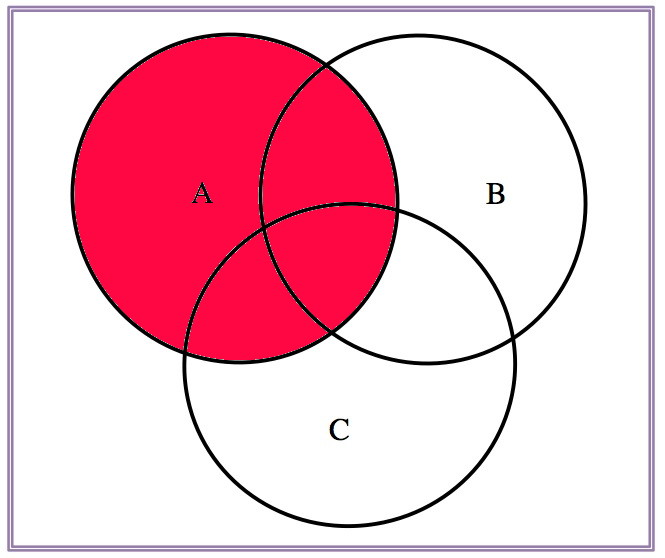
\includegraphics[width=\textwidth,height=2.08333in]{Images/proba1dibujos/distr11.jpg} & 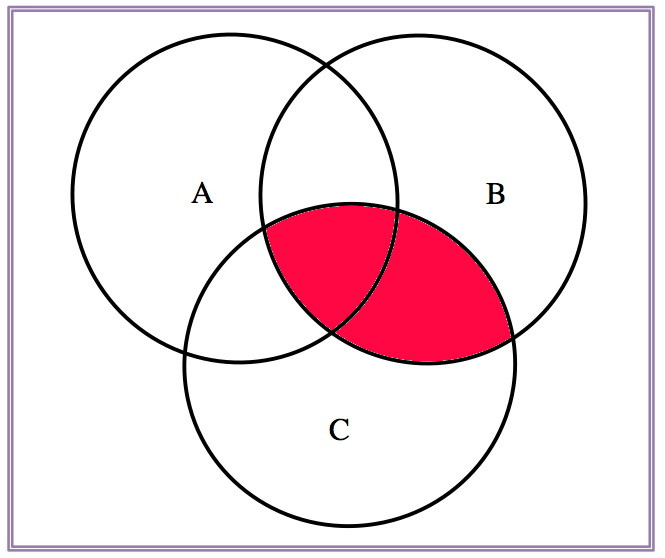
\includegraphics[width=\textwidth,height=2.08333in]{Images/proba1dibujos/distr12.jpg} & 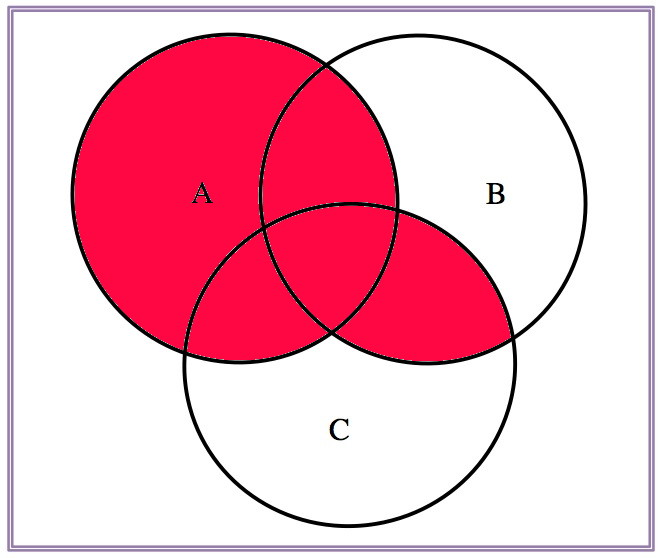
\includegraphics[width=\textwidth,height=2.08333in]{Images/proba1dibujos/distr13.jpg}\tabularnewline
\bottomrule
\end{longtable}

\hypertarget{propiedades-2}{%
\subsection{Propiedades}\label{propiedades-2}}

\begin{longtable}[]{@{}ccc@{}}
\toprule
\(A\cup B\) & \(A\cup C\) & \((A\cup B)\cap (A\cup C)\)\tabularnewline
\midrule
\endhead
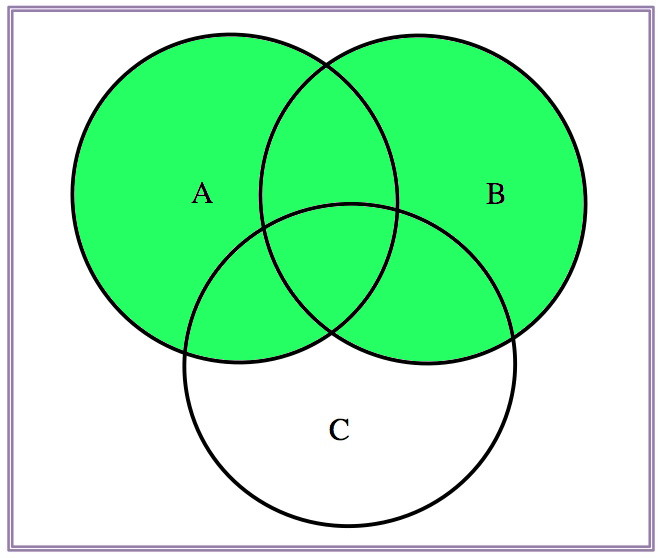
\includegraphics[width=\textwidth,height=2.08333in]{Images/proba1dibujos/distr21.jpg} & 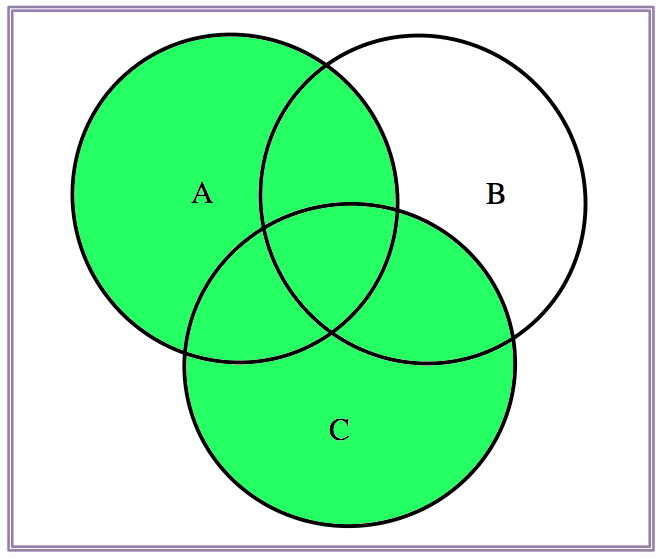
\includegraphics[width=\textwidth,height=2.08333in]{Images/proba1dibujos/distr22.jpg} & 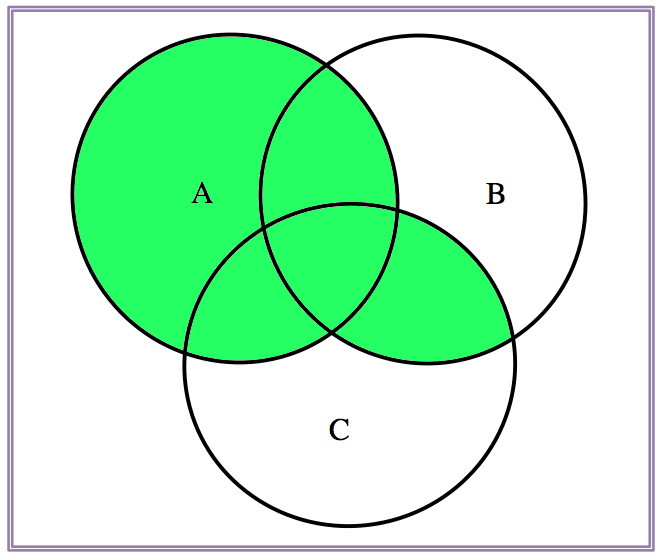
\includegraphics[width=\textwidth,height=2.08333in]{Images/proba1dibujos/distr23.jpg}\tabularnewline
\bottomrule
\end{longtable}

\hypertarget{propiedades-3}{%
\subsection{Propiedades}\label{propiedades-3}}

 Complementario del complementario
\[(A^c)^c=A\]

\begin{longtable}[]{@{}ccc@{}}
\toprule
\(A\) & \(A^c\) & \((A^c)^c\)\tabularnewline
\midrule
\endhead
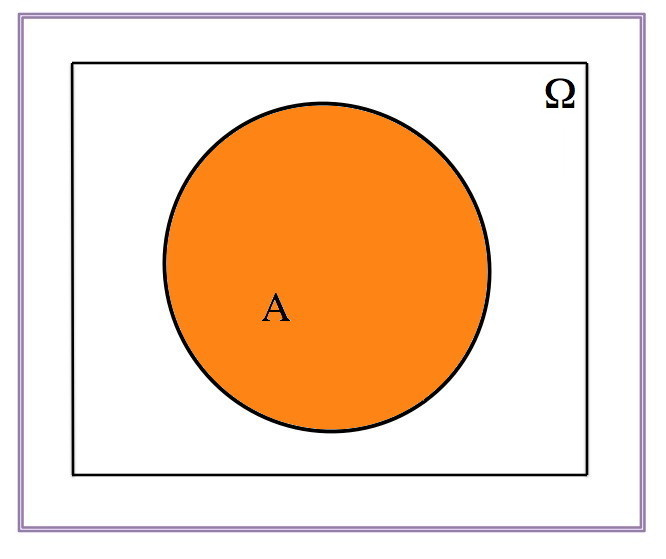
\includegraphics[width=\textwidth,height=2.08333in]{Images/proba1dibujos/dd2.jpg} & 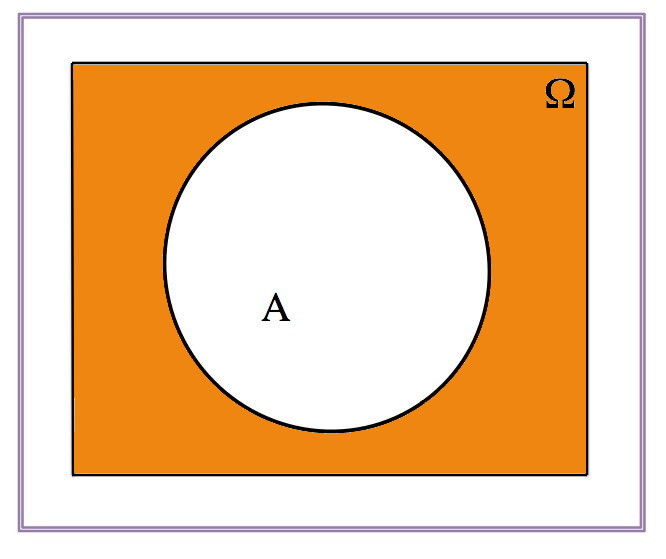
\includegraphics[width=\textwidth,height=2.08333in]{Images/proba1dibujos/dd1.jpg} & 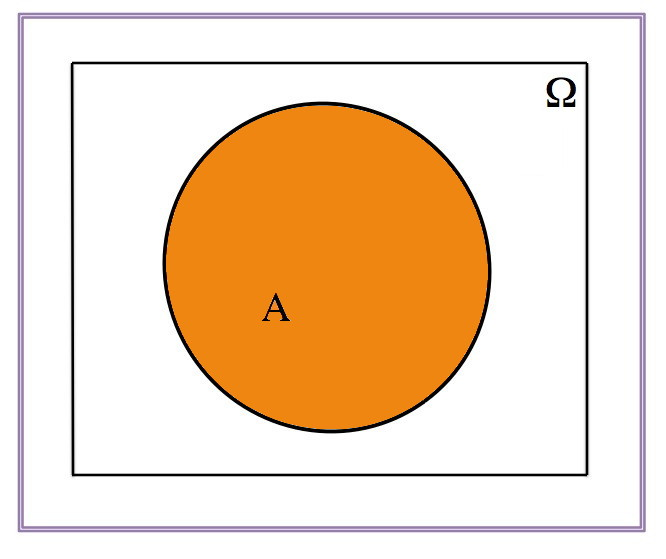
\includegraphics[width=\textwidth,height=2.08333in]{Images/proba1dibujos/dd3.jpg}\tabularnewline
\bottomrule
\end{longtable}

\hypertarget{propiedades-4}{%
\subsection{Propiedades}\label{propiedades-4}}

Leyes de De Morgan

\[(A\cup B)^c=A^c\cap B^c\]

\begin{longtable}[]{@{}cc@{}}
\toprule
\(A\cup B\) & \((A\cup B)^c\)\tabularnewline
\midrule
\endhead
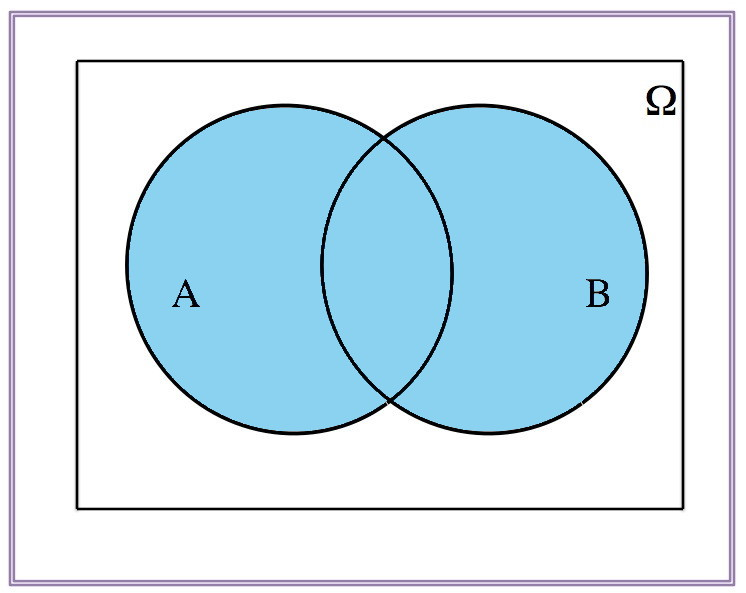
\includegraphics[width=\textwidth,height=2.08333in]{Images/proba1dibujos/demorgan6.jpg} & 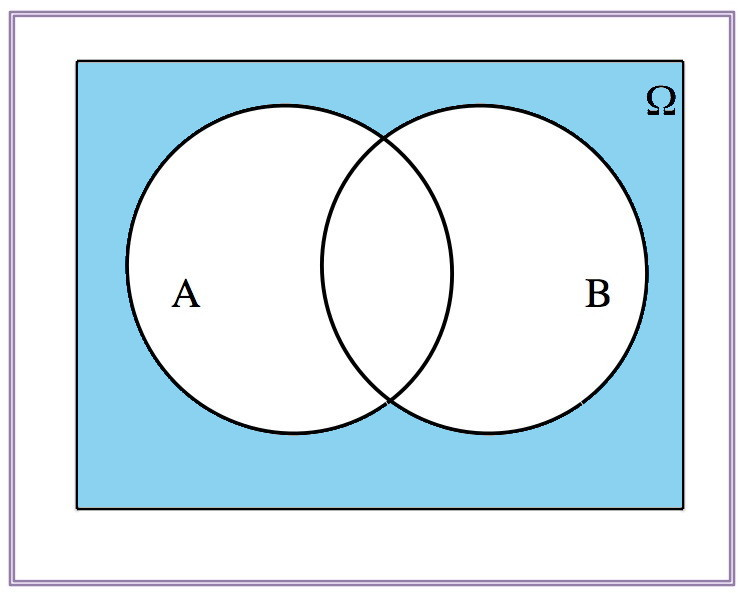
\includegraphics[width=\textwidth,height=2.08333in]{Images/proba1dibujos/demorgan7.jpg}\tabularnewline
\bottomrule
\end{longtable}

\hypertarget{propiedades-5}{%
\subsection{Propiedades}\label{propiedades-5}}

Leyes de De Morgan

\[(A\cup B)^c=A^c\cap B^c\]

\begin{longtable}[]{@{}ccc@{}}
\toprule
\(A^c\) & \(B^c\) & \(A^c\cap B^c\)\tabularnewline
\midrule
\endhead
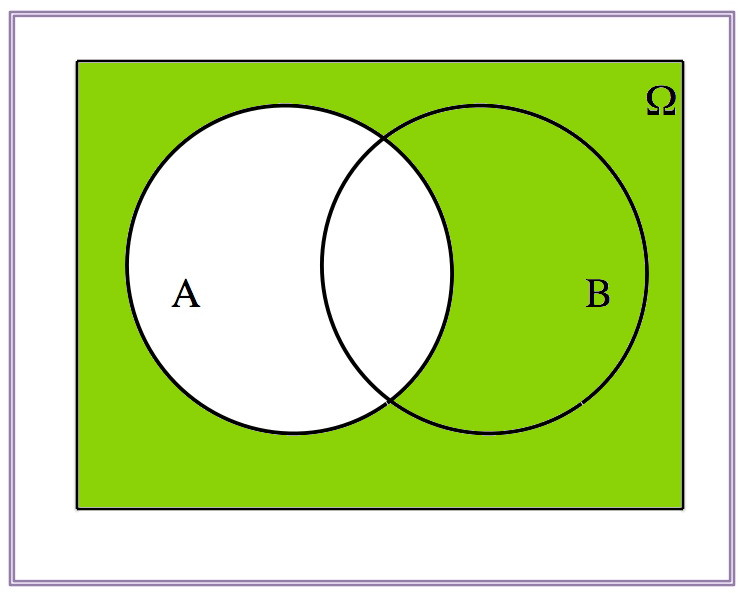
\includegraphics[width=\textwidth,height=2.08333in]{Images/proba1dibujos/demorgan8.jpg} & 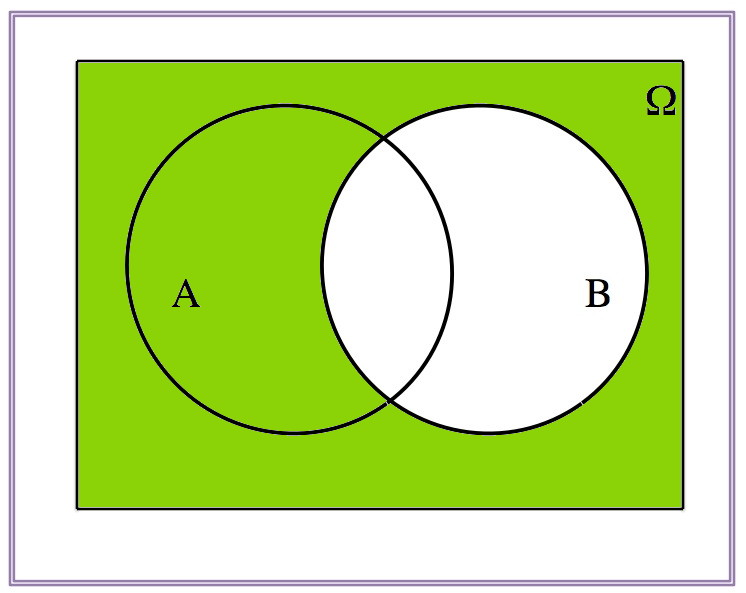
\includegraphics[width=\textwidth,height=2.08333in]{Images/proba1dibujos/demorgan9.jpg} & 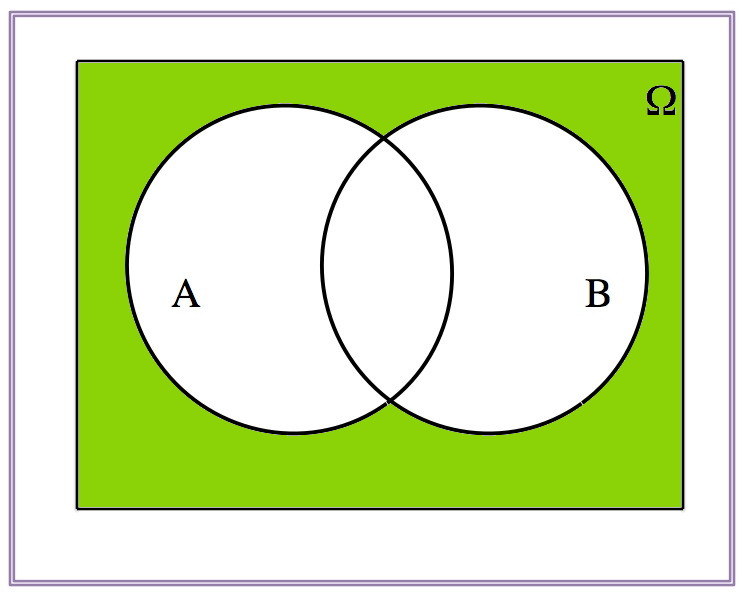
\includegraphics[width=\textwidth,height=2.08333in]{Images/proba1dibujos/demorgan10.jpg}\tabularnewline
\bottomrule
\end{longtable}

\hypertarget{propiedades-6}{%
\subsection{Propiedades}\label{propiedades-6}}

Leyes de De Morgan

\[(A\cap B)^c=A^c\cup B^c\]

\begin{longtable}[]{@{}cc@{}}
\toprule
\(A\cap B\) & \((A\cap B)^c\)\tabularnewline
\midrule
\endhead
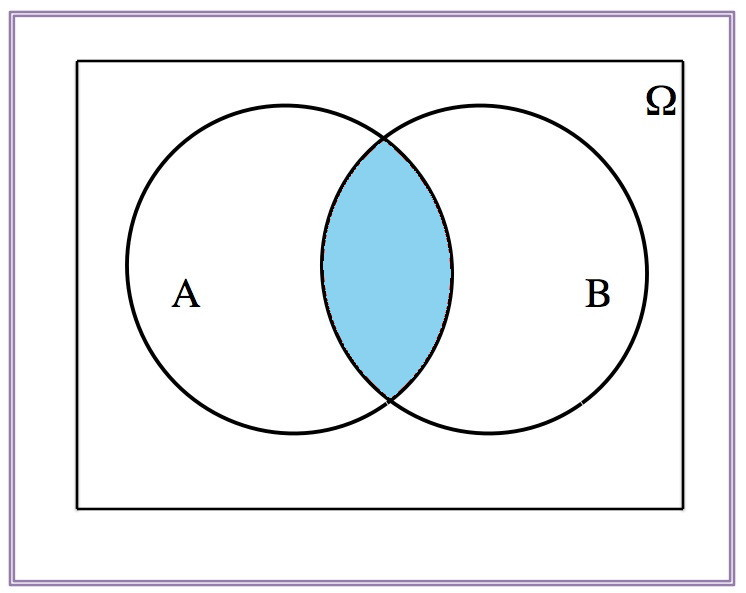
\includegraphics[width=\textwidth,height=2.08333in]{Images/proba1dibujos/demorgan1.jpg} & 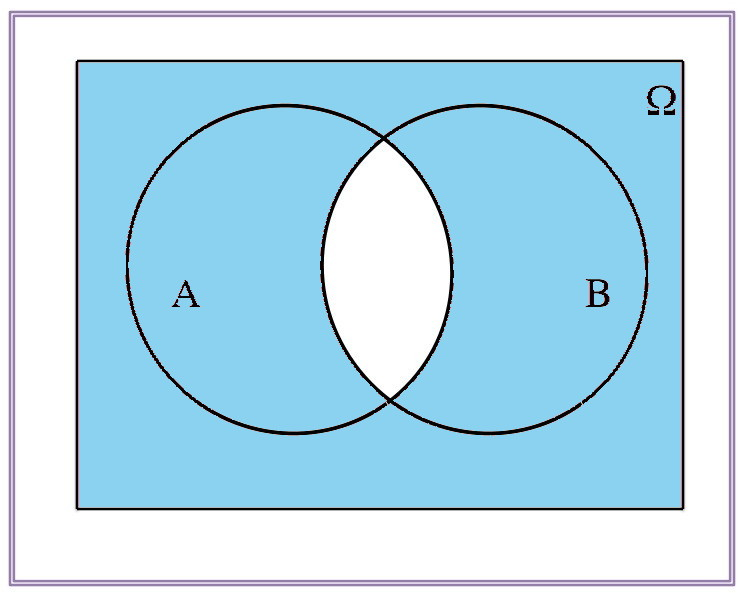
\includegraphics[width=\textwidth,height=2.08333in]{Images/proba1dibujos/demorgan2.jpg}\tabularnewline
\bottomrule
\end{longtable}

\hypertarget{propiedades-7}{%
\subsection{Propiedades}\label{propiedades-7}}

Leyes de De Morgan

\[(A\cap B)^c=A^c\cup B^c\]

\begin{longtable}[]{@{}ccc@{}}
\toprule
\(A^c\) & \(B^c\) & \(A^c\cup B^c\)\tabularnewline
\midrule
\endhead
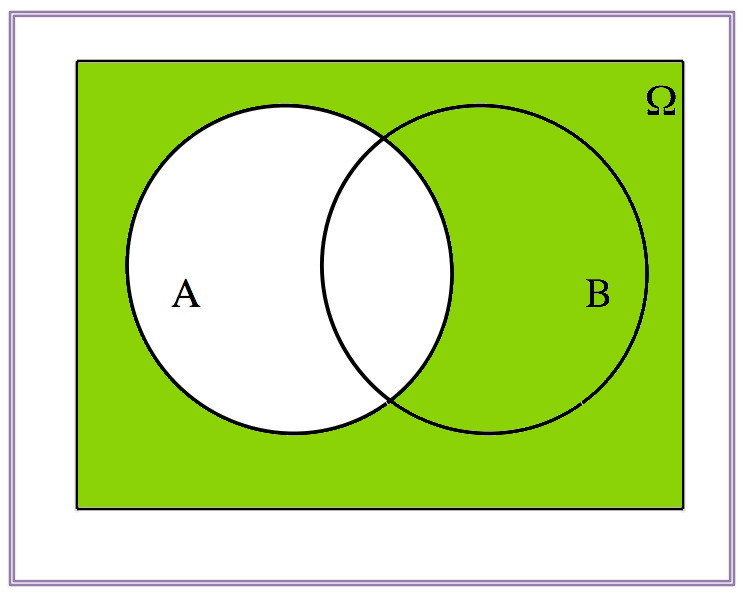
\includegraphics[width=\textwidth,height=2.08333in]{Images/proba1dibujos/demorgan3.jpg} & 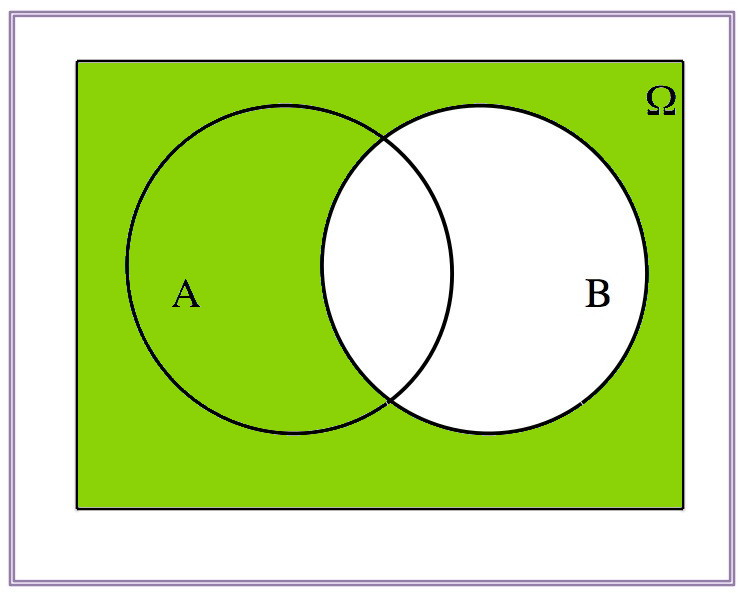
\includegraphics[width=\textwidth,height=2.08333in]{Images/proba1dibujos/demorgan5.jpg} & 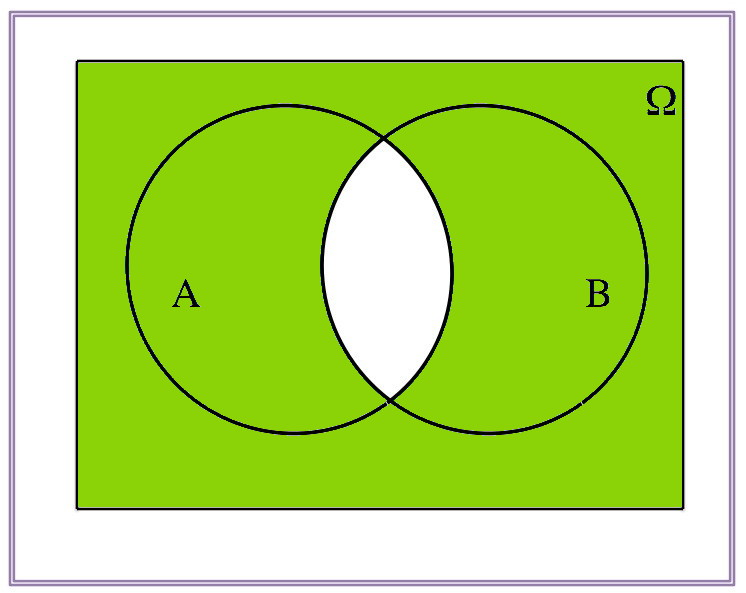
\includegraphics[width=\textwidth,height=2.08333in]{Images/proba1dibujos/demorgan4.jpg}\tabularnewline
\bottomrule
\end{longtable}

\hypertarget{definiciuxf3n-de-probabilidad}{%
\subsection{Definición de probabilidad}\label{definiciuxf3n-de-probabilidad}}

La probabilidad de un suceso es una puntuación (\emph{score}) numérico entre 0 y 1 que mide la verosimilitud de que este evento se produzca.

Esta verosimilitud puede estar justificada por

\begin{itemize}
\item
  Estimación personal
\item
  Estimación de expertos
\item
  La frecuencia con la que se da
\item
  Cálculo formal
\end{itemize}

\hypertarget{definiciuxf3n-de-probabilidad-1}{%
\subsection{Definición de probabilidad}\label{definiciuxf3n-de-probabilidad-1}}

Sea \(\Omega\) el espacio muestral de un experimento aleatorio.
Supongamos que el número de posibles resultados, por el momento, es finito.

Una probabilidad sobre \(\Omega\) es una aplicación \(P:\mathcal{P}(\Omega)\to [0,1]\) con las siguientes propiedades:

\begin{enumerate}
\def\labelenumi{\arabic{enumi}.}
\tightlist
\item
  \(0\leq P(A)\leq 1\), para todo suceso \(A\)
\item
  \(P(\Omega)=1\)
\item
  Si \(\{A_1,A_2,\ldots,A_n\}\) son sucesos disjuntos dos a dos, entonces
\end{enumerate}

\[
P(A_1\cup A_2\cup \cdots \cup A_n)=P(A_1)+P(A_2)+\cdots +P(A_n)
\]

Si \(a\in \Omega\) es un suceso elemental cometeremos el abuso de notación de poner \(P(a)\) en lugar de \(P(\{a\})\)

\hypertarget{ejemplo-grupos-sanguxedneos}{%
\subsection{Ejemplo: grupos sangíneos}\label{ejemplo-grupos-sanguxedneos}}

\textbf{Ejemplo}

En la página de la \href{http://www.donasang.org/que-es-la-sang/es_frequencies-dels-diferents-grups.html}{Fundación Banco de Sangre y Tejidos de las Islas Baleares} podemos encontrar información sobre los porcentajes de tipos de sangre de los donantes de las Islas Baleares:

\[A: 46\%; B: 7.5\%; AB: 3.5\%; O: 43\%\]

¿Cuál es la probabilidad de que un balear donante de sangre no sea del tipo 0?

\textbf{Experimento aleatorio:} tipo de sangre de un paciente humano

\[\Omega=\{\mbox{A,B,AB,O}\}\]

\textbf{Probabilidad} de un suceso: se asimila al porcentaje observado de individuos

\textbf{Suceso:} \(\{\mbox{O}\}^c=\{\mbox{A,B,AB}\}\)

\[P(\{\mbox{O}\}^c)\!=\!P(\{\mbox{A,B,AB}\})\!=\!
P(\mbox{A})+P (\mbox{B})+P(\mbox{AB})\!=\!0.57\]

\hypertarget{propiedades-8}{%
\subsection{Propiedades}\label{propiedades-8}}

Propiedades básicas de la probabilidad

\begin{itemize}
\item
  \(P(\emptyset)=0\)
\item
  \(P(A-B)=P(A)-P(A\cap B)\) porque \(P(A)=P(A-B)+P(A\cap B)\)
\end{itemize}

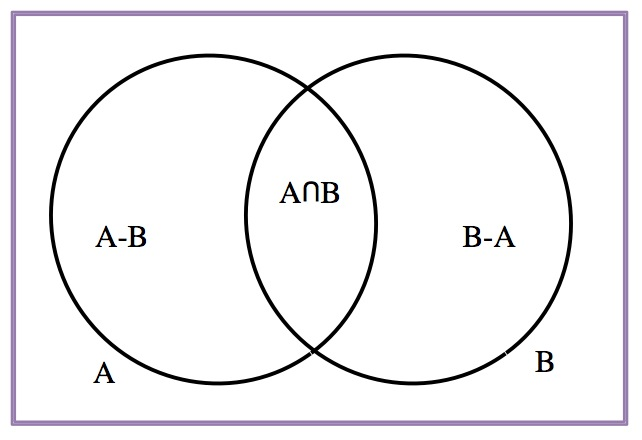
\includegraphics[width=\textwidth,height=2.08333in]{Images/proba1dibujos/A-B.jpg}

\begin{itemize}
\item
  Si \(B\subseteq A\), entonces \(0\leq P(B)\leq P(A)\)
\item
  \(P(A^c)=1-P(A)\)
\end{itemize}

\hypertarget{propiedades-9}{%
\subsection{Propiedades}\label{propiedades-9}}

\begin{itemize}
\tightlist
\item
  \(P(A\cup B)=P(A)+P(B)-P(A\cap B)\) porque
\end{itemize}

\begin{eqnarray*}
P(A)+P(B)-P(A\cap B) &=& P(A-B)+P(A\cap B)+\\
 & & P(B-A)+ P(A\cap  B)-P(A\cap  B)\\
&=& P(A-B)+P(A\cap B)+ P(B-A) \\
&=& P(A\cup B)
\end{eqnarray*}

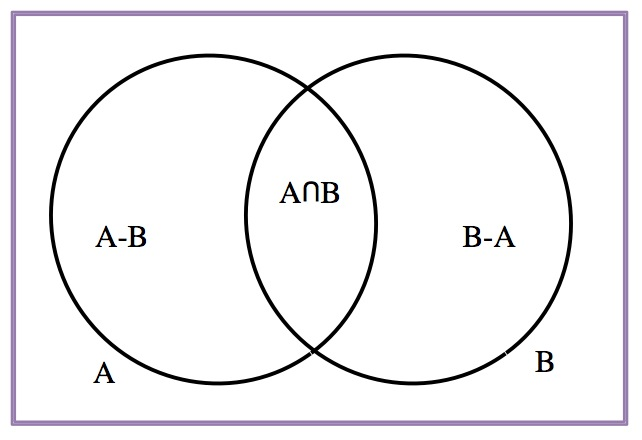
\includegraphics[width=\textwidth,height=2.08333in]{Images/proba1dibujos/A-B.jpg}

\hypertarget{propiedades-10}{%
\subsection{Propiedades}\label{propiedades-10}}

\begin{itemize}
\tightlist
\item
  \begin{eqnarray*}
  P(A\cup B\cup C)&=&P(A)+P(B)+P(C)  \\ &&-P(A\cap B)-P(A\cap C)-P(B\cap C)  +P(A\cap B\cap C)
  \end{eqnarray*}
\end{itemize}

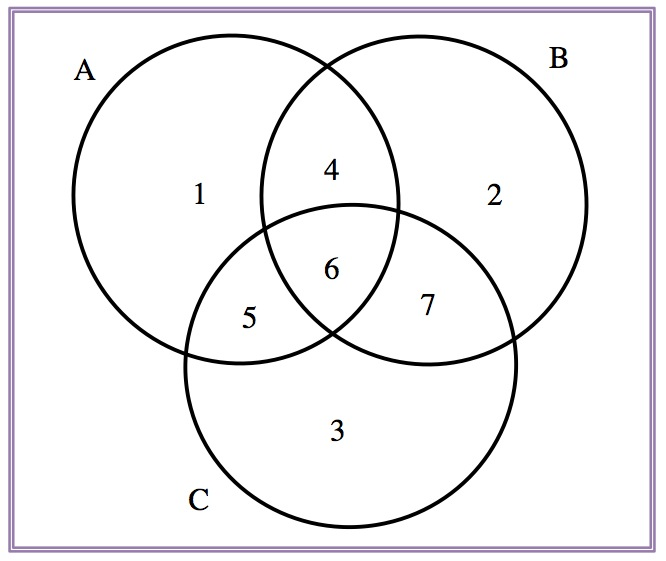
\includegraphics[width=\textwidth,height=2.08333in]{Images/proba1dibujos/tresconjunts.jpg}

\[P(A\cup B\cup C)=P(1)+P(2)+P(3)+P(4)+P(5)+P(6)+P(7)\]

\hypertarget{propiedades-11}{%
\subsection{Propiedades}\label{propiedades-11}}

\begin{itemize}
\item
  Si \(A=\{a_1,a_2,\ldots,a_k\}\), entonces
  \[
  P(A)=P(a_1)+P(a_2)+\cdots+P(a_k)
  \]
\item
  Si todos los sucesos elementales tienen la misma probabilidad,
  \[
  P(A)=\frac{|A|}{|\Omega|}\Big(=\frac{\mbox{casos favorables}}{\mbox{casos posibles}}\Big)
  \]
\end{itemize}

\hypertarget{ejemplo-frecuencia-de-vocales}{%
\subsection{Ejemplo: Frecuencia de vocales}\label{ejemplo-frecuencia-de-vocales}}

\textbf{Ejemplo}

Los porcentajes de vocales de un determinado idioma (de alfabeto latino) según la \href{https://es.wikipedia.org/wiki/Frecuencia_de_aparici\%C3\%B3n_de_letras}{Wikipedia} son:

\[A: 18.7\%; E: 26.1\%; I: 25.7\%; O: 24.4\% U: 5.1\%\]

¿Cuál es la probabilidad que una vocal escogida al azar de este idioma sea una E o una O?

El espacio muestral del experimento es \(\Omega=\{A,E,I,O,U\}\).

El suceso que deseamos analizar es \(\{E,0\}\).

Y su probabilidad es

\[P(\{E,O\})=P(E)+P(O)=0.261+0.244=0.505.\]

\hypertarget{ejemplo-consumo-de-drogas}{%
\subsection{Ejemplo: Consumo de drogas}\label{ejemplo-consumo-de-drogas}}

Segun un árticulo de \href{https://elpais.com/politica/2019/01/02/actualidad/1546426491_623324.html}{El País}, en un control especial de la policía el \(0.1\%\) de todos los conductores analizados en un control de tráfico dan positivo en un el test en cocaína, y el \(1\%\) da positivo en cannabis. Un \(1.05\%\) da positivo en alguno de los dos test.

¿Cuál es la probabilidad que un individuo analizado en el control de drogas escogido al azar no de positivo en ninguno de lo dos test?

Los sucesos elementales del enunciado del problema son:

\begin{itemize}
\tightlist
\item
  \(A\): dar positivo en cocaína; \(P(A)=0.001\)
\item
  \(B\): dar positivo en cannabis; \(P(B)=0.01\)
\end{itemize}

En este caso nos interesa estudiar los sucesos:

\begin{itemize}
\tightlist
\item
  \(A\cup B\): dar positivo en alguno de los dos test; \(P(A\cup B)=0.0105\)
\item
  \((A\cup B)^c\): no dar positivo en ninguno de los test
\end{itemize}

de donde, por tanto:
\[P((A\cup B)^c)=1-P(A\cup B)=1-0.0105=0.9895.\]

\hypertarget{ejemplos-consumo-de-drogas}{%
\subsection{Ejemplos: Consumo de drogas}\label{ejemplos-consumo-de-drogas}}

\textbf{Ejemplo}

En un control especial de la policía el \(0.1\%\) de todos los conductores analizados en un control de tráfico dan positivo en un el test en cocaína, y el \(1\%\) da positivo en cannabis. Un \(1.05\%\) da positivo en alguno de los dos test.

¿Cuál es la probabilidad que un analizado al azar de positivo en los dos test en cocaína y cannabis?

Los sucesos elementales son:

\begin{itemize}
\tightlist
\item
  \(A\): dar positivo en cocaína; \(P(A)=0.001\)
\item
  \(B\): dar positivo en cannabis; \(P(B)=0.01\)
\end{itemize}

En este caso nos interesa estudiar los sucesos:

\begin{itemize}
\tightlist
\item
  \(A\cup B\): dar positivo en algún de los dos test; \(P(A\cup B)=0.0105\)
\item
  \(A\cap B\): dar positivo en los dos test
\end{itemize}

de donde, por tanto:

\[\begin{array}{rl}
{P(A\cap B)} &{=P(A)+P(B)-P(A\cup B)}\\ &{=0.001+0.01-0.0105=0.0005}
\end{array}\]

\hypertarget{ejemplo-control-de-drogas}{%
\subsection{Ejemplo: Control de drogas}\label{ejemplo-control-de-drogas}}

\textbf{Ejemplo}

En un control especial de la policía el \(0.1\%\) de todos los conductores analizados en un control de tráfico dan positivo en un el test en cocaína, y el \(1\%\) da positivo en cannabis. Un \(1.05\%\) da positivo en alguno de los dos test.

¿Cuál es la probabilidad de que un conductor analizado de positivo en cocaína pero no en cannabis?

Los sucesos elementales son:

\begin{itemize}
\tightlist
\item
  \(A\): dar positivo en cocaína; \(P(A)=0.001\)
\item
  \(B\): dar positivo en cannabis; \(P(B)=0.01\)
\end{itemize}

En este caso nos interesa estudiar los sucesos:

\begin{itemize}
\tightlist
\item
  \(A\cap B\): dar positivo en los dos test; \(P(A\cap B)=0.0005\)
\item
  \(B-A\): dar positivo en cocaína pero no en cannabis
\end{itemize}

de donde, por tanto:

\[P(B-A) =P(B)-P(A\cap B) =0.01-0.0005=0.0095\]

\hypertarget{probabilidad-condicionada}{%
\section{Probabilidad condicionada}\label{probabilidad-condicionada}}

\hypertarget{probabilidad-condicionada-1}{%
\subsection{Probabilidad condicionada}\label{probabilidad-condicionada-1}}

 Probabilidad condicionada: Dados dos sucesos \(A\) y \(B\), con \(P(A)>0\), la probabilidad \(P(B|A)\) de \(B\) condicionado a \(A\) es la probabilidad

\begin{itemize}
\tightlist
\item
  de que suceda \(B\) suponiendo que pasa \(A\)
\item
  de que si pasa \(A\), entonces suceda \(B\)
\item
  de que un resultado de \(A\) también pertenezca a \(B\)
\end{itemize}

Se calcula a través de la definición:

\[
P(B|A)=\frac{P(A\cap B)}{P(A)}
\]

\hypertarget{ejemplo-frecuencia-guxe9nero-y-gafas}{%
\subsection{Ejemplo: frecuencia género y gafas}\label{ejemplo-frecuencia-guxe9nero-y-gafas}}

\textbf{Ejemplo}

En una clase de 20 hombres y 30 mujeres, 15 hombres y 18 mujeres llevan gafas. Contestemos las siguientes preguntas:

\begin{itemize}
\tightlist
\item
  ¿Cuál es la probabilidad de que un alumno lleve gafas?
\end{itemize}

\[
\frac{33}{50}
\]

\begin{itemize}
\tightlist
\item
  ¿Cuál es la probabilidad de que un alumno sea mujer y lleve gafas?
\end{itemize}

\[
\frac{18}{50}
\]

\hypertarget{ejemplo-sexo-y-gafas}{%
\subsection{Ejemplo: sexo y gafas}\label{ejemplo-sexo-y-gafas}}

\textbf{Ejemplo}

En una clase de 20 hombres y 30 mujeres, 15 hombres y 18 mujeres llevan gafas. Contestemos las siguientes preguntas:

\begin{itemize}
\tightlist
\item
  ¿Cuál es la probabilidad de que un chica lleve gafas?
\end{itemize}

\[
\frac{18}{30}=\frac{18/50}{30/50}=\frac{P(\mbox{mujer  y gafas})}{P(\mbox{mujer})}
\]

\begin{itemize}
\tightlist
\item
  Si escogemos un estudiante al azar ¿Cuál es la probabilidad que si es mujer, entonces lleve gafas?
\end{itemize}

\[
\frac{18}{30}
\]

\hypertarget{ejemplo}{%
\subsection{Ejemplo}\label{ejemplo}}

\textbf{Ejemplo}

En una clase de 20 hombres y 30 mujeres, 15 hombres y 18 mujeres llevan gafas. Contestemos las siguientes preguntas:

\begin{itemize}
\tightlist
\item
  ¿Cuál es la probabilidad de que un alumno que lleve gafas sea mujer?
\end{itemize}

\[
\frac{18}{33}=\frac{18/50}{33/50}=\frac{P(\mbox{mujer y gafas})}{P(\mbox{gafas})}
\]

\begin{itemize}
\tightlist
\item
  Si escogemos un estudiante al azar ¿Cuál es la probabilidad de que si lleva gafas, entonces sea mujer?
  \[
  \frac{18}{33}
  \]
\end{itemize}

\hypertarget{atenciuxf3n}{%
\subsection{¡Atención!}\label{atenciuxf3n}}

Hay que distinguir bien entre

\begin{itemize}
\tightlist
\item
  \(P(A\cap B)\): probabilidad de \(A\) \(\color{red}{\text{y}}\) \(B\)
\end{itemize}

\emph{Probabilidad de que sea mujer y lleve gafas}

\begin{itemize}
\tightlist
\item
  \(P(A|B)\): probabilidad de que \(\color{red}{\text{si}}\) pasa \(B\), \(\color{red}{\text{entonces}}\) pase \(A\).
\end{itemize}

\emph{Probabilidad de que, si es mujer, lleve gafas}

Cuando utilizamos probabilidad condicional \(P(A|B)\) estamos restringiendo el espacio muestral a \(B\)

\hypertarget{probabilidad-condicionada.-propiedades}{%
\subsection{Probabilidad condicionada. Propiedades}\label{probabilidad-condicionada.-propiedades}}

La probabilidad condicionada es una probabilidad

Proposición

Sea \(A\subseteq \Omega\) un suceso tal que \(P(A)>0\). entonces

\[
\begin{array}{rccl}
P(-|A):& \mathcal{P}(\Omega) & \to & [0,1]\\
&B & \mapsto & P(B|A)
\end{array}
\]
satisface las propiedades de las probabilidades, como por ejemplo:

\[
\begin{array}{l}
P(B^c|A)=1-P(B|A)\\
P(B_1\cup B_2|A)=P(B_1|A)+P(B_2|A)-P(B_1\cap B_2|A)
\end{array}
\]

\textbf{Ejercicio}

Escribid el resto de propiedades que cumpliría una probabilidad condicionada al evento \(A\).

\hypertarget{ejemplos}{%
\subsection{Ejemplos}\label{ejemplos}}

\textbf{Ejemplo}

Un 15\% de los adultos son hipertensos, un 25\% de los adultos creen que son hipertensos, y un 9\% de los adultos son hipertensos y creen que lo son.

Si un adulto cree que es hipertenso, ¿cuál es la probabilidad que lo sea?

Sean los sucesos

\begin{itemize}
\tightlist
\item
  \(A\): ser hipertenso; \(P(A)=0.15\)
\item
  \(B\): creer ser hipertenso; \(P(B)=0.25\)
\end{itemize}

entonces podemos definir el suceso:

\begin{itemize}
\tightlist
\item
  \(A\cap B\): ser hipertenso y creerlo; \(P(A\cap B)=0.09\)
\end{itemize}

de donde, la probabilidad condicionada de ser hipertenso creyéndonos que lo somos es:

\[P(A|B)=\dfrac{P(A\cap B)}{P(B)}=\dfrac{0.09}{0.25}=0.36\]

\hypertarget{ejemplo-1}{%
\subsection{Ejemplo}\label{ejemplo-1}}

\textbf{Ejemplo}

Un 15\% de los adultos son hipertensos, un 25\% de los adultos creen que son hipertensos, y un 9\% de los adultos son hipertensos y creen que lo son.

Si un adulto es hipertenso, ¿cuál es la probabilidad que crea que lo es?

Si tenemos los sucesos:

\begin{itemize}
\tightlist
\item
  \(A\): ser hipertenso;
\item
  \(B\): creer ser hipertenso
\end{itemize}

entonces buscamos la probabilidad \(P(B|A)\):

\[
\begin{array}{rl}
P(B|A) & =\dfrac{P(A\cap B)}{P(A)}=\dfrac{0.09}{0.15}=
0.6
\end{array}
\]

\hypertarget{ejemplos-duxedgitos-de-control}{%
\subsection{Ejemplos: dígitos de control}\label{ejemplos-duxedgitos-de-control}}

\textbf{Ejemplo}

Un dígito de control de error toma el valor 0 en el 99\% de los casos en que hay un error. Si la probabilidad de error en un mensaje es del \(0.5\%\). \textbackslash{}blue\{¿cuál es la probabilidad de que el mensaje sea erróneo y el código de error tenga valor 0?

\begin{itemize}
\tightlist
\item
  \(B\): mensaje con error; \(P(B)=0.005\)
\item
  \(A\): código de error vale 0;
\item
  \(P(A|B)=0.99\)
\end{itemize}

entonces:
\[P(A\cap B)=P(B)\cdot P(A|B)=0.005\cdot 0.99=0.00495\]

\hypertarget{ejemplos-1}{%
\subsection{Ejemplos}\label{ejemplos-1}}

\textbf{Ejemplo}

Un 50\% de correos recibidos en un servidor llevan adjuntos y un 65\% son publicidad no deseada (SPAM). Sólo un 15\% de estos correos no llevan adjuntos y no son SPAM.

\begin{itemize}
\tightlist
\item
  ¿Cuál es la probabilidad que un correo lleve adjunto si es SPAM?
\item
  ¿Cuál es la probabilidad que un correo \textbf{no} tenga adjuntos si \textbf{no} es SPAM?
\end{itemize}

\hypertarget{ejemplos-2}{%
\subsection{Ejemplos}\label{ejemplos-2}}

\textbf{Ejemplo}

Un 50\% de correos recibidos en un servidor llevan adjuntos y un 65\% son publicidad no deseada (SPAM). Sólo un 15\% de estos correos no llevan adjuntos y no son SPAM.

\begin{itemize}
\tightlist
\item
  ¿Cuál es la probabilidad que un correo lleve adjunto si es SPAM?
\end{itemize}

\begin{itemize}
\tightlist
\item
  \(A\): llevar adjuntos; \(P(A)=0.5\)
\item
  \(S\): SPAM; \(P(S)=0.65\)
\item
  \(A^c\cap S^c=(A\cup S)^c\): no llevar adjunto y no ser SPAM; \(P((A\cup S)^c)=0.15\)
\end{itemize}

\[P(A|S)=\dfrac{P(A\cap S)}{P(S)}=?\]

\hypertarget{ejemplos-3}{%
\subsection{Ejemplos}\label{ejemplos-3}}

\textbf{Ejemplo}

Un 50\% de correos recibidos en un servidor llevan adjuntos y un 65\% son publicidad no deseada (SPAM). Sólo un 15\% de estos correos no llevan adjuntos y no son SPAM.

\begin{itemize}
\tightlist
\item
  ¿Cuál es la probabilidad que un correo lleve adjunto si es SPAM?
\end{itemize}

\begin{itemize}
\item
  \(P(A)=0.5, P(S)=0.65, P(A^c\cap S^c)=P((A\cup S)^c)=0.15\)
\item
  \(P(A\cup S)=1-P((A\cup S)^c)=0.85\)
\item
  \(P(A\cap S)=P(A)+P(S)-P(A\cup S)=0.3\)
\end{itemize}

\[P(A|S)=\dfrac{P(A\cap S)}{P(S)}=\dfrac{0.3}{0.65}\approx 0.46\]

\hypertarget{ejemplos-spam-continuaciuxf3n}{%
\subsection{Ejemplos SPAM continuación}\label{ejemplos-spam-continuaciuxf3n}}

\textbf{Ejemplo}

Un 50\% de correos recibidos en un servidor llevan adjuntos y un 65\% son publicidad no deseada (SPAM). Sólo un 15\% de estos correos no llevan adjuntos y no son SPAM.

\begin{itemize}
\tightlist
\item
  ¿Cuál es la probabilidad de que un correo no lleve adjuntos si no es SPAM?
\end{itemize}

\begin{itemize}
\tightlist
\item
  \(P(A)=0.5, P(S)=0.65, P(A^c\cap S^c)=P((A\cup S)^c)=0.15\)
\end{itemize}

\[P(A^c|S^c)=\dfrac{P(A^c\cap S^c)}{P(S^c)}=\dfrac{P(A^c\cap S^c)}{1-P(S)}=\dfrac{0.15}{0.35}\approx 0.43\]

\hypertarget{teorema-de-la-probabilidad-total}{%
\subsection{Teorema de la probabilidad total}\label{teorema-de-la-probabilidad-total}}

Teorema de la probabilidad total

Dados dos sucesos \(A\) y \(B\) se tiene que

\[
\begin{array}{rl}
P(B)&= P(B\cap A) +P(B\cap A^c)\\
& =P(A)\cdot P(B|A)+ P(A^c)\cdot P(B|A^c)
\end{array}
\]

\hypertarget{teorema-de-la-probabilidad-total-1}{%
\subsection{Teorema de la probabilidad total}\label{teorema-de-la-probabilidad-total-1}}

Partición del espacio espacio muestral

Los sucesos \(A_1,A_2,\ldots, A_n\) son una \textbf{partición} del espacio muestral \(\Omega\) de un determinado experimento aleatorio, si cumplen las condiciones siguientes:

\begin{enumerate}
\def\labelenumi{\arabic{enumi}.}
\tightlist
\item
  \(A_1\cup A_2\cup\ldots\cup A_n=\Omega\)
\item
  \(A_1,A_2,\ldots,A_n\) son incompatibles dos a dos (\(A_i\cap A_j=\emptyset\))
\end{enumerate}

Teorema de la probabilidad total

Sea \(A_1,A_2,\ldots,A_n\) una partición de \(\Omega\). Sea \(B\) un suceso cualquiera. Entonces

\[
\begin{array}{rl}
P(B)&= P(B\cap A_1)+\cdots +P(B\cap A_n)\\
& =P(A_1)\cdot P(B|A_1)+\ldots+P(A_n)\cdot P(B|A_n)
\end{array}
\]

\hypertarget{ejemplos-4}{%
\subsection{Ejemplos}\label{ejemplos-4}}

\textbf{Ejemplo}

Un dígito de control de error toma el valor 0 en un \(99\%\) de los casos en que hay un error y en un \(5\%\) de los mensajes sin error.
La probabilidad de error en un mensaje es del \(0.5\%\)

¿Cuál es la probabilidad de que un mensaje escogido al azar tenga el dígito de control a 0?

Sean los sucesos del enunciado:

\begin{itemize}
\tightlist
\item
  \(B\): mensaje con error; \(P(B)=0.005\)
\item
  \(A\): código de error vale 0;
\end{itemize}

entonces obtenemos las probabilidades a partir del enunciado:

\begin{itemize}
\tightlist
\item
  \(P(A|B)=0.99\)
\item
  \(P(A|B^c)= 0.05\)
\end{itemize}

y por tanto,

\[
\begin{array}{rl}
P(A) & =P(B)\cdot P(A|B)+P(B^c)\cdot P(A|B^c)\\ &
=0.005\cdot 0.99+0.995\cdot 0.05=0.0547\end{array}
\]

\hypertarget{clasificaciuxf3n-o-diagnuxf3sticos}{%
\subsection{Clasificación o Diagnósticos}\label{clasificaciuxf3n-o-diagnuxf3sticos}}

Consideremos alguna de las siguientes situaciones:

\begin{itemize}
\tightlist
\item
  Un algoritmo detecta si una transacción con tarjeta de crédito es fraude o no.
\item
  Un algoritmo detecta si tiene o no que mostrar un anuncio en una web.
\item
  Un prueba de embarazo.
\item
  Una prueba médica para una enfermedad concreta.
\end{itemize}

Nos ceñiremos a la casuística más elemental el algoritmo de clasificación o la diagnosis solo da dos resultado \textbf{Positivo} (sí tienes la enfermedad, sí es un fraude) o \textbf{Negativo} (en caso contrario).

\hypertarget{clasificaciuxf3n-o-diagnuxf3sticos-1}{%
\subsection{Clasificación o Diagnósticos}\label{clasificaciuxf3n-o-diagnuxf3sticos-1}}

En todas estas situaciones podemos calcular lo que se llama \textbf{matriz de confusión} que representa todas las situaciones posibles. En el caso de estudiar una condición de tipo binario,

\begin{longtable}[]{@{}ccc@{}}
\toprule
& El Test da Positivo & El Test da Negativo\tabularnewline
\midrule
\endhead
Condición Positiva & Correcto & Error\tabularnewline
Condición Negativa & Error & Correcto\tabularnewline
\bottomrule
\end{longtable}

\hypertarget{clasificaciuxf3n-o-diagnuxf3sticos-2}{%
\subsection{Clasificación o Diagnósticos}\label{clasificaciuxf3n-o-diagnuxf3sticos-2}}

En general los modelos y algoritmos de clasificación suelen aportar puntuaciones (\emph{scores}) que determinan el grado de pertenencia a una clase, o que miden si dos objetos están en la misma clase.

Así el resultado del clasificador o del diagnóstico puede ser:

\begin{itemize}
\tightlist
\item
  \textbf{un número real}, en cuyo caso debe clasificador entre cada clase debe determinarse por un valor umbral (\emph{threshold}) por ejemplo para determinar si una persona está estresado podemos dar un \emph{scores} entre 0 y 1 (1 máximo estrés 0 estrés nulo):
\item
  \textbf{un resultado discreto} que indica directamente una de las clases (esto es necesario si es un algoritmo que debe decidir qué hacer con el objeto.
\end{itemize}

\hypertarget{clasificaciuxf3n-o-diagnuxf3sticos-3}{%
\subsection{Clasificación o Diagnósticos}\label{clasificaciuxf3n-o-diagnuxf3sticos-3}}

\hypertarget{clasificaciuxf3n-o-diagnuxf3sticos-4}{%
\subsection{Clasificación o Diagnósticos}\label{clasificaciuxf3n-o-diagnuxf3sticos-4}}

Positivos y Negativos en Clasificación

Consideremos un problema de predicción de clases binario, en la que los resultados se etiquetan positivos (P) o negativos (N). Hay cuatro posibles resultados a partir de un clasificador binario como el propuesto.

\begin{itemize}
\tightlist
\item
  Si el resultado de una exploración es P y el valor dado es también P, entonces se conoce como un Verdadero Positivo (VP).
\item
  Sin embargo si el valor real es N entonces se conoce como un Falso Positivo (FP).
\item
  De igual modo, tenemos un Verdadero Negativo (VN) cuando tanto la exploración como el valor dado son N.
\item
  Un Falso Negativo (FN) cuando el resultado de la predicción es N pero el valor real es P.
\end{itemize}

\hypertarget{clasificaciuxf3n-o-diagnuxf3sticos-5}{%
\subsection{Clasificación o Diagnósticos}\label{clasificaciuxf3n-o-diagnuxf3sticos-5}}

Un ejemplo aproximado de un problema real es el siguiente: consideremos una prueba diagnóstica que persiga determinar si una persona tiene una cierta enfermedad.

\begin{itemize}
\tightlist
\item
  Un falso positivo en este caso ocurre cuando la prueba predice que el resultado es positivo, cuando la persona no tiene realmente la enfermedad.
\item
  Un falso negativo, por el contrario, ocurre cuando el resultado de la prueba es negativo, sugiriendo que no tiene la enfermedad cuando realmente sí la tiene.
\end{itemize}

\hypertarget{clasificaciuxf3n-o-diagnuxf3sticos-6}{%
\subsection{Clasificación o Diagnósticos}\label{clasificaciuxf3n-o-diagnuxf3sticos-6}}

En un diagnósticos de una cierta condición (por ejemplo, test embarazo, test de enfermedad), tenemos dos tipos de sucesos:

\begin{itemize}
\tightlist
\item
  \(T\): el test da positivo
\item
  \(M\): el sujeto satisface la condición
\end{itemize}

 Falsos Positivos y Falsos Negativos

\begin{itemize}
\tightlist
\item
  \textbf{Falsos positivos} \(T\cap M^c\): El test da positivo, pero la condición no es da
\item
  \textbf{Coeficiente de falsos positivos} \(P(T|M^c)\)
\item
  \textbf{Falsos negativos} \(T^c\cap M\): El test da negativo, pero la condición sí que se da
\item
  \textbf{Coeficiente de falsos negativos}: \(P(T^c|M)\)
\end{itemize}

\hypertarget{clasificaciuxf3n-o-diagnuxf3sticos-7}{%
\subsection{Clasificación o Diagnósticos}\label{clasificaciuxf3n-o-diagnuxf3sticos-7}}

\textbf{Ejemplo}

Un test diseñado para diagnosticar una determinada enfermedad tiene un coeficiente de falsos negativos de 0.06, y un coeficiente de falsos positivos de 0.04. En un estudio masivo se observa que un 15\% de la población da positivo al test.

¿Cuál es la probabilidad que una persona escogida aleatoriamente tenga esta enfermedad?

Los datos del problema son:

\begin{itemize}
\tightlist
\item
  \(T\): dar positivo al test; \(P(T)=0.15\)
\item
  \(M\): tener la enfermedad
\item
  \(P(T)=0.15\), \(P(T^c|M)=0.06\), \(P(T|M^c)=0.04\)
\item
  ¿\(P(M)\)?
\end{itemize}

\hypertarget{ejemplos-5}{%
\subsection{Ejemplos}\label{ejemplos-5}}

\begin{itemize}
\tightlist
\item
  \(P(T)=0.15\), \(P(T^c|M)=0.06\), \(P(T|M^c)=0.04\)
\end{itemize}

\[
P(T) =P(M)\cdot P(T|M)+P(M^c)\cdot P(T|M^c)
\]

donde

\[
\begin{array}{l}
P(T|M)=1-P(T^c|M)=0.94 \\[1ex]
P(M^c)=1-P(M)
\end{array}
\]

Por lo tanto

\[
\begin{array}{rl}
0.15 & = P(M)\cdot 0.94+(1-P(M))\cdot 0.04\\
 & =0.04+0.9P(M)\\[1ex]
P(M) & =\dfrac{0.11}{0.9}\approx 0.1222.
\end{array}
\]

\hypertarget{bayes}{%
\section{Bayes}\label{bayes}}

\hypertarget{fuxf3rmula-de-bayes}{%
\subsection{Fórmula de Bayes}\label{fuxf3rmula-de-bayes}}

Teorema de Bayes

Sean \(A\) y \(B\) dos sucesos. Si \(P(B)>0\), entonces

\begin{eqnarray*}
P(A|B) & = & \frac{P(A)\cdot P(B\big|A)}{P(B)}\\
&=& \frac{P(A)\cdot P(B\big|A)}{P(A)\cdot P(B\big|A)+P(A^c)\cdot P(B\big|A^c)}
\end{eqnarray*}

\textbf{Ejercicio}

Demostrar el teorema de Bayes utilizando que

\[P(A|B) =\frac{P(A\cap B)}{P(B)}=\cdots\]

\hypertarget{fuxf3rmula-de-bayes-1}{%
\subsection{Fórmula de Bayes}\label{fuxf3rmula-de-bayes-1}}

Teorema de Bayes

Sea \(A_1,A_2,\ldots,A_n\) una partición de \(\Omega\). Sea \(B\) un suceso tal que \(P(B)>0\). entonces(para cualquier \(i=1,2,\ldots,n\)):

\begin{eqnarray*}
P(A_i|B) & =& \dfrac{P(A_i)\cdot P(B|A_i)}{P(B)}\\
& =& \dfrac{P(A_i)\cdot P(B|A_i)}{P(A_1)\cdot P(B|A_1)+\cdots+P(A_n)\cdot P(B|A_n)}
\end{eqnarray*}

\textbf{Ejercicio}

Demostrar el teorema de Bayes utilizando que

\[P(A_i|B) =\dfrac{P(A_i\cap B)}{P(B)}=\cdots\]

\hypertarget{ejemplos-6}{%
\subsection{Ejemplos}\label{ejemplos-6}}

\textbf{Ejemplo}

Un test para detección de VIH da positivo un 99\% de los casos en los que está presente y en un 5\% de los casos en los que el virus está ausente. En una población con un \(0.5\%\) de infectados por VIH, ¿cuál es la probabilidad que un individuo que haya dado positivo en el test esté infectado?

Los sucesos del ejemplo son:

\begin{itemize}
\tightlist
\item
  \(A\): individuo infectado
\item
  \(B\): el test da positivo
\end{itemize}

de donde podemos calcular:

\begin{eqnarray*}
P(A|B) & =& \dfrac{P(B|A)\cdot P(A)}{P(B|A)\cdot P(A)+P(B|A^c)\cdot P(A^c)}\\
&=&\dfrac{0.99\cdot 0.005}{0.005\cdot 0.99+0.995\cdot 0.05}=0.09
\end{eqnarray*}

\hypertarget{ejemplos-7}{%
\subsection{Ejemplos}\label{ejemplos-7}}

\textbf{Ejemplo}

Un test para detección de VIH da positivo un 99\% de los casos en los que está presente y en un 5\% de los casos en los que el virus está ausente. En una población con un \(0.5\%\) de infectados por VIH, ¿cuál es la probabilidad de que un individuo que haya dado \textbf{negativo} en el test \textbf{no} esté infectado?

Los sucesos del ejemplo son:

\begin{itemize}
\tightlist
\item
  \(A\): individuo infectado
\item
  \(B\): el test da positivo
\end{itemize}

de donde podemos calcular:

\[
\begin{array}{rl} P(A^c|B^c)& =\dfrac{P(B^c|A^c)\cdot P(A^c)}{P(B^c|A)\cdot P(A)+P(B^c|A^c)\cdot P(A^c)}\\ & =\dfrac{0.95\cdot 0.995}{0.01\cdot 0.005+0.95\cdot 0.995}=0.999947\end{array}
\]

\hypertarget{ejemplos-8}{%
\subsection{Ejemplos}\label{ejemplos-8}}

\textbf{Ejercicio}

Se ha observado que los cientes de una empresa de ventas por internet son de tres tipos, A, B y C, disjuntos dos a dos. La probabilidad que ser de cualquiera de cada uno de los tipos es \(1/3\), pero la probabilidad de compra de cada tipo es diferente: si es de tipo A compra un 50\% de las veces, si de tipo B, un 75\% de las veces, y de tipo C, un 60\%.

Supongamos que llega un cliente ¿cuál es la probabilidad de que si ha comprado sea del tipo B?

\begin{itemize}
\tightlist
\item
  Los sucesos del ejercicio son \(A\): el cliente es de tipo A; \(B\): el cliente es de tipo B; \(C\): el cliente es de tipo C;
\end{itemize}

\[P(A)=P(B)=P(C)=1/3\]

Buscamos estrudiar el suceso \(E\): el cliente compra

\[P(E|A)=0.5, P(E|B)=0.75, P(E|C)=0.6\]

\[P(B|E)\!=\!\dfrac{P(E|B)\cdot P(B)}{P(E|A)\!\cdot\! P(A)\!+\!P(E|B)\!\cdot\! P(B)\!+\!P(E|C)\!\cdot\! P(C)}\!=\!\ldots\]

\hypertarget{ejemplos-9}{%
\subsection{Ejemplos}\label{ejemplos-9}}

\textbf{Ejercicio}

Un test de detección precoz de abandono de clientes de una empresa de telefonía da positivo el 97.5\% de las ocasiones en las que, posteriormente, el cliente se da de baja, y un 12\% de las veces en que no se dio de baja. La probabilidad que un cliente escogido al azar se dé de baja es de un 2\%.

\begin{itemize}
\tightlist
\item
  ¿Cuál es la probabilidad que un individuo escogido al azar de positivo en el test?
\item
  ¿Cuál es la probabilidad que un individuo escogido al azar se de de baja y dé positivo en el test?
\item
  ¿Cuál es la probabilidad que un individuo que dé negativo en el test se dé de baja?
\end{itemize}

Definimos los sucesos y datos del ejercicio:

\begin{itemize}
\tightlist
\item
  \(T\): Dar positivo al test
\item
  \(B\): darse de baja; \(P(B)=0.02\)
\item
  \(P(T|B)=0.975, P(T|B^c)=0.12\)
\end{itemize}

\hypertarget{ejemplos-10}{%
\subsection{Ejemplos}\label{ejemplos-10}}

\[P(B)=0.02, P(T|B)=0.975, P(T|B^c)=0.12\]

\begin{itemize}
\tightlist
\item
  ¿Cuál es la probabilidad que un individuo escogido al azar de positivo en el test?
\end{itemize}

\begin{eqnarray*}
P(T) &= & P(B)\cdot P(T|B)+P(B^c)\cdot P(T|B^c)\\
& = &0.02\cdot 0.975+0.98\cdot 0.12=0.1371
\end{eqnarray*}

\begin{itemize}
\tightlist
\item
  ¿Cuál es la probabilidad que un individuo escogido al azar se de de baja y dé positivo en el test?
\end{itemize}

\[P(B\cap T)= P(B)\cdot P(T|B)=0.02\cdot 0.975=0.0195\]

\hypertarget{ejemplos-11}{%
\subsection{Ejemplos}\label{ejemplos-11}}

\[P(B)=0.02, P(T|B)=0.975, P(T|B^c)=0.12\]

\begin{itemize}
\tightlist
\item
  ¿Cuál es la probabilidad que un individuo que dé negativo en el test se dé de baja?
\end{itemize}

\begin{eqnarray*}
P(B|T^c) & = &\displaystyle \frac{P(B\cap T^c)}{P(T^c)}=
\frac{P(B)-P(B\cap T)}{1-P(T)}\\
& = & \displaystyle
\frac{0.02-0.0195}{1-0.1371}\approx 0.00058
\end{eqnarray*}

\begin{itemize}
\tightlist
\item
  O también se obtiene así
  \[
  P(B|T^c)=\frac{P(T^c|B)\cdot P(B)}{P(T^c|B)\cdot P(B)+P(T^c|B^c)\cdot P(B^c)}
  \]
\end{itemize}

donde

\begin{eqnarray*}
P(T^c|B)&=&1-P(T|B)=0.025,\\ P(T^c|B^c)&=&1-P(T|B^c)=0.88
\end{eqnarray*}

\hypertarget{independencia-de-sucesos}{%
\section{Independencia de sucesos}\label{independencia-de-sucesos}}

\hypertarget{sucesos-independientes}{%
\subsection{Sucesos independientes}\label{sucesos-independientes}}

 Sucesos Independientes

Diremos que los sucesos \(A\) y \(B\) son \textbf{independientes} si \(P(A\cap B)=P(A)\cdot P(B)\)

\(A_1,\ldots, A_n\) son sucesos \textbf{independientes} cuando, para toda
subfamilia \(A_{i_1},\ldots,A_{i_k}\),
\[
P(A_{i_1}\cap \cdots\cap A_{i_k})=P(A_{i_1})\cdots P(A_{i_k})
\]

 Proposición
Dados dos sucesos \(A\) y \(B\) con \(P(A),P(B)>0\), las siguientes afirmaciones son equivalentes:

\begin{enumerate}
\def\labelenumi{\arabic{enumi}.}
\tightlist
\item
  \(A\) y \(B\) son independientes
\item
  \(P(A|B)=P(A)\)
\item
  \(P(B|A)=P(B)\)
\end{enumerate}

\hypertarget{sucesos-independientes-1}{%
\subsection{Sucesos independientes}\label{sucesos-independientes-1}}

 Proposición

Las siguientes afirmaciones son equivalentes:

\begin{enumerate}
\def\labelenumi{\arabic{enumi}.}
\tightlist
\item
  \(A\) y \(B\) son independientes.
\item
  \(A^c\) y \(B\) son independientes.
\item
  \(A\) y \(B^c\) son independientes.
\item
  \(A^c\) y \(B^c\) son independientes.
\end{enumerate}

\hypertarget{ejemplo-billete-aviuxf3n}{%
\subsection{Ejemplo billete avión}\label{ejemplo-billete-aviuxf3n}}

\textbf{Ejemplo}

En la web de viajes WEBTravel, el 55\% de los clientes compra billete de avión, el \(20\%\) alojamiento en hotel, y el \(60\%\) billete de avión o alojamiento en hotel. ¿Son los sucesos comprar billete de avión y comprar alojamiento en hotel independientes?

Los sucesos y datos del ejemplo son:

\begin{itemize}
\tightlist
\item
  \(A\): comprar billete de avión; \(P(A)=0.55\)
\item
  \(B\): comprar alojamiento; \(P(B)=0.2\)
\end{itemize}

por tanto, podemos calcular las probabilidades siguientes

\begin{eqnarray*}
P(A\cap B) & = &P(A)+P(B)-P(A\cup B)\\ 
& = &0.55+0.2-0.6=0.15\\ 
P(A)\cdot P(B) & = & 0.55\cdot 0.2=0.11
\end{eqnarray*}

Por tanto, concluimos que son dependientes, ya que \(P(A\cap B)\neq P(A)\cdot P(B)\).

\hypertarget{sucesos-independientes-vs-disjuntos}{%
\subsection{Sucesos independientes vs disjuntos}\label{sucesos-independientes-vs-disjuntos}}

\textbf{Ejercicio}

\begin{enumerate}
\def\labelenumi{\arabic{enumi}.}
\tightlist
\item
  Dos sucesos \(A\) y \(B\) disjuntos, ¿son necesariamente independientes?
\item
  Dos sucesos \(A\) y \(B\) independientes, ¿son necesariamente disjuntos?
\item
  \(\emptyset\) y un suceso cualquiera \(A\), ¿son necesariamente independientes?
\item
  \(\Omega\) y un suceso cualquiera \(A\), ¿son necesariamente independientes?
\item
  ¿Qué condiciones se tienen que dar para que un suceso \(A\) sea independiente de si mismo?
\end{enumerate}

\hypertarget{variables-aleatorias}{%
\chapter{Variables Aleatorias}\label{variables-aleatorias}}

\hypertarget{introducciuxf3n-a-las-variables-aleatorias}{%
\section{Introducción a las variables aleatorias}\label{introducciuxf3n-a-las-variables-aleatorias}}

\begin{itemize}
\tightlist
\item
  Hasta ahora nuestros sucesos han sido de varios tipos: \(\{C,+\}\) en
  la moneda, nombres de periódicos, ángulos en una ruleta, número de
  veces que sale cara en el lanzamiento de una moneda etc\ldots.
\item
  Necesitamos estandarizar de alguna manera todos estos sucesos. Una
  solución es asignar a cada suceso un cierto conjunto de
  números reales, es decir, convertir todos los sucesos en
  \emph{sucesos de números reales} para trabajar con ellos de forma
  unificada.
\item
  Para conseguirlo utilizaremos unas funciones que
  transformen los elementos del espacio muestral en números; esta funciones son las
  variables aleatorias.
\end{itemize}

\hypertarget{definiciuxf3n-de-variable-aleatoria}{%
\subsection{Definición de variable aleatoria}\label{definiciuxf3n-de-variable-aleatoria}}

Comenzaremos dando una definición poco rigurosa, pero suficiente, de variable aleatoria.

 \emph{Variable Aleatoria (definición práctica)}

Una variable aleatoria (v.a.) es una aplicación que toma valores numéricos determinados por el resultado de un experimento aleatorio

\textbf{Notación}:

\begin{itemize}
\tightlist
\item
  Normalmente representaremos las v.a. por letras mayúsculas \(X,Y,Z\)\ldots
\item
  Los valores que ``\emph{toman}'' las v.a. los representaremos por letras minúsculas (las mismas en principio) \(x,y,z\ldots\)
\end{itemize}

\hypertarget{ejemplo-2}{%
\subsection{Ejemplo}\label{ejemplo-2}}

\textbf{Ejemplo}

Lanzamos un dado convencional de parchís el espacio muestral del experimento es

\[\Omega=\{1,2, 3, 4,  5, 6\}\]

Una v.a \(X:\Omega\to\mathbb{R}\)
sobre este espacio queda definida por

\begin{equation*}
\begin{split}
X(1)&=1,X(2)=2,X(3)=3,\\
X(4)&=4,X(5)=5,X(6)=6.
\end{split}
\end{equation*}

\begin{itemize}
\tightlist
\item
  Ahora el suceso \(A=\{2, 4, 6\}\), es decir ``salir
  número par'', es equivalente a \(\{X=2,X=4,X=6\}\).
\item
  El suceso \(B=\{1,2,3\}\), es decir ``salir un número
  inferior o igual a \(3\)'' es en términos de la v.a. \(\{X=1,X=2,X=3\}\) o también \(\{X\leq 3\}\).
\end{itemize}

\hypertarget{ejemplo-3}{%
\subsection{Ejemplo}\label{ejemplo-3}}

\textbf{Ejemplo}

Consideremos el experimento lanzar una anilla al cuello de una botella. Si acertamos a
ensartar la anilla en la botella el resultado del experimento es \emph{éxito} y
\emph{fracaso} en caso contrario.

El espacio muestral asociado a este experimento será
\(\Omega=\{\mbox{éxito, fracaso}\}\). Construyamos la siguiente variable aleatoria:

\[X:\{\mbox{éxito, fracaso}\}\to\mathbb{R}\]

definida por

\[X(\mbox{éxito})=1 \mbox{ y } X(\mbox{fracaso})=0.\]

\hypertarget{tipos-de-variables-aleatorias}{%
\subsection{Tipos de variables aleatorias}\label{tipos-de-variables-aleatorias}}

Hay dos tipos fundamentales de variables aleatorias, las discretas y las continuas.

Damos a continuación una definición informal.

Variables Aleatórias Discretas y Continuas

\begin{itemize}
\tightlist
\item
  Una variable aleatoria es \textbf{discreta} si sólo puede tomar una cantidad numerable de valores con probabilidad positiva.
\item
  Las variables aleatorias \textbf{continuas} toman valores en intervalos.
\item
  También existen las variables aleatorias \textbf{mixtas}; con una parte discreta y otra continua.
\end{itemize}

\hypertarget{ejemplo-4}{%
\subsection{Ejemplo}\label{ejemplo-4}}

\textbf{Ejemplo}

Son variables \emph{aleatorias discretas}:

\begin{itemize}
\tightlist
\item
  Número de artículos defectuosos en un cargamento.
\item
  Número de clientes que llegan a una ventanilla de un banco en una hora.
\item
  Número de errores detectados en las cuentas de una compañía.
\item
  Número de reclamaciones de una póliza de un seguro médico.
\end{itemize}

Son variables \emph{aleatorias continuas}:

\begin{itemize}
\tightlist
\item
  Renta anual de una familia.
\item
  Cantidad de petróleo importado por un país
\item
  Variación del precio de las acciones de una compañía de telecomunicaciones.
\item
  Porcentaje de impurezas en un lote de productos químicos.
\end{itemize}

\hypertarget{variables-aleatorias-discretas}{%
\section{Variables aleatorias discretas}\label{variables-aleatorias-discretas}}

\hypertarget{distribuciones-de-probabilidad-para-v.a.-discretas.}{%
\subsection{Distribuciones de probabilidad para v.a. discretas.}\label{distribuciones-de-probabilidad-para-v.a.-discretas.}}

\begin{itemize}
\tightlist
\item
  Pasamos ahora a describir el comportamiento de la v.a.
  Para ello utilizaremos distintas
  funciones que nos darán algunas probabilidades de la variable aleatoria.
\item
  En el caso discreto estas funciones son la de probabilidad, y la función de distribución o de probabilidad acumulada.
\item
  En el caso discreto la función de probabilidad es la que nos da las probabilidades de los
  sucesos elementales de la v.a. que definimos a continuación.
\end{itemize}

\hypertarget{funciuxf3n-de-probabilidad-para-variables-discretas}{%
\subsection{Función de probabilidad para variables discretas}\label{funciuxf3n-de-probabilidad-para-variables-discretas}}

 \textbf{Función de Probabilidad}
La \emph{función de probabilidad} (\emph{probability mass function} o incluso abusando de notación \emph{probability density function})

de una variable aleatoria discreta \(X\) a la que denotaremos por \(P_{X}(x)\)
está definida por

\[P_{X}(x)=P(X=x)\]

es decir la probabilidad de que \(X\) tome el valor \(x\).

Si \(X\) no asume ese valor \(x\), entonces
\(P_{X}(x)=0\).

\hypertarget{funcion-probabilidad-discretas}{%
\subsection{Funcion probabilidad discretas}\label{funcion-probabilidad-discretas}}

 \textbf{Dominio de una variable aleatoria discreta}

El conjunto \[D_X=\{ x\in\mathbb{R} \mid P_X(x)>0\}\] recibe el nombre de
\emph{dominio} de la v.a. y son los valores posibles de esta variable.

En el caso discreto lo más habitual es que \(X(\Omega)=D_X\).

\hypertarget{ejemplo-5}{%
\subsection{Ejemplo}\label{ejemplo-5}}

\textbf{Ejemplo parchís}

Lanzamos un dado de parchís una vez, en esta ocasión representaremos los
sucesos elementales por el número de puntos de la cara obtenida, tenemos que
\[\Omega=\{\mbox{1-puntos,2-puntos,3-puntos,4-puntos,5-puntos,6-puntos}\}\]
y la variables aleatoria \(X:\Omega\to \mathbb{R}\) viene definida por

\[X(\mbox{i-puntos})=i\mbox{ para } i=1,2,3,4,5,6.\]

Supongamos que el dado está bien balanceado. Entonces
\[P_{X}(1)=P_{X}(2)=P_{X}(3)=P_{X}(4)=P_{X}(5)=P_{X}(6)=\frac16\]
Concretamente:
\[
P_{X}(x)=
  \left\{
  \begin{array}{ll}
   \frac16 & \mbox{si } x=1,2,3,4,5,6\\
  0 & \mbox{en otro caso }
  \end{array}
  \right.
\]

Su dominio es \[D_X=\{1,2,3,4,5,6\}.\]

\hypertarget{ejemplo-6}{%
\subsection{Ejemplo}\label{ejemplo-6}}

\textbf{Ejemplo lanzamiento moneda}

Sea \(X\) la v.a. asociada al lanzamiento de una moneda. Su espacio muestral es \(\Omega=\{c,+\}\), la v.a. queda definida por:

\[X(\omega)=\left\{\begin{array}{ll} 1 & \mbox{si } \omega=c \\
0 & \mbox{si }\omega=+\end{array}\right.\]

Su función de probabilidad es:

\[P_{X}(x)=P(X=x)=\left\{\begin{array}{ll} \frac12 & \mbox{si } x=0,1\\
0 & \mbox{en otro caso}\end{array}\right.\]

Finalmente su dominio es \(D_X=\{0,1\}.\)

\hypertarget{ejemplo-7}{%
\subsection{Ejemplo}\label{ejemplo-7}}

\textbf{Ejemplo urna con bolas}

Tenemos una urna con tres bolas rojas, una negra y dos blancas. Realizamos una extracción y observamos el color de la bola entonces un espacio muestral es
\[\Omega=\{roja, blanca, negra\}.\]

Una variable aleatoria asociada al experimento es:

\[X(\omega)=\left\{\begin{array}{ll} 1 & \mbox{si } \omega=roja  \\
2 & \mbox{si }\omega=negra \\ 3 & \mbox{si } \omega=blanca \end{array}\right.\]

\hypertarget{ejemplo-8}{%
\subsection{Ejemplo}\label{ejemplo-8}}

La función de probabilidad es

\[P_{X}(x)=\left\{\begin{array}{ll} \frac36 & \mbox{si } x=1\\
\frac16 & \mbox{si } x=2\\ \frac26 & \mbox{si } x=3\\ 0 & \mbox{en otro
caso}\end{array}\right.\]

El dominio de la v.a. \(X\) es \(D_X=\{1,2,3\}.\)

\hypertarget{propiedades-de-la-funciuxf3n-de-probabilidad.}{%
\subsection{Propiedades de la función de probabilidad.}\label{propiedades-de-la-funciuxf3n-de-probabilidad.}}

 Propiedades básicas de la función de porbabilidad

Sea \(X\) una v.a. discreta \(X:\Omega:\to\mathbb{R}\) con dominio \(D_X\). Su función de probabilidad \(P_{X}\) verifica las siguientes propiedades:

\begin{itemize}
\tightlist
\item
  \(0\leq P_{X}(x)\leq 1\) para todo \(x\in\mathbb{R}\)
\item
  \(\sum\limits_{x\in D_X} P_{X}(x)=1\)
\end{itemize}

\hypertarget{ejemplo-9}{%
\subsection{Ejemplo}\label{ejemplo-9}}

\textbf{Ejemplo: Lanzamiento moneda}

Lanzamos al aire tres veces, de forma independiente, una moneda perfecta. El espacio muestral de este experimento es
\[\Omega=\{ccc,cc+,c+c,+cc,c++,+c+,++c,+++\}\] (expresados en orden de aparición).

Este espacio tiene todos los sucesos elementales
equiprobables.

Consideremos la variable aleatoria asociada a este experimento:

\[X=\mbox{ número de caras en los tres lanzamientos}.\]

Su función de probabilidad es:

\[
\begin{array}{l}
P(X=0)=P(\{+++\})=\frac18\\ P(X=1)=P(\{c++,+c+,++c\})=\frac38\\
    P(X=2)=P(\{cc+,c+c,+cc\})=\frac38\\
    P(X=3)=P(\{ccc\})=\frac18
\end{array}
\]

\hypertarget{ejemplo-10}{%
\subsection{Ejemplo}\label{ejemplo-10}}

Podemos reescribir la función de probabilidad de \(X\) de forma simplificada:

\[P_{X}(x)=\left\{\begin{array}{ll} \frac18 & \mbox{si } x=0, 3\\
\frac38 & \mbox{si } x=1,2\\ 0 & \mbox{en otro caso}\end{array}\right.\]

Efectivamente los valores de la función de distribución suman 1

\[\sum_{x=0}^3 P_X(x)= \frac18+\frac38+\frac38+\frac18=1.\]

\hypertarget{funciuxf3n-de-distribuciuxf3n-de-variables-aleatorias}{%
\subsection{Función de distribución de variables aleatorias}\label{funciuxf3n-de-distribuciuxf3n-de-variables-aleatorias}}

 \textbf{Distribución de Probabilidad}

La función de \emph{distribución de probabilidad} (acumulada) de la v.a. \(X\) (de cualquier tipo;
discreta o continua) \(F_{X}(x)\) representa la probabilidad de que \(X\) tome un menor o igual que \(x\) es decir

\[F_{X}(x)=P(X\leq x)\]

Esta función también se denomina función de \emph{distribución de
probabilidad o simplemente función de distribución} de una v.a., y en inglés
\emph{cumulative distribution function} por lo que se abrevia con el acrónimo \texttt{cdf}.

\hypertarget{propiedades-12}{%
\subsection{Propiedades}\label{propiedades-12}}

 \textbf{Propiedades de la Función de Distribución}

Sea \(X\) una v.a. y \(F_{X}\) su función
de distribución:

\begin{enumerate}
\def\labelenumi{\arabic{enumi}.}
\tightlist
\item
  \(P(X>x)=1-P(X\leq x)=1-F_{X}(x)\)
\item
  Sea a y b tales que \(a<b\), \(P(a<X\leq b)=P(X\leq b)-P(X\leq a)=F_{X}(b)-F_{X}(a)\)
\end{enumerate}

\hypertarget{propiedades-13}{%
\subsection{Propiedades}\label{propiedades-13}}

\textbf{Demostración}:

Tenemos que el complementario de \(X\) mayor que \(x\) es: \(\overline{\left\{X>x\right\}}=\left\{X>x\right\}^c=\left\{X\leq x\right\}\). Además

\[P(X>x)=1-P(\overline{\left\{X>x\right\}})=1-P(X\leq x)=1-F_{X}(x)\]

lo que demuestra la primera propiedad

Por otro lado, que \(X\) se encuentre entre dos valores \(a\) y \(b\) es \(\left\{a< X \leq b\right\}= \left\{X\leq b\right\}-\left\{X\leq a\right\}\)

ahora podemos hacer

\begin{eqnarray*}
P(a<X\leq b)&=&P(\left\{X\leq b\right\}-\left\{X\leq a\right\})\\
&=& P(\left\{X\leq b\right\})-P(\left\{X\leq a\right\})\\
&=& F_{X}(b)-F_{X}(a).
\end{eqnarray*}

\hypertarget{propiedades-14}{%
\subsection{Propiedades}\label{propiedades-14}}

 \textbf{Propiedades de la Función de Distribución}

Sea \(F_{X}\) la función de distribución de una v.a. \(X\) entonces:

\begin{itemize}
\tightlist
\item
  \(0\leq F_{X}(x)\leq 1\).
\item
  La función \(F_{X}\) es no decreciente.
\item
  La función \(F_{X}\) es continua por la derecha.
\item
  Si denotamos por \(F_X(x_0^{-})=\displaystyle \lim_{x\to x_0^{-}} F(x)\),
  entonces se cumple que \(P(X< x_0)=F_X(x_0^{-})\) y que \(P(X=x_0)=F_X(x_0)-F_X(x_0^{-})\).
\end{itemize}

\hypertarget{propiedades-15}{%
\subsection{Propiedades}\label{propiedades-15}}

 \textbf{Propiedades de la Función de Distribución}

\begin{itemize}
\tightlist
\item
  Se cumple que \(\displaystyle \lim_{x\to\infty} F_{X}(x)=1\); \(\displaystyle \lim_{x\to-\infty}F_{X}(x)=0\).
\item
  Toda función \(F\) verificando las propiedades anteriores es función de distribución de alguna v.a. \(X\).
\item
  \(P(X>x)=1-F_{X}(x)\)
\item
  Dados \(a,b\in \mathbb{R}\) con \(a<b\) \[P(a<X\leq b)=F_{X}(b)-F_{X}(a).\]
\end{itemize}

\hypertarget{advertencia-desigualdades-estrictas}{%
\subsection{Advertencia desigualdades estrictas}\label{advertencia-desigualdades-estrictas}}

En las propiedades anteriores no se pueden cambiar en general las desigualdades de
estrictas o no estrictas.

Veamos que propiedades tenemos cuando se cambian estas
desigualdades.

Dada una \(F_{X}\) una función de distribución de la v.a. \(X\) y denotamos por \[F_{X}(x_0^{-})=\displaystyle \lim_{x\to x_0^{-}} F_{X}(x),\],

entonces se cumplen las siguientes igualdades\ldots{}

\hypertarget{advertencia-desigualdades-estrictas-1}{%
\subsection{Advertencia desigualdades estrictas}\label{advertencia-desigualdades-estrictas-1}}

Propiedades

\begin{itemize}
\tightlist
\item
  \(P(X=x)=F_{X}(x)-F_{X}(x^{-})\)
\item
  \(P(a< X< b)=F_{X}(b^{-})-F_{X}(a)\)
\item
  \(P(a\leq X< b)=F_{X}(b^{-})-F_{X}(a^{-})\)
\item
  \(P(X<a)=F_{X}(a^{-})\)
\item
  \(P(a\leq X\leq b)=F_{X}(b)-F_{X}(a^{-})\)
\item
  \(P(X\geq a)=1-F_{X}(a^{-})\)
\end{itemize}

\hypertarget{propiedades-16}{%
\subsection{Propiedades}\label{propiedades-16}}

Más propiedades de la función de distribución

\begin{itemize}
\tightlist
\item
  Si \(F_X\) es continua en \(x\) se tiene que \(P(X=x)=0\).
  Así que si la v.a. es continua \(P(X\leq a)=P(X< a)+P(X=a)=P(X<a)\) y propiedades similares.
\item
  Sea \(X\) una variable aleatoria discreta que con dominio \(D_X\) y
  que tiene por función de probabilidad \(P_{X}(x)\) entonces su función de distribución
  \(F_{X}(x_0)\) es
  \[F_{X}(x_0)=\sum_{x\leq x_0} P_{X}(x)\]
\end{itemize}

donde \(\sum_{x\leq x_0}\) indica que sumamos todos los \(x \in D_X\) tales que \(x\leq x_0\)

\hypertarget{propiedades-17}{%
\subsection{Propiedades}\label{propiedades-17}}

\textbf{Demostración}:

Si \(X\) es continua \[P(X=a)=F(a)-F(a^{-})=F(a)-F(a)=0\]
por lo tanto

\[P(X\leq a)=P(X<a)+P(X=a)= P(X<a)+0= P(X<a).\]

lo que demuestra la primera propiedad.

Para demostrar la segunda basta hacer

\[ 
F_{X}(x_0)= P(X\leq x_0)=P\left(\bigcup_{x\leq
x_0; x\in D_X} \{x\}\right)= \sum_{x\leq x_0}P(X=x)= \sum_{x\leq x_0}P_{X}(x).
\]

\hypertarget{ejemplo-11}{%
\subsection{Ejemplo}\label{ejemplo-11}}

\textbf{Ejemplo}

En el experimento del dado se tiene que:

\[P_{X}(x)=\left\{\begin{array}{ll} \frac16 & \mbox{si } x=1,2,3,4,5,6\\ 0 & \mbox{en el resto de casos}\end{array}\right.,\]

por lo tanto

\[F_{X}(x)=P(X\leq x)=\left\{\begin{array}{ll}
   0 & \mbox{si } x<1\\
   \frac16 &\mbox{si } 1\leq x<2\\
   \frac26 &\mbox{si } 2\leq x<3\\
   \frac36 &\mbox{si } 3\leq x<4\\
   \frac46 &\mbox{si } 4\leq x<5\\
   \frac56 &\mbox{si } 5\leq x<6\\
   1 &\mbox{si } 6\leq x\end{array}\right.\]

\hypertarget{ejemplo-12}{%
\subsection{Ejemplo}\label{ejemplo-12}}

Calculemos más detalladamente algún valor de \(F_{X}\), por ejemplo:

\begin{eqnarray*}
F_{X}(3.5) & = & P(X\leq 3.5)=  P(\{X=1\}\cup\{X=2\}\cup \{X=3\})\\
&=& P(\{X=1\})+P(\{X=2\})+P(\{X=3\})\\
&=& \frac16+\frac16+\frac16=\frac36 =\frac12,
\end{eqnarray*}

o de otra forma

\begin{eqnarray*}
F_{X}(3.5)&=&\sum_{x\leq 3.5} P_X(x)=\sum_{x=1}^3 P(X=x)\\&=&\sum_{x=1}^3 \frac16= 3 \cdot
   \frac16=\frac12.
\end{eqnarray*}

\hypertarget{propiedades-de-la-funciuxf3n-de-distribuciuxf3n}{%
\subsection{Propiedades de la función de distribución}\label{propiedades-de-la-funciuxf3n-de-distribuciuxf3n}}

 Propiedad

Sea \(X\) una variable con función de distribución \(F_{X}\) entonces:

\begin{itemize}
\tightlist
\item
  \(0\leq F_{X}(x)\leq 1\) para todo \(x\)
\item
  Si \(x<x'\) entonces \[F_{X}(x)\leq F_{X}(x').\]
  Es una función creciente, no necesariamente estrictamente creciente.
\item
  \(\displaystyle \lim_{x\to -\infty}F_{X}(x)=0\) y \(\displaystyle \lim_{x\to +\infty}F_{X}(x)=1\)
\item
  Es continua por la derecha \(\displaystyle \lim_{x\to x_0^{+}}F_{X}(x)=F_{X}(x_0)\).
\end{itemize}

\hypertarget{valores-esperados-o-esperanza}{%
\section{Valores esperados o esperanza}\label{valores-esperados-o-esperanza}}

\hypertarget{momentos-de-variables-aleatorias-discretas}{%
\subsection{Momentos de variables aleatorias discretas}\label{momentos-de-variables-aleatorias-discretas}}

\begin{itemize}
\item
  Al igual que en la estadística descriptiva se utilizan distintas medidas para
  resumir los valores centrales y para medir la dispersión de una muestra, podemos definir
  las correspondiente medidas para variables aleatorias.
\item
  A estas medidas se les suele añadir el adjetivo \emph{poblacionales} mientras que a las que provienen de la muestra se las adjetiva como \emph{muestrales}.
\end{itemize}

Por ejemplo podemos buscar un valor que resuma toda la variable. Este valor es el que ``\emph{esperamos}'' que se resuma la v.a. o esperamos que las realizaciones de la v.a. queden cerca de él. Veamos su definición formal.

\hypertarget{esperanza-de-un-variable-aleatoria-discreta}{%
\subsection{Esperanza de un variable aleatoria discreta}\label{esperanza-de-un-variable-aleatoria-discreta}}

Esperanza de una variable aleatoria discreta

El valor \emph{esperado o esperanza} (\emph{expected value} en inglés) \(E(X)\) de una v.a. discreta \(X\), se define como

\[
E(X)=\sum_{x\in X(\Omega)} x P_{X}(x)
\]

En ocasiones se le domina \emph{media} (\emph{mean} en inglés \emph{mitjana} en catalán) poblacional o simplemente media y muy frecuentemente se la denota \(\mu_{X}=E(X)\) o simplemente \(\mu=E(X)\).

\hypertarget{interpretaciuxf3n-de-la-media-aritmuxe9tica-para-v.a.-discretas}{%
\subsection{Interpretación de la media aritmética para v.a. discretas}\label{interpretaciuxf3n-de-la-media-aritmuxe9tica-para-v.a.-discretas}}

\textbf{Ejemplo}

Supongamos que lanzamos un dado \(n\) veces y obtenemos unas frecuencias absolutas \(n_{i}\)
para el resultado \(i\) con \(i=1,\ldots,6\). Sea \(X\) la v.a. que nos representa el valor de
una tirada del dado.

Calculemos la media aritmética (o media muestral) de los datos

\[
\overline{x}=\frac{1\cdot n_1+2\cdot  n_2+3\cdot  n_3+4\cdot  n_4+5\cdot  n_5+6 \cdot 
n_6}{n}=\sum_{x=1}^6 x \frac{n_{x}}{n}.
\]

Si \(n\to \infty\) se tiene que \(\displaystyle\lim_{n\to \infty} \frac{n_{x}}{n}=P_{X}(x).\)

Por lo tanto \(E(X)=\displaystyle \lim_{n\to\infty}\sum_{x=1}^6x \frac{n_{x}}{n}.\)

Entonces el valor esperado en una v.a. discreta puede entenderse como el valor promedio que
tomaría una v.a. en un número grande de repeticiones.

\hypertarget{ejemplo-13}{%
\subsection{Ejemplo}\label{ejemplo-13}}

\textbf{Ejemplo: Erratas en un texto}

Sea \(X\)= número de erratas en una página de un texto con dominio \(D_X=\{0,1,2\}\).

Resulta que

\[
P(X=0)=0.42, P(X=1)=0.4, P(X=2)=0.18.
\]

entonces

\[
E(X)=0\cdot 0.42+ 1\cdot 0.4 + 2 \cdot 0.18=0.76.
\]

Elegida una página del texto al azar esperamos encontrar \(0.76\) errores por página.

Supongamos que en el editor nos paga \(2\) euros por cada página que
encontremos con \(1\) error y \(3\) euros por cada página con dos errores (y nada por las
páginas correctas) ¿Cuánto esperamos cobrar si analizamos una página?

\[0\cdot 0.42 + 2\cdot 0.4 + 3\cdot 0.18=1.34\]

\hypertarget{esperanzas-de-funciones-de-variables-aleatorias-discretas}{%
\subsection{Esperanzas de funciones de variables aleatorias discretas}\label{esperanzas-de-funciones-de-variables-aleatorias-discretas}}

 \textbf{Esperanzas de funciones de variables aleatorias discretas}

Sea \(X\) una v.a. discreta con función de probabilidad \(P_{X}\) y de distribución
\(F_{X}\). Entonces el \emph{valor esperado de una función} \(g(x)\) es :

\[E(g(X))=\sum_{x}g(x) P_{X}(x).\]

\hypertarget{propiedades-de-los-valores-esperados}{%
\subsection{Propiedades de los valores esperados}\label{propiedades-de-los-valores-esperados}}

 Propiedades

\begin{itemize}
\tightlist
\item
  \(E(k)=k\) para cualquier constante \(k\).
\item
  Si \(a\leq X\leq b\) entonces \(a\leq E(X)\leq b\).
\item
  Si \(X\) es una v.a. discreta que toma valores enteros no negativos entonces
  \(E(X)=\sum_{x=0}^{+\infty}(1- F_X(x)).\)
\end{itemize}

\textbf{Ejercicio}

La demostración de las propiedades anteriores se deja como ejercicio.

\hypertarget{ejemplo-14}{%
\subsection{Ejemplo}\label{ejemplo-14}}

\textbf{Ejemplo: paleta de colores aleatoria}

Supongamos que estamos sentados delante de nuestro ordenador con un amigo y
le decimos que en dos minutos podemos programar una paleta para poner colores a unos
gráficos.

Queremos la que paleta tenga dos botones con las opciones color rojo y color azul.
Como hemos programado a gran velocidad resulta que el programa tiene un error; cada vez que
se abre la paleta los colores se colocan al azar (con igual probabilidad) en cada botón,
así que no sabemos en que color hemos de pinchar.

Además, como nos sobraron \(15\) segundos
para hacer el programa y pensando en la comodidad del usuario, la paleta se cierra después de haber seleccionado un
color y hay que volverla a abrir de nuevo.

La pregunta es ¿cuál es el valor esperado del
número de veces que hemos pinchar el botón de color azul antes de obtener este color?

\hypertarget{ejemplo-15}{%
\subsection{Ejemplo}\label{ejemplo-15}}

Llamemos \(X\) al número de veces que pinchamos en el botón azul (y nos sale rojo) hasta
obtener el primer azul. La variable \(X\) toma valores en los enteros no negativos. Su
función de probabilidad queda determinada por

\[
P_X(x)=P(X=x)=P(\stackrel{x \mbox{veces}}{\overbrace{rojo, rojo,\ldots,rojo},azul})
=\left(\frac12\right)^{x+1}.
\]

\hypertarget{propiedades-de-las-series-geomuxe9tricas}{%
\subsection{Propiedades de las series geométricas}\label{propiedades-de-las-series-geomuxe9tricas}}

Series geométricas

\begin{itemize}
\tightlist
\item
  Una \emph{progresión geométrica} de razón \(r\) es una sucesión de la forma\\
  \[
  r^0, r^1,\ldots,r^n,\ldots.
  \]
\item
  La serie geométrica es la suma de todos los
  valores de la progresión geométrica \(\displaystyle\sum_{k=0}^{+\infty} r^k\).
\item
  Las sumas parciales desde el término \(n_0\) al \(n\) de una progresión geométrica valen
  \[
  \sum_{k=n_0}^n r^k=\frac{r^{n_0}- r^n r}{1-r}.
  \]
\end{itemize}

\hypertarget{propiedades-de-las-series-geomuxe9tricas-1}{%
\subsection{Propiedades de las series geométricas}\label{propiedades-de-las-series-geomuxe9tricas-1}}

Propiedades

\begin{itemize}
\tightlist
\item
  Si \(|r|<1\) la serie geométrica es convergente y \[\sum_{k=0}^{+\infty }
  r^k=\frac1{1-r}\].
\item
  En el caso en que se comience en \(n_0\) se tiene que
  \[\sum_{k=n_0}^{+\infty} r^k=\frac{r^{n_0}}{1-r}.\]
\end{itemize}

\hypertarget{propiedades-de-las-series-geomuxe9tricas-2}{%
\subsection{Propiedades de las series geométricas}\label{propiedades-de-las-series-geomuxe9tricas-2}}

Propiedades

\begin{itemize}
\tightlist
\item
  Si \(|r|<1\) también son convergentes las derivadas, respecto de \(r\), de la serie geométrica y convergen a la derivada correspondiente. Así tenemos que
\end{itemize}

\begin{eqnarray*}
\left(\sum_{k=0}^{+\infty} r^k\right)'= & \sum_{k=1}^{+\infty}k
r^{k-1} \left(\frac1{1-r}\right)'=\frac1{(1-r)^2}\\
\left(\sum_{k=0}^{+\infty} r^k\right)^{''}=& \sum_{k=2}^{+\infty}k (k-1)
r^{k-2}\left(\frac1{1-r}\right)^{''}=\frac2{(1-r)^3}
\end{eqnarray*}.

\hypertarget{ejemplo-16}{%
\subsection{Ejemplo}\label{ejemplo-16}}

\textbf{Ejemplo (cont)}

Si seguimos con el ejemplo de la paleta de colores, su esperanza es:

\begin{eqnarray*}
E(X)&=&\sum_{x=0}^{+\infty} x P(X=x)=\sum_{x=0}^{+\infty} x
\left(\frac12\right)^{x+1}\\
&= & \left(\frac12\right)^2\sum_{x=1}^{+\infty} x
\left(\frac12\right)^{x-1}=\left(\frac12\right)^2
\frac1{\left(1-\frac12\right)^2}=1.
\end{eqnarray*}

Ahora calculemos su función de distribución

\begin{eqnarray*}
F_X(x)&=& P(X\leq x)=\sum_{k=0}^x P(X=k)=\sum_{k=0}^x
\left(\frac12\right)^{k+1}\\
&=& \frac{\frac12-\frac12^{x+1}
\frac12}{1-\frac12}=1-\left(\frac12\right)^{x+1}
\end{eqnarray*}.

\hypertarget{ejemplo-17}{%
\subsection{Ejemplo}\label{ejemplo-17}}

Como la variable toma valores enteros positivos, podemos calcular su valor esperado
de esta otra manera

\[E(X)=\sum_{x=0}^{+\infty} (1-F_X(x))=\sum_{x=0}^{+\infty}(\frac12)^{x+1}=\frac12
\frac1{1-\frac12}=1.\]

\textbf{Ejercicio}

Calculad el valor esperado de la variable

\[
Y=\mbox{número de intentos para conseguir el color azul.}
\]

\hypertarget{momentos-de-una-variable-aleatoria}{%
\subsection{Momentos de una variable aleatoria}\label{momentos-de-una-variable-aleatoria}}

 Momentos de orden \(m\)

Llamaremos \emph{momento de orden \(m\)} respecto al punto \(C\) a
\[E\left((X-C)^m\right)\]

\begin{itemize}
\tightlist
\item
  Cuando \(C=0\) los momentos reciben el nombre de \emph{momentos respecto al origen}.
\item
  Cuando \(C=E(X)\) reciben el nombre de \emph{momentos centrales o respecto de la media}. Luego la esperanza es el momento de orden \(1\) respecto al origen. Estos momentos son la versión poblacional de los momentos que vimos en el curso de estadística descriptiva, recibiendo estos último el nombre de momentos muestrales.
\end{itemize}

\hypertarget{resumen-conceptos}{%
\subsection{Resumen conceptos}\label{resumen-conceptos}}

\begin{itemize}
\tightlist
\item
  Hemos descrito el comportamiento aleatorio de una v.a. discreta mediante sus funciones de probabilidad \(P_{X}\) y de distribución \(F_{X}\).
\item
  También tenemos un valor central; el valor esperado \(E(X)\).
\item
  Como medida básica nos queda definir una medida de lo lejos que están los datos del valor central \(E(X)\) una de estas medidas es la varianza de \(X\).
\end{itemize}

\hypertarget{medidas-de-la-variabilidad}{%
\section{Medidas de la variabilidad}\label{medidas-de-la-variabilidad}}

\hypertarget{medidas-de-la-variabilidad-la-varianza}{%
\subsection{Medidas de la variabilidad: la varianza}\label{medidas-de-la-variabilidad-la-varianza}}

 Varianza

Sea \(X\) una v.a. Llamaremos \emph{varianza} de \(X\) a

\[Var(X)=E((X-E(X))^2)\]

Por lo tanto la varianza es el momento central de orden \(2\).

De forma frecuente se utiliza la notación \[\sigma_{X}^2=Var(X).\]

A la raíz cuadrada positiva de la varianza
\[\sigma_{X}=\sqrt{Var(X)}\]

se la denomina desviación típica o estándar de \(X\).

\hypertarget{propiedades-de-la-varianza}{%
\subsection{Propiedades de la varianza}\label{propiedades-de-la-varianza}}

 Propiedad

\begin{itemize}
\tightlist
\item
  Si \(X\) es una v.a. discreta con función de probabilidad \(P_X\) su varianza es
  \[\sigma_{X}^2=Var(X)=E((X-E(X))^2)=\sum_{x}(x-E(X))^2 P_{X}(x).\]
\item
  Sea \(X\) una v.a.
  \[Var(X)=E(X^2)-(E(X))^2=\sum_{x} x^2 P_{X}(X)-(E(X))^2\]
\end{itemize}

\hypertarget{demostraciuxf3n}{%
\subsection{Demostración}\label{demostraciuxf3n}}

\textbf{Demostración de b)}

\begin{eqnarray*}
Var(X)&= & \sum_{x}(x-E(X))^2 P_{X}(x) = \sum_{x}(x^2 -2 x E(X)+(E(X)^2) P_{X}(x)\\
&=& \sum_{x}x^2P_{X}(x) -  E(X)\sum_{x}2 x P_{X}(x) + (E(X)^2)\sum_{x} P_{X}(x)\\
&=& E(X^2)- 2 E(X) E(X) + (E(X))^2=E(X^2)-(E(X))^2.
\end{eqnarray*}

\hypertarget{ejemplo-18}{%
\subsection{Ejemplo}\label{ejemplo-18}}

\textbf{Ejemplo}

Calculemos en el ejemplo anterior la varianza del número de errores.

Recordemos que:

\[
P(X=0)=0.42,\quad P(X=1)=0.4, \quad P(X=2)=0.18
\]

y que

\[
E(X)=0.76
\]

Entonces:

\[
Var(X)=E(X^2)-(E(X))^2 = E(X^2)-(0.76)^2.
\]

\hypertarget{ejemplo-19}{%
\subsection{Ejemplo}\label{ejemplo-19}}

Ahora necesitamos calcular

\[E(X^2)= 0^2 (0.41)+ 1^2 (0.4)+ 2^2 (0.18)=0.4+0.72=1.12\]
y por lo tanto

\[Var(X)= E(X^2)-(0.76)^2=1.12-0.5776=0.542\]
y \[\sqrt{Var(X)}=\sqrt{0.542}\]

En resumen \(\sigma_{X}^2=0.542\) y \(\sigma_{X}=\sqrt{0.542}\)

\hypertarget{propiedades-de-la-varianza-1}{%
\subsection{Propiedades de la varianza}\label{propiedades-de-la-varianza-1}}

 \textbf{Propiedades de la varianza}

\begin{itemize}
\tightlist
\item
  \(Var(X)\geq 0\)
\item
  \(Var(cte)=E(cte^2)-(E(cte))^2= cte^2 - cte^2=0\)
\item
  El mínimo de \(E((X-C)^2)\) se alcanza cuando \(C=E(X)\) y es \(Var(X)\). Esta propiedad es una de las que hace útil a la varianza como medida de dispersión.
\end{itemize}

\textbf{Ejercicio}

Se deja como ejercicio la demostración de estas propiedades.

\hypertarget{esperanza-y-varianza-de-transformaciones-lineales.}{%
\section{Esperanza y varianza de transformaciones lineales.}\label{esperanza-y-varianza-de-transformaciones-lineales.}}

\hypertarget{transformaciones-lineales.}{%
\subsection{Transformaciones lineales.}\label{transformaciones-lineales.}}

 Transformación lineal

Un \textbf{cambio de variable lineal} o \textbf{transformación lineal} de una v.a. \(X\) es otra v.a. \(Y= a+ b X\) donde \(a,b\in\mathbb{R}\).

 Esperanza de una transformación lineal

Sea \(X\) una v.a. con \(E(X)=\mu_{X}\) y \(Var(X)=\sigma_{X}^2\) y \(a,b\in\mathbb{R}\).
Entonces si \(Y=a+b X\):

\begin{itemize}
\tightlist
\item
  \(E(Y)=E(a + b X)=a+ b E(X)= a + b \mu_{X}\).
\item
  \(Var(Y)=Var(a+bX)=b^2 Var(X)= b^2 \sigma_{X}^2\)
\item
  \(\sigma_{Y}=\sqrt{Var(Y)}=\sqrt{b^2 Var(X)}=|b| \sigma_{X}\)
\end{itemize}

\hypertarget{demostraciuxf3n-1}{%
\subsection{Demostración}\label{demostraciuxf3n-1}}

\textbf{Demostración}:

\begin{eqnarray*}
E(Y)&=& E(a+bX)=\sum_{x}(a+b\cdot X)\cdot P_{X}(x)\\
&=& a \sum_{x} P_{X}(x) + b \sum_{x} x\cdot P_{X}(x)\\ 
&=& a + b\cdot E(X)=a + b \mu_{X}
\end{eqnarray*}

\textbf{Ejercicio}

Las demostración de las demás propiedades se dejan como ejercicio.

\hypertarget{variables-aleatorias-continuas}{%
\section{Variables aleatorias continuas}\label{variables-aleatorias-continuas}}

\hypertarget{variables-aleatorias-continuas-definiciuxf3n.}{%
\subsection{Variables aleatorias continuas definición.}\label{variables-aleatorias-continuas-definiciuxf3n.}}

\begin{itemize}
\tightlist
\item
  Como ya hemos dicho las variables aleatorias continuas toman valores en
  intervalos o áreas.
\item
  Lo más habitual es que estas variables tengan función de distribución continua y
  derivable (salvo a los más en una cantidad finita o numerable de puntos:-)).
\item
  En lo que sigue supondremos que la función de distribución de variables
  aleatorias continuas cumplen estas propiedades.
\item
  Notemos que si \(X\) es una v.a. con función de distribución continua se tiene que
  \(P(X=x_0)=F_X(x_0)-F(x_0^{-})=0\). Por lo que no tiene sentido definir \emph{función de probabilidad}.
\end{itemize}

\hypertarget{variables-aleatorias-continuas-1}{%
\subsection{Variables aleatorias continuas}\label{variables-aleatorias-continuas-1}}

\begin{itemize}
\tightlist
\item
  En general tendremos que \(P(X<x_0)=P(X\leq x_0)\).
\item
  Por otra parte podemos utilizar una regla parecida del
  cociente entre casos favorables y casos posibles de Laplace pero en
  este caso el conteo se hace por la \emph{medida} de los casos
  posibles partida por la \emph{medida} de los casos favorables.
\item
  Veamos un ejemplo de v.a. continua, que ampliaremos en el tema siguiente, en el que se utilizan todos estos conceptos.
\end{itemize}

\hypertarget{ejemplo-distribuciuxf3n-uniforme-en-01.}{%
\subsection{\texorpdfstring{Ejemplo: Distribución uniforme en \([0,1]\).}{Ejemplo: Distribución uniforme en {[}0,1{]}.}}\label{ejemplo-distribuciuxf3n-uniforme-en-01.}}

\textbf{Ejemplo: distancia el dardo centro}

Supongamos que lanzamos un dardo a una diana de radio \(1\), de forma que sea \emph{equiprobable} cualquier distancia al centro (¡Cuidado! esto no es equivalente
a que cualquier punto de la diana sea \emph{equiprobable}).

Consideremos la v.a. continua \(X=\) distancia al centro.

Su función de distribución es

\[
F_{X}(x)=
\left\{
\begin{array}{ll}
0 & \mbox{si } x\leq 0\\
x & \mbox{si } 0<x<1\\
1 & \mbox{si } x\geq 1
\end{array}
\right.
.
\]

Ya que

\begin{itemize}
\tightlist
\item
  C.F. \emph{longitud favorable} es \(x-0\).
\item
  C.P. \emph{longitud posible} es \(1-0\).
\item
  Luego
  \[P(X\leq x)=\frac{C.F.}{C.P.}=\frac{x-0}{1-0}=x\]
\end{itemize}

\hypertarget{gruxe1fica-de-la-funciuxf3n-de-distribuciuxf3n-uniforme}{%
\subsection{Gráfica de la función de distribución uniforme}\label{gruxe1fica-de-la-funciuxf3n-de-distribuciuxf3n-uniforme}}

\begin{center}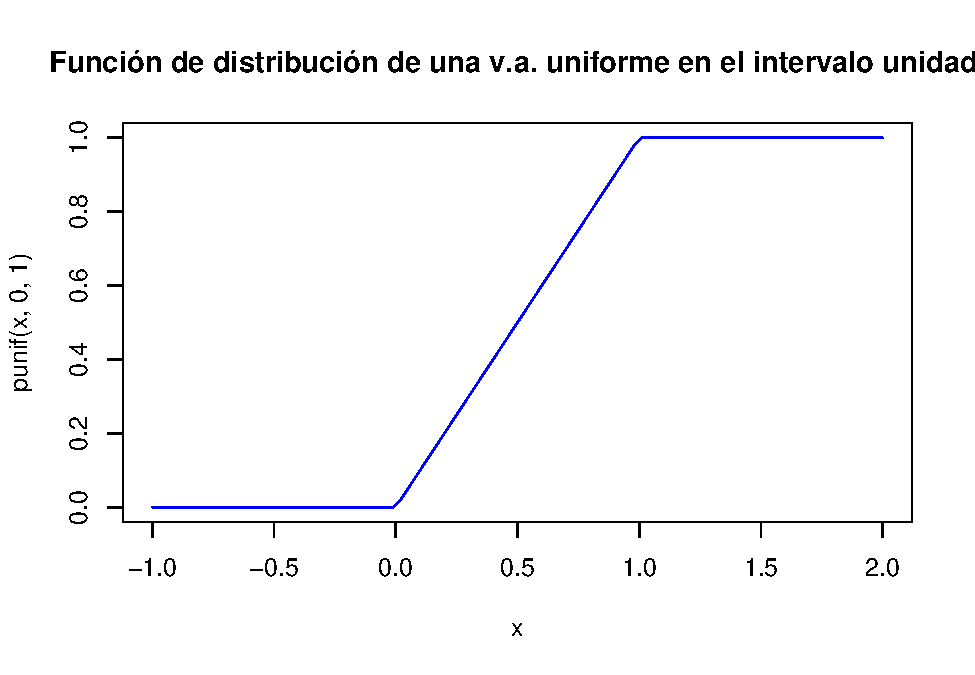
\includegraphics{curso-probabilidad-udemy_files/figure-latex/figUNIF-7} \end{center}

\hypertarget{propiedades-18}{%
\subsection{Propiedades}\label{propiedades-18}}

En las variables continuas los sucesos del tipo \(\{X\leq x \}\) y \(\{X< x \}\) tendrán la
misma probabilidad, y otros tipos de sucesos similares también, algunas de estas
propiedades se explicitan en la siguiente proposición.

Propiedades

Dada una v.a. continua \(X\) se tiene que:

\begin{itemize}
\tightlist
\item
  \(P(X\leq b)=P(X<b)\)
\item
  \(P(X<b)=P(X<a)+P(a<X<b)\)
\item
  \(P(a<X<b)=P(X<b)-P(X<a)\)
\end{itemize}

\hypertarget{demostraciuxf3n-2}{%
\subsection{Demostración}\label{demostraciuxf3n-2}}

\textbf{Demostración:}

La primera es evidente \(P(X\leq b)=P(X<b)+P(X=b)=P(X<b)\)

Para demostrar la segunda, tenemos

\[\{X<a\}\cap \{a<X<b\}=\emptyset\]
\[\{X<a\}\cup \{a<X<b\}=\{X<b\}\]

entonces

\begin{eqnarray*}
P(X\leq b)= & P(\{X<a\}\cup \{a<X<b\})\\
& = P(X<a)+P(a<X<b)
\end{eqnarray*}

\textbf{Ejercicio}

La demostración de la tercera propiedad es similar a la segunda pero aplicando la primera. Queda de ejercicio.

\hypertarget{propiedades-de-la-funciuxf3n-de-distribuciuxf3n-1}{%
\subsection{Propiedades de la función de distribución}\label{propiedades-de-la-funciuxf3n-de-distribuciuxf3n-1}}

Las propiedades anteriores y combinaciones de ellas se pueden
escribir utilizando la función de distribución de \(X\):

 Propiedades de la Función de Distribución

Dada una variable aleatoria continua se tiene que:

\begin{itemize}
\tightlist
\item
  \(F_{X}(b)=F_{X}(a)+P(a<X<b)\)
\item
  \(P(a<X<b)=F_{X}(b)-F_{X}(a)\)
\item
  \(P(a\leq X\leq b)=F_{X}(b)-F_{X}(a)\)
\end{itemize}

\textbf{Ejercicio}

Se deja la demostración como ejercicio

\hypertarget{ejemplo-20}{%
\subsection{Ejemplo}\label{ejemplo-20}}

\textbf{Ejemplo: lanzamiento de dardos}

En los dardos:
\[P(0.25<X<0.3)=F_{X}(0.3)-F_{X}(0.25)=\]
\[=0.3-0.25=0.05\]

\hypertarget{funciuxf3n-de-densidad}{%
\subsection{Función de densidad}\label{funciuxf3n-de-densidad}}

 \textbf{Función de densidad}

Una función \(f:\mathbb{R}\to\mathbb{R}\) es una función de densidad sobre \(\mathbb{R}\) si cumple que

\begin{itemize}
\tightlist
\item
  \(f_{X}(x)\geq 0\) para todo \(x \in\mathbb{R}.\)
\item
  \(f\) es continua salvo a lo más en una cantidad finita de puntos sobre
  cada intervalo acotado de \(\mathbb{R}\).
\item
  \(\displaystyle\int\limits_{-\infty}^{+\infty} f_{X}(x) dx=1.\)
\end{itemize}

\hypertarget{funciuxf3n-de-densidad-de-una-variable-aleatoria.}{%
\subsection{Función de densidad de una variable aleatoria.}\label{funciuxf3n-de-densidad-de-una-variable-aleatoria.}}

 \textbf{Función de densidad de una variable aleatoria}

Sea \(X\) una v.a. con función de distribución \(F_X\). Sea \(f:\mathbb{R}\to\mathbb{R}\) una función de densidad tal que

\[F_X(x)=\displaystyle\int_{-\infty}^{x} f_X(t) dt.\mbox{ para todo } x\in\mathbb{R}.\]

Entonces \(X\) es una variable aleatoria continua y \(f_X\) es la densidad de la v.a. \(X\).

\hypertarget{dominio-de-una-variable-aleatoria-continua}{%
\subsection{Dominio de una variable aleatoria continua}\label{dominio-de-una-variable-aleatoria-continua}}

El conjunto \(D_X=\{x\in\mathbb{R}| f_x(x)>0\}\) recibe el nombre de soporte o dominio de la
variable aleatoria continua y se interpreta su conjunto de resultados posibles.

\textbf{Ejemplo}

En nuestra diana, la función \(f\) es una densidad

\[
f_{X}(x)=\left\{
\begin{array}{ll}
0 & \mbox{si } x\leq 0\\
1 & \mbox{si } 0 < x < 1\\
0 & \mbox{si } 1\leq x
\end{array}\right.
\]

que es la densidad de \(X\), en efecto:

\hypertarget{densidad-diana}{%
\subsection{Densidad diana}\label{densidad-diana}}

\[
f_{X}(x)=\left\{
\begin{array}{ll}
0 & \mbox{si } x\leq 0\\
1 & \mbox{si } 0 < x < 1\\
0 & \mbox{si } 1\leq x
\end{array}\right.
\]

Si \(x \leq 0\) entonces \(\displaystyle\int_{-\infty}^x f_X(t) dt = 0.\)

Si \(0\leq x\leq 1\) entonces \(\displaystyle\int_{-\infty}^x f_X(t) dt = \int_0^x 1 dt = x.\)

Si \(x\geq 1\) entonces \(\displaystyle\int_{-\infty}^x f_X(t) dt = \int_0^1 1 dt = 1.\)

Por lo tanto \(F_X(x)=\displaystyle\int_{-\infty}^x f_X(t) dt\) para todo \(x\in\mathbb{R}.\)

\hypertarget{densidad-diana-1}{%
\subsection{Densidad diana}\label{densidad-diana-1}}

\begin{Shaded}
\begin{Highlighting}[]
\KeywordTok{curve}\NormalTok{(}\KeywordTok{dunif}\NormalTok{(x,}\DecValTok{0}\NormalTok{,}\DecValTok{1}\NormalTok{),}\DataTypeTok{xlim=}\KeywordTok{c}\NormalTok{(}\OperatorTok{-}\FloatTok{0.5}\NormalTok{,}\FloatTok{1.5}\NormalTok{),}\DataTypeTok{col=}\StringTok{"blue"}\NormalTok{,}
      \DataTypeTok{main=}\StringTok{"Densidad de la distribución uniforme en [0,1]"}\NormalTok{)}
\end{Highlighting}
\end{Shaded}

\begin{center}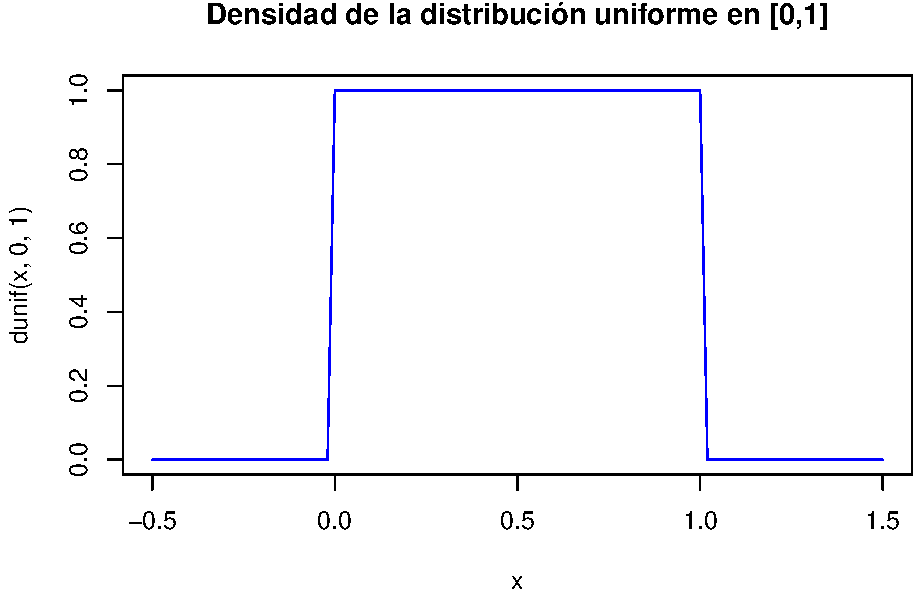
\includegraphics{curso-probabilidad-udemy_files/figure-latex/unnamed-chunk-10-1} \end{center}

\hypertarget{utilidad-de-la-funciuxf3n-de-densidad}{%
\subsection{Utilidad de la función de densidad}\label{utilidad-de-la-funciuxf3n-de-densidad}}

La función de densidad nos permite calcular diversas probabilidades.

Propiedades de la función de densidad

Sea \(X\) una v.a. continua con función de distribución \(F_X\) y de
densidad \(f_X\), entonces

\begin{itemize}
\item
  \begin{eqnarray*}
  P(a< X< b) &=&  P(a<X\leq b)= P(a\leq X< b)=\\
   & & P(a\leq X\leq b)= \displaystyle\int_{a}^b f_X(x) dx.
  \end{eqnarray*}
\item
  Si \(A\) es un conjunto adecuado de \(\mathbb{R}\) entonces
\end{itemize}

\[
P(X\in A)=\displaystyle\int_{A} f(x) dx=\displaystyle\int_{A\cap D_X} f(x) dx.
\]

\hypertarget{utilidad-de-la-funciuxf3n-de-densidad-1}{%
\subsection{Utilidad de la función de densidad}\label{utilidad-de-la-funciuxf3n-de-densidad-1}}

Propiedades de la función de densidad

Sea \(X\) una v.a. continua con función de distribución \(F_X\) y de densidad \(f_X\), entonces:

\begin{itemize}
\tightlist
\item
  Si \(f_x\) es continua en un punto \(x\), \(F_X\) es derivable en ese punto y
  \(F_X'(x)=f_X(x).\)
\item
  \(P(X=x)=0\) para todo \(x\in\mathbb{R}.\)
\end{itemize}

\textbf{Ejercicio}

Comprobar estas propiedades en el ejemplo de la diana.

\hypertarget{ejemplo-tiempo-ejecuciuxf3n-de-un-proceso}{%
\subsection{Ejemplo tiempo ejecución de un proceso}\label{ejemplo-tiempo-ejecuciuxf3n-de-un-proceso}}

\textbf{Ejemplo: Tiempo ejecución de un proceso.}

Sea \(X=\) tiempo de ejecución de un proceso. Se supone que \(X\) sigue una distribución uniforme en dos unidades de tiempo, si tarda más el proceso se cancela.

Calculemos la función de densidad y de distribución de la v.a \(X\).

Entonces

\[
F_{X}(x)=P(X\leq x)=\frac{CF}{CP}=\frac{x}2
\]

Luego su función de distribución es:

\[
F_{X}(x)=\left\{\begin{array}{ll}
0 & \mbox{si } x\leq 0\\
\frac{x}2 & \mbox{si } 0<x<2\\
1 & \mbox{si } 2\leq x
\end{array}\right.
\]

\hypertarget{ejemplo-tiempo-ejecuciuxf3n-de-un-proceso-1}{%
\subsection{Ejemplo tiempo ejecución de un proceso}\label{ejemplo-tiempo-ejecuciuxf3n-de-un-proceso-1}}

Su función de densidad por su lado es:
\[
f_{X}(x)=F_{X}'(x)=\left\{\begin{array}{ll}
0 & \mbox{si } x\leq 0\\
\frac12 & \mbox{si } 0<x\leq 2\\
0 & \mbox{si } 2\leq x
\end{array}\right.
\]

Efectivamente

\begin{itemize}
\tightlist
\item
  \(f_{X}(x)\geq 0,\) y tiene un conjunto finito de discontinuidades.
\item
  \(F_X(x)=\int_{-\infty}^x f_X(t) dt.\) para todo \(x\in \mathbb{R}\) (Ejercicio,
  resolverlo gráficamente.)
\item
  \(\int\limits_{-\infty}^{+\infty}f_{X}(x)dx= \int\limits_0^2\frac12dx=\frac{x}2\mid_0^2= =\frac22-\frac02=1.\)
\end{itemize}

\hypertarget{ejemplo-tiempo-ejecuciuxf3n-de-un-proceso-2}{%
\subsection{Ejemplo tiempo ejecución de un proceso}\label{ejemplo-tiempo-ejecuciuxf3n-de-un-proceso-2}}

\textbf{Ejercicio: Tiempo de un proceso:}

Calcular la probabilidad de que uno de nuestros procesos tarde
más de una unidad de tiempo en ser procesado. Calcular también la probabilidad de
que dure entre \(0.5\) y \(1.5\) unidades de tiempo.

\hypertarget{esperanza-y-varianza-para-variables-aleatorias-continuas}{%
\section{Esperanza y varianza para variables aleatorias continuas}\label{esperanza-y-varianza-para-variables-aleatorias-continuas}}

\hypertarget{esperanza-y-varianza-para-variables-aleatorias-continuas-1}{%
\subsection{Esperanza y varianza para variables aleatorias continuas}\label{esperanza-y-varianza-para-variables-aleatorias-continuas-1}}

Los mismos comentarios y definiciones que se dieron en la sección correspondiente del tema
de estadística descriptiva son aplicables aquí.

Así que sólo daremos las definiciones, la forma de cálculo y algunos ejemplos.

En lo que sigue, salvo que diagamos lo contrario, \(X\) es una v.a. continua con función de densidad \(f_{X}(x)\)

\hypertarget{esperanza-y-varianza-para-variables-aleatorias-continuas-2}{%
\subsection{Esperanza y varianza para variables aleatorias continuas}\label{esperanza-y-varianza-para-variables-aleatorias-continuas-2}}

 Esperanza v.a. continuas

\begin{itemize}
\tightlist
\item
  Su esperanza es:
  \[E(X)=\displaystyle\int\limits_{-\infty}^{+\infty} xf_{X}(x)dx.\]
\item
  Si \(g(x)\) es una función de la variable \(X\) entonces:
  \[E(g(X))=\displaystyle\int\limits_{-\infty}^{+\infty} g(x)\cdot f_{X}(x)dx.\]
\end{itemize}

\hypertarget{esperanza-y-varianza-para-variables-aleatorias-continuas-3}{%
\subsection{Esperanza y varianza para variables aleatorias continuas}\label{esperanza-y-varianza-para-variables-aleatorias-continuas-3}}

 Varianza v.a. continuas

\begin{itemize}
\tightlist
\item
  Su varianza es:
  \[
  Var(X)=\sigma_{X}^2=E((X-\mu_{X})^2)=
  \displaystyle\int\limits_{-\infty}^{+\infty} (x-\mu_{X})^2 f_{X}(x)dx.
  \]
\item
  Su desviación típica es: \[\sigma_{X}=+\sqrt{\sigma_{X}^2}.\]
\end{itemize}

\hypertarget{propiedades-19}{%
\subsection{Propiedades}\label{propiedades-19}}

 Propiedades

\begin{itemize}
\tightlist
\item
  \(\sigma_{X}^2\geq 0\)
\item
  \(Var(cte)=E(cte^2)-(E(cte))^2= cte^2 - cte^2=0\)
\item
  \(Var(x)=E(X^2)-\mu_{X}^2=\int\limits_{-\infty}^{+\infty}x^2 f_{X}(x)dx - \mu_{X}^2.\)
\item
  El mínimo de \(E((X-C)^2)\) se alcanza cuando \(C=E(X)\) y es \(Var(X)\).
\end{itemize}

\hypertarget{ejemplo-21}{%
\subsection{Ejemplo}\label{ejemplo-21}}

\textbf{Ejemplo: Dardo}

Calcular \(\mu_{X}\) y \(\sigma_{X}^2\) en el dardo.

Resultado
\[\mu_{X}=\frac12,\]
\[E(X^2)=\frac13,\]
\[Var(X)=\frac1{12}.\]

\hypertarget{esperanza-de-trasformaciones-lineales-de-v.a.-continuas}{%
\subsection{Esperanza de trasformaciones lineales de v.a. continuas}\label{esperanza-de-trasformaciones-lineales-de-v.a.-continuas}}

 Proposición

Sea \(X\) una v.a. continua con \(E(X)=\mu_{X}\) y \(Var(X)=\sigma_{X}^2\) sea \(Y=a+b X\), donde
\(a,b\in\mathbb{R}\), es una nueva v.a. continua obtenida mediante una transformación lineal de \(X\).
Se verifican las mismas propiedades que en el caso discreto:

\begin{itemize}
\tightlist
\item
  \(E(Y)=E(a+b X)=a+b E(X)\)
\item
  \(Var(Y)=Var(a+b X)=b^2 Var(X)\)
\item
  \(\sigma_{Y}=|b| \sigma_{X}\)
\item
  \(Z=\frac{X-\mu_{X}}{\sigma_{X}}\) es una transformación
  lineal de \(X\) de forma que
  \[E(Z)=0 \mbox{ y } Var(Z)=1\]
\end{itemize}

\hypertarget{ejemplo-22}{%
\subsection{Ejemplo}\label{ejemplo-22}}

\textbf{Ejemplo}

En una empresa de venta de vinos por internet, sea
\(X=\) número de litros de vino del país vendidos en un año.
Supongamos que sabemos que \(E(X)=10000\) y que \(Var(X)=100\)
Supongamos que los gastos fijos de distribución son
50.000 € y el beneficio por litro es de 10 € por botella.
Definimos \(T=10 X-50000\) que será el beneficio después de gastos.

Entonces la esperanza del beneficio es
\[E(T)=10 E(X)-50000 = 50000\]
y
\[Var(T)=10^2 Var(X)= 10000\]

\hypertarget{transformaciones-de-variables-aleatorias}{%
\section{Transformaciones de variables aleatorias}\label{transformaciones-de-variables-aleatorias}}

\hypertarget{transformaciones-de-variables-aleatorias-1}{%
\subsection{Transformaciones de variables aleatorias}\label{transformaciones-de-variables-aleatorias-1}}

Muchas variables aleatorias son funciones de otras v.a. En lo que sigue resumiremos diversas técnicas para dada una v.a. \(X\) y una
transformación \(Y=h(X)\) encontrar \(F_{Y}\) a
partir de \(F_{X}\).

\hypertarget{propiedad}{%
\subsection{Propiedad}\label{propiedad}}

Tranformación de v.a. discretas

Sea \(X\) una v.a. discreta con \(X(\Omega)=\{x_1,x_2,\ldots,x_{n},..\}\) y sea \(h:\mathbb{R}\to\mathbb{R}\) una aplicación.
Entonces \(Y=h(X)\) es también una v.a. discreta. Además si \(P_X\)
y \(F_{X}\) son las funciones de probabilidad y de distribución de
\(X\) entonces

\begin{itemize}
\tightlist
\item
  \(\displaystyle P_{Y}(y)=\sum_{x_{i}|h(x_{i})=y}P_X(x_{i}).\)
\item
  \(\displaystyle F_{Y}(y)=\sum_{x_{i}|h(x_{i})\leq y} P_X(x_{i}).\)
\end{itemize}

\hypertarget{propiedades-20}{%
\subsection{Propiedades}\label{propiedades-20}}

Desafortunadamente para variables no discetas el asunto no es tan sencillo como el anterior, pues la transformación de, por ejemplo, una v.a. continua puede ser continua, discreta, mixta\ldots{}

Transformación de v.a. continuas en continuas

Sea \(X\) una v.a. continua cuya función de densidad es \(f_{X}\). Sea
\(h:\mathbb{R}\to\mathbb{R}\) una aplicación estrictamente monótona y derivable, tal
que \(h'(x)\not=0\) para todo \(x\in\mathbb{R}\). Sea \(Y=h(X)\) la
transformación de \(X\) por \(h\). Entonces \(Y\) es una v.a. continua con función
de densidad

\[f_{Y}(y)=\left.\frac{f_{X}(x)}
{\left|h'(x)\right|}\right|_{x=h^{-1}(y)}\]

\hypertarget{propiedades-21}{%
\subsection{Propiedades}\label{propiedades-21}}

 Densidad de una transformación de una v.a. continua

Sea \(X\) una v.a. continua cuya función de densidad es \(f_{X}\). Sea
\[h:\mathbb{R}\to\mathbb{R}\]
una aplicación, no necesariamente monótona tal que :

\begin{itemize}
\tightlist
\item
  sea derivable con derivada no nula
\item
  la ecuación \(h(x)=y\) tiene un número finito de soluciones
  \(x_1,x_2,..,x_{n}\)
\end{itemize}

entonces:

\[
\displaystyle f_{Y}(y)=\left.\sum_{k=1}^{n} \frac{f_{X}(x)}
{\left|h'(x)\right|}\right|_{x=x_{k}}.
\]

\hypertarget{muxe9todo-general-del-transformaciuxf3n-de-v.a.}{%
\subsection{Método general del transformación de v.a.}\label{muxe9todo-general-del-transformaciuxf3n-de-v.a.}}

Cuando no podamos aplicar las propiedades anteriores intentaremos
calcular primero la función de distribución de la transformación
y luego su densidad.

Notemos que en general si \(Y=g(X)\) es una v.a. transformación de la
v.a. \(X\) entonces

\[
F_{Y}(y)=P(Y\leq y)=P(g(X)\leq y).
\]

\hypertarget{muxe9todo-general-del-transformaciuxf3n-de-variables-aleatorias}{%
\subsection{Método general del transformación de variables aleatorias}\label{muxe9todo-general-del-transformaciuxf3n-de-variables-aleatorias}}

Por ejemplo si \(g\) es estrictamente creciente y cont.

\[
F_{Y}(y)=P(g(X)\leq y)=P(X\leq g^{-1}(y))=F_{X}(g^{-1}(y)).
\]

y si \(g\) es estrictamente decreciente y cont.
\[
F_{Y}(y)=P(g(X)\leq y)=P(X\geq g^{-1}(y))=1-F_{X}(g^{-1}(y)).
\]

\hypertarget{desigualdades-buxe1sicas-markov-y-chebychev}{%
\section{Desigualdades básicas: Markov y Chebychev}\label{desigualdades-buxe1sicas-markov-y-chebychev}}

\hypertarget{desigualdades-de-markov-y-de-chebychev}{%
\subsection{Desigualdades de Markov y de Chebychev}\label{desigualdades-de-markov-y-de-chebychev}}

\begin{itemize}
\tightlist
\item
  En esta sección distintas desigualdades que acotan determinadas probabilidades de
  una variable aleatoria.
\item
  Estas desigualdades sirven en algunos casos para acotar probabilidades de determinados sucesos.
\item
  También son útiles desde el punto de vista teórico, por ejemplo para justificar que la varianza es una mediada de la dispersión de
  los datos.
\end{itemize}

\hypertarget{desigualdad-de-markov}{%
\subsection{Desigualdad de Markov}\label{desigualdad-de-markov}}

 Desigualdad de Markov

Sea \(X\) una v.a. positiva con \(E(X)\) finita. Entonces

\[P(X\geq a)\leq \frac{E(X)}{a}\mbox{ para todo }a>0.\]

\textbf{Demostración}:

Si \(X\) es continua y solo toma valores positivos

\begin{eqnarray*}
E(X) &=& \int_{-\infty}^{+\infty} x f_{X}(x) dx=  \int_0^{+\infty} x f_{X}(x) dx=  \int_0^{a} x f_{X}(x) dx +\int_{a}^{+\infty} x f_{X}(x) dx \\
& &\geq   \int_{a}^{+\infty} x
f_{X}(x) dx \geq a \int_{a}^{+\infty}
f_{X}(x) dx = a \cdot  P(X\geq a)
\end{eqnarray*}.

de donde se sigue que

\[P(X\geq a)\leq \frac{E(X)}{a}.\]

\hypertarget{desigualdad-de-markov-1}{%
\subsection{Desigualdad de Markov}\label{desigualdad-de-markov-1}}

 Corolario

Sea \(X\) una v.a. con \(E(X)\) finita entonces para todo \(a>0\)

\[P(|X|\geq a )\leq \frac{E(|X|)}{a}.\]

\textbf{Ejercicio}

Demuestra el corolario anterior a partir de la desigualdad de Markov.

\hypertarget{desigualdad-de-chebychev}{%
\subsection{Desigualdad de Chebychev}\label{desigualdad-de-chebychev}}

La desigualdad de Chebychev también se denomina de Chebyshov y en inglés Chebyshev.

 Desigualdad de Chebychev

Sea \(X\) una v.a.con \(E(X)=\mu\) y \(Var(X)=\sigma^2\) entonces para todo \(a>0\)

\[P(|X-\mu|\geq a)\leq \frac{\sigma^2}{a^2}\]

\hypertarget{demostraciuxf3n-desigualdad-de-chebychev}{%
\subsection{Demostración desigualdad de Chebychev}\label{demostraciuxf3n-desigualdad-de-chebychev}}

\textbf{Demostración}

Apliquemos la consecuencia de la desigualdad de Markov a la v.a.
no negativa

\[Y^2=(X-\mu)^2\]

entonces

\[
P(Y^2\geq a^2) \leq 
\frac{E(Y^2)}{a^2}=\frac{E((X-\mu)^2)}{a^2}
= \frac{Var(X)}{a^2}=\frac{\sigma^2}{a^2}
.
\]

Por otra parte

\[
P(Y^2\geq a^2)=P(|Y|\geq a)= P(|X-\mu|\geq a).
\]

hecho que, junto con la desigualdad anterior,
demuestra el resultado.

\hypertarget{uso-de-la-desigualdad-de-chebychev}{%
\subsection{Uso de la desigualdad de Chebychev}\label{uso-de-la-desigualdad-de-chebychev}}

 \textbf{Utilidad básica de la desigualdad de Chebychev}

Supongamos que \(X\) es una v.a. con \(Var(X)=0\)
entonces.

Aplicando la desigualdad anterior

\[P(|X-E(X)|\geq a )=0\mbox{ para todo }a>0\]
lo que implica que

\[P(X=E(X))=1.\]

Por lo que probabilidad de que \(X\) sea
constantemente \(E(X)\) es 1.

Lo que nos confirma la utilidad de la varianza es una
medida de la dispersión de los datos.

\hypertarget{ejemplo-23}{%
\subsection{Ejemplo}\label{ejemplo-23}}

\textbf{Ejemplo}

Se sabe que el tiempo de respuesta medio y la desviación típica de un sistema multiusuario son 15 y 3 u.t.respectivamente. Entonces:

\[
P(|X-15|\geq 5)\leq \frac9{25}=0.36.
\]

Si substituimos \(a\) por \(a\cdot \sigma\) en la
desigualdad de Chebychev, nos queda:

\[
P(|X-\mu|\geq a \sigma)\leq
\frac{\sigma^2}{(a\sigma)^2}=\frac1{a^2}.
\]

Que es otra manera de expresar la desigualdad de Chebychev.

\hypertarget{muxe1s-formas-de-la-desgualdad-de-chebychev}{%
\subsection{Más formas de la desgualdad de Chebychev}\label{muxe1s-formas-de-la-desgualdad-de-chebychev}}

La desigualdad de Chebychev también se puede escribir de al menos dos maneras más:

\[
P(\mu-a\leq X\leq \mu+a)\geq 1-\frac{\sigma^2}{a^2}
\]

y tomado como \(a=k\cdot \sigma\)

\[
P(\mu-k\cdot \sigma\leq X\leq \mu+ k \cdot \sigma)\geq 1-\frac1{k^2}
\]

\hypertarget{la-varianza-como-medida-de-dispersiuxf3n}{%
\subsection{La varianza como medida de dispersión}\label{la-varianza-como-medida-de-dispersiuxf3n}}

Tomando la segunda expresión que hemos visto para la desigualdad de
Chebychev para distintos valores de \(k>0\) tenemos la siguiente tabla.

\begin{longtable}[]{@{}ll@{}}
\toprule
k & \(P(|X-E(X)|\geq k \cdot \sigma)\)\tabularnewline
\midrule
\endhead
1 & \(\leq 1\)\tabularnewline
2 & \(\leq 0.25\)\tabularnewline
3 & \(\leq 0.111\)\tabularnewline
4 & \(\leq 0.0025\)\tabularnewline
\bottomrule
\end{longtable}

\hypertarget{interpretaciuxf3n-de-la-desigualdad}{%
\subsection{Interpretación de la desigualdad}\label{interpretaciuxf3n-de-la-desigualdad}}

\begin{itemize}
\item
  Por ejemplo para \(k=2\) esta desigualdad se puede interpretar como que dada una v.a. \(X\) con cualquier distribución que tenga \(E(X)\) y \(Var(X)\) finitos \emph{la probabilidad de que un valor se aleje de la media \(\mu\) más de \(a=2\) desviaciones típicas es menor o igual que \(0.25\)}.
\item
  Es decir sólo el 25\% de los valores estarán alejados de la media
  más de \(2\sigma\)
\end{itemize}

¡\emph{Sea cual sea la distribución de la v.a.}!

\hypertarget{distribuciones-notables}{%
\chapter{Distribuciones Notables}\label{distribuciones-notables}}

\begin{itemize}
\item
  En este tema estudiaremos diversos tipos de experimentos que son muy frecuentes y algunas de las variables aleatorias asociadas a ellos.
\item
  Estas variables reciben distintos nombres que aplicaremos sin distinción al tipo de población del experimento a la variable o a su función de probabilidad, densidad o distribución.
\item
  Empezaremos con las variables aleatorias discretas que se presentan con frecuencia ya que están relacionadas con situaciones muy comunes como el número de caras en varios lanzamiento de una moneda, el número de veces que una maquina funciona hasta que se estropea, el numero de clientes en una cola,\ldots{}
\end{itemize}

\hypertarget{distribuciuxf3n-bernoulli}{%
\section{Distribución Bernoulli}\label{distribuciuxf3n-bernoulli}}

 Distribución Bernoulli

\begin{itemize}
\tightlist
\item
  Consideremos un experimento con dos resultados posibles éxito (E) y
  fracaso (F). El espacio de sucesos será \(\Omega=\{E,F\}\).
\item
  Supongamos que la probabilidad de éxito es \(P(E)=p\), y naturalmente \(P(F)=1-p=q\) con \(0<p<1\).
\item
  Consideremos la aplicación
\end{itemize}

\[
X:\Omega=\{E,F\}\to \mathbb{R}
\]

definida por

\[
X(E)=1\mbox{, }X(F)=0.
\]

Su función de probabilidad es

\[
P_{X}(x)=
\left\{
\begin{array}{ll} 1-p=q & \mbox{si } x=0\\
p & \mbox{si } x=1\\
0 & \mbox{en cualquier otro caso}
\end{array}
\right..
\]

Su función de distribución es

\[
F_{X}(x)=P(X\leq x)=
\left\{
\begin{array}{ll} 
0 & \mbox{si } x<0\\
1-p=q & \mbox{si } 0\leq x <1\\
1 & \mbox{si } 1\leq x \\
\end{array}
\right..
\]

\begin{itemize}
\tightlist
\item
  Bajo estas condiciones diremos que \(X\) \textbf{es una v.a. Bernoulli} o que sigue una ley de \textbf{distribución de probabilidad Bernoulli} de parámetro \(p\).
\item
  Lo denotaremos por
  \[X\equiv Ber(p)\mbox{ o también } X\equiv B(1,p).\]
\item
  A este tipo de experimentos (éxito/fracaso)se les denomina experimentos Bernoulli.
\item
  Fue su descubridor un científico suizo \href{https://es.wikipedia.org/wiki/Jakob_Bernoulli}{Jacob Bernoulli}, uno más de la de la conocida \href{https://es.wikipedia.org/wiki/Familia_Bernoulli}{familia de científicos suizos Bernoulli}
\end{itemize}

\hypertarget{esperanza-de-una-v.a.-x-berp}{%
\subsection{\texorpdfstring{Esperanza de una v.a. \(X\) \(Ber(p)\)}{Esperanza de una v.a. X Ber(p)}}\label{esperanza-de-una-v.a.-x-berp}}

Su \textbf{valor esperado} es

\[E(X)=\displaystyle\sum_{x=0}^1 x\cdot P(X=x)= 0\cdot(1-p)+1\cdot p=p.\]

Calculemos también \(E(X^2)\)

\[E(X^2)=\displaystyle\sum_{x=0}^1 x^2\cdot P(X=x)= 0^2\cdot(1-p)+1^2\cdot p=p.\]

\hypertarget{varianza-de-una-v.a.-x-berp}{%
\subsection{\texorpdfstring{Varianza de una v.a. \(X\) \(Ber(p)\)}{Varianza de una v.a. X Ber(p)}}\label{varianza-de-una-v.a.-x-berp}}

Su \textbf{varianza} es

\[Var(X)=E(X^2)-\left(E(X)\right)^2=p-p^2=p\cdot (1-p)=p\cdot q.\]

Su desviación típica es

\[
\sqrt{Var(X)}=\sqrt{p \cdot (1-p)}.
\]

\hypertarget{resumen-v.a-con-distribuciuxf3n-bernoulli}{%
\subsection{Resumen v.a con distribución Bernoulli}\label{resumen-v.a-con-distribuciuxf3n-bernoulli}}

\begin{longtable}[]{@{}rl@{}}
\toprule
\begin{minipage}[b]{0.52\columnwidth}\raggedleft
\(X\) Bernoulli\strut
\end{minipage} & \begin{minipage}[b]{0.42\columnwidth}\raggedright
\(Ber(p)\)\strut
\end{minipage}\tabularnewline
\midrule
\endhead
\begin{minipage}[t]{0.52\columnwidth}\raggedleft
\(D_X=\)\strut
\end{minipage} & \begin{minipage}[t]{0.42\columnwidth}\raggedright
\(\{0,1\}\)\strut
\end{minipage}\tabularnewline
\begin{minipage}[t]{0.52\columnwidth}\raggedleft
\(P_X(x)=P(X=x)=\)\strut
\end{minipage} & \begin{minipage}[t]{0.42\columnwidth}\raggedright
\(\left\{\begin{array}{ll} q & \mbox{si } x=0\\ p & \mbox{si } x=1\\0 & \mbox{en otro caso}\end{array}\right.\)\strut
\end{minipage}\tabularnewline
\begin{minipage}[t]{0.52\columnwidth}\raggedleft
\(F_X(x)=P(X\leq X)=\)\strut
\end{minipage} & \begin{minipage}[t]{0.42\columnwidth}\raggedright
\(\left\{\begin{array}{ll} 0 & \mbox{ si } x<0\\q & \mbox{ si } 0\leq x<1\\1 & \mbox{ si } 1\leq x \end{array}\right.\)\strut
\end{minipage}\tabularnewline
\begin{minipage}[t]{0.52\columnwidth}\raggedleft
\(E(X)=p\)\strut
\end{minipage} & \begin{minipage}[t]{0.42\columnwidth}\raggedright
\(Var(X)=p\cdot q\)\strut
\end{minipage}\tabularnewline
\bottomrule
\end{longtable}

\hypertarget{distribuciuxf3n-bernoulli.-ejemplo}{%
\subsection{Distribución Bernoulli. Ejemplo}\label{distribuciuxf3n-bernoulli.-ejemplo}}

Veamos los cálculos básicos \(Ber(p=0.25)\) en \texttt{R}.

\begin{Shaded}
\begin{Highlighting}[]
\KeywordTok{dbinom}\NormalTok{(}\DecValTok{0}\NormalTok{,}\DataTypeTok{size=}\DecValTok{1}\NormalTok{,}\DataTypeTok{prob=}\FloatTok{0.25}\NormalTok{)}
\end{Highlighting}
\end{Shaded}

\begin{verbatim}
## [1] 0.75
\end{verbatim}

\begin{Shaded}
\begin{Highlighting}[]
\KeywordTok{dbinom}\NormalTok{(}\DecValTok{1}\NormalTok{,}\DataTypeTok{size=}\DecValTok{1}\NormalTok{,}\DataTypeTok{prob=}\FloatTok{0.25}\NormalTok{)}
\end{Highlighting}
\end{Shaded}

\begin{verbatim}
## [1] 0.25
\end{verbatim}

\begin{Shaded}
\begin{Highlighting}[]
\KeywordTok{rbinom}\NormalTok{(}\DataTypeTok{n=}\DecValTok{20}\NormalTok{,}\DataTypeTok{size =} \DecValTok{1}\NormalTok{,}\DataTypeTok{prob=}\FloatTok{0.25}\NormalTok{)}
\end{Highlighting}
\end{Shaded}

\begin{verbatim}
##  [1] 0 0 0 0 0 0 0 0 0 0 0 0 1 1 0 0 1 1 0 0
\end{verbatim}

\hypertarget{distribuciuxf3n-bernoulli.-ejemplo-1}{%
\subsection{Distribución Bernoulli. Ejemplo}\label{distribuciuxf3n-bernoulli.-ejemplo-1}}

El siguiente código dibuja las función de probabilidad y la de distribución de una \(Ber(p=0.25)\)

\begin{Shaded}
\begin{Highlighting}[]
\KeywordTok{par}\NormalTok{(}\DataTypeTok{mfrow=}\KeywordTok{c}\NormalTok{(}\DecValTok{1}\NormalTok{,}\DecValTok{2}\NormalTok{))}
\KeywordTok{plot}\NormalTok{(}\DataTypeTok{x=}\KeywordTok{c}\NormalTok{(}\DecValTok{0}\NormalTok{,}\DecValTok{1}\NormalTok{),}\DataTypeTok{y=}\KeywordTok{dbinom}\NormalTok{(}\KeywordTok{c}\NormalTok{(}\DecValTok{0}\NormalTok{,}\DecValTok{1}\NormalTok{),}\DataTypeTok{size=}\DecValTok{1}\NormalTok{,}\DataTypeTok{prob=}\FloatTok{0.25}\NormalTok{),}
     \DataTypeTok{ylim=}\KeywordTok{c}\NormalTok{(}\DecValTok{0}\NormalTok{,}\DecValTok{1}\NormalTok{),}\DataTypeTok{xlim=}\KeywordTok{c}\NormalTok{(}\OperatorTok{-}\DecValTok{1}\NormalTok{,}\DecValTok{2}\NormalTok{),}\DataTypeTok{xlab=}\StringTok{"x"}\NormalTok{,}
     \DataTypeTok{main=}\StringTok{"Función de probabilidad}\CharTok{\textbackslash{}n}\StringTok{ Ber(p=0.25)"}\NormalTok{)}
\KeywordTok{lines}\NormalTok{(}\DataTypeTok{x=}\KeywordTok{c}\NormalTok{(}\DecValTok{0}\NormalTok{,}\DecValTok{0}\NormalTok{,}\DecValTok{1}\NormalTok{,}\DecValTok{1}\NormalTok{),}\DataTypeTok{y=}\KeywordTok{c}\NormalTok{(}\DecValTok{0}\NormalTok{,}\FloatTok{0.75}\NormalTok{,}\DecValTok{0}\NormalTok{,}\FloatTok{0.25}\NormalTok{), }\DataTypeTok{type =} \StringTok{"h"}\NormalTok{, }\DataTypeTok{lty =} \DecValTok{2}\NormalTok{,}\DataTypeTok{col=}\StringTok{"blue"}\NormalTok{)}
\KeywordTok{curve}\NormalTok{(}\KeywordTok{pbinom}\NormalTok{(x,}\DataTypeTok{size=}\DecValTok{1}\NormalTok{,}\DataTypeTok{prob=}\FloatTok{0.25}\NormalTok{),}
      \DataTypeTok{xlim=}\KeywordTok{c}\NormalTok{(}\OperatorTok{-}\DecValTok{1}\NormalTok{,}\DecValTok{2}\NormalTok{),}\DataTypeTok{col=}\StringTok{"blue"}\NormalTok{,}
      \DataTypeTok{main=}\StringTok{"Función de distribución\textbackslash{}n Ber(p=0.25)"}\NormalTok{)}
\KeywordTok{par}\NormalTok{(}\DataTypeTok{mfrow=}\KeywordTok{c}\NormalTok{(}\DecValTok{1}\NormalTok{,}\DecValTok{1}\NormalTok{))}
\end{Highlighting}
\end{Shaded}

\hypertarget{distribuciuxf3n-bernoulli.-ejemplo-2}{%
\subsection{Distribución Bernoulli. Ejemplo}\label{distribuciuxf3n-bernoulli.-ejemplo-2}}

\begin{center}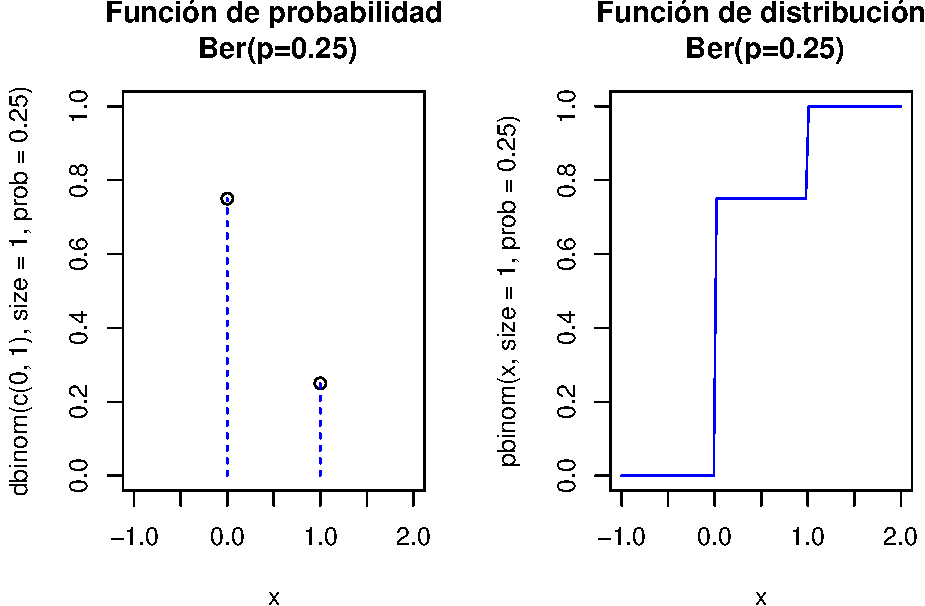
\includegraphics{curso-probabilidad-udemy_files/figure-latex/unnamed-chunk-12-1} \end{center}

\hypertarget{gruxe1ficas-interactivas-berp}{%
\subsection{\texorpdfstring{Gráficas interactivas \(Ber(p)\)}{Gráficas interactivas Ber(p)}}\label{gruxe1ficas-interactivas-berp}}

Para ejecutar el siguiente gráfico interactivo, solamente tienes que cargar el paquete \texttt{shiny} en tu ordenador y luego copiar/pegar las siguientes instrucciones. De este modo podrás observar los cambios en las distribuciones variando los parámetros.

\begin{Shaded}
\begin{Highlighting}[]
\KeywordTok{sliderInput}\NormalTok{(}\StringTok{"p_ber"}\NormalTok{, }\DataTypeTok{label =} \StringTok{"Probabilidad éxito p:"}\NormalTok{,}
              \DataTypeTok{min =} \FloatTok{0.01}\NormalTok{, }\DataTypeTok{max =} \FloatTok{0.99}\NormalTok{, }\DataTypeTok{value =} \FloatTok{0.25}\NormalTok{, }\DataTypeTok{step =} \FloatTok{0.01}\NormalTok{)}

\KeywordTok{renderPlot}\NormalTok{(\{}
\KeywordTok{par}\NormalTok{(}\DataTypeTok{mfrow=}\KeywordTok{c}\NormalTok{(}\DecValTok{1}\NormalTok{,}\DecValTok{2}\NormalTok{))}
\NormalTok{  p=input}\OperatorTok{$}\NormalTok{p_ber}
\KeywordTok{plot}\NormalTok{(}\DataTypeTok{x=}\KeywordTok{c}\NormalTok{(}\DecValTok{0}\NormalTok{,}\DecValTok{1}\NormalTok{),}\DataTypeTok{y=}\KeywordTok{dbinom}\NormalTok{(}\KeywordTok{c}\NormalTok{(}\DecValTok{0}\NormalTok{,}\DecValTok{1}\NormalTok{),}\DataTypeTok{size=}\DecValTok{1}\NormalTok{,}\DataTypeTok{prob=}\NormalTok{p),}
     \DataTypeTok{ylim=}\KeywordTok{c}\NormalTok{(}\DecValTok{0}\NormalTok{,}\DecValTok{1}\NormalTok{),}\DataTypeTok{xlim=}\KeywordTok{c}\NormalTok{(}\OperatorTok{-}\FloatTok{0.5}\NormalTok{,}\DecValTok{2}\NormalTok{),}\DataTypeTok{xlab=}\StringTok{"x"}\NormalTok{,}\DataTypeTok{pch=}\DecValTok{21}\NormalTok{,}
     \DataTypeTok{main=}\KeywordTok{paste0}\NormalTok{(}\KeywordTok{c}\NormalTok{(}\StringTok{"Función de probabilidad}\CharTok{\textbackslash{}n}
\StringTok{                   Ber(p="}\NormalTok{,p,}\StringTok{")"}\NormalTok{),}\DataTypeTok{collapse=}\StringTok{""}\NormalTok{),}\DataTypeTok{bg=}\StringTok{"black"}\NormalTok{)}
\KeywordTok{segments}\NormalTok{(}\DataTypeTok{x0=}\DecValTok{0}\NormalTok{,}\DataTypeTok{y0=}\DecValTok{0}\NormalTok{,}\DataTypeTok{x1=}\DecValTok{0}\NormalTok{,}\DataTypeTok{y1=}\DecValTok{1}\OperatorTok{-}\NormalTok{p, }\DataTypeTok{col =} \StringTok{"blue"}\NormalTok{, }\DataTypeTok{lty =}\DecValTok{2}\NormalTok{)}
\KeywordTok{segments}\NormalTok{(}\DataTypeTok{x0=}\DecValTok{1}\NormalTok{,}\DataTypeTok{y0=}\DecValTok{0}\NormalTok{,}\DataTypeTok{x1=}\DecValTok{1}\NormalTok{,}\DataTypeTok{y1=}\NormalTok{p, }\DataTypeTok{col =} \StringTok{"blue"}\NormalTok{, }\DataTypeTok{lty =}\DecValTok{2}\NormalTok{)}
\KeywordTok{segments}\NormalTok{(}\DataTypeTok{x0=}\OperatorTok{-}\DecValTok{1}\NormalTok{,}\DataTypeTok{y0=}\DecValTok{1}\OperatorTok{-}\NormalTok{p,}\DataTypeTok{x1=}\DecValTok{0}\NormalTok{,}\DataTypeTok{y1=}\DecValTok{1}\OperatorTok{-}\NormalTok{p, }\DataTypeTok{col =} \StringTok{"blue"}\NormalTok{, }\DataTypeTok{lty =}\DecValTok{2}\NormalTok{)}
\KeywordTok{segments}\NormalTok{(}\DataTypeTok{x0=}\OperatorTok{-}\DecValTok{1}\NormalTok{,}\DataTypeTok{y0=}\NormalTok{p,}\DataTypeTok{x1=}\DecValTok{1}\NormalTok{,}\DataTypeTok{y1=}\NormalTok{p, }\DataTypeTok{col =} \StringTok{"blue"}\NormalTok{, }\DataTypeTok{lty =}\DecValTok{2}\NormalTok{)}
\NormalTok{x=}\DecValTok{0}\OperatorTok{:}\DecValTok{1}
\NormalTok{y=}\KeywordTok{pbinom}\NormalTok{(x,}\DataTypeTok{size=}\DecValTok{1}\NormalTok{,}\DataTypeTok{prob=}\NormalTok{p)}
\KeywordTok{curve}\NormalTok{(}\KeywordTok{pbinom}\NormalTok{(x,}\DataTypeTok{size=}\DecValTok{1}\NormalTok{,}\DataTypeTok{prob=}\NormalTok{p),}
      \DataTypeTok{xlim=}\KeywordTok{c}\NormalTok{(}\OperatorTok{-}\DecValTok{1}\NormalTok{,}\DecValTok{2}\NormalTok{),}\DataTypeTok{col=}\StringTok{"blue"}\NormalTok{,}
      \DataTypeTok{main=}\KeywordTok{paste0}\NormalTok{(}\KeywordTok{c}\NormalTok{(}\StringTok{"Función de distribución\textbackslash{}n Ber(p="}\NormalTok{,p,}\StringTok{")"}\NormalTok{),}\DataTypeTok{collapse=}\StringTok{""}\NormalTok{)}
\NormalTok{      )}

\KeywordTok{par}\NormalTok{(}\DataTypeTok{mfrow=}\KeywordTok{c}\NormalTok{(}\DecValTok{1}\NormalTok{,}\DecValTok{1}\NormalTok{))}
\NormalTok{\})}
\end{Highlighting}
\end{Shaded}

\hypertarget{distribuciuxf3n-binomial}{%
\section{Distribución binomial}\label{distribuciuxf3n-binomial}}

 Distribución binomial

Si repetimos \(n\) veces de forma independiente un experimento Bernoulli de parámetro \(p\).

El espacio muestral \(\Omega\) estará formado por cadenas de \(E\)'s y \(F\)'s de longitud \(n\)
Consideremos la v.a.

\[X(\overbrace{EFFF\ldots EEF}^{n})=\mbox{número de éxitos en la cadena}.\]

\hypertarget{funciuxf3n-de-probabilidad-de-una-binomial}{%
\subsection{Función de probabilidad de una binomial}\label{funciuxf3n-de-probabilidad-de-una-binomial}}

Entonces su \textbf{función de probabilidad} es

\[
P_{X}(x)=\left\{
\begin{array}{ll}
{n\choose x}\cdot  p^x \cdot(1-p)^{n-x} &\mbox{ si } x=0,1,\ldots,n\\
0  & \mbox{ en otro caso}
\end{array}\right..
\]

\hypertarget{funciuxf3n-de-distribuciuxf3n-de-binomial}{%
\subsection{Función de distribución de binomial}\label{funciuxf3n-de-distribuciuxf3n-de-binomial}}

Su \textbf{función de distribución} no tiene una fórmula cerrada. Hay que acumular la función de probabilidad:

\[
\begin{eqnarray*}
F_{X}(x)=P(X\leq x) & = & \sum_{i=0}^x P_X(i)\\
& = & 
\left\{
\begin{array}{ll}
0 & \mbox{ si } x\leq 0\\\displaystyle
\sum_{i=0}^k {n\choose i}\cdot  p^i \cdot (1-p)^{n-i} & \mbox{ si } 
\left\{
  \begin{array}{l} 
  k\leq x< k+1\\
  k=0,1,\ldots,n.
  \end{array}
\right.\\
1 & \mbox{ si } n\leq x
\end{array}
\right..
\end{eqnarray*}
\]

\hypertarget{nuxfameros-binomiales-con-r}{%
\subsection{Números binomiales con R}\label{nuxfameros-binomiales-con-r}}

Los números binomiales alculan el número de equipos de baloncestodistintos que (\(k=5\) jugadores) se pueden hacer con 6 jugadores (\(n=6\)).

Es decir cuántas manearas distintas hay para elegir (\emph{choose}) 5 jugadores en un conjunto de 6 jugadores. Todo el mundo diría
¡¡¡6!!!. Efectivamente con R es

\begin{Shaded}
\begin{Highlighting}[]
\KeywordTok{choose}\NormalTok{(}\DecValTok{6}\NormalTok{,}\DecValTok{5}\NormalTok{)}
\end{Highlighting}
\end{Shaded}

\begin{verbatim}
## [1] 6
\end{verbatim}

Con 10 jugadores el número de equipos de 5 distintos es bastante más grande

\begin{Shaded}
\begin{Highlighting}[]
\KeywordTok{choose}\NormalTok{(}\DecValTok{10}\NormalTok{,}\DecValTok{5}\NormalTok{)}
\end{Highlighting}
\end{Shaded}

\begin{verbatim}
## [1] 252
\end{verbatim}

Y por ejemplo con un equipo de fútbol profesional que tiene en plantilla 22 jugadores (quitando los guardametas) se pueden formar ¡¡nada menos que!!

\begin{Shaded}
\begin{Highlighting}[]
\KeywordTok{choose}\NormalTok{(}\DecValTok{22}\NormalTok{,}\DecValTok{10}\NormalTok{)}
\end{Highlighting}
\end{Shaded}

\begin{verbatim}
## [1] 646646
\end{verbatim}

un bonito número capicúa que nos da el número de equipos distintos que se pueden formar.

\hypertarget{distribuciuxf3n-binomial-1}{%
\subsection{Distribución Binomial}\label{distribuciuxf3n-binomial-1}}

En las anteriores circunstancias diremos que la v.a. sigue una \textbf{ley de probabilidad binomial} \ldots{} con parámetros \(n\) y \(p\) y lo denotaremos así

\[X\equiv B(n,p).\]

Obviamente se tiene que una bernoulli es una binomial con \(n=1\)

\[B(1,p)=Ber(p).\]

\textbf{Ejercicio}

Calculad las funciones de distribución de una binomial \(B(n=1,p=0.3)\) y comprobar que coinciden con las distribuciones de una \(Ber(p=0.3)\).

\hypertarget{observaciones-sobre-la-distribuciuxf3n-binomial}{%
\subsection{Observaciones sobre la distribución binomial}\label{observaciones-sobre-la-distribuciuxf3n-binomial}}

\begin{itemize}
\tightlist
\item
  La probabilidad de fracaso se suele denotar con \(q=1-p\), \textbf{sin ningún aviso adicional}, con el fin de acortar y agilizar la escritura de las fórmulas.
\item
  Su \textbf{función de distribución no tienen una formula general}, hay que calcularla con una función de R o python\ldots{} En el siglo pasado se tabulaban en los libros de papel :-).
\item
  En el material adicional os pondremos unas tablas de esta distribución
  para distintos valores de \(n\) y \(p\) para que disfrutéis de tan ancestral método de cálculo.
\item
  Cualquier paquete estadístico, hoja de cálculo dispone de
  funciones para el cálculo de estas probabilidades, así que el \textbf{uso de las tablas} queda \textbf{totalmente anticuado}.
\end{itemize}

\hypertarget{esperanza-de-una-x-bnp}{%
\subsection{\texorpdfstring{Esperanza de una \(X\) \(B(n,p)\)}{Esperanza de una X B(n,p)}}\label{esperanza-de-una-x-bnp}}

Su \textbf{esperanza} es
\[E(X)=\displaystyle\sum_{k=0}^n k \cdot  {n \choose k }\cdot p^k\cdot q^{n-k} = n\cdot p.\]

La esperanza de \(X^2\) es

\[
\begin{eqnarray*}
E(X^2)&=& \displaystyle\sum_{k=0}^n k^2 \cdot  {n \choose k }\cdot p^k\cdot q^{n-k}\\
&=& n\cdot p\cdot q-(n\cdot p)^2.
\end{eqnarray*}
\]

\hypertarget{varianza-de-una-x-bnp}{%
\subsection{\texorpdfstring{Varianza de una \(X\) \(B(n,p)\)}{Varianza de una X B(n,p)}}\label{varianza-de-una-x-bnp}}

Su \textbf{varianza} es

\[Var(X)=E(X^2)-\left(E(X)\right)^2=n\cdot p \cdot q=n\cdot p\cdot (1-p).\]

Su desviación típica es

\[\sqrt{n\cdot p\cdot q}=\sqrt{n\cdot p\cdot (1-p)}.\]

En otos temas veremos una forma sencilla del cálculo de la esperanza y varianza de una \(B(n,p)\) como las suma de n \(Ber(p)\) independientes.

\textbf{Ejercicio}

Justificar de forma intuitiva que si \(X_i\) con \(i=1,2,\ldots, n\) son v.a. \(Ber(p)\) independientes entonces \(X=\displaystyle\sum_{i=1}^n X_i\) sigue una distribuciń \(B(n,p).\)

\hypertarget{resumen-v.a-con-distribuciuxf3n-binomial-bnp}{%
\subsection{\texorpdfstring{Resumen v.a con distribución binomial \(B(n,p)\)}{Resumen v.a con distribución binomial B(n,p)}}\label{resumen-v.a-con-distribuciuxf3n-binomial-bnp}}

\begin{longtable}[]{@{}rl@{}}
\toprule
\begin{minipage}[b]{0.57\columnwidth}\raggedleft
\(X\) binomial\strut
\end{minipage} & \begin{minipage}[b]{0.37\columnwidth}\raggedright
\(B(n,p)\)\strut
\end{minipage}\tabularnewline
\midrule
\endhead
\begin{minipage}[t]{0.57\columnwidth}\raggedleft
\(D_X=\)\strut
\end{minipage} & \begin{minipage}[t]{0.37\columnwidth}\raggedright
\(\{0,1,\ldots n\}\)\strut
\end{minipage}\tabularnewline
\begin{minipage}[t]{0.57\columnwidth}\raggedleft
\(P_X(x)=P(X=x)=\)\strut
\end{minipage} & \begin{minipage}[t]{0.37\columnwidth}\raggedright
\(\left\{\begin{array}{ll}{n\choose x}\cdot p^x\cdot (1-p)^{n-x} & \mbox{ si } x=0,1,\ldots,n\\0 & \mbox{ en otro caso.}\end{array}\right.\)\strut
\end{minipage}\tabularnewline
\begin{minipage}[t]{0.57\columnwidth}\raggedleft
\(F_X(x)=P(X\leq X)=\)\strut
\end{minipage} & \begin{minipage}[t]{0.37\columnwidth}\raggedright
no tiene fórmula (utilizad funciones de R o python)\strut
\end{minipage}\tabularnewline
\begin{minipage}[t]{0.57\columnwidth}\raggedleft
\(E(X)=\)\strut
\end{minipage} & \begin{minipage}[t]{0.37\columnwidth}\raggedright
\(n\cdot p\)\strut
\end{minipage}\tabularnewline
\begin{minipage}[t]{0.57\columnwidth}\raggedleft
\(Var(X)=\)\strut
\end{minipage} & \begin{minipage}[t]{0.37\columnwidth}\raggedright
\(n\cdot p \cdot (1-p)\)\strut
\end{minipage}\tabularnewline
\bottomrule
\end{longtable}

\hypertarget{cuxe1lculos-binomial-con-r}{%
\subsection{Cálculos binomial con R}\label{cuxe1lculos-binomial-con-r}}

Veamos los cálculos básicos con funciones de R para una v.a \(X\) con distribución binomial \(B(n=10,p=0.25)\).

Si queremos calcular con R algún valor de la función de distribución como por ejemplo \(F_X(0)=P(X\leq 0)\)

\begin{Shaded}
\begin{Highlighting}[]
\KeywordTok{pbinom}\NormalTok{(}\DecValTok{0}\NormalTok{,}\DataTypeTok{size=}\DecValTok{10}\NormalTok{,}\DataTypeTok{prob=}\FloatTok{0.25}\NormalTok{)}
\end{Highlighting}
\end{Shaded}

\begin{verbatim}
## [1] 0.05631351
\end{verbatim}

y si queremos por ejemplo \(F_X(4)=P(X\leq 4)\):

\begin{Shaded}
\begin{Highlighting}[]
\KeywordTok{pbinom}\NormalTok{(}\DecValTok{4}\NormalTok{,}\DataTypeTok{size=}\DecValTok{10}\NormalTok{,}\DataTypeTok{prob=}\FloatTok{0.25}\NormalTok{)}
\end{Highlighting}
\end{Shaded}

\begin{verbatim}
## [1] 0.9218731
\end{verbatim}

\hypertarget{cuxe1lculos-binomial-con-r-1}{%
\subsection{Cálculos binomial con R}\label{cuxe1lculos-binomial-con-r-1}}

Sin embargo, si queremos calcular algún valor de la función de probabilidad como por ejemplo \(P(X=0)\):

\begin{Shaded}
\begin{Highlighting}[]
\KeywordTok{dbinom}\NormalTok{(}\DecValTok{0}\NormalTok{,}\DataTypeTok{size=}\DecValTok{10}\NormalTok{,}\DataTypeTok{prob=}\FloatTok{0.25}\NormalTok{)}
\end{Highlighting}
\end{Shaded}

\begin{verbatim}
## [1] 0.05631351
\end{verbatim}

o por ejemplo para \(P(X=4)\):

\begin{Shaded}
\begin{Highlighting}[]
\KeywordTok{dbinom}\NormalTok{(}\DecValTok{4}\NormalTok{,}\DataTypeTok{size=}\DecValTok{10}\NormalTok{,}\DataTypeTok{prob=}\FloatTok{0.25}\NormalTok{)}
\end{Highlighting}
\end{Shaded}

\begin{verbatim}
## [1] 0.145998
\end{verbatim}

\hypertarget{generaciuxf3n-de-muestras-aleatorias-con-r}{%
\subsection{Generación de muestras aleatorias con R}\label{generaciuxf3n-de-muestras-aleatorias-con-r}}

Generaremos una muestra aleatoria de 100 valores de una población \(B(20,0.5)\)

\begin{Shaded}
\begin{Highlighting}[]
\KeywordTok{set.seed}\NormalTok{(}\DecValTok{2019}\NormalTok{)}
\KeywordTok{rbinom}\NormalTok{(}\DecValTok{100}\NormalTok{,}\DataTypeTok{size =} \DecValTok{20}\NormalTok{,}\DataTypeTok{prob=}\FloatTok{0.5}\NormalTok{)}
\end{Highlighting}
\end{Shaded}

\begin{verbatim}
##   [1] 12 11  9 11  6  6 12  5  7 11 12 11  8  8 11 11  7 11  9 10  9 10 14  8  8
##  [26]  5 11 14 11 10 11  5 12  8  6  7  9 10  5 12 11  9 12 11 12 10 13 13  8  8
##  [51]  9  7  6  9 10  9 16 13  6  6  8  8 11  9 12 15  9  7 12 11  9  8  9  8 11
##  [76] 15  7 10  9 12  6 13 14  8 10  8 10 11 11  9 10 11 12  8 10 12  9 13  9 13
\end{verbatim}

\textbf{Ejemplo}

El ejemplo anterior correspondería a repetir 100 veces el experimento lanzar una moneda 20 veces y contar el número de caras.

\hypertarget{cuxe1lculos-distribuciuxf3n-binomial-con-python}{%
\subsection{Cálculos distribución binomial con python}\label{cuxe1lculos-distribuciuxf3n-binomial-con-python}}

Veamos los cálculos básicos con funciones de python para una v.a \(X\) con distribución binomial \(B(n=10,p=0.25)\).

Primero importamos la función \texttt{binom} de la librería \texttt{scipy.stat}

\begin{Shaded}
\begin{Highlighting}[]
\ImportTok{from}\NormalTok{ scipy.stats }\ImportTok{import}\NormalTok{ binom}
\end{Highlighting}
\end{Shaded}

En general en el paquete \texttt{scipy}, la función de probabilidad se invocará con el método \texttt{pmf}, la de distribución con el método \texttt{cdf} mientras que una muestra aleatoria que siga esta distribución con el método \texttt{rvs}. En todos ellos aparecerá siempre el parámetro \texttt{loc} que se utiliza para desplazar el dominio de la variable aleatoria. Por ejemplo, en este caso

\begin{Shaded}
\begin{Highlighting}[]
\NormalTok{binom.pmf(k, n, p, loc) }\OperatorTok{=}\NormalTok{  binom.pmf(k }\OperatorTok{-}\NormalTok{ loc, n, p)}
\end{Highlighting}
\end{Shaded}

\hypertarget{cuxe1lculos-distribuciuxf3n-binomial-con-python-1}{%
\subsection{Cálculos distribución binomial con python}\label{cuxe1lculos-distribuciuxf3n-binomial-con-python-1}}

Para calcular los valores de la función de distribución como por ejemplo \(F_X(0)=P(X\leq 0)\) y \(F_X(4)=P(X\leq 4)\) utilizamos la función \texttt{cdf}

\begin{Shaded}
\begin{Highlighting}[]
\NormalTok{binom.cdf(}\DecValTok{0}\NormalTok{,n}\OperatorTok{=}\DecValTok{10}\NormalTok{,p}\OperatorTok{=}\FloatTok{0.25}\NormalTok{)}
\end{Highlighting}
\end{Shaded}

\begin{verbatim}
## 0.056313514709472656
\end{verbatim}

\begin{Shaded}
\begin{Highlighting}[]
\NormalTok{binom.cdf(}\DecValTok{4}\NormalTok{,n}\OperatorTok{=}\DecValTok{10}\NormalTok{,p}\OperatorTok{=}\FloatTok{0.25}\NormalTok{)}
\end{Highlighting}
\end{Shaded}

\begin{verbatim}
## 0.92187309265136719
\end{verbatim}

Notemos que al no indicar el valor de \texttt{loc}, se le asume que toma el valor 0.

\hypertarget{cuxe1lculos-distribuciuxf3n-binomial-con-python-2}{%
\subsection{Cálculos distribución binomial con python}\label{cuxe1lculos-distribuciuxf3n-binomial-con-python-2}}

Para calcular los valores de la función de probabilidad \(P(X=0)\) y \(P(X=4)\) utilizamos la función \texttt{pmf}:

\begin{Shaded}
\begin{Highlighting}[]
\NormalTok{binom.pmf(}\DecValTok{0}\NormalTok{,n}\OperatorTok{=}\DecValTok{10}\NormalTok{,p}\OperatorTok{=}\FloatTok{0.25}\NormalTok{)}
\end{Highlighting}
\end{Shaded}

\begin{verbatim}
## 0.056313514709472684
\end{verbatim}

\begin{Shaded}
\begin{Highlighting}[]
\NormalTok{binom.pmf(}\DecValTok{4}\NormalTok{,n}\OperatorTok{=}\DecValTok{10}\NormalTok{,p}\OperatorTok{=}\FloatTok{0.25}\NormalTok{)}
\end{Highlighting}
\end{Shaded}

\begin{verbatim}
## 0.14599800109863295
\end{verbatim}

Notemos que al no indicar el valor de \texttt{loc}, se le asume que toma el valor 0.

\hypertarget{cuxe1lculos-distribuciuxf3n-binomial-con-python-3}{%
\subsection{Cálculos distribución binomial con python}\label{cuxe1lculos-distribuciuxf3n-binomial-con-python-3}}

Si queremos generar una muestras aleatorias que siga una distribución binomial, podemos usar la función \texttt{rvs}. En este caso, generaremos una muestra aleatoria de 100 valores de una población \(B(20,0.5)\)

\begin{Shaded}
\begin{Highlighting}[]
\NormalTok{binom.rvs(n}\OperatorTok{=}\DecValTok{20}\NormalTok{,p}\OperatorTok{=}\FloatTok{0.25}\NormalTok{,size }\OperatorTok{=} \DecValTok{100}\NormalTok{)}
\end{Highlighting}
\end{Shaded}

\begin{verbatim}
## array([ 2,  7,  6,  5,  6,  6,  7,  8,  4,  5,  7,  8,  4,  4,  5,  3,  5,
##         4,  1,  6,  5,  4,  5,  6,  5,  6,  2,  2,  5,  6,  5,  9,  3,  3,
##         9,  4,  5,  7,  4,  4,  6,  9,  7,  3,  4,  3,  2,  3,  4,  4,  7,
##         6, 11,  5,  5,  2,  3,  7,  3,  7,  6,  2,  4,  2,  6,  5,  7,  6,
##         4,  5,  3,  4,  4,  7,  5,  6,  6,  4,  9,  7,  3,  5,  2,  6,  7,
##         4,  5,  4,  4,  6,  3,  7,  8,  9,  4,  6,  6,  8,  7,  6])
\end{verbatim}

\hypertarget{cuxe1lculos-distribuciuxf3n-binomial-con-python-4}{%
\subsection{Cálculos distribución binomial con python}\label{cuxe1lculos-distribuciuxf3n-binomial-con-python-4}}

 Observación
Notemos que la secuencia aleatoria generada no es la misma que con R. De hecho si volvemos a ejecutar esta función obtendremos una muestra aleatoria distinta.

\begin{Shaded}
\begin{Highlighting}[]
\NormalTok{binom.rvs(n}\OperatorTok{=}\DecValTok{20}\NormalTok{,p}\OperatorTok{=}\FloatTok{0.25}\NormalTok{,size }\OperatorTok{=} \DecValTok{100}\NormalTok{)}
\end{Highlighting}
\end{Shaded}

\begin{verbatim}
## array([ 5,  5,  6,  4,  7,  5,  8,  2,  6,  3,  4,  7, 10,  5,  6,  4,  6,
##         6,  2,  6,  1,  6,  4,  7,  5,  8,  1,  5,  5,  6,  4,  7,  4,  6,
##         4,  6,  3,  4,  5,  4, 10,  3,  7,  4,  6,  1,  3,  5,  7,  0,  3,
##         4,  5,  5,  9,  7,  3,  6,  6,  5,  4,  7,  5,  4,  6,  7,  5,  5,
##         7, 10,  4,  7,  5,  3,  5,  5,  5,  6,  7,  6,  4,  3,  2,  7,  6,
##         4,  9,  8,  4,  8,  6,  3,  3,  4, 10,  3,  7,  4,  6,  7])
\end{verbatim}

\hypertarget{cuxe1lculos-binomial-con-python}{%
\subsection{Cálculos binomial con python}\label{cuxe1lculos-binomial-con-python}}

Veamos algunos cálculos básicos con funciones de python para la binomial \(B(n=10,p=0.25)\).

\begin{Shaded}
\begin{Highlighting}[]
\NormalTok{binom.cdf(}\DecValTok{5}\NormalTok{,n}\OperatorTok{=}\DecValTok{10}\NormalTok{,p}\OperatorTok{=}\FloatTok{0.25}\NormalTok{)}
\end{Highlighting}
\end{Shaded}

\begin{verbatim}
## 0.98027229309082031
\end{verbatim}

\begin{Shaded}
\begin{Highlighting}[]
\NormalTok{binom.pmf(}\DecValTok{1}\NormalTok{,n}\OperatorTok{=}\DecValTok{10}\NormalTok{,p}\OperatorTok{=}\FloatTok{0.25}\NormalTok{)}
\end{Highlighting}
\end{Shaded}

\begin{verbatim}
## 0.18771171569824247
\end{verbatim}

\begin{Shaded}
\begin{Highlighting}[]
\NormalTok{binom.rvs(n}\OperatorTok{=}\DecValTok{20}\NormalTok{,p}\OperatorTok{=}\FloatTok{0.25}\NormalTok{,size}\OperatorTok{=}\DecValTok{10}\NormalTok{)}
\end{Highlighting}
\end{Shaded}

\begin{verbatim}
## array([3, 2, 4, 5, 6, 3, 6, 4, 3, 4])
\end{verbatim}

\hypertarget{gruxe1ficas-de-la-distribuciuxf3n-binomial-con-r}{%
\subsection{Gráficas de la distribución binomial con R}\label{gruxe1ficas-de-la-distribuciuxf3n-binomial-con-r}}

El siguiente código de R dibuja las función de probabilidad y la de distribución de una \(B(n=10,p=0.25)\)

\begin{Shaded}
\begin{Highlighting}[]
\KeywordTok{par}\NormalTok{(}\DataTypeTok{mfrow=}\KeywordTok{c}\NormalTok{(}\DecValTok{1}\NormalTok{,}\DecValTok{2}\NormalTok{))}
\NormalTok{aux=}\KeywordTok{rep}\NormalTok{(}\DecValTok{0}\NormalTok{,}\DecValTok{22}\NormalTok{)}
\NormalTok{aux[}\KeywordTok{seq}\NormalTok{(}\DecValTok{2}\NormalTok{,}\DecValTok{22}\NormalTok{,}\DecValTok{2}\NormalTok{)]=}\KeywordTok{dbinom}\NormalTok{(}\KeywordTok{c}\NormalTok{(}\DecValTok{0}\OperatorTok{:}\DecValTok{10}\NormalTok{),}\DataTypeTok{size=}\DecValTok{10}\NormalTok{,}\DataTypeTok{prob=}\FloatTok{0.25}\NormalTok{)}
\KeywordTok{plot}\NormalTok{(}\DataTypeTok{x=}\KeywordTok{c}\NormalTok{(}\DecValTok{0}\OperatorTok{:}\DecValTok{10}\NormalTok{),}\DataTypeTok{y=}\KeywordTok{dbinom}\NormalTok{(}\KeywordTok{c}\NormalTok{(}\DecValTok{0}\OperatorTok{:}\DecValTok{10}\NormalTok{),}\DataTypeTok{size=}\DecValTok{10}\NormalTok{,}\DataTypeTok{prob=}\FloatTok{0.25}\NormalTok{),}
  \DataTypeTok{ylim=}\KeywordTok{c}\NormalTok{(}\DecValTok{0}\NormalTok{,}\DecValTok{1}\NormalTok{),}\DataTypeTok{xlim=}\KeywordTok{c}\NormalTok{(}\OperatorTok{-}\DecValTok{1}\NormalTok{,}\DecValTok{11}\NormalTok{),}\DataTypeTok{xlab=}\StringTok{"x"}\NormalTok{,}
  \DataTypeTok{main=}\StringTok{"Función de probabilidad}\CharTok{\textbackslash{}n}\StringTok{ B(n=10,p=0.25)"}\NormalTok{)}
\KeywordTok{lines}\NormalTok{(}\DataTypeTok{x=}\KeywordTok{rep}\NormalTok{(}\DecValTok{0}\OperatorTok{:}\DecValTok{10}\NormalTok{,}\DataTypeTok{each=}\DecValTok{2}\NormalTok{),}\DataTypeTok{y=}\NormalTok{aux, }\DataTypeTok{type =} \StringTok{"h"}\NormalTok{, }\DataTypeTok{lty =} \DecValTok{2}\NormalTok{,}\DataTypeTok{col=}\StringTok{"blue"}\NormalTok{)}
\KeywordTok{curve}\NormalTok{(}\KeywordTok{pbinom}\NormalTok{(x,}\DataTypeTok{size=}\DecValTok{10}\NormalTok{,}\DataTypeTok{prob=}\FloatTok{0.25}\NormalTok{),}
  \DataTypeTok{xlim=}\KeywordTok{c}\NormalTok{(}\OperatorTok{-}\DecValTok{1}\NormalTok{,}\DecValTok{11}\NormalTok{),}\DataTypeTok{col=}\StringTok{"blue"}\NormalTok{,}
  \DataTypeTok{main=}\StringTok{"Función de distribución\textbackslash{}n B(n=10,p=0.25)"}\NormalTok{)}
\KeywordTok{par}\NormalTok{(}\DataTypeTok{mfrow=}\KeywordTok{c}\NormalTok{(}\DecValTok{1}\NormalTok{,}\DecValTok{1}\NormalTok{))}
\end{Highlighting}
\end{Shaded}

\hypertarget{gruxe1ficas-de-la-distribuciuxf3n-binomial-con-r-1}{%
\subsection{Gráficas de la distribución binomial con R}\label{gruxe1ficas-de-la-distribuciuxf3n-binomial-con-r-1}}

El siguiente código de R dibuja las función de probabilidad y la de distribución de una \(B(n=10,p=0.25)\)

\begin{center}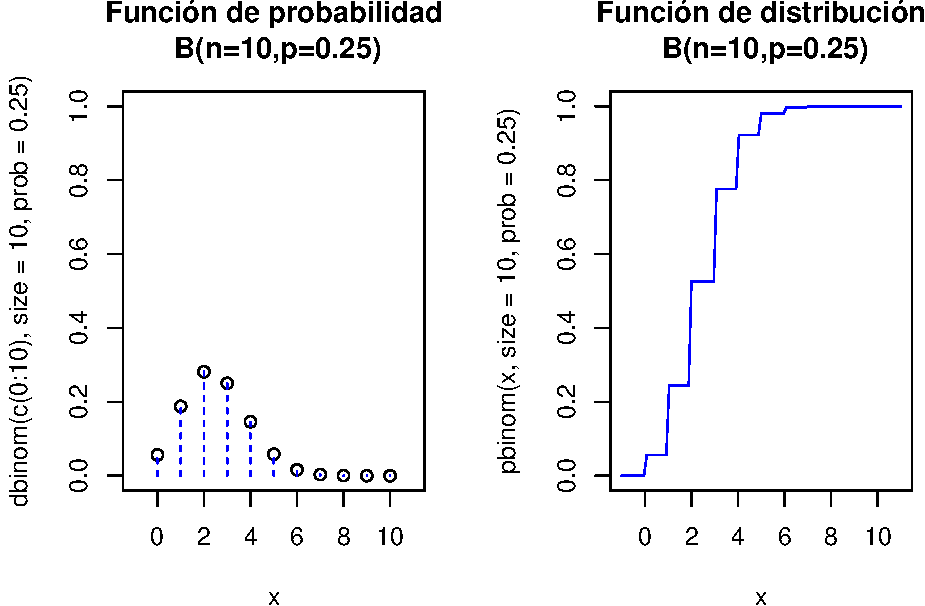
\includegraphics{curso-probabilidad-udemy_files/figure-latex/unnamed-chunk-21-1} \end{center}

\hypertarget{gruxe1ficas-interactivas-binomial}{%
\subsection{Gráficas interactivas binomial}\label{gruxe1ficas-interactivas-binomial}}

Para ejecutar el siguiente gráfico interactivo, solamente tienes que cargar el paquete \texttt{shiny} en tu ordenador y luego copiar/pegar las siguientes instrucciones. De este modo podrás observar los cambios en las distribuciones variando los parámetros.

\begin{Shaded}
\begin{Highlighting}[]
\KeywordTok{fluidPage}\NormalTok{(}
\KeywordTok{fluidRow}\NormalTok{(}
  \KeywordTok{column}\NormalTok{(}\DecValTok{6}\NormalTok{,}
         \KeywordTok{sliderInput}\NormalTok{(}\StringTok{"n_binom"}\NormalTok{, }\DataTypeTok{label =} \StringTok{"Número de repeticiones n:"}\NormalTok{,}
              \DataTypeTok{min =} \DecValTok{1}\NormalTok{, }\DataTypeTok{max =} \DecValTok{50}\NormalTok{, }\DataTypeTok{value =}\DecValTok{10}\NormalTok{ , }\DataTypeTok{step =} \DecValTok{1}\NormalTok{)),}
  \KeywordTok{column}\NormalTok{(}\DecValTok{6}\NormalTok{,}
          \KeywordTok{sliderInput}\NormalTok{(}\StringTok{"p_binom"}\NormalTok{, }\DataTypeTok{label =} \StringTok{"Probabilidad éxito p:"}\NormalTok{,}
                     \DataTypeTok{min =} \FloatTok{0.01}\NormalTok{, }\DataTypeTok{max =} \FloatTok{0.99}\NormalTok{, }\DataTypeTok{value =} \FloatTok{0.25}\NormalTok{, }\DataTypeTok{step =} \FloatTok{0.01}\NormalTok{)}
\NormalTok{         )}
\NormalTok{  )}
\NormalTok{)}

\KeywordTok{renderPlot}\NormalTok{(\{}
\NormalTok{  n=input}\OperatorTok{$}\NormalTok{n_binom}
\NormalTok{  pr=input}\OperatorTok{$}\NormalTok{p_binom}
  
  \KeywordTok{par}\NormalTok{(}\DataTypeTok{mfrow=}\KeywordTok{c}\NormalTok{(}\DecValTok{1}\NormalTok{,}\DecValTok{2}\NormalTok{))}
\NormalTok{  aux=}\KeywordTok{rep}\NormalTok{(}\DecValTok{0}\NormalTok{,(n}\OperatorTok{+}\DecValTok{1}\NormalTok{)}\OperatorTok{*}\DecValTok{2}\NormalTok{)}
\NormalTok{  aux[}\KeywordTok{seq}\NormalTok{(}\DecValTok{2}\NormalTok{,(n}\OperatorTok{+}\DecValTok{1}\NormalTok{)}\OperatorTok{*}\DecValTok{2}\NormalTok{,}\DecValTok{2}\NormalTok{)]=}\KeywordTok{dbinom}\NormalTok{(}\KeywordTok{c}\NormalTok{(}\DecValTok{0}\OperatorTok{:}\NormalTok{n),}\DataTypeTok{size=}\NormalTok{n,}\DataTypeTok{prob=}\NormalTok{pr)}
  \KeywordTok{plot}\NormalTok{(}\DataTypeTok{x=}\KeywordTok{c}\NormalTok{(}\DecValTok{0}\OperatorTok{:}\NormalTok{n),}\DataTypeTok{y=}\KeywordTok{dbinom}\NormalTok{(}\KeywordTok{c}\NormalTok{(}\DecValTok{0}\OperatorTok{:}\NormalTok{n),}\DataTypeTok{size=}\NormalTok{n,}\DataTypeTok{prob=}\NormalTok{pr),}
       \DataTypeTok{ylim=}\KeywordTok{c}\NormalTok{(}\DecValTok{0}\NormalTok{,}\DecValTok{1}\NormalTok{),}\DataTypeTok{xlim=}\KeywordTok{c}\NormalTok{(}\OperatorTok{-}\DecValTok{1}\NormalTok{,n}\OperatorTok{+}\DecValTok{1}\NormalTok{),}\DataTypeTok{xlab=}\StringTok{"x"}\NormalTok{,}
       \DataTypeTok{main=}\KeywordTok{paste0}\NormalTok{(}\KeywordTok{c}\NormalTok{(}\StringTok{"Función de probabilidad}\CharTok{\textbackslash{}n}\StringTok{ B(n="}\NormalTok{,n,}\StringTok{",p="}\NormalTok{,pr,}\StringTok{")"}\NormalTok{),}\DataTypeTok{collapse =} \StringTok{""}\NormalTok{))}
  \KeywordTok{lines}\NormalTok{(}\DataTypeTok{x=}\KeywordTok{rep}\NormalTok{(}\DecValTok{0}\OperatorTok{:}\NormalTok{n,}\DataTypeTok{each=}\DecValTok{2}\NormalTok{),}\DataTypeTok{y=}\NormalTok{aux, }\DataTypeTok{type =} \StringTok{"h"}\NormalTok{, }\DataTypeTok{lty =} \DecValTok{2}\NormalTok{,}\DataTypeTok{col=}\StringTok{"blue"}\NormalTok{)}
  \KeywordTok{curve}\NormalTok{(}\KeywordTok{pbinom}\NormalTok{(x,}\DataTypeTok{size=}\NormalTok{n,}\DataTypeTok{p=}\NormalTok{pr),}
        \DataTypeTok{xlim=}\KeywordTok{c}\NormalTok{(}\OperatorTok{-}\DecValTok{1}\NormalTok{,n}\OperatorTok{+}\DecValTok{1}\NormalTok{),}\DataTypeTok{col=}\StringTok{"blue"}\NormalTok{,}
        \DataTypeTok{main=}\KeywordTok{paste0}\NormalTok{(}\KeywordTok{c}\NormalTok{(}\StringTok{"Función de distribución\textbackslash{}n B(n="}\NormalTok{,n,}\StringTok{",p="}\NormalTok{,pr,}\StringTok{")"}\NormalTok{),}
                    \DataTypeTok{collapse =} \StringTok{""}\NormalTok{))}
        \KeywordTok{par}\NormalTok{(}\DataTypeTok{mfrow=}\KeywordTok{c}\NormalTok{(}\DecValTok{1}\NormalTok{,}\DecValTok{1}\NormalTok{))}
\NormalTok{\})}
\end{Highlighting}
\end{Shaded}

\href{https://joanby.shinyapps.io/DistribucionesNotables/}{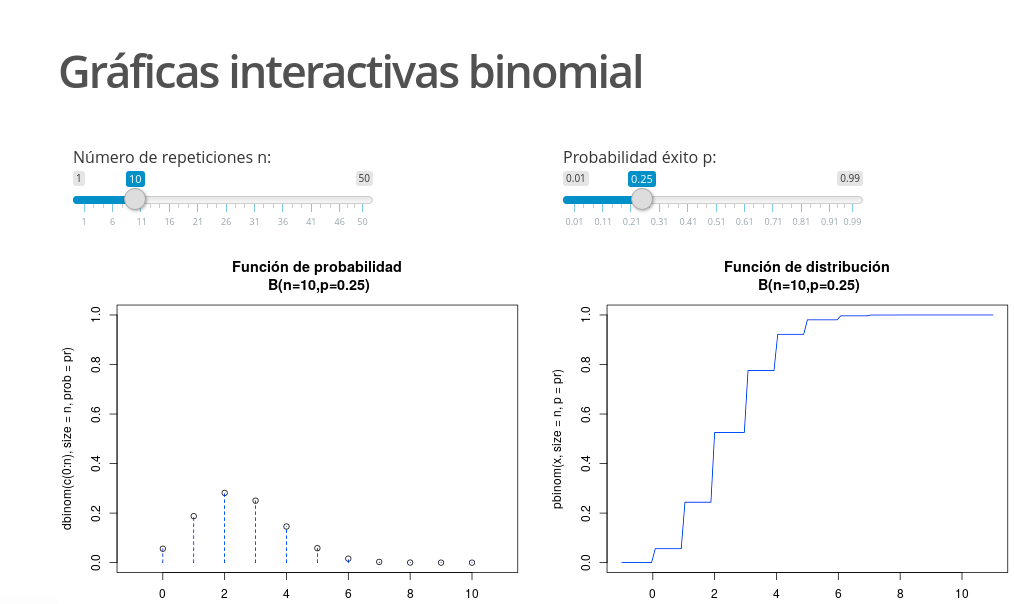
\includegraphics{Images/noshinyImages/interactiva_bino1.png}}

\hypertarget{gruxe1ficos-de-la-distribuciuxf3n-binomial-con-python}{%
\subsection{Gráficos de la distribución binomial con python}\label{gruxe1ficos-de-la-distribuciuxf3n-binomial-con-python}}

\textbf{Ejercicio}

Buscad en la documentación de python cómo se dibuja la función de probabilidad y de distribución de una binomial y recread los gráficos anteriores.

Pista: Necesitaremos investigar más librerías:

\begin{Shaded}
\begin{Highlighting}[]
\ImportTok{import}\NormalTok{ numpy }\ImportTok{as}\NormalTok{ np}
\ImportTok{import}\NormalTok{ matplotlib.pyplot }\ImportTok{as}\NormalTok{ plt}
\end{Highlighting}
\end{Shaded}

\hypertarget{gruxe1ficos-de-la-distribuciuxf3n-binomial-con-python-1}{%
\subsection{Gráficos de la distribución binomial con python}\label{gruxe1ficos-de-la-distribuciuxf3n-binomial-con-python-1}}

\begin{Shaded}
\begin{Highlighting}[]
\NormalTok{n, p }\OperatorTok{=} \DecValTok{10}\NormalTok{, }\FloatTok{0.25}
\NormalTok{x }\OperatorTok{=}\NormalTok{ np.arange(binom.ppf(}\FloatTok{0.01}\NormalTok{, n, p),binom.ppf(}\FloatTok{0.99}\NormalTok{, n, p))}
\NormalTok{fig }\OperatorTok{=}\NormalTok{plt.figure(figsize}\OperatorTok{=}\NormalTok{(}\DecValTok{5}\NormalTok{, }\FloatTok{2.7}\NormalTok{))}
\NormalTok{ax }\OperatorTok{=}\NormalTok{ fig.add_subplot(}\DecValTok{1}\NormalTok{,}\DecValTok{2}\NormalTok{,}\DecValTok{1}\NormalTok{)}
\NormalTok{ax.plot(x, binom.pmf(x, n, p), }\StringTok{'bo'}\NormalTok{, ms}\OperatorTok{=}\DecValTok{8}\NormalTok{, label}\OperatorTok{=}\StringTok{'binom pmf'}\NormalTok{)}
\NormalTok{ax.vlines(x, }\DecValTok{0}\NormalTok{, binom.pmf(x, n, p), colors}\OperatorTok{=}\StringTok{'b'}\NormalTok{, lw}\OperatorTok{=}\DecValTok{5}\NormalTok{, alpha}\OperatorTok{=}\FloatTok{0.5}\NormalTok{)}
\ControlFlowTok{for}\NormalTok{ tick }\KeywordTok{in}\NormalTok{ ax.xaxis.get_major_ticks():}
\NormalTok{  tick.label.set_fontsize(}\DecValTok{5}\NormalTok{)}
\ControlFlowTok{for}\NormalTok{ tick }\KeywordTok{in}\NormalTok{ ax.yaxis.get_major_ticks():}
\NormalTok{  tick.label.set_fontsize(}\DecValTok{5}\NormalTok{) }
\NormalTok{ax }\OperatorTok{=}\NormalTok{ fig.add_subplot(}\DecValTok{1}\NormalTok{,}\DecValTok{2}\NormalTok{,}\DecValTok{2}\NormalTok{)}
\NormalTok{ax.plot(x, binom.cdf(x, n, p), }\StringTok{'bo'}\NormalTok{, ms}\OperatorTok{=}\DecValTok{8}\NormalTok{, label}\OperatorTok{=}\StringTok{'binom pmf'}\NormalTok{)}
\NormalTok{ax.vlines(x, }\DecValTok{0}\NormalTok{, binom.cdf(x, n, p), colors}\OperatorTok{=}\StringTok{'b'}\NormalTok{, lw}\OperatorTok{=}\DecValTok{5}\NormalTok{, alpha}\OperatorTok{=}\FloatTok{0.5}\NormalTok{)}
\ControlFlowTok{for}\NormalTok{ tick }\KeywordTok{in}\NormalTok{ ax.xaxis.get_major_ticks():}
\NormalTok{  tick.label.set_fontsize(}\DecValTok{5}\NormalTok{)}
\ControlFlowTok{for}\NormalTok{ tick }\KeywordTok{in}\NormalTok{ ax.yaxis.get_major_ticks():}
\NormalTok{  tick.label.set_fontsize(}\DecValTok{5}\NormalTok{)}
\NormalTok{fig.suptitle(}\StringTok{'Distribucion Binomial'}\NormalTok{)}
\NormalTok{plt.show()}
\end{Highlighting}
\end{Shaded}

\hypertarget{gruxe1ficos-de-la-distribuciuxf3n-binomial-con-python-2}{%
\subsection{Gráficos de la distribución binomial con python}\label{gruxe1ficos-de-la-distribuciuxf3n-binomial-con-python-2}}

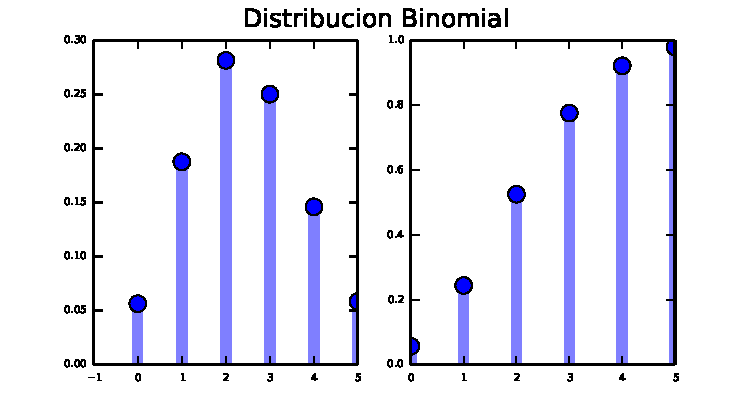
\includegraphics{curso-probabilidad-udemy_files/figure-latex/dibu_python2-1.pdf}

\hypertarget{ejemplo-distribuciuxf3n-binomial}{%
\subsection{Ejemplo distribución binomial}\label{ejemplo-distribuciuxf3n-binomial}}

\textbf{Ejemplo: Número de bolas rojas extraídas de urna con reposición.}

Tenemos una urna con \(100\) bolas de las cuales 40 son rojas y 60 blancas. Extraemos al azar una bola, anotamos su color y la devolvemos a (reponemos en ) la urna.

Supongamos que repetimos este proceso \(n=10\); reponiendo en cada ocasión la bola extraída.

Consideremos la variable aleatoria \(X=\) número de bolas rojas extraídas (con reposición) en \(n=10\) repeticiones del mismo experimento Bernoulli.

Bajo estas condiciones tenemos que repetimos \(n=10\) veces el mismo experimento Bernouilli con probabilidad de éxito (sacar bola roja) es

\[P(Roja)=P(Éxito)=p=\frac{40}{100}=0.4.\]

Así que la variable \(X=\)"número de bolas rojas extraídas de la urna (con reposición) en \(n=10\) ocasiones sigue una ley binomial \(B(n=10,p=0.4).\)

\hypertarget{ejemplo-bn10p0.4.}{%
\subsection{\texorpdfstring{Ejemplo \(B(n=10,p=0.4).\)}{Ejemplo B(n=10,p=0.4).}}\label{ejemplo-bn10p0.4.}}

Nos preguntamos:

\begin{enumerate}
\def\labelenumi{\arabic{enumi}.}
\tightlist
\item
  ¿Cuál es la probabilidad de que saquemos exactamente \(4\) rojas?
\item
  ¿Cuál es la probabilidad de que saquemos al menos \(4\) rojas?
\item
  ¿Cuál es la probabilidad de que saquemos menos de \(3\) rojas?
\item
  ¿Cuál es el valor esperado del número de bolas rojas?
\item
  ¿Cuál es la desviación típica del número de bolas rojas?
\end{enumerate}

\hypertarget{ejemplo-bn10p0.4.-1}{%
\subsection{\texorpdfstring{Ejemplo \(B(n=10,p=0.4).\)}{Ejemplo B(n=10,p=0.4).}}\label{ejemplo-bn10p0.4.-1}}

\textbf{Solución 1}. ¿Cuál es la probabilidad de que saquemos exactamente \(4\) rojas?

Utilizando al función de probabilidad tenemos que

\[
\begin{eqnarray*}
P_x(X=4)&=&{10\choose 4}\cdot 0.4^4\cdot (1-0.4)^{10-4}
= \frac{10!}{(10-4)!\cdot 4!}\cdot 0.4^4\cdot 0.6^6\\
&=& \frac{7\cdot 8\cdot 9\cdot 10}{1\cdot 2\cdot 3\cdot 4}\cdot 0.4^4\cdot 0.6^6=0.2508227
\end{eqnarray*}
.
\]

Con R

\begin{Shaded}
\begin{Highlighting}[]
\KeywordTok{dbinom}\NormalTok{(}\DecValTok{4}\NormalTok{,}\DataTypeTok{size=}\DecValTok{10}\NormalTok{,}\DataTypeTok{prob =} \FloatTok{0.4}\NormalTok{)}
\end{Highlighting}
\end{Shaded}

\begin{verbatim}
## [1] 0.2508227
\end{verbatim}

\hypertarget{ejemplo-bn10p0.4.-2}{%
\subsection{\texorpdfstring{Ejemplo \(B(n=10,p=0.4).\)}{Ejemplo B(n=10,p=0.4).}}\label{ejemplo-bn10p0.4.-2}}

\textbf{Solución 2}. ¿Cuál es la probabilidad de que saquemos al menos \(4\) rojas?

Al menos 4 rojas es \(P(X \geq 4)=1-P(X<4)=1-P(x\leq 3).\)

Así que calculemos \(P(X\leq 3)\)

\[
\begin{eqnarray*}
P(x\leq 3)&=& P(X=0)+P(X=1)+P(X=2)+P(X=3)\\
&=& 
 {10\choose 0}\cdot 0.4^0\cdot (1-0.4)^{10-0}+ {10\choose 1}\cdot 0.4^1\cdot (1-0.4)^{10-1}\\
&+&{10\choose 2}\cdot 0.4^2\cdot (1-0.4)^{10-2}+ {10\choose 3}\cdot 0.4^3\cdot (1-0.4)^{10-3}\\
&=&0.3822806
\end{eqnarray*}
.
\]

\hypertarget{ejemplo-bn10p0.4.-3}{%
\subsection{\texorpdfstring{Ejemplo \(B(n=10,p=0.4).\)}{Ejemplo B(n=10,p=0.4).}}\label{ejemplo-bn10p0.4.-3}}

Con R

\begin{Shaded}
\begin{Highlighting}[]
\KeywordTok{pbinom}\NormalTok{(}\DecValTok{3}\NormalTok{,}\DecValTok{10}\NormalTok{,}\FloatTok{0.4}\NormalTok{)}
\end{Highlighting}
\end{Shaded}

\begin{verbatim}
## [1] 0.3822806
\end{verbatim}

Así que

\[P(X \geq 4 )=1-P(x< 4)=P(X\leq 3)=1-0.3822806=0.6177194.\]

\hypertarget{ejemplo-bn10p0.4.-4}{%
\subsection{\texorpdfstring{Ejemplo \(B(n=10,p=0.4).\)}{Ejemplo B(n=10,p=0.4).}}\label{ejemplo-bn10p0.4.-4}}

O con R también

\begin{Shaded}
\begin{Highlighting}[]
\DecValTok{1}\OperatorTok{-}\KeywordTok{pbinom}\NormalTok{(}\DecValTok{3}\NormalTok{,}\DecValTok{10}\NormalTok{,}\FloatTok{0.4}\NormalTok{)}
\end{Highlighting}
\end{Shaded}

\begin{verbatim}
## [1] 0.6177194
\end{verbatim}

Aunque en estos casos el parámetro \texttt{lower.tail\ =\ FALSE} es sin duda nuestra mejor opción:

\begin{Shaded}
\begin{Highlighting}[]
\KeywordTok{pbinom}\NormalTok{(}\DecValTok{3}\NormalTok{,}\DecValTok{10}\NormalTok{,}\FloatTok{0.4}\NormalTok{,}\DataTypeTok{lower.tail =} \OtherTok{FALSE}\NormalTok{)}
\end{Highlighting}
\end{Shaded}

\begin{verbatim}
## [1] 0.6177194
\end{verbatim}

\hypertarget{ejemplo-bn10p0.4.-5}{%
\subsection{\texorpdfstring{Ejemplo \(B(n=10,p=0.4).\)}{Ejemplo B(n=10,p=0.4).}}\label{ejemplo-bn10p0.4.-5}}

\textbf{Solución 3}. ¿Cuál es la probabilidad de que saquemos menos de \(3\) rojas?

\[
\begin{eqnarray*}
P(x< 3)&=& P(X\leq 2)=  P(X=0)+P(X=1)+P(X=2)\\
&=& 
{10\choose 0}\cdot 0.4^0\cdot (1-0.4)^{10-0}+ {10\choose 1}\cdot 0.4^1\cdot (1-0.4)^{10-1}\\
&+&
{10\choose 2}\cdot 0.4^2\cdot (1-0.4)^{10-2}\\
&=&0.1672898
\end{eqnarray*}
.
\]

\begin{Shaded}
\begin{Highlighting}[]
\KeywordTok{dbinom}\NormalTok{(}\DecValTok{0}\NormalTok{,}\DecValTok{10}\NormalTok{,}\FloatTok{0.4}\NormalTok{)}\OperatorTok{+}\KeywordTok{dbinom}\NormalTok{(}\DecValTok{1}\NormalTok{,}\DecValTok{10}\NormalTok{,}\FloatTok{0.4}\NormalTok{)}\OperatorTok{+}\KeywordTok{dbinom}\NormalTok{(}\DecValTok{2}\NormalTok{,}\DecValTok{10}\NormalTok{,}\FloatTok{0.4}\NormalTok{)}
\end{Highlighting}
\end{Shaded}

\begin{verbatim}
## [1] 0.1672898
\end{verbatim}

\begin{Shaded}
\begin{Highlighting}[]
\KeywordTok{pbinom}\NormalTok{(}\DecValTok{2}\NormalTok{,}\DecValTok{10}\NormalTok{,}\FloatTok{0.4}\NormalTok{)}
\end{Highlighting}
\end{Shaded}

\begin{verbatim}
## [1] 0.1672898
\end{verbatim}

\hypertarget{ejemplo-bn10p0.4.-6}{%
\subsection{\texorpdfstring{Ejemplo \(B(n=10,p=0.4).\)}{Ejemplo B(n=10,p=0.4).}}\label{ejemplo-bn10p0.4.-6}}

\textbf{Solución 4}. ¿Cuál es el valor esperado del número de bolas rojas?

Como \(X\) es una \(B(n=10,p=0.4)\) sabemos que

\[E(X)=n\cdot p = 10\cdot 0.4=4.\]

Aunque en python tenemos la función stats que nos lo calcula directamente:

\begin{Shaded}
\begin{Highlighting}[]
\BuiltInTok{print}\NormalTok{(}\StringTok{"E(X) = }\SpecialCharTok{\{m\}}\StringTok{"}\NormalTok{.}\BuiltInTok{format}\NormalTok{(m}\OperatorTok{=}\NormalTok{binom.stats(n }\OperatorTok{=} \DecValTok{10}\NormalTok{, p }\OperatorTok{=} \FloatTok{0.4}\NormalTok{, moments}\OperatorTok{=}\StringTok{'m'}\NormalTok{)))}
\end{Highlighting}
\end{Shaded}

\begin{verbatim}
## E(X) = 4.0
\end{verbatim}

\hypertarget{ejemplo-bn10p0.4.-7}{%
\subsection{\texorpdfstring{Ejemplo \(B(n=10,p=0.4).\)}{Ejemplo B(n=10,p=0.4).}}\label{ejemplo-bn10p0.4.-7}}

\textbf{Solución 5}. ¿Cuál es la desviación típica del número de bolas rojas?

La varianza es

\[
Var(X)=n\cdot p \cdot(1-p)=10\cdot 0.4\cdot 0.6=2.4.
\]

Por lo tanto la desviación típica es

\[\sqrt{Var(X)}=\sqrt{2.4}= 1.5491933.\]

Aunque en python tenemos la función stats que nos lo calcula directamente:

\begin{Shaded}
\begin{Highlighting}[]
\BuiltInTok{print}\NormalTok{(}\StringTok{"Var(X) = }\SpecialCharTok{\{v\}}\StringTok{"}\NormalTok{.}\BuiltInTok{format}\NormalTok{(v}\OperatorTok{=}\NormalTok{binom.stats(n }\OperatorTok{=} \DecValTok{10}\NormalTok{, p }\OperatorTok{=} \FloatTok{0.4}\NormalTok{, moments}\OperatorTok{=}\StringTok{'v'}\NormalTok{)))}
\end{Highlighting}
\end{Shaded}

\begin{verbatim}
## Var(X) = 2.4
\end{verbatim}

\hypertarget{distribuciuxf3n-geomuxe9trica}{%
\section{Distribución geométrica}\label{distribuciuxf3n-geomuxe9trica}}

\hypertarget{distribuciuxf3n-geomuxe9trica-1}{%
\subsection{Distribución geométrica}\label{distribuciuxf3n-geomuxe9trica-1}}

\begin{itemize}
\item
  Todos hemos jugado a, por ejemplo, tirar una moneda hasta que obtengamos la primera cara.
\item
  O también tirar una pelota a una canasta de baloncesto hasta obtener la primer la canasta.
\item
  Desde otro punto de vista también podemos intentar modelar el número de veces que accionamos una interruptor y la bombilla se ilumina hasta que falla.
\item
  O también el número de veces que un cajero automático nos da dinero hasta que falla.
\end{itemize}

La \textbf{modelización de este tipo de problemas se consigue con la llamada distribución geométrica}.

\hypertarget{distribuciuxf3n-geomuxe9trica-2}{%
\subsection{Distribución geométrica}\label{distribuciuxf3n-geomuxe9trica-2}}

 Distribución geométrica

\begin{itemize}
\tightlist
\item
  Repitamos un experimento Bernoulli, de parámetro p, de forma independiente hasta obtener el primer éxito.
\item
  Sea \(X\) la v.a. que cuenta el número de fracasos antes del primer éxito. Por ejemplo que hayamos tenido \(x\) fracasos será una cadena de \(x\) fracasos culminada con un éxito. Más concretamente
\end{itemize}

\[P(\overbrace{FFF\ldots F}^{x}E)=P(F)^{x}\cdot P(E)=(1-p)^{x}\cdot p=q^{x}\cdot p.\]

\hypertarget{distribuciuxf3n-geomuxe9trica-3}{%
\subsection{Distribución geométrica}\label{distribuciuxf3n-geomuxe9trica-3}}

Su función de probabilidad es

\[
P_X(x)=P(X=x)=\left\{\begin{array}{ll}
(1-p)^{x}\cdot p & \mbox{ si } x=0,1,2,\ldots\\
0 &\mbox{ en otro caso}
\end{array}\right..
\]

\begin{itemize}
\tightlist
\item
  De una v.a. como esta diremos que sigue una
  distribución geométrica de parámetro \(p\).
\item
  La denotaremos por \(Ge(p)\).
\item
  Su dominio es \(D_X=\{0,1,2,\ldots\}\).
\end{itemize}

\hypertarget{funciuxf3n-de-distribuciuxf3n-geomuxe9trica}{%
\subsection{Función de distribución geométrica}\label{funciuxf3n-de-distribuciuxf3n-geomuxe9trica}}

Calculemos P(\(X\leq 3\)).

Por la propiedad de la probabilidad del suceso complementario tenemos que

\[
P(X\leq 3 )=1-P(X> 3)=1-P(X\geq 4)
\]

Efectivamente, el evento tenemos que \(X\leq 3\) es que hemos fracasado más de tres veces hasta conseguir el primer éxito; es decir \textbf{hemos fracasado 4 o más veces}, por lo tanto

\[
\{X>3\}=\{X\geq 4\}= \{FFFF\}
\]

\hypertarget{funciuxf3n-de-distribuciuxf3n-geomuxe9trica-1}{%
\subsection{Función de distribución geométrica}\label{funciuxf3n-de-distribuciuxf3n-geomuxe9trica-1}}

Ahora, al ser los intentos sucesos independientes, tenemos que:

\[
\begin{eqnarray*}
P(X>3) & = & P(\{FFFF\})= P(F)\cdot P(F)\cdot P(F)\cdot P(F)\\
&=& (1-p)\cdot (1-p)\cdot (1-p)\cdot (1-p)= (1-p)^{3+1}\\\
&=&(1-p)^{4}.
\end{eqnarray*}
\]

Calculamos

\[F_X(3)=P(X\leq 3)=1-P(X>3)=1-(1-p)^{3+1}.\]

Por lo que podemos generalizar a cualquier entero positivo \(k=0,1,2,\ldots\)

\[F_X(k)=P(X\leq k)=1-(1-p)^{k+1}\mbox{ si } k=0,1,2,\ldots\]

\hypertarget{funciuxf3n-de-distribuciuxf3n-geomuxe9trica-2}{%
\subsection{Función de distribución geométrica}\label{funciuxf3n-de-distribuciuxf3n-geomuxe9trica-2}}

En general tendremos que

\[
F_X(x)=P(X\leq x)=
\left\{\begin{array}{ll} 
0 & \mbox{ si } x<0\\
1- (1-p)  & \mbox{ si } k=0\leq x <1\\
1- (1-p)^2 & \mbox{ si } k=1\leq x <2\\
1- (1-p)^3 & \mbox{ si } k=2\leq x <3\\
1- (1-p)^{k+1} & \mbox{ si } \left\{ \begin{array}{l}k\leq x< k+1\\\mbox{para } k=0,1,2,\ldots\end{array}
    \right.\end{array}\right.
\]

\hypertarget{funciuxf3n-de-distribuciuxf3n-geomuxe9trica-3}{%
\subsection{Función de distribución geométrica}\label{funciuxf3n-de-distribuciuxf3n-geomuxe9trica-3}}

De forma más compacta tendremos que

\[
F_X(x)=P(X\leq x)=
\left\{\begin{array}{ll} 
0 & \mbox{ si } x<0\\
1- (1-p)^{k+1} & \mbox{ si } \left\{ \begin{array}{l}k\leq x< k+1\\\mbox{para } k=0,1,2,\ldots\end{array}
    \right.\end{array}
    \right.
\]

Notemos que si \(k=0,1,2,\ldots\) el límite de la función de distribución es

\[
\displaystyle\lim_{k\to +\infty } F_X(k)=\lim_{k\to +\infty } 1-(1-p)^{k+1}=
1
\]

ya que \(0<1-p<1\).

\hypertarget{sumas-derivadas-series-geomuxe9tricas}{%
\subsection{Sumas derivadas series geométricas}\label{sumas-derivadas-series-geomuxe9tricas}}

Recordemos del tema de variables aleatorias que

Propiedades

\begin{itemize}
\tightlist
\item
  Si \(|r|<1\) también son convergentes las derivadas, respecto de \(r\), de la serie geométrica y convergen a la derivada correspondiente. Así tenemos que
  \[
  \begin{eqnarray*}
  \left(\sum_{k=0}^{+\infty} r^k\right)'&= & \sum_{k=1}^{+\infty}k\cdot
  r^{k-1} &=& \left(\frac1{1-r}\right)'=\frac1{(1-r)^2}\\
  \left(\sum_{k=0}^{+\infty} r^k\right)^{''}&=& \sum_{k=2}^{+\infty}k \cdot(k-1)\cdot
  r^{k-2}&=&\left(\frac1{1-r}\right)^{''}=\frac2{(1-r)^3}
  \end{eqnarray*}.
  \]
\end{itemize}

\hypertarget{esperanza-de-una-v.a.-gep}{%
\subsection{\texorpdfstring{Esperanza de una v.a. \(Ge(p)\)}{Esperanza de una v.a. Ge(p)}}\label{esperanza-de-una-v.a.-gep}}

Recordemos que \(P(X=x)=(1-p)^x\cdot p\) si \(x=0,1,2,\ldots\) y aplicado la fórmula anterior con \(r=1-p\)

\[
\begin{eqnarray*}
E(X)&=&\sum_{x=0}^{+\infty} x\cdot P_x(x)=\sum_{x=0}^{+\infty} x\cdot (1-p)^x\cdot p=
p\cdot (1-p) \cdot \sum_{x=1}^{+\infty} x\cdot (1-p)^{x-1}\\
&=& p\cdot (1-p)\cdot \frac{1}{(1-(1-p))^2}=p\cdot (1-p)\cdot \frac{1}{p^2}=\frac{1-p}{p}
\end{eqnarray*}.
\]

\hypertarget{valor-ex2-de-una-v.a.-gep}{%
\subsection{\texorpdfstring{Valor \(E(X^2)\) de una v.a. \(Ge(p)\)}{Valor E(X\^{}2) de una v.a. Ge(p)}}\label{valor-ex2-de-una-v.a.-gep}}

\[
\begin{eqnarray*}
E(X^2)&=&\sum_{x=0}^{+\infty} x^2\cdot P_X(x)=\sum_{x=1}^{+\infty} x^2\cdot (1-p)^x\cdot p\\
&=& 
\sum_{x=1}^{+\infty} (x\cdot (x-1)+x)\cdot (1-p)^{x}\cdot p\\
&=&
\sum_{x=1}^{+\infty} x\cdot (x-1)\cdot (1-p)^{x}\cdot p+\sum_{x=1}^{+\infty} x \cdot (1-p)^{x}\cdot p\\
&=&
(1-p)^{2}\cdot p\cdot \sum_{x=2}^{+\infty} x\cdot (x-1)\cdot (1-p)^{x-2}\\ 
&  +&   (1-p)\cdot p\sum_{x=1}^{+\infty} x \cdot (1-p)^{x-1} = \ldots
\end{eqnarray*}.
\]

\hypertarget{valor-ex2-de-una-v.a.-gep-1}{%
\subsection{\texorpdfstring{Valor \(E(X^2)\) de una v.a. \(Ge(p)\)}{Valor E(X\^{}2) de una v.a. Ge(p)}}\label{valor-ex2-de-una-v.a.-gep-1}}

\[
\begin{eqnarray*}
E(X^2)&=&\ldots\\
&=&
(1-p)^{2}\cdot p\cdot \sum_{x=2}^{+\infty} x\cdot (x-1)\cdot (1-p)^{x-2}\\ 
&  +&   (1-p)\cdot p\sum_{x=1}^{+\infty} x \cdot (1-p)^{x-1}\\
&=&
p\cdot (1-p)^2 \frac{2}{(1-(1-p))^3}+  (1-p)\cdot p \frac{1}{(1-(1-p))^2}\\
&=&
p\cdot (1-p)^2 \frac{2}{p^3}+  (1-p)\cdot p \frac{1}{p^2}\\
&=&\frac{2\cdot (1-p)^2}{p^2}+\frac{1-p}{p}
\end{eqnarray*}.
\]

\hypertarget{varianza-de-una-v.a.-gep}{%
\subsection{\texorpdfstring{Varianza de una v.a. \(Ge(p)\)}{Varianza de una v.a. Ge(p)}}\label{varianza-de-una-v.a.-gep}}

\[
\begin{eqnarray*}
Var(X)&=&E(X^2)-E(X)^2=\frac{2\cdot (1-p)^2}{p^2}+\frac{1-p}{p}-\left(\frac{1-p}{p}\right)^2\\
&=&
\frac{2\cdot (1-p)^2+p\cdot(1-p)-(1-p)^2}{p^2}=\frac{(1-p)^2+p\cdot(1-p)}{p^2}\\
&=&
\frac{1-2\cdot p + p^2+p-p^2}{p^2}\\
&=& \frac{1-p}{p^2}.
\end{eqnarray*}
\]
Y su desviación típica será

\[\sqrt{Var(X)}=\sqrt{\frac{1-p}{p^2}}.\]

\hypertarget{resumen-gep-empezando-en-0}{%
\subsection{\texorpdfstring{Resumen \(Ge(p)\) empezando en 0}{Resumen Ge(p) empezando en 0}}\label{resumen-gep-empezando-en-0}}

\begin{longtable}[]{@{}rl@{}}
\toprule
\begin{minipage}[b]{0.51\columnwidth}\raggedleft
\(X=\) Geométrica (empieza en \(0\))\strut
\end{minipage} & \begin{minipage}[b]{0.43\columnwidth}\raggedright
número de fracasos para conseguir el primer éxito\strut
\end{minipage}\tabularnewline
\midrule
\endhead
\begin{minipage}[t]{0.51\columnwidth}\raggedleft
\(D_X=\)\strut
\end{minipage} & \begin{minipage}[t]{0.43\columnwidth}\raggedright
\(\{0,1,\ldots n,\ldots\}\)\strut
\end{minipage}\tabularnewline
\begin{minipage}[t]{0.51\columnwidth}\raggedleft
\(P_X(x)=P(X=x)=\)\strut
\end{minipage} & \begin{minipage}[t]{0.43\columnwidth}\raggedright
\(\left\{\begin{array}{ll}(1-p)^{x}\cdot p & \mbox{ si } x=0,1,2,\ldots \\0 & \mbox{ en otro caso.}\end{array}\right.\)\strut
\end{minipage}\tabularnewline
\begin{minipage}[t]{0.51\columnwidth}\raggedleft
\(F_X(x)=P(X\leq X)=\)\strut
\end{minipage} & \begin{minipage}[t]{0.43\columnwidth}\raggedright
\(\left\{\begin{array}{ll} 0 & \mbox{ si } x<0\\  1- (1-p)^{k+1} & \mbox{ si } \left\{ \begin{array}{l}k\leq x< k+1\\\mbox{para } k=0,1,2,\ldots\end{array}  \right.\end{array}\right.\)\strut
\end{minipage}\tabularnewline
\begin{minipage}[t]{0.51\columnwidth}\raggedleft
\(E(X)=\frac{1-p}{p}\)\strut
\end{minipage} & \begin{minipage}[t]{0.43\columnwidth}\raggedright
\(Var(X)=\frac{1-p}{p^2}\)\strut
\end{minipage}\tabularnewline
\bottomrule
\end{longtable}

\hypertarget{la-variable-geomuxe9trica-que-cuenta-los-intentos-para-obtener-el-primer-uxe9xito.}{%
\subsection{La variable geométrica que cuenta los intentos para obtener el primer éxito.}\label{la-variable-geomuxe9trica-que-cuenta-los-intentos-para-obtener-el-primer-uxe9xito.}}

\begin{itemize}
\tightlist
\item
  Supongamos que sólo estamos interesados en el \textbf{número de intentos} para obtener el primer éxito.
\item
  Si definimos \(Y\)= número de intentos para obtener el primer éxito. Entonces \(Y=X+1\) donde \(X\equiv Ge(p)\).
\item
  Su dominio es valores es \(D_Y=\{1,2,\ldots\}\)
\item
  la media se incrementa en un intento debido al éxito \(E(Y)=E(X+1)=E(X)+1=\frac{1-p}{p}+1=\frac1{p}\).
\item
  La varianza es la misma \(Var(Y)=Var(X+1)=Var(X)=\frac{1-p}{p^2}\).
\end{itemize}

\hypertarget{resumen-gep-comenzando-en-1.}{%
\subsection{\texorpdfstring{Resumen \(Ge(p)\) comenzando en \(1\).}{Resumen Ge(p) comenzando en 1.}}\label{resumen-gep-comenzando-en-1.}}

\begin{longtable}[]{@{}rl@{}}
\toprule
\begin{minipage}[b]{0.51\columnwidth}\raggedleft
\(Y\) geométrica (que cuenta el éxito empieza en 1)\strut
\end{minipage} & \begin{minipage}[b]{0.43\columnwidth}\raggedright
número de INTENTOS para OBTENER el primer éxito\strut
\end{minipage}\tabularnewline
\midrule
\endhead
\begin{minipage}[t]{0.51\columnwidth}\raggedleft
\(D_Y=\)\strut
\end{minipage} & \begin{minipage}[t]{0.43\columnwidth}\raggedright
\(\{1,2,\ldots n,\ldots\}\)\strut
\end{minipage}\tabularnewline
\begin{minipage}[t]{0.51\columnwidth}\raggedleft
\(P_Y(y)=P(Y=y)=\)\strut
\end{minipage} & \begin{minipage}[t]{0.43\columnwidth}\raggedright
\(\left\{\begin{array}{ll}(1-p)^{y-1}\cdot p & \mbox{ si } y=1,2,3,\ldots\\ 0 & \mbox{ en otro caso.}\end{array}\right.\)\strut
\end{minipage}\tabularnewline
\begin{minipage}[t]{0.51\columnwidth}\raggedleft
\(F_Y(y)=P(Y\leq y)=\)\strut
\end{minipage} & \begin{minipage}[t]{0.43\columnwidth}\raggedright
\(\left\{\begin{array}{ll} 0 & \mbox{ si } y<1\\ 1- (1-p)^{k} & \mbox{ si } \left\{ \begin{array}{l}k\leq y< k+1\\\mbox{para } k=1,2,3,\dots \end{array} \right.\end{array}\right.\)\strut
\end{minipage}\tabularnewline
\begin{minipage}[t]{0.51\columnwidth}\raggedleft
\(E(X)=\frac1{p}\)\strut
\end{minipage} & \begin{minipage}[t]{0.43\columnwidth}\raggedright
\(Var(X)=\frac{1-p}{p^2}\)\strut
\end{minipage}\tabularnewline
\bottomrule
\end{longtable}

\hypertarget{propiedad-de-la-falta-de-memoria}{%
\subsection{Propiedad de la falta de memoria}\label{propiedad-de-la-falta-de-memoria}}

 Propiedad de la falta de memoria

Sea \(X\) una v.a. discreta con dominio \(D_X=\{0,1,2,\ldots\}\), con \(P(X=0)=p\).

Entonces \(X\) sigue una ley \(Ge(p)\) sí y sólo si

\[
P\left(X> k+j\big| X\geq j\right)=P(X> k)
\]
para todo \(k,j=0,1,2,3\ldots\).

\hypertarget{propiedad-de-la-falta-de-memoria-1}{%
\subsection{Propiedad de la falta de memoria}\label{propiedad-de-la-falta-de-memoria-1}}

\textbf{Demostración}

Si es geométrica entonces el lado derecho de la igualdad es

\[
P(X>k)=1-P(X\leq k)=1-\left(1-(1-p)^{k+1}\right)=(1-p)^{k+1}
\]

El lado de izquierdo es

\[
\begin{eqnarray*} 
P\left(X> k+j\big| X\geq j\right)&=&\frac{P\left(\{X> k+j\}\cap \{X\geq j\} \right)}{P\left(X\geq j\right)}=
\frac{P\left(X>k+j \right)}{P\left(X\geq j \right)} = \frac{1-P(X\leq k+j)}{1-P(X\leq j-1)}\\
&=&  \frac{1-(1-(1-p)^{k+j+1})}{1-(1-(1-p)^{j-1+1})} =\frac{(1-p)^{k+j+1}}{(1-p)^{j}} = (1-p)^{k+1}
\end{eqnarray*}
\]

Lo que demuestra la igualdad.

Para demostrar el recíproco tomemos \(j=1\) y \(k\geq 0\) entonces por la propiedad de la pérdida de memoria

\[
P\left(X> k+1\big| X\geq 1\right)=P(X> k)
\]

Como sabemos \(P(X=0)=p\) tenemos \(P(X \geq 1 )=1-P(X<1)=1-P(X=0)=1-p\)

Luego combinado las igualdades tenemos que

\[
P\left(X> k+1\big| X\geq 1\right)=\frac{P(X>k+1, X\geq 1)}{P(X\geq 1)}=\frac{P(X>k+1)}{P(X\geq 1)}=P(X>k).
\]
Así podemos poner que

\[
\begin{eqnarray*}
P(X>k+1)&=&P(X\geq 1)\cdot P(X>k)=\left(1-P(X<1)\right)\cdot P(X>k)\\
&=&\left(1-P(X=0)\right)\cdot P(X>k)=(1-p)\cdot P(X>k).
\end{eqnarray*}
\]

Es decir en general tenemos que

\[
P(X>k+1)=(1-p)\cdot P(X>k)
\]
Del mismo modo para \(j=2\)

\[
P(X>k+2)=(1-p)\cdot P(X>k+1)
\]

Restando la primera igualdad de la última obtenemos.

\[
P(X>k+1)-P(X>k+2)=(1-p)\cdot P(X>k)-(1-p)\cdot P(X>k+1)
\]

de donde operando en cada lado de la igualdad obtenemos la recurrencia

\[
[1-P(X\leq k+1)]-[1-P(X\leq k+2)]=(1-p)\cdot [P(X>k)-P(X>k+1)]
\]

Ahora operando

\[
P(X\leq k+2)-P(X\leq k+1)=(1-p)\cdot[1-P(X\leq k)-\left(1-P(X\leq k+1)\right)]
\]
\[
P(X=k+2)=(1-p)\cdot[P(X\leq k+1)-P(X\leq k)]
\]
\[
P(X=k+2)=(1-p)\cdot P(X=k+1)
\]

De forma similar obtenemos

\[
P(X=k+1)=(1-p)\cdot P(X=k)
\]
Utilicemos la recurrencia anterior para calcular todas las probabilidades a partir de la \(P(X=0)=p\); que vienen dadas por:

\[
\begin{eqnarray*}
P(X=0)&=& p\\
P(X=1)&=&P(X=0+1)= (1-p)\cdot P(X=0) =(1-p)\cdot  p\\
P(X=2)&=&P(X=1+1)= (1-p)\cdot P(X=1)=(1-p)\cdot (1-p)\cdot p=(1-p)^2\cdot p\\
\ldots \ldots\ldots && \ldots  \ldots \ldots \ldots\ldots\ldots\ldots\ldots\ldots\ldots\ldots\ldots\ldots\ldots\ldots\ldots\ldots\ldots\ldots\ldots\ldots\ldots\ldots\ldots\\
P(X=k)&=&P(X=(k-1)+1)= (1-p)\cdot P(X=k-1)=(1-p)\cdot (1-p)^{k-1}\cdot p=(1-p)^{k}\cdot p
\end{eqnarray*}.
\]
Lo que demuestra el recíproco, es decir que \(X\) es \(Geom(p)\).

\hypertarget{falta-de-memoria}{%
\subsection{Falta de memoria}\label{falta-de-memoria}}

 Observación: Interpretación de la propiedad

La propiedad de la falta de memoria

\[
P(X> k+j\big|X \geq j)=P(X > k)
\]

la igualdad anterior significa que aunque \textbf{ya llevemos al menos \(j\) fracasos} la probabilidad de \textbf{que fracasemos \(k\) veces más} no disminuye; es la misma que si empezáramos de nuevo el experimento.

A este efecto se le suele etiquetar con la frase \textbf{el experimento carece de memoria} o es un \textbf{experimento sin memoria} (\emph{Memoryless Property}).

\hypertarget{ejemplo-falta-de-memoria}{%
\subsection{Ejemplo falta de memoria}\label{ejemplo-falta-de-memoria}}

Un ejemplo muy sencillo nos aclarará el alcance de esta propiedad

\textbf{Ejercicio: la llave que abre la puerta}

Tenemos un llavero con 10 llaves, solo una de ellas abre una puerta. Cada vez que probamos una llave y falla olvidamos que llave hemos probado. ¿Cuál es la probabilidad de que si ya lo hemos intentado 5 veces necesitemos más de 4 intentos adicionales para abrir la puerta?

Tomemos \(k=4,j=5\), aplicando la propiedad de la falta de memoria

\[
P(X> 4+5/X \geq 5)=P(X > 4)
\]

Después de 5 fracasos no estamos \emph{más cerca} de abrir la puerta.
La propiedad de la falta de memoria nos dice que en \textbf{después de cada intento es como si empezásemos de nuevo a abrir la puerta}. Tras 5 fracasos la probabilidad de que fallemos más de 4 veces más es la misma.

\hypertarget{ejemplo-falta-de-memoria-1}{%
\subsection{Ejemplo falta de memoria}\label{ejemplo-falta-de-memoria-1}}

¿Cuál es el número esperado de fracasos hasta abrir la puerta

\[
E(X)=\frac{1-p}{p}=\frac{1-\frac{1}{10}}{\frac{1}{10}}=\frac{\frac{9}{10}}{\frac{1}{10}}=9.
\]

La varianza es

\[
Var(X)=\frac{1-p}{p^2}=\frac{1-\frac{1}{10}}{\left(\frac{1}{10}\right)^2}=\frac{\frac{9}{10}}{\frac{1}{100}}=
90.
\]

La desviación típica es \(\sqrt{90}=9.486833.\)

\hypertarget{ejemplo-el-cluxe1sico-del-fuxfatbol}{%
\subsection{Ejemplo: El clásico del fútbol}\label{ejemplo-el-cluxe1sico-del-fuxfatbol}}

\textbf{Ejemplo: partidos hasta que el Barça gana al Madrid}

Los partidos Real Madrid FC Barcelona de \textbf{la liga} española se suelen denominar \textbf{El Clásico}, sean en el Bernabeu (estadio del Real Madrid) o en el Camp Nou (estadio del Barça)

Sea \(Y\) la variable que cuenta el número de veces que en un partido de fútbol de la liga el Real Madrid pierde contra el Barça sea en el Camp Nou o el Calderón.

Nuestra amiga Aina es muy culé (hincha del Barça) quiere averiguar cuántos partidos consecutivos de \textbf{El Clásico} tiene que ver hasta ver ganar al Barça por primera vez.

Le interesa estimar cuánto le va a costar este capricho. Tendrá que comprar las entradas y pagar los viajes de Barcelona a Madrid.

Para ello consulta \href{https://es.wikipedia.org/wiki/El_Cl\%C3\%A1sico}{datos historicos de \textbf{El clásico} en la wikipedia} y averigua que hasta el 3 de marzo de 2019 el Real Madrid ganó en 72 ocasiones el Barça en 72 y empataron 34 veces, en total se han jugado 178 \textbf{Clásicos}.

La pregunta es: ¿Cuál es la probabilidad de no ver ganar al Barça en al menos tres partidos consecutivos?

\hypertarget{variable-geomuxe9trica-el-cluxe1sico}{%
\subsection{Variable geométrica: El clásico}\label{variable-geomuxe9trica-el-cluxe1sico}}

Como nuestro aficionada tiene un tía que juega mucho al fútbol en su consola y con los datos que le damos estima que la probabilidad de que el Barça gane un clásico cualquiera es

\[P(Barça)=\frac{72}{178}=0.4045.\]

Supongamos pues que nuestro \emph{experimento de fútbol} sigue una ley geométrica con probabilidad de éxito \(p=P(Barça)=\frac{72}{178}.\)

Entonces si \(X\) es el número de partidos que pierde el Barça antes de que gane el primero seguirá una ley \(Ge(p=\frac{72}{178})\).

Así que lo que nos pregunta Aina es la siguiente probabilidad

\[P(X>3)=1-P(X\leq 3)=1-\left(1-\frac{72}{178}\right)^4=0.8742.\]

Así que Aina tiene una probabilidad del \(87.42\%\) de que necesite ver al menos no ganar al Barça 3 partidos antes de ver uno en el que gane.

\hypertarget{variable-geomuxe9trica-el-cluxe1sico-1}{%
\subsection{Variable geométrica: El clásico}\label{variable-geomuxe9trica-el-cluxe1sico-1}}

\textbf{Ejercicio}

Bajo las condiciones del problema Barça-Madrid de nuestra amiga Aina ¿cuál es el valor esperado de \(X\)? ¿y su varianza?

\[X=Ge\left(p=\frac{72}{178}=0.4045\right)\]

entonces

\[E(X)=\frac{1-p}{p}=\frac{1-0.4045}{0.4045}=1.4722\]

y

\[Var(X)=\frac{1-p}{p^2}=\frac{1-0.4045}{0.4045^2}=3.6397\]

La desviación típica es
\[\sqrt{3.6397}=1.9078.\]

\hypertarget{cuxe1lculos-con-r}{%
\subsection{Cálculos con R}\label{cuxe1lculos-con-r}}

Veamos los cálculos básicos con R para la distribución geométrica \(Ge(p=0.25)\). R implementa la geométrica que cuenta el número de fracasos.

\(P(X=0)=(1-0.25)^0\cdot 0.25^1=0.25\)

\begin{Shaded}
\begin{Highlighting}[]
\KeywordTok{dgeom}\NormalTok{(}\DecValTok{0}\NormalTok{,}\DataTypeTok{prob=}\FloatTok{0.25}\NormalTok{)}
\end{Highlighting}
\end{Shaded}

\begin{verbatim}
## [1] 0.25
\end{verbatim}

\(P(X\leq 0)=1- (1-0.25)^{0+1}=1-0.75=0.25\)

\begin{Shaded}
\begin{Highlighting}[]
\KeywordTok{pgeom}\NormalTok{(}\DecValTok{0}\NormalTok{,}\DataTypeTok{prob=}\FloatTok{0.25}\NormalTok{)}
\end{Highlighting}
\end{Shaded}

\begin{verbatim}
## [1] 0.25
\end{verbatim}

\hypertarget{cuxe1lculos-con-r-1}{%
\subsection{Cálculos con R}\label{cuxe1lculos-con-r-1}}

\(P(X\leq 4)=1-(1-0.25)^{4+1}=1-0.75=1-0.75^5=0.7626953.\)

\begin{Shaded}
\begin{Highlighting}[]
\KeywordTok{pgeom}\NormalTok{(}\DecValTok{4}\NormalTok{,}\DataTypeTok{prob=}\FloatTok{0.25}\NormalTok{)}
\end{Highlighting}
\end{Shaded}

\begin{verbatim}
## [1] 0.7626953
\end{verbatim}

Una muestra aleatoria de tamaño 25 de una \(Ge(0.25)\)

\begin{Shaded}
\begin{Highlighting}[]
\KeywordTok{rgeom}\NormalTok{(}\DataTypeTok{n=}\DecValTok{25}\NormalTok{,}\DataTypeTok{prob=}\FloatTok{0.25}\NormalTok{)}
\end{Highlighting}
\end{Shaded}

\begin{verbatim}
##  [1]  5  4  1  6 10  0  0 10  7  0  6  2  1  3  0  2  5  0  0  5  5  3  3  2  2
\end{verbatim}

\hypertarget{gruxe1ficos-con-r-el-cuxf3digo}{%
\subsection{Gráficos con R el código}\label{gruxe1ficos-con-r-el-cuxf3digo}}

\begin{Shaded}
\begin{Highlighting}[]
\KeywordTok{par}\NormalTok{(}\DataTypeTok{mfrow=}\KeywordTok{c}\NormalTok{(}\DecValTok{1}\NormalTok{,}\DecValTok{2}\NormalTok{))}
\NormalTok{x=}\KeywordTok{c}\NormalTok{(}\DecValTok{0}\OperatorTok{:}\DecValTok{10}\NormalTok{)}
\KeywordTok{plot}\NormalTok{(}\DataTypeTok{x=}\NormalTok{x,}\DataTypeTok{y=}\KeywordTok{dgeom}\NormalTok{(x,}\DataTypeTok{prob=}\FloatTok{0.25}\NormalTok{),}
  \DataTypeTok{ylim=}\KeywordTok{c}\NormalTok{(}\DecValTok{0}\NormalTok{,}\DecValTok{1}\NormalTok{),}\DataTypeTok{xlim=}\KeywordTok{c}\NormalTok{(}\OperatorTok{-}\DecValTok{1}\NormalTok{,}\DecValTok{11}\NormalTok{),}\DataTypeTok{xlab=}\StringTok{"x"}\NormalTok{,}
  \DataTypeTok{main=}\StringTok{"Función de probabilidad}\CharTok{\textbackslash{}n}\StringTok{ Ge(p=0.25)"}\NormalTok{)}
\KeywordTok{lines}\NormalTok{(}\DataTypeTok{x=}\KeywordTok{rep}\NormalTok{(}\DecValTok{0}\OperatorTok{:}\DecValTok{10}\NormalTok{,}\DataTypeTok{each=}\DecValTok{2}\NormalTok{),}\DataTypeTok{y=}\NormalTok{aux, }\DataTypeTok{type =} \StringTok{"h"}\NormalTok{, }\DataTypeTok{lty =} \DecValTok{2}\NormalTok{,}\DataTypeTok{col=}\StringTok{"blue"}\NormalTok{)}
\NormalTok{aux0=}\KeywordTok{dgeom}\NormalTok{(}\KeywordTok{c}\NormalTok{(}\DecValTok{0}\OperatorTok{:}\DecValTok{10}\NormalTok{),}\DataTypeTok{prob=}\FloatTok{0.25}\NormalTok{)}
\NormalTok{ceros=}\KeywordTok{rep}\NormalTok{(}\DecValTok{0}\NormalTok{,}\DecValTok{21}\NormalTok{)}
\NormalTok{ceros}
\NormalTok{aux=ceros}
\NormalTok{aux[}\DecValTok{2}\OperatorTok{*}\NormalTok{(}\KeywordTok{c}\NormalTok{(}\DecValTok{1}\OperatorTok{:}\DecValTok{11}\NormalTok{))]<-aux0}
\KeywordTok{curve}\NormalTok{(}\KeywordTok{pgeom}\NormalTok{(x,}\DataTypeTok{prob=}\FloatTok{0.25}\NormalTok{),}
  \DataTypeTok{xlim=}\KeywordTok{c}\NormalTok{(}\OperatorTok{-}\DecValTok{1}\NormalTok{,}\DecValTok{10}\NormalTok{),}\DataTypeTok{col=}\StringTok{"blue"}\NormalTok{,}
  \DataTypeTok{main=}\StringTok{"Función de distribución\textbackslash{}n Ge(p=0.25)"}\NormalTok{)}
\KeywordTok{par}\NormalTok{(}\DataTypeTok{mfrow=}\KeywordTok{c}\NormalTok{(}\DecValTok{1}\NormalTok{,}\DecValTok{1}\NormalTok{))}
\end{Highlighting}
\end{Shaded}

\hypertarget{los-gruxe1ficos-con-r}{%
\subsection{Los gráficos con R}\label{los-gruxe1ficos-con-r}}

\begin{center}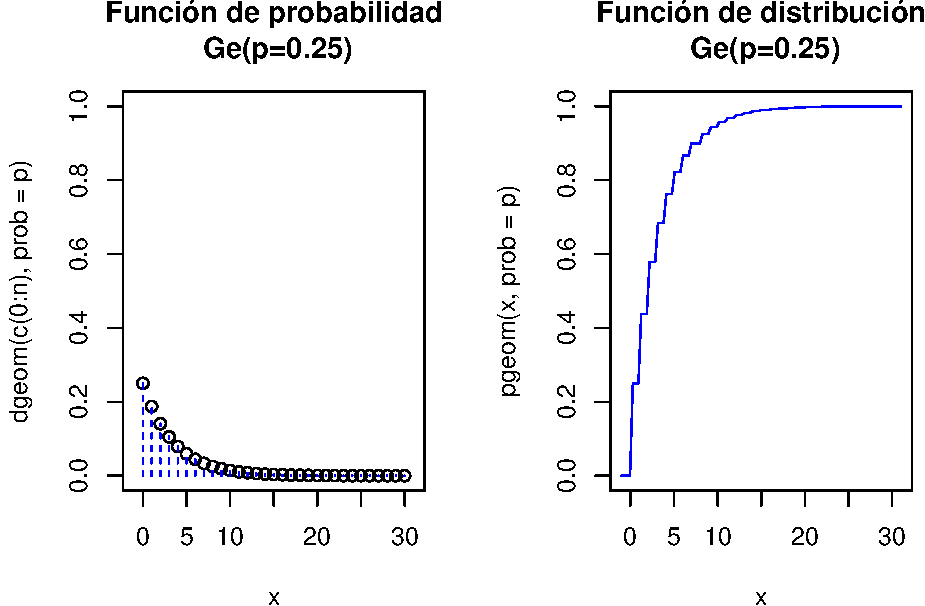
\includegraphics{curso-probabilidad-udemy_files/figure-latex/graficos22-1} \end{center}

\hypertarget{gruxe1ficas-interactivas-geomuxe9trica}{%
\subsection{Gráficas interactivas geométrica}\label{gruxe1ficas-interactivas-geomuxe9trica}}

Para ejecutar el siguiente gráfico interactivo, solamente tienes que cargar el paquete \texttt{shiny} en tu ordenador y luego copiar/pegar las siguientes instrucciones. De este modo podrás observar los cambios en las distribuciones variando los parámetros.

\begin{Shaded}
\begin{Highlighting}[]
\KeywordTok{sliderInput}\NormalTok{(}\StringTok{"p_geom"}\NormalTok{, }\DataTypeTok{label =} \StringTok{"Probabilidad de éxito:"}\NormalTok{,}
              \DataTypeTok{min =} \FloatTok{0.01}\NormalTok{, }\DataTypeTok{max =} \FloatTok{0.99}\NormalTok{, }\DataTypeTok{value =}\FloatTok{0.25}\NormalTok{ , }\DataTypeTok{step =} \FloatTok{0.01}\NormalTok{)}
\KeywordTok{renderPlot}\NormalTok{(\{}
  \KeywordTok{par}\NormalTok{(}\DataTypeTok{mfrow=}\KeywordTok{c}\NormalTok{(}\DecValTok{1}\NormalTok{,}\DecValTok{2}\NormalTok{))}
\NormalTok{  p=input}\OperatorTok{$}\NormalTok{p_geom}
\NormalTok{  n=}\DecValTok{30}
\NormalTok{  aux=}\KeywordTok{rep}\NormalTok{(}\DecValTok{0}\NormalTok{,(n}\OperatorTok{+}\DecValTok{1}\NormalTok{)}\OperatorTok{*}\DecValTok{2}\NormalTok{)}
\NormalTok{  aux[}\KeywordTok{seq}\NormalTok{(}\DecValTok{2}\NormalTok{,(n}\OperatorTok{+}\DecValTok{1}\NormalTok{)}\OperatorTok{*}\DecValTok{2}\NormalTok{,}\DecValTok{2}\NormalTok{)]=}\KeywordTok{dgeom}\NormalTok{(}\KeywordTok{c}\NormalTok{(}\DecValTok{0}\OperatorTok{:}\NormalTok{n),}\DataTypeTok{prob=}\NormalTok{p)}
  \KeywordTok{plot}\NormalTok{(}\DataTypeTok{x=}\KeywordTok{c}\NormalTok{(}\DecValTok{0}\OperatorTok{:}\NormalTok{n),}\DataTypeTok{y=}\KeywordTok{dgeom}\NormalTok{(}\KeywordTok{c}\NormalTok{(}\DecValTok{0}\OperatorTok{:}\NormalTok{n),}\DataTypeTok{prob=}\NormalTok{p),}
       \DataTypeTok{ylim=}\KeywordTok{c}\NormalTok{(}\DecValTok{0}\NormalTok{,}\DecValTok{1}\NormalTok{),}\DataTypeTok{xlim=}\KeywordTok{c}\NormalTok{(}\OperatorTok{-}\DecValTok{1}\NormalTok{,n}\OperatorTok{+}\DecValTok{1}\NormalTok{),}\DataTypeTok{xlab=}\StringTok{"x"}\NormalTok{,}
       \DataTypeTok{main=}\KeywordTok{paste0}\NormalTok{(}\KeywordTok{c}\NormalTok{(}\StringTok{"Función de probabilidad}\CharTok{\textbackslash{}n}\StringTok{ Ge(p="}\NormalTok{,p,}\StringTok{")"}\NormalTok{),}\DataTypeTok{collapse =} \StringTok{""}\NormalTok{))}
  \KeywordTok{lines}\NormalTok{(}\DataTypeTok{x=}\KeywordTok{rep}\NormalTok{(}\DecValTok{0}\OperatorTok{:}\NormalTok{n,}\DataTypeTok{each=}\DecValTok{2}\NormalTok{),}\DataTypeTok{y=}\NormalTok{aux, }\DataTypeTok{type =} \StringTok{"h"}\NormalTok{, }\DataTypeTok{lty =} \DecValTok{2}\NormalTok{,}\DataTypeTok{col=}\StringTok{"blue"}\NormalTok{)}
  \KeywordTok{curve}\NormalTok{(}\KeywordTok{pgeom}\NormalTok{(x,}\DataTypeTok{prob=}\NormalTok{p),}
        \DataTypeTok{xlim=}\KeywordTok{c}\NormalTok{(}\OperatorTok{-}\DecValTok{1}\NormalTok{,n}\OperatorTok{+}\DecValTok{1}\NormalTok{),}\DataTypeTok{col=}\StringTok{"blue"}\NormalTok{,}
        \DataTypeTok{main=}\KeywordTok{paste0}\NormalTok{(}\KeywordTok{c}\NormalTok{(}\StringTok{"Función de distribución\textbackslash{}n Ge(p="}\NormalTok{,p,}\StringTok{")"}\NormalTok{),}\DataTypeTok{collapse =} \StringTok{""}\NormalTok{))}
  \KeywordTok{par}\NormalTok{(}\DataTypeTok{mfrow=}\KeywordTok{c}\NormalTok{(}\DecValTok{1}\NormalTok{,}\DecValTok{1}\NormalTok{))}
\NormalTok{\})}
\end{Highlighting}
\end{Shaded}

\href{https://joanby.shinyapps.io/DistribucionesNotables/}{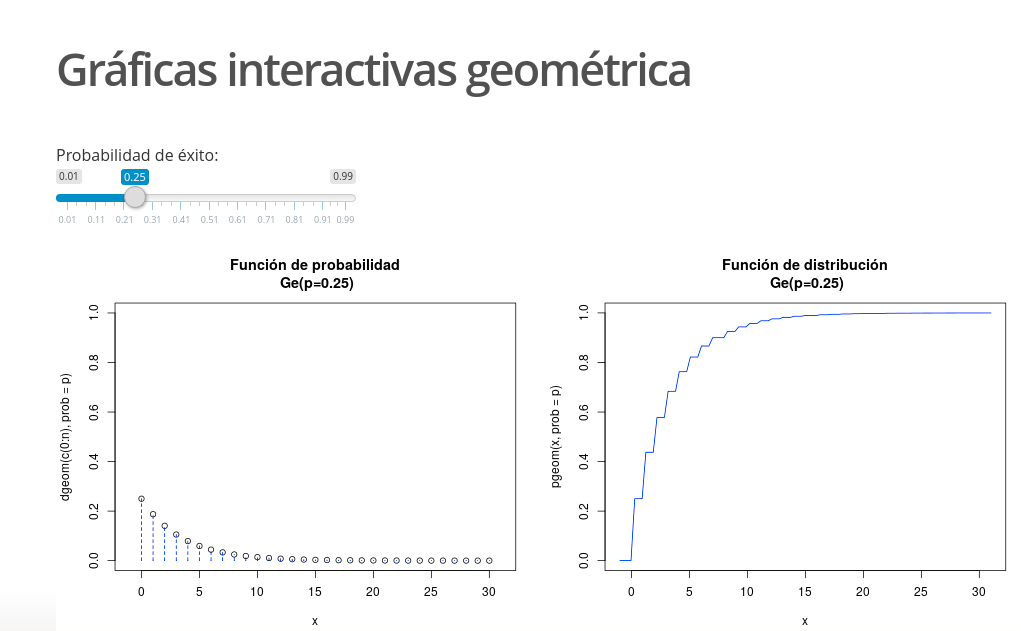
\includegraphics{Images/noshinyImages/interactiva_geometrica1.png}}

\hypertarget{cuxe1lculos-con-python}{%
\subsection{Cálculos con python}\label{cuxe1lculos-con-python}}

Veamos los cálculos básicos con python para la distribución geométrica \(Ge(p=0.25)\). scipy.stats implementa la distribución geométrica que cuenta el número intentos así que empieza en 1.

Cargamos la función de la librería

\begin{Shaded}
\begin{Highlighting}[]
\ImportTok{from}\NormalTok{ scipy.stats }\ImportTok{import}\NormalTok{ geom}
\end{Highlighting}
\end{Shaded}

\hypertarget{cuxe1lculos-con-python-1}{%
\subsection{Cálculos con python}\label{cuxe1lculos-con-python-1}}

La función de probabilidad es \texttt{geom.pmf(x,p,loc=0)=geom.pmf(x,p)} es un geométrica que cuenta el número de intentos para obtener el primer éxito el valor por defecto del último parámetro es \texttt{loc=0}.

Si queremos la que cuenta el número de fracasos para obtener el primer éxito (la geométrica que empieza en 0) tenemos que usar \texttt{geom.pmf(x,p,loc=-1)}.

Es decir \texttt{geom.pmf(x,p,loc=-1)=geom.pmf(x-1,p,loc=0)}

\hypertarget{cuxe1lculos-con-python-2}{%
\subsection{Cálculos con python}\label{cuxe1lculos-con-python-2}}

Veamos pues los cálculos para la \(Ge(p)\) que empieza en \(0\).

\(P(X=0)=(1-0.25)^0\cdot 0.25^1=0.25\)

\begin{Shaded}
\begin{Highlighting}[]
\NormalTok{geom.pmf(}\DecValTok{0}\NormalTok{,p}\OperatorTok{=}\FloatTok{0.25}\NormalTok{,loc}\OperatorTok{=-}\DecValTok{1}\NormalTok{)}
\end{Highlighting}
\end{Shaded}

\begin{verbatim}
## 0.25
\end{verbatim}

\(P(X\leq 0)=1- (1-0.25)^{0+1}=1-0.75=0.25\)

\begin{Shaded}
\begin{Highlighting}[]
\NormalTok{geom.cdf(}\DecValTok{0}\NormalTok{,p}\OperatorTok{=}\FloatTok{0.25}\NormalTok{,loc}\OperatorTok{=-}\DecValTok{1}\NormalTok{)}
\end{Highlighting}
\end{Shaded}

\begin{verbatim}
## 0.25
\end{verbatim}

\hypertarget{cuxe1lculos-con-python-3}{%
\subsection{Cálculos con python}\label{cuxe1lculos-con-python-3}}

\(P(X\leq 4)=1-(1-0.25)^{4+1}=1-0.75=1-0.75^5=0.7626953.\)

\begin{Shaded}
\begin{Highlighting}[]
\NormalTok{geom.cdf(}\DecValTok{4}\NormalTok{,p}\OperatorTok{=}\FloatTok{0.25}\NormalTok{,loc}\OperatorTok{=-}\DecValTok{1}\NormalTok{)}
\end{Highlighting}
\end{Shaded}

\begin{verbatim}
## 0.7626953125
\end{verbatim}

Una muestra aleatoria de tamaño 25 de una \(Ge(0.25)\)

\begin{Shaded}
\begin{Highlighting}[]
\NormalTok{geom.rvs(p}\OperatorTok{=}\FloatTok{0.25}\NormalTok{, size}\OperatorTok{=}\DecValTok{20}\NormalTok{, loc}\OperatorTok{=-}\DecValTok{1}\NormalTok{)}
\end{Highlighting}
\end{Shaded}

\begin{verbatim}
## array([ 2,  1,  4,  8,  0,  2,  5,  0,  1,  1,  2,  3,  4,  0,  8,  0,  1,
##        18,  7,  4])
\end{verbatim}

\hypertarget{cuxe1lculos-con-python-4}{%
\subsection{Cálculos con python}\label{cuxe1lculos-con-python-4}}

\textbf{Ejercicio}

Qué probabilidades son las que calcula el siguiente código y qué tipo de variables geométricas son?

\begin{Shaded}
\begin{Highlighting}[]
\NormalTok{geom.cdf(}\BuiltInTok{range}\NormalTok{(}\DecValTok{5}\NormalTok{),p}\OperatorTok{=}\FloatTok{0.3}\NormalTok{,loc}\OperatorTok{=}\DecValTok{0}\NormalTok{)}
\end{Highlighting}
\end{Shaded}

\begin{verbatim}
## array([ 0.    ,  0.3   ,  0.51  ,  0.657 ,  0.7599])
\end{verbatim}

\begin{Shaded}
\begin{Highlighting}[]
\NormalTok{geom.cdf(}\BuiltInTok{range}\NormalTok{(}\DecValTok{5}\NormalTok{),p}\OperatorTok{=}\FloatTok{0.3}\NormalTok{,loc}\OperatorTok{=-}\DecValTok{1}\NormalTok{)}
\end{Highlighting}
\end{Shaded}

\begin{verbatim}
## array([ 0.3    ,  0.51   ,  0.657  ,  0.7599 ,  0.83193])
\end{verbatim}

\hypertarget{cuxe1lculos-con-python-esperanza-y-varianza}{%
\subsection{Cálculos con python esperanza y varianza}\label{cuxe1lculos-con-python-esperanza-y-varianza}}

Con python también podemos calcular directamente algunos parámetros asociado a una función de distribución predefinida

\begin{Shaded}
\begin{Highlighting}[]
\NormalTok{geom.stats(p}\OperatorTok{=}\FloatTok{0.25}\NormalTok{, loc}\OperatorTok{=}\DecValTok{0}\NormalTok{, moments}\OperatorTok{=}\StringTok{'mv'}\NormalTok{)}
\end{Highlighting}
\end{Shaded}

\begin{verbatim}
## (array(4.0), array(12.0))
\end{verbatim}

\begin{Shaded}
\begin{Highlighting}[]
\NormalTok{geom.stats(p}\OperatorTok{=}\FloatTok{0.25}\NormalTok{, loc}\OperatorTok{=-}\DecValTok{1}\NormalTok{, moments}\OperatorTok{=}\StringTok{'mv'}\NormalTok{)}
\end{Highlighting}
\end{Shaded}

\begin{verbatim}
## (array(3.0), array(12.0))
\end{verbatim}

\hypertarget{cuxe1lculos-con-python-esperanza-y-varianza-1}{%
\subsection{Cálculos con python esperanza y varianza}\label{cuxe1lculos-con-python-esperanza-y-varianza-1}}

\textbf{Ejercicio}

Comprobad que las medias y las varianzas calculadas en el código anterior, corresponden a una \(Ge(p=0.3)\) empezando en \(1\) y a a un \(Ge(p=0.3)\)
empezando en \(0\).

¿Son las varianzas siempre iguales?

\hypertarget{gruxe1ficos-con-python}{%
\subsection{Gráficos con python}\label{gruxe1ficos-con-python}}

\begin{Shaded}
\begin{Highlighting}[]
\NormalTok{p }\OperatorTok{=} \FloatTok{0.25}
\NormalTok{x }\OperatorTok{=}\NormalTok{ np.arange(geom.ppf(}\FloatTok{0.01}\NormalTok{, p),geom.ppf(}\FloatTok{0.99}\NormalTok{, p))}
\NormalTok{fig }\OperatorTok{=}\NormalTok{plt.figure(figsize}\OperatorTok{=}\NormalTok{(}\DecValTok{5}\NormalTok{, }\FloatTok{2.7}\NormalTok{))}
\NormalTok{ax }\OperatorTok{=}\NormalTok{ fig.add_subplot(}\DecValTok{1}\NormalTok{,}\DecValTok{2}\NormalTok{,}\DecValTok{1}\NormalTok{)}
\NormalTok{ax.plot(x, geom.pmf(x, p), }\StringTok{'bo'}\NormalTok{, ms}\OperatorTok{=}\DecValTok{5}\NormalTok{, label}\OperatorTok{=}\StringTok{'geom pmf'}\NormalTok{)}
\NormalTok{ax.vlines(x, }\DecValTok{0}\NormalTok{, geom.pmf(x, p), colors}\OperatorTok{=}\StringTok{'b'}\NormalTok{, lw}\OperatorTok{=}\DecValTok{2}\NormalTok{, alpha}\OperatorTok{=}\FloatTok{0.5}\NormalTok{)}
\ControlFlowTok{for}\NormalTok{ tick }\KeywordTok{in}\NormalTok{ ax.xaxis.get_major_ticks():}
\NormalTok{  tick.label.set_fontsize(}\DecValTok{5}\NormalTok{)}
\ControlFlowTok{for}\NormalTok{ tick }\KeywordTok{in}\NormalTok{ ax.yaxis.get_major_ticks():}
\NormalTok{  tick.label.set_fontsize(}\DecValTok{5}\NormalTok{) }
\NormalTok{ax }\OperatorTok{=}\NormalTok{ fig.add_subplot(}\DecValTok{1}\NormalTok{,}\DecValTok{2}\NormalTok{,}\DecValTok{2}\NormalTok{)}
\NormalTok{ax.plot(x, geom.cdf(x, p), }\StringTok{'bo'}\NormalTok{, ms}\OperatorTok{=}\DecValTok{5}\NormalTok{, label}\OperatorTok{=}\StringTok{'geom pmf'}\NormalTok{)}
\NormalTok{ax.vlines(x, }\DecValTok{0}\NormalTok{, geom.cdf(x, p), colors}\OperatorTok{=}\StringTok{'b'}\NormalTok{, lw}\OperatorTok{=}\DecValTok{2}\NormalTok{, alpha}\OperatorTok{=}\FloatTok{0.5}\NormalTok{)}
\ControlFlowTok{for}\NormalTok{ tick }\KeywordTok{in}\NormalTok{ ax.xaxis.get_major_ticks():}
\NormalTok{  tick.label.set_fontsize(}\DecValTok{5}\NormalTok{)}
\ControlFlowTok{for}\NormalTok{ tick }\KeywordTok{in}\NormalTok{ ax.yaxis.get_major_ticks():}
\NormalTok{  tick.label.set_fontsize(}\DecValTok{5}\NormalTok{)}
\NormalTok{fig.suptitle(}\StringTok{'Distribucion Geometrica'}\NormalTok{)}
\NormalTok{plt.show()}
\end{Highlighting}
\end{Shaded}

\hypertarget{gruxe1ficos-con-python-1}{%
\subsection{Gráficos con python}\label{gruxe1ficos-con-python-1}}

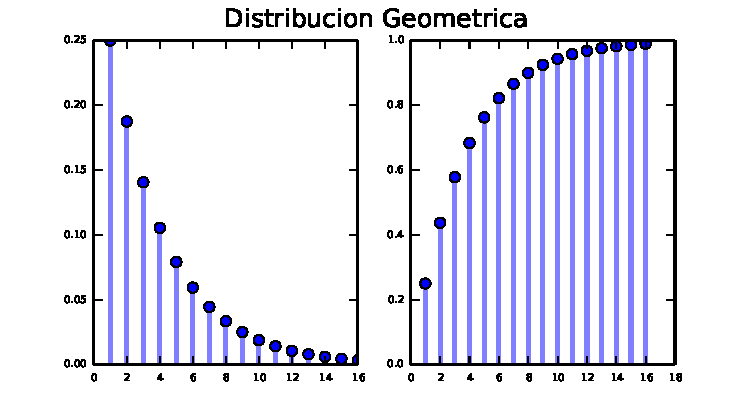
\includegraphics{curso-probabilidad-udemy_files/figure-latex/unnamed-chunk-35-1.pdf}

\hypertarget{distribuciuxf3n-binomial-negativa}{%
\section{Distribución binomial negativa}\label{distribuciuxf3n-binomial-negativa}}

\hypertarget{el-problema-de-la-puerta-con-dos-cerraduras}{%
\subsection{El problema de la puerta con dos cerraduras}\label{el-problema-de-la-puerta-con-dos-cerraduras}}

Supongamos que disponemos de 10 llaves distintas y tenemos que abrir una puerta con \textbf{dos cerraduras}.

Comenzamos por la primera cerradura, de tal forma que cada vez olvidamos que llave que hemos probado.

Una vez abierta la primera cerradura probamos de igual forma con la segunda hasta que también la abrimos.

Sea \(X=\) la v.a. que cuenta el número de fracasos hasta abrir la puerta.

Acertar una llave de la puerta es un experimento Bernoulli con probabilidad de éxito \(p=0.1\). Lo repetiremos hasta obtener 2 éxitos.

\hypertarget{distribuciuxf3n-binomial-negativa-1}{%
\subsection{Distribución binomial negativa}\label{distribuciuxf3n-binomial-negativa-1}}

En general tendremos un experimento Bernoulli con probabilidad de éxito \(0<p<1\) y tal que:

\begin{itemize}
\tightlist
\item
  Repetimos el experimento hasta obtener el \(n\)-ésimo éxito ¡¡abrir la maldita puerta!!.
\item
  Sea \(X\) la v.a que cuenta el número fallos hasta abrir la puerta, es decir, hasta conseguir el n-ésimo éxito. Notemos que no contamos los éxitos, solo contamos los fracasos
\end{itemize}

\hypertarget{distribuciuxf3n-binomial-negativa-2}{%
\subsection{Distribución binomial negativa}\label{distribuciuxf3n-binomial-negativa-2}}

Si representamos como es habitual un suceso son una cadena de F's y E's.

Si \(n=2\) estos son algunos sucesos elementales
\[\{EE,FEE,EFE, FFEE,FEFE,EFFE,FFFEE,FFEFE,FEFFE,EFFFE\}\]

\[P(X=0)=P(\{EE\})=p^2\]

\[P(X=1)=P(\{FEE,EFE\})=2\cdot (1-p)\cdot p^2\]
\[P(X=2)=P(\{FFEE,FEFE,EFFE\})=3\cdot (1-p) 2\cdot p^2\]

\[P(X=3)=P(\{FFFEE,FFEFE,FEFFE,EFFFE\})=4\cdot (1-p)^3\cdot p^2\]

\hypertarget{distribuciuxf3n-binomial-negativa-3}{%
\subsection{Distribución binomial negativa}\label{distribuciuxf3n-binomial-negativa-3}}

En general su función de probabilidad es

\[
P_{X}(k)=P(X=k)=\left\{\begin{array}{ll}
     {{k+n-1}\choose{n-1}} \cdot (1-p)^{k}\cdot p^n & \mbox{si } k=0,1,\ldots\\
     0 & \mbox{en otro caso}\end{array}\right.
\]

\hypertarget{distribuciuxf3n-binomial-negativa-4}{%
\subsection{Distribución binomial negativa}\label{distribuciuxf3n-binomial-negativa-4}}

Una v.a. con este tipo de distribución recibe el nombre de \emph{binomial negativa} y la denotaremos por \(BN(n,p)\).

Notemos que \(BN(1,p)=Ge(p)\).

\hypertarget{distribuciuxf3n-binomial-negativa-5}{%
\subsection{Distribución binomial negativa}\label{distribuciuxf3n-binomial-negativa-5}}

\textbf{Demostración}

Justifiquemos el resultado. Sea \(X\) una \(BN(n,p)\) y sea \(k=0,1,2,\ldots\).

\[P(X=k)=P(\mbox{Todas las cadenas de E's y F' con $k$ F, con $n$ E y acabadas en E})\]

\[
\overbrace{\underbrace{\overbrace{EFFF\ldots EEF}^{n-1 \quad \mbox{Éxitos}.}}}_{k \quad\mbox{Fracasos}}^{k+n-1\mbox{ posiciones}}E
\]

De estas cadenas hay tantas como maneras de elegir de entre las \(k+n-1\) primeras posiciones \(n-1\) para colocar los éxitos, esta cantidad es el número binomial

\[{k+n-1\choose n-1}\]

\hypertarget{nuxfameros-binomiales-negativos}{%
\subsection{Números binomiales negativos}\label{nuxfameros-binomiales-negativos}}

 Números binomiales negativos

Dados dos enteros positivos \(n\) y \(k\) se define en numero binomial negativo como

\[\binom{-n}{k}=\frac{(-n)(-n-1)\cdots (-n-k+1)}{k!}.\]

Se cumple que

\[
(t+1)^{-n}=\sum_{k=0}^{+\infty}\left(\begin{array}{c} -n
\\ k\end{array}\right) t^{k}
\]

\hypertarget{nuxfameros-binomiales-negativos-1}{%
\subsection{Números binomiales negativos}\label{nuxfameros-binomiales-negativos-1}}

Con R es la misma función que para los números binomiales

\[
\begin{eqnarray*}
{-6\choose 4}&=&\frac{-6\cdot (-6-1)\cdot \cdot (-6-2)\cdot (-6-3) }{4!}\\
&=&  \frac{-6\cdot(-7)\cdot (-8)\cdot (-9)}{24}\\
&=& \frac{3024}{24}=126.
\end{eqnarray*}
\]

Efectivamente obtenemos el mismo resultado

\begin{Shaded}
\begin{Highlighting}[]
\KeywordTok{choose}\NormalTok{(}\OperatorTok{-}\DecValTok{6}\NormalTok{,}\DecValTok{4}\NormalTok{)}
\end{Highlighting}
\end{Shaded}

\begin{verbatim}
## [1] 126
\end{verbatim}

\hypertarget{esperanza-de-una-bnnp}{%
\subsection{\texorpdfstring{Esperanza de una \(BN(n,p)\)}{Esperanza de una BN(n,p)}}\label{esperanza-de-una-bnnp}}

Su \textbf{esperanza es}

\[E(X)=\displaystyle\sum_{k=0}^{+\infty} k\cdot {k+n-1\choose n-1} \cdot (1-p)^{k}\cdot p^n=n\cdot\frac{1-p}{p}.\]

La \textbf{esperanza del cuadrado \(X^2\) es}

\[E(X^2)=\displaystyle\sum_{k=0}^{+\infty} k^2\cdot {k+n-1\choose n-1} \cdot (1-p)^{k}\cdot p^n=n\cdot\frac{1-p}{p^2}+\left(n\cdot \frac{1-p}{p}\right)^2.\]

\hypertarget{varianza-de-una-bnnp}{%
\subsection{\texorpdfstring{Varianza de una \(BN(n,p)\)}{Varianza de una BN(n,p)}}\label{varianza-de-una-bnnp}}

Por último la \textbf{varianza es}

\[
Var(X)=E(X^2)-E(X)^2=
\]

\[=n\cdot \frac{1-p}{p^2}+\left(n\cdot \frac{1-p}{p}\right)^2-\left(n\cdot \frac{1-p}{p}\right)^2=
n\cdot \frac{1-p}{p^2}.\]

y por tanto la desviación típica es

\[\sqrt{Var(X)} = \frac{\sqrt{n(1-p)}}{p}\]

\hypertarget{resumen-binomial-negativa-bnnp}{%
\subsection{\texorpdfstring{Resumen Binomial Negativa \(BN(n,p)\)}{Resumen Binomial Negativa BN(n,p)}}\label{resumen-binomial-negativa-bnnp}}

\begin{longtable}[]{@{}rl@{}}
\toprule
\begin{minipage}[b]{0.50\columnwidth}\raggedleft
\(X\), \(BN(n,p)\)\strut
\end{minipage} & \begin{minipage}[b]{0.44\columnwidth}\raggedright
Número de fracasos antes de conseguir el \(n\)-ésimo éxito. Probabilidad de éxito \(p\)\strut
\end{minipage}\tabularnewline
\midrule
\endhead
\begin{minipage}[t]{0.50\columnwidth}\raggedleft
\(D_X=\)\strut
\end{minipage} & \begin{minipage}[t]{0.44\columnwidth}\raggedright
\(\{0,1,2,3\ldots\}\)\strut
\end{minipage}\tabularnewline
\begin{minipage}[t]{0.50\columnwidth}\raggedleft
\(P_X(k)=P(X=k)=\)\strut
\end{minipage} & \begin{minipage}[t]{0.44\columnwidth}\raggedright
\(\left\{\begin{array}{ll} {k+n-1\choose n-1} \cdot (1-p)^{k}\cdot p^n & \mbox{si } k=0,1,\ldots \\ 0 & \mbox{en otro caso.}\end{array}\right.\)\strut
\end{minipage}\tabularnewline
\begin{minipage}[t]{0.50\columnwidth}\raggedleft
\(F_X(x)=P(X\leq X)=\)\strut
\end{minipage} & \begin{minipage}[t]{0.44\columnwidth}\raggedright
\(\begin{array}{l}\left\{\begin{array}{ll} 0 & \mbox{si } x<0\\\displaystyle\sum_{i=0}^{k} P(X=i) & \mbox{si }\left\{\begin{array}{l}k\leq x< k+1\\k=0,1,2,\ldots\end{array}\right.\end{array}\right. \\\mbox{Calcular la suma o utilizar funciones de R o python.} \end{array}\)\strut
\end{minipage}\tabularnewline
\begin{minipage}[t]{0.50\columnwidth}\raggedleft
\(E(X)=n\cdot\frac{1-p}{p}\)\strut
\end{minipage} & \begin{minipage}[t]{0.44\columnwidth}\raggedright
\(Var(X)=n\cdot \frac{1-p}{p^2}\)\strut
\end{minipage}\tabularnewline
\bottomrule
\end{longtable}

\hypertarget{ejemplo-puerta-dos-cerraduras-bnn2p0.1.}{%
\subsection{\texorpdfstring{Ejemplo puerta dos cerraduras \(BN(n=2,p=0.1)\).}{Ejemplo puerta dos cerraduras BN(n=2,p=0.1).}}\label{ejemplo-puerta-dos-cerraduras-bnn2p0.1.}}

\textbf{Ejercicio: Puerta con dos cerraduras}

Recordemos nuestra puerta con dos cerraduras que se abren secuencialmente. Tenemos un manojo de 10 llaves casi idénticas. De manera que cada vez que probamos una llave olvidamos qué llave hemos usado.

Sea \(X\) la v.a que nos da el número de intentos fallidos hasta abrir abrir la puerta.

\hypertarget{ejemplo-bnnp}{%
\subsection{\texorpdfstring{Ejemplo \(BN(n,p)\)}{Ejemplo BN(n,p)}}\label{ejemplo-bnnp}}

Estamos interesado en modelar este problema. La preguntas son:

\begin{enumerate}
\def\labelenumi{\arabic{enumi}.}
\tightlist
\item
  ¿Cuál es la distribución de probabilidad de \(X\) la v.a que nos da el número fallos hasta abrir la puerta?
\item
  ¿Cuál es la función de probabilidad y de distribución del \(X\)?
\item
  ¿Cuál es la probabilidad de fallar exactamente 5 veces antes de abrir la puerta?
\item
  ¿Cuál es la probabilidad de fallar más de 4?
\item
  ¿Cuál es el número esperado de fallos? ¿Y su desviación típica?
\end{enumerate}

\hypertarget{ejemplo-dos-cerraduras-bnn2p0.1.}{%
\subsection{\texorpdfstring{Ejemplo dos cerraduras \(BN(n=2,p=0.1)\).}{Ejemplo dos cerraduras BN(n=2,p=0.1).}}\label{ejemplo-dos-cerraduras-bnn2p0.1.}}

\textbf{Solución 1.} ¿Cuál es la distribución de probabilidad de \(X\) la v.a que nos da el número fallos hasta abrir la puerta?

Bajo estados condiciones tenemos que la probabilidad de ``éxito'' de cada intento es \(p=\frac{1}{10}=.01\). Como cada vez \emph{olvidamos} qué llave hemos probado cada intento será independiente del anterior.

Así que la variable \(X\) que queremos modelar cuenta el número fallos de repeticiones sucesivas e independientes de un experimento \(Ber(p=0.1)\) hasta conseguir 2 éxitos en un experimento.

Por lo tanto podemos asegurar que \(X\) sigue un distribución \(BN(n=2,p=0.1).\)

\hypertarget{ejemplo-bnn2p0.1}{%
\subsection{\texorpdfstring{Ejemplo \(BN(n=2,p=0.1)\)}{Ejemplo BN(n=2,p=0.1)}}\label{ejemplo-bnn2p0.1}}

\textbf{Solución 2.} ¿Cuál es la función de probabilidad y de distribución del \(X\)?

En general la función de probabilidad de una \(BN(n,p)\) es

\[
P_X(X=k)=P(X=k)=
\left\{
\begin{array}{cc} 
{k+n-1\choose n-1} \cdot (1-p)^{k}\cdot p^n & \mbox{si }  k=0,1,\ldots \\ 0 & \mbox{en otro caso.}\end{array}\right.
\]
En particular la función de probabilidad de una \(BN(n=2,p=0.1)\) es

\[
P_X(X=k)=P(X=k)=
\left\{
\begin{array}{cc} 
{k+2-1\choose 2-1} \cdot 0.9^{k}\cdot 0.1^2 & \mbox{si }  k=0,1,2,\ldots \\ 0 & \mbox{en otro caso.}\end{array}\right.
\]

\hypertarget{ejemplo-bnn2p0.1-1}{%
\subsection{\texorpdfstring{Ejemplo \(BN(n=2,p=0.1)\)}{Ejemplo BN(n=2,p=0.1)}}\label{ejemplo-bnn2p0.1-1}}

Simplificando

\[
P_X(X=k)=P(X=k)=
\left\{
\begin{array}{cc} 
{k+1\choose 1} \cdot 0.9^{k}\cdot 0.1^2 & \mbox{si }  k=0,1,2,\ldots \\ 0 & \mbox{en otro caso.}\end{array}\right.
\]

\hypertarget{ejemplo-bnn2p0.1-2}{%
\subsection{\texorpdfstring{Ejemplo \(BN(n=2,p=0.1)\)}{Ejemplo BN(n=2,p=0.1)}}\label{ejemplo-bnn2p0.1-2}}

La función de distribución en general es

\[
F_x(x)=P(X\leq x)=
\left\{
\begin{array}{ll}
0 & \mbox{si } x<0 \\
\displaystyle\sum_{i=0}^{k }{i+n-1\choose n-1} \cdot (1-p)^{i+n-1}\cdot p^n 
& \mbox{si }\left\{\begin{array}{l} k\leq x< k+1\\k=0,1,2,\ldots\end{array}\right. 
\end{array}
\right.
\]

\hypertarget{ejemplo-bnn2p0.1-3}{%
\subsection{\texorpdfstring{Ejemplo \(BN(n=2,p=0.1)\)}{Ejemplo BN(n=2,p=0.1)}}\label{ejemplo-bnn2p0.1-3}}

Simplificando para \(n=2\), \(p=0.1\).

\[
F_x(x)=P(X\leq x)=
\left\{
\begin{array}{ll}
0 & \mbox{si } x<0 \\
\displaystyle\sum_{i=0}^{k }{i+1\choose 1} \cdot 0.9^{i+1}\cdot 0.1^2
& \mbox{si }\left\{\begin{array}{l} k\leq x< k+1\\k=0,1,2,\ldots\end{array}\right. 
\end{array}
\right.
\]

\hypertarget{ejemplo-bnn2p0.1-4}{%
\subsection{\texorpdfstring{Ejemplo \(BN(n=2,p=0.1)\)}{Ejemplo BN(n=2,p=0.1)}}\label{ejemplo-bnn2p0.1-4}}

\textbf{Solución 3.} ¿Cuál es la probabilidad de fallar exactamente 5 veces antes de abrir la puerta?

\[
\begin{eqnarray*}
P(X=5)&=&{5+2-1\choose 1} \cdot 0.9^{5}\cdot 0.1^2= {6\choose 1} \cdot 0.9^{5}\cdot 0.1^2\\
&=& 6\cdot 0.9^5\cdot 0.1^2= 0.0354294.
\end{eqnarray*}
\]

\hypertarget{ejemplo-bnn2p0.1-5}{%
\subsection{\texorpdfstring{Ejemplo \(BN(n=2,p=0.1)\)}{Ejemplo BN(n=2,p=0.1)}}\label{ejemplo-bnn2p0.1-5}}

\textbf{Solución 4.} ¿Cuál es la probabilidad de fallar más de 4

Nos piden que\\
\[
P(X>4)=1-P(X\leq 4).
\]

Calculemos primero \(P(X\leq 4):\)

\[
\begin{eqnarray*}
P(X\leq 4) &= & \displaystyle\sum_{x=0}^{4} P(X=x)=P(X=0)+P(X=1)+P(X=2)+P(X=3)+P(X=4)\\
&=& {0+2-1\choose 1} \cdot 0.9^{0}\cdot 0.1^2+
    {1+2-1\choose 1} \cdot 0.9^{1}\cdot 0.1^2\\
  &+&
    {2+2-1\choose 1} \cdot 0.9^{2}\cdot 0.1^2+
    {3+2-1\choose 1} \cdot 0.9^{3}\cdot 0.1^2 \\ 
  &+&
    {4+2-1\choose 1} \cdot 0.9^{4}\cdot 0.1^2=\ldots
\end{eqnarray*}
\]

\hypertarget{ejemplo-bnn2p0.1-6}{%
\subsection{\texorpdfstring{Ejemplo \(BN(n=2,p=0.1)\)}{Ejemplo BN(n=2,p=0.1)}}\label{ejemplo-bnn2p0.1-6}}

\[
\begin{eqnarray*}
P(X\leq 4)=\ldots   &=& 
{1\choose 1} \cdot 0.9^{0}\cdot 0.1^2+
{2\choose 1} \cdot 0.9^{1}\cdot 0.1^2+  
{3\choose 1} \cdot 0.9^{2}\cdot 0.1^2+
{4\choose 1} \cdot 0.9^{3}\cdot 0.1^2\\ 
  &+&
{5\choose 1} \cdot 0.9^{4}\cdot 0.1^2=
0.1^2+
2\cdot 0.9 \cdot 0.1^2+
3\cdot 0.9^2\cdot 0.1^2+
4\cdot 0.9^3\cdot 0.1^2+
5\cdot 0.9^4\cdot 0.1^2\\
=
0.114265
\end{eqnarray*}.
\]

Por lo tanto

\[
P(X>4)=1-P(X\leq 4)=1-0.114265=
0.885735.
\]

\hypertarget{ejemplo-bnn2p0.1-7}{%
\subsection{\texorpdfstring{Ejemplo \(BN(n=2,p=0.1)\)}{Ejemplo BN(n=2,p=0.1)}}\label{ejemplo-bnn2p0.1-7}}

\textbf{Solución 5.} ¿Cuál es el número esperado de fallos? ¿Y su desviación típica?

Como \(X\) sigue una ley \(BN(n=2,p=0.1)\)

\[E(X)=n\cdot \frac{1-p}{p}=2\cdot \frac{1-0.1}{0.1}=18.\]

El número de fallos esperado es 18.

\[
Var(X)=n\cdot\frac{1-p}{p^2}=2 \cdot \frac{1-0.1}{0.1^2}=180.
\]

La varianza de \(X\) es 180 y su desviación típica \(\sqrt{180}=13.41641.\)

\hypertarget{cuxe1lculos-con-r-2}{%
\subsection{Cálculos con R}\label{cuxe1lculos-con-r-2}}

La función de R para la función de probabilidad de la binomial negativa y sus parámetros básicos son

\begin{verbatim}
dnbinom(x, size, prob,...)`
\end{verbatim}

Donde \texttt{size} (\(n\)) es el número de éxitos y \texttt{prob} (\(p\)) la probabilidad de éxito.

Así en el ejemplo de la puerta \(X\) es una \(BN(n=size=2,p=prob=0.1)\). Por ejemplo \(P(X=5)\) que hemos calculado en el ejemplo anterior es

\begin{Shaded}
\begin{Highlighting}[]
\KeywordTok{dnbinom}\NormalTok{(}\DecValTok{5}\NormalTok{,}\DataTypeTok{size=}\DecValTok{2}\NormalTok{,}\DataTypeTok{p=}\FloatTok{0.1}\NormalTok{)}
\end{Highlighting}
\end{Shaded}

\begin{verbatim}
## [1] 0.0354294
\end{verbatim}

\hypertarget{cuxe1lculos-con-r-3}{%
\subsection{Cálculos con R}\label{cuxe1lculos-con-r-3}}

De forma similar calculamos calculamos \(P(X\leq 4)\), \(P(X>4)=1-P(X\leq 4)\) y \(P(X>4)\).

\begin{Shaded}
\begin{Highlighting}[]
\KeywordTok{pnbinom}\NormalTok{(}\DecValTok{4}\NormalTok{,}\DataTypeTok{size=}\DecValTok{2}\NormalTok{,}\DataTypeTok{p=}\FloatTok{0.1}\NormalTok{)}
\end{Highlighting}
\end{Shaded}

\begin{verbatim}
## [1] 0.114265
\end{verbatim}

\begin{Shaded}
\begin{Highlighting}[]
\DecValTok{1}\OperatorTok{-}\KeywordTok{pnbinom}\NormalTok{(}\DecValTok{4}\NormalTok{,}\DataTypeTok{size=}\DecValTok{2}\NormalTok{,}\DataTypeTok{p=}\FloatTok{0.1}\NormalTok{)}
\end{Highlighting}
\end{Shaded}

\begin{verbatim}
## [1] 0.885735
\end{verbatim}

\begin{Shaded}
\begin{Highlighting}[]
\KeywordTok{pnbinom}\NormalTok{(}\DecValTok{4}\NormalTok{,}\DataTypeTok{size=}\DecValTok{2}\NormalTok{,}\DataTypeTok{p=}\FloatTok{0.1}\NormalTok{,}\DataTypeTok{lower.tail=}\OtherTok{FALSE}\NormalTok{)}
\end{Highlighting}
\end{Shaded}

\begin{verbatim}
## [1] 0.885735
\end{verbatim}

\hypertarget{cuxe1lculos-con-python-5}{%
\subsection{Cálculos con python}\label{cuxe1lculos-con-python-5}}

La función con python es \texttt{nbinom.pmf(k,\ n,\ p,\ loc)}. Hay que cargarla desde \texttt{scpi.stats}

\begin{Shaded}
\begin{Highlighting}[]
\ImportTok{from}\NormalTok{ scipy.stats }\ImportTok{import}\NormalTok{ nbinom}
\end{Highlighting}
\end{Shaded}

Recordemos que de nuevo se cumple que

\begin{Shaded}
\begin{Highlighting}[]
\NormalTok{nbinom.pmf(k, n, p, loc) }\OperatorTok{=}\NormalTok{ nbinom.pmf(k}\OperatorTok{-}\NormalTok{loc, n, p)`}
\end{Highlighting}
\end{Shaded}

\hypertarget{cuxe1lculos-bnnp-con-python}{%
\subsection{\texorpdfstring{Cálculos \(BN(n,p)\) con python}{Cálculos BN(n,p) con python}}\label{cuxe1lculos-bnnp-con-python}}

\begin{Shaded}
\begin{Highlighting}[]
\NormalTok{nbinom.pmf(k}\OperatorTok{=}\DecValTok{5}\NormalTok{,n}\OperatorTok{=}\DecValTok{2}\NormalTok{,p}\OperatorTok{=}\FloatTok{0.1}\NormalTok{)}
\end{Highlighting}
\end{Shaded}

\begin{verbatim}
## 0.035429400000000041
\end{verbatim}

\begin{Shaded}
\begin{Highlighting}[]
\NormalTok{nbinom.pmf(k}\OperatorTok{=}\DecValTok{5}\NormalTok{,n}\OperatorTok{=}\DecValTok{2}\NormalTok{,p}\OperatorTok{=}\FloatTok{0.1}\NormalTok{,loc}\OperatorTok{=}\DecValTok{0}\NormalTok{)}
\end{Highlighting}
\end{Shaded}

\begin{verbatim}
## 0.035429400000000041
\end{verbatim}

\begin{Shaded}
\begin{Highlighting}[]
\NormalTok{nbinom.cdf(k}\OperatorTok{=}\DecValTok{4}\NormalTok{,n}\OperatorTok{=}\DecValTok{2}\NormalTok{,p}\OperatorTok{=}\FloatTok{0.1}\NormalTok{)}
\end{Highlighting}
\end{Shaded}

\begin{verbatim}
## 0.11426500000000003
\end{verbatim}

\begin{Shaded}
\begin{Highlighting}[]
\DecValTok{1}\OperatorTok{-}\NormalTok{nbinom.cdf(k}\OperatorTok{=}\DecValTok{4}\NormalTok{,n}\OperatorTok{=}\DecValTok{2}\NormalTok{,p}\OperatorTok{=}\FloatTok{0.1}\NormalTok{)}
\end{Highlighting}
\end{Shaded}

\begin{verbatim}
## 0.88573499999999994
\end{verbatim}

\hypertarget{cuxe1lculos-bnnp-con-python-1}{%
\subsection{\texorpdfstring{Cálculos \(BN(n,p)\) con python}{Cálculos BN(n,p) con python}}\label{cuxe1lculos-bnnp-con-python-1}}

Generemos 100 observaciones aleatorias de una \(BN(n=2,0.1)\). Es decir serán las veces que hemos fallado hasta abrir la prueba 100 veces.

\begin{Shaded}
\begin{Highlighting}[]
\NormalTok{nbinom.rvs(n}\OperatorTok{=}\DecValTok{2}\NormalTok{, p}\OperatorTok{=}\FloatTok{0.1}\NormalTok{, size}\OperatorTok{=}\DecValTok{100}\NormalTok{)}
\end{Highlighting}
\end{Shaded}

\begin{verbatim}
## array([12, 17, 31, 17,  4,  8, 29, 18, 17, 15,  9, 11,  3, 17,  1, 15, 25,
##        41,  4, 22, 16,  6, 19, 11, 28, 43, 11,  8, 19,  7,  9, 34, 47, 15,
##         3,  9, 13, 24,  4, 23, 11, 23, 15, 31, 44, 18, 12,  0,  3, 24, 29,
##        18, 10,  8, 40,  3, 17,  5, 17,  9, 18, 40, 34,  3, 30, 37, 21, 55,
##         5, 10, 14,  7, 15,  8, 18,  7, 19, 34,  5, 24, 22, 16,  9, 21,  5,
##        10,  1, 40, 21, 60,  4,  8,  5,  9, 12,  9,  5,  6, 22, 27])
\end{verbatim}

\hypertarget{cuxe1lculos-bnnp-con-python-2}{%
\subsection{\texorpdfstring{Cálculos \(BN(n,p)\) con python}{Cálculos BN(n,p) con python}}\label{cuxe1lculos-bnnp-con-python-2}}

La \textbf{esperanza} y la \textbf{varianza}de una \(BN(n=2,0.1)\) es

\begin{Shaded}
\begin{Highlighting}[]
\NormalTok{n, p}\OperatorTok{=}\DecValTok{2}\NormalTok{,}\FloatTok{0.1}
\NormalTok{params }\OperatorTok{=}\NormalTok{ nbinom.stats(n,p,moments}\OperatorTok{=}\StringTok{'mv'}\NormalTok{)}
\BuiltInTok{print}\NormalTok{(}\StringTok{"E(X)=}\SpecialCharTok{\{m\}}\StringTok{"}\NormalTok{.}\BuiltInTok{format}\NormalTok{(m}\OperatorTok{=}\NormalTok{params[}\DecValTok{0}\NormalTok{]))}
\end{Highlighting}
\end{Shaded}

\begin{verbatim}
## E(X)=18.0
\end{verbatim}

\begin{Shaded}
\begin{Highlighting}[]
\BuiltInTok{print}\NormalTok{(}\StringTok{"Var(X)=}\SpecialCharTok{\{v\}}\StringTok{"}\NormalTok{.}\BuiltInTok{format}\NormalTok{(v}\OperatorTok{=}\NormalTok{params[}\DecValTok{1}\NormalTok{]))}
\end{Highlighting}
\end{Shaded}

\begin{verbatim}
## Var(X)=180.0
\end{verbatim}

\hypertarget{gruxe1ficas-de-la-binomial-negativa-con-r}{%
\subsection{Gráficas de la binomial negativa con R}\label{gruxe1ficas-de-la-binomial-negativa-con-r}}

El siguiente código de R dibuja las función de probabilidad y la de distribución de una \(BN(n=2,p=0.1)\)

\begin{Shaded}
\begin{Highlighting}[]
\KeywordTok{par}\NormalTok{(}\DataTypeTok{mfrow=}\KeywordTok{c}\NormalTok{(}\DecValTok{1}\NormalTok{,}\DecValTok{2}\NormalTok{))}
\NormalTok{aux=}\KeywordTok{rep}\NormalTok{(}\DecValTok{0}\NormalTok{,}\DecValTok{22}\NormalTok{)}
\NormalTok{aux[}\KeywordTok{seq}\NormalTok{(}\DecValTok{2}\NormalTok{,}\DecValTok{22}\NormalTok{,}\DecValTok{2}\NormalTok{)]=}\KeywordTok{dnbinom}\NormalTok{(}\KeywordTok{c}\NormalTok{(}\DecValTok{0}\OperatorTok{:}\DecValTok{10}\NormalTok{),}\DataTypeTok{size=}\DecValTok{2}\NormalTok{,}\DataTypeTok{prob=}\FloatTok{0.1}\NormalTok{)}
\KeywordTok{plot}\NormalTok{(}\DataTypeTok{x=}\KeywordTok{c}\NormalTok{(}\DecValTok{0}\OperatorTok{:}\DecValTok{10}\NormalTok{),}\DataTypeTok{y=}\KeywordTok{dnbinom}\NormalTok{(}\KeywordTok{c}\NormalTok{(}\DecValTok{0}\OperatorTok{:}\DecValTok{10}\NormalTok{),}\DataTypeTok{size=}\DecValTok{2}\NormalTok{,}\DataTypeTok{prob=}\FloatTok{0.1}\NormalTok{),}
  \DataTypeTok{ylim=}\KeywordTok{c}\NormalTok{(}\DecValTok{0}\NormalTok{,}\DecValTok{1}\NormalTok{),}\DataTypeTok{xlim=}\KeywordTok{c}\NormalTok{(}\OperatorTok{-}\DecValTok{1}\NormalTok{,}\DecValTok{11}\NormalTok{),}\DataTypeTok{xlab=}\StringTok{"x"}\NormalTok{,}
  \DataTypeTok{main=}\StringTok{"Función de probabilidad}\CharTok{\textbackslash{}n}\StringTok{ BN(n=2,p=0.1)"}\NormalTok{)}
\KeywordTok{lines}\NormalTok{(}\DataTypeTok{x=}\KeywordTok{rep}\NormalTok{(}\DecValTok{0}\OperatorTok{:}\DecValTok{10}\NormalTok{,}\DataTypeTok{each=}\DecValTok{2}\NormalTok{),}\DataTypeTok{y=}\NormalTok{aux, }\DataTypeTok{type =} \StringTok{"h"}\NormalTok{, }\DataTypeTok{lty =} \DecValTok{2}\NormalTok{,}\DataTypeTok{col=}\StringTok{"blue"}\NormalTok{)}
\KeywordTok{curve}\NormalTok{(}\KeywordTok{pnbinom}\NormalTok{(x,}\DataTypeTok{size=}\DecValTok{2}\NormalTok{,}\DataTypeTok{prob=}\DecValTok{0}\NormalTok{,}\DecValTok{1}\NormalTok{),}
  \DataTypeTok{xlim=}\KeywordTok{c}\NormalTok{(}\OperatorTok{-}\DecValTok{1}\NormalTok{,}\DecValTok{11}\NormalTok{),}\DataTypeTok{col=}\StringTok{"blue"}\NormalTok{,}
  \DataTypeTok{main=}\StringTok{"Función de distribución\textbackslash{}n BN(n=2,p=0.1)"}\NormalTok{)}
\KeywordTok{par}\NormalTok{(}\DataTypeTok{mfrow=}\KeywordTok{c}\NormalTok{(}\DecValTok{1}\NormalTok{,}\DecValTok{1}\NormalTok{))}
\end{Highlighting}
\end{Shaded}

\hypertarget{gruxe1ficas-de-la-binomial-negativa-con-r-1}{%
\subsection{Gráficas de la binomial negativa con R}\label{gruxe1ficas-de-la-binomial-negativa-con-r-1}}

El siguiente código de R dibuja las función de probabilidad y la de distribución de una \(BN(n=2,p=0.1)\)

\begin{center}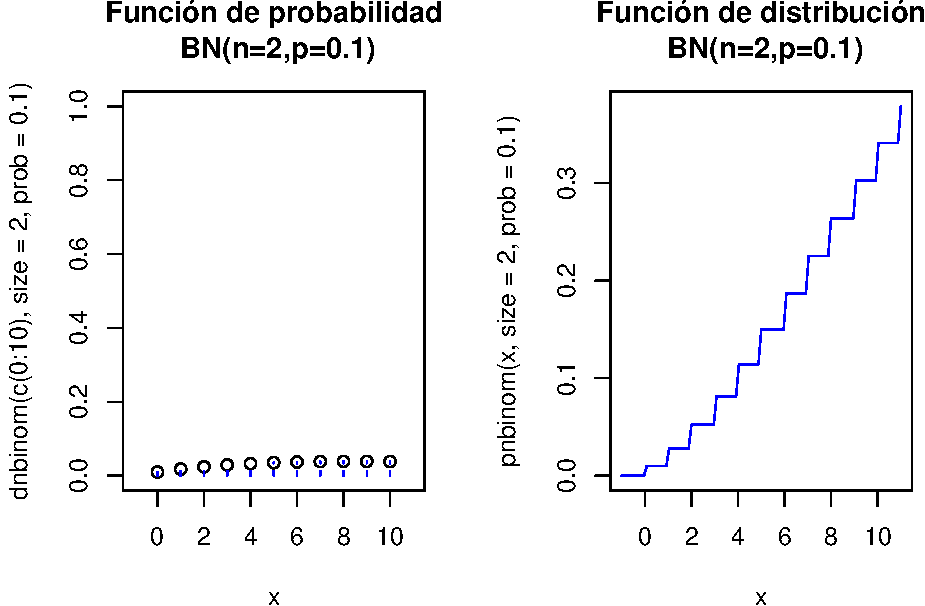
\includegraphics{curso-probabilidad-udemy_files/figure-latex/unnamed-chunk-46-1} \end{center}

\hypertarget{gruxe1ficas-interactivas-binomial-negativa}{%
\subsection{Gráficas interactivas binomial negativa}\label{gruxe1ficas-interactivas-binomial-negativa}}

Para ejecutar el siguiente gráfico interactivo, solamente tienes que cargar el paquete \texttt{shiny} en tu ordenador y luego copiar/pegar las siguientes instrucciones. De este modo podrás observar los cambios en las distribuciones variando los parámetros.

\begin{Shaded}
\begin{Highlighting}[]
\KeywordTok{fluidPage}\NormalTok{(}
\KeywordTok{fluidRow}\NormalTok{(}
  \KeywordTok{column}\NormalTok{(}\DecValTok{6}\NormalTok{,}
         \KeywordTok{sliderInput}\NormalTok{(}\StringTok{"n_nbinom"}\NormalTok{, }\DataTypeTok{label =} \StringTok{"Número de éxitos n:"}\NormalTok{,}
              \DataTypeTok{min =} \DecValTok{1}\NormalTok{, }\DataTypeTok{max =} \DecValTok{50}\NormalTok{, }\DataTypeTok{value =}\DecValTok{20}\NormalTok{ , }\DataTypeTok{step =} \DecValTok{1}\NormalTok{)),}
  \KeywordTok{column}\NormalTok{(}\DecValTok{6}\NormalTok{,}
          \KeywordTok{sliderInput}\NormalTok{(}\StringTok{"p_nbinom"}\NormalTok{, }\DataTypeTok{label =} \StringTok{"Probabilidad de un éxito p:"}\NormalTok{,}
                     \DataTypeTok{min =} \FloatTok{0.01}\NormalTok{, }\DataTypeTok{max =} \FloatTok{0.99}\NormalTok{, }\DataTypeTok{value =} \FloatTok{0.8}\NormalTok{, }\DataTypeTok{step =} \FloatTok{0.01}\NormalTok{)}
\NormalTok{         )}
\NormalTok{  )}
\NormalTok{)}

\KeywordTok{renderPlot}\NormalTok{(\{}
\NormalTok{  n=input}\OperatorTok{$}\NormalTok{n_nbinom}
\NormalTok{  pr=input}\OperatorTok{$}\NormalTok{p_nbinom}
  
  \KeywordTok{par}\NormalTok{(}\DataTypeTok{mfrow=}\KeywordTok{c}\NormalTok{(}\DecValTok{1}\NormalTok{,}\DecValTok{2}\NormalTok{))}
\NormalTok{  aux=}\KeywordTok{rep}\NormalTok{(}\DecValTok{0}\NormalTok{,(n}\OperatorTok{+}\DecValTok{1}\NormalTok{)}\OperatorTok{*}\DecValTok{2}\NormalTok{)}
\NormalTok{  aux[}\KeywordTok{seq}\NormalTok{(}\DecValTok{2}\NormalTok{,(n}\OperatorTok{+}\DecValTok{1}\NormalTok{)}\OperatorTok{*}\DecValTok{2}\NormalTok{,}\DecValTok{2}\NormalTok{)]=}\KeywordTok{dnbinom}\NormalTok{(}\KeywordTok{c}\NormalTok{(}\DecValTok{0}\OperatorTok{:}\NormalTok{n),}\DataTypeTok{size=}\NormalTok{n,}\DataTypeTok{prob=}\NormalTok{pr)}
  \KeywordTok{plot}\NormalTok{(}\DataTypeTok{x=}\KeywordTok{c}\NormalTok{(}\DecValTok{0}\OperatorTok{:}\NormalTok{n),}\DataTypeTok{y=}\KeywordTok{dnbinom}\NormalTok{(}\KeywordTok{c}\NormalTok{(}\DecValTok{0}\OperatorTok{:}\NormalTok{n),}\DataTypeTok{size=}\NormalTok{n,}\DataTypeTok{prob=}\NormalTok{pr),}
       \DataTypeTok{ylim=}\KeywordTok{c}\NormalTok{(}\DecValTok{0}\NormalTok{,}\DecValTok{1}\NormalTok{),}\DataTypeTok{xlim=}\KeywordTok{c}\NormalTok{(}\OperatorTok{-}\DecValTok{1}\NormalTok{,n}\OperatorTok{+}\DecValTok{1}\NormalTok{),}\DataTypeTok{xlab=}\StringTok{"x"}\NormalTok{,}
       \DataTypeTok{main=}\KeywordTok{paste0}\NormalTok{(}\KeywordTok{c}\NormalTok{(}\StringTok{"Función de probabilidad}\CharTok{\textbackslash{}n}\StringTok{ BN(n="}\NormalTok{,n,}\StringTok{",p="}\NormalTok{,pr,}\StringTok{")"}\NormalTok{),}\DataTypeTok{collapse =} \StringTok{""}\NormalTok{))}
  \KeywordTok{lines}\NormalTok{(}\DataTypeTok{x=}\KeywordTok{rep}\NormalTok{(}\DecValTok{0}\OperatorTok{:}\NormalTok{n,}\DataTypeTok{each=}\DecValTok{2}\NormalTok{),}\DataTypeTok{y=}\NormalTok{aux, }\DataTypeTok{type =} \StringTok{"h"}\NormalTok{, }\DataTypeTok{lty =} \DecValTok{2}\NormalTok{,}\DataTypeTok{col=}\StringTok{"blue"}\NormalTok{)}
  \KeywordTok{curve}\NormalTok{(}\KeywordTok{pnbinom}\NormalTok{(x,}\DataTypeTok{size=}\NormalTok{n,}\DataTypeTok{p=}\NormalTok{pr),}
        \DataTypeTok{xlim=}\KeywordTok{c}\NormalTok{(}\OperatorTok{-}\DecValTok{1}\NormalTok{,n}\OperatorTok{+}\DecValTok{1}\NormalTok{),}\DataTypeTok{col=}\StringTok{"blue"}\NormalTok{,}
        \DataTypeTok{main=}\KeywordTok{paste0}\NormalTok{(}\KeywordTok{c}\NormalTok{(}\StringTok{"Función de distribución\textbackslash{}n BN(n="}\NormalTok{,n,}\StringTok{",p="}\NormalTok{,pr,}\StringTok{")"}\NormalTok{),}
                    \DataTypeTok{collapse =} \StringTok{""}\NormalTok{))}
  \KeywordTok{par}\NormalTok{(}\DataTypeTok{mfrow=}\KeywordTok{c}\NormalTok{(}\DecValTok{1}\NormalTok{,}\DecValTok{1}\NormalTok{))}
\NormalTok{\})}
\end{Highlighting}
\end{Shaded}

\href{https://joanby.shinyapps.io/DistribucionesNotables/}{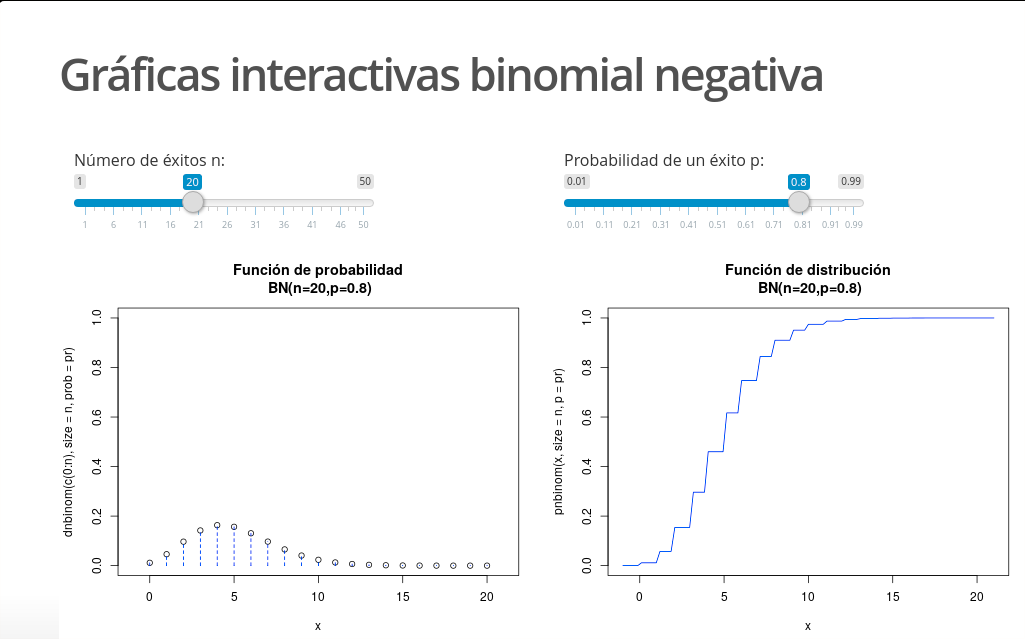
\includegraphics{Images/noshinyImages/interactiva_binomial_negativa1.png}}

\hypertarget{gruxe1ficos-de-la-binomial-negativa-con-python}{%
\subsection{Gráficos de la binomial negativa con python}\label{gruxe1ficos-de-la-binomial-negativa-con-python}}

\textbf{Ejercicio}

Buscad en los manuales de python cómo se dibuja la función de probabilidad y de distribución de una binomial.
negativa

Necesitamos de nuevo más librerías

\begin{Shaded}
\begin{Highlighting}[]
\ImportTok{import}\NormalTok{ numpy }\ImportTok{as}\NormalTok{ np}
\ImportTok{from}\NormalTok{ scipy.stats }\ImportTok{import}\NormalTok{ nbinom}
\ImportTok{import}\NormalTok{ matplotlib.pyplot }\ImportTok{as}\NormalTok{ plt}
\end{Highlighting}
\end{Shaded}

\hypertarget{gruxe1ficos-de-la-binomial-negativa-con-python-1}{%
\subsection{Gráficos de la binomial negativa con python}\label{gruxe1ficos-de-la-binomial-negativa-con-python-1}}

\begin{Shaded}
\begin{Highlighting}[]
\NormalTok{n, p }\OperatorTok{=} \DecValTok{10}\NormalTok{, }\FloatTok{0.25}
\NormalTok{x }\OperatorTok{=}\NormalTok{ np.arange(}\DecValTok{0}\NormalTok{,nbinom.ppf(}\FloatTok{0.99}\NormalTok{, n, p))}
\NormalTok{fig }\OperatorTok{=}\NormalTok{plt.figure(figsize}\OperatorTok{=}\NormalTok{(}\DecValTok{5}\NormalTok{, }\FloatTok{2.7}\NormalTok{))}
\NormalTok{ax }\OperatorTok{=}\NormalTok{ fig.add_subplot(}\DecValTok{1}\NormalTok{,}\DecValTok{2}\NormalTok{,}\DecValTok{1}\NormalTok{)}
\NormalTok{ax.plot(x, nbinom.pmf(x, n, p), }\StringTok{'bo'}\NormalTok{, ms}\OperatorTok{=}\DecValTok{5}\NormalTok{, label}\OperatorTok{=}\StringTok{'nbinom pmf'}\NormalTok{)}
\NormalTok{ax.vlines(x, }\DecValTok{0}\NormalTok{, nbinom.pmf(x, n, p), colors}\OperatorTok{=}\StringTok{'b'}\NormalTok{, lw}\OperatorTok{=}\DecValTok{2}\NormalTok{, alpha}\OperatorTok{=}\FloatTok{0.5}\NormalTok{)}
\ControlFlowTok{for}\NormalTok{ tick }\KeywordTok{in}\NormalTok{ ax.xaxis.get_major_ticks():}
\NormalTok{  tick.label.set_fontsize(}\DecValTok{5}\NormalTok{)}
\ControlFlowTok{for}\NormalTok{ tick }\KeywordTok{in}\NormalTok{ ax.yaxis.get_major_ticks():}
\NormalTok{  tick.label.set_fontsize(}\DecValTok{5}\NormalTok{) }
\NormalTok{ax }\OperatorTok{=}\NormalTok{ fig.add_subplot(}\DecValTok{1}\NormalTok{,}\DecValTok{2}\NormalTok{,}\DecValTok{2}\NormalTok{)}
\NormalTok{ax.plot(x, nbinom.cdf(x, n, p), }\StringTok{'bo'}\NormalTok{, ms}\OperatorTok{=}\DecValTok{5}\NormalTok{, label}\OperatorTok{=}\StringTok{'nbinom pmf'}\NormalTok{)}
\NormalTok{ax.vlines(x, }\DecValTok{0}\NormalTok{, nbinom.cdf(x, n, p), colors}\OperatorTok{=}\StringTok{'b'}\NormalTok{, lw}\OperatorTok{=}\DecValTok{2}\NormalTok{, alpha}\OperatorTok{=}\FloatTok{0.5}\NormalTok{)}
\ControlFlowTok{for}\NormalTok{ tick }\KeywordTok{in}\NormalTok{ ax.xaxis.get_major_ticks():}
\NormalTok{  tick.label.set_fontsize(}\DecValTok{5}\NormalTok{)}
\ControlFlowTok{for}\NormalTok{ tick }\KeywordTok{in}\NormalTok{ ax.yaxis.get_major_ticks():}
\NormalTok{  tick.label.set_fontsize(}\DecValTok{5}\NormalTok{)}
\NormalTok{fig.suptitle(}\StringTok{'Distribucion Binomial Negativa'}\NormalTok{)}
\NormalTok{plt.show()}
\end{Highlighting}
\end{Shaded}

\hypertarget{gruxe1ficos-de-la-binomial-negativa-con-python-2}{%
\subsection{Gráficos de la binomial negativa con python}\label{gruxe1ficos-de-la-binomial-negativa-con-python-2}}

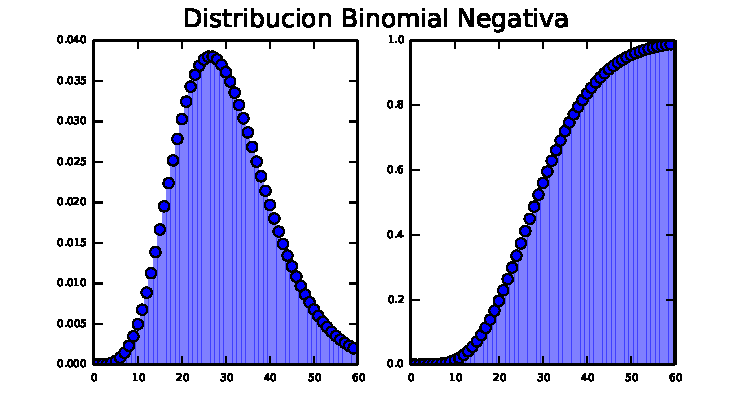
\includegraphics{curso-probabilidad-udemy_files/figure-latex/negativa_py_show-1.pdf}

\hypertarget{ejercicio-acceso-aleatorio-a-un-sistema-con-triple-clave.}{%
\subsection{Ejercicio: Acceso aleatorio a un sistema con triple clave.}\label{ejercicio-acceso-aleatorio-a-un-sistema-con-triple-clave.}}

\textbf{Sistema con tres claves de acceso}

Supongamos que tenemos un sistema informático tiene un programa de seguridad que genera accesos con claves de 3 dígitos \(000,001,\ldots 999\). En total 1000 posibilidades.

Como una clave de tres dígitos es fácil de romper proponemos poner tres claves consecutivas de acceso al sistema cada una de 3 dígitos.

Para acceder al sistema hay que dar las tres claves de forma consecutiva y por orden.

Es decir hasta que no averiguamos la primera clave no pasamos a la segunda clave.

Supongamos que cada vez que ponemos los dos dígitos olvidamos el resultado y seguimos poniendo dígitos al azar hasta adivinar la contraseña.

Así hasta conseguir entrar en el sistema.

Sea \(X\) la v.a que nos da el número de fallos antes de entrar en el sistema.

\hypertarget{ejercicio-acceso-aleatorio-a-un-sistema-con-triple-clave.-1}{%
\subsection{Ejercicio acceso aleatorio a un sistema con triple clave.}\label{ejercicio-acceso-aleatorio-a-un-sistema-con-triple-clave.-1}}

Estamos interesados en modelar este problema. La preguntas son:

\begin{enumerate}
\def\labelenumi{\arabic{enumi}.}
\tightlist
\item
  ¿Cuál es la distribución de probabilidad de \(X\) la v.a que nos da el número de fallos antes de acceder al sistema.
\item
  ¿Cuál es la función de probabilidad y de distribución del \(X\)
\item
  ¿Cuál es la probabilidad de fallar 150 veces antes de acceder en el sistema?
\item
  ¿Cuál es la probabilidad de fallar más de 150 veces antes de entrar en el sistema?
\item
  ¿Cuál es el número esperado de fallos antes de acceder al sistema? ¿Y su desviación típica?
\end{enumerate}

\hypertarget{ejemplo-bnrp}{%
\subsection{\texorpdfstring{Ejemplo \(BN(r,p)\)}{Ejemplo BN(r,p)}}\label{ejemplo-bnrp}}

\textbf{Solución 1.} ¿Cuál es la distribución de probabilidad de \(X\) la v.a que nos da el número de fallos antes de acceder al sistema.

Bajo estados condiciones tenemos que la probabilidad de ``éxito'' de cada intento es \(p=\frac{1}{1000}=0.001\). Y como cada vez \emph{olvidamos} en los dígitos cada intento será independiente del anterior.

Así que la variable \(X\) cuenta el número de fracasos independientes hasta conseguir 3 éxitos en un experimento \(Ber(p=0.001)\) por lo tanto \(X\) sigue un distribución \(BN(n=3,p=0.001).\)

\hypertarget{ejemplo-bnrp-1}{%
\subsection{\texorpdfstring{Ejemplo \(BN(r,p)\)}{Ejemplo BN(r,p)}}\label{ejemplo-bnrp-1}}

\textbf{Solución 2.} ¿Cuál es la función de probabilidad y de distribución del \(X\)

En general la función de probabilidad de una \(BN(n,p)\) es

\[
P_X(X=x)=P(X=x)=
\left\{
\begin{array}{cc} 
{x+n-1\choose n-1} \cdot (1-p)^{x}\cdot p^n & \mbox{si }  x=0,1,\ldots \\ 0 & \mbox{en otro caso.}\end{array}\right.
\]
En particular la función de probabilidad de una \(BN(n=3,p=0.001)\) es

\[
P_X(X=x)=P(X=x)=
\left\{
\begin{array}{cc} 
{x+2\choose 2} \cdot 0.999^{x}\cdot 0.001^3 & \mbox{si }  x=0,1,2,\ldots \\ 0 & \mbox{en otro caso.}\end{array}\right.
\]

\hypertarget{soluciuxf3n-ejemplo-bnn3p0.001}{%
\subsection{\texorpdfstring{Solución ejemplo \(BN(n=3,p=0.001)\)}{Solución ejemplo BN(n=3,p=0.001)}}\label{soluciuxf3n-ejemplo-bnn3p0.001}}

\textbf{Solución 3.} ¿Cuál es la probabilidad de fallar 150 veces antes de acceder en el sistema?

Nos piden

\[
P(X=150)= {152\choose 2} \cdot 0.999^{150}\cdot 0.001^3
\]

Lo calcularemos operando con R

\begin{Shaded}
\begin{Highlighting}[]
\KeywordTok{choose}\NormalTok{(}\DecValTok{152}\NormalTok{,}\DecValTok{2}\NormalTok{)}\OperatorTok{*}\FloatTok{0.999}\OperatorTok{^}\DecValTok{150}\OperatorTok{*}\FloatTok{0.001}\OperatorTok{^}\DecValTok{3}
\end{Highlighting}
\end{Shaded}

\begin{verbatim}
## [1] 9.876743e-06
\end{verbatim}

con la función de R

\begin{Shaded}
\begin{Highlighting}[]
\KeywordTok{dnbinom}\NormalTok{(}\DecValTok{150}\NormalTok{,}\DataTypeTok{size=}\DecValTok{3}\NormalTok{,}\DataTypeTok{p=}\FloatTok{0.001}\NormalTok{)}
\end{Highlighting}
\end{Shaded}

\begin{verbatim}
## [1] 9.876743e-06
\end{verbatim}

\hypertarget{soluciuxf3n-ejemplo-bnn3p0.001-1}{%
\subsection{\texorpdfstring{Solución ejemplo \(BN(n=3,p=0.001)\)}{Solución ejemplo BN(n=3,p=0.001)}}\label{soluciuxf3n-ejemplo-bnn3p0.001-1}}

\textbf{Solución 3.} ¿Cuál es la probabilidad de fallar 150 veces antes de acceder en el sistema?

Nos piden

\[
P(X=150)= {152\choose 2} \cdot 0.999^{150}\cdot 0.001^3
\]

Pero también lo podemos hacer con python

\begin{Shaded}
\begin{Highlighting}[]
\ImportTok{from}\NormalTok{  scipy.special }\ImportTok{import}\NormalTok{ binom}
\NormalTok{binom(}\DecValTok{152}\NormalTok{,}\DecValTok{2}\NormalTok{)}\OperatorTok{*}\FloatTok{0.999}\OperatorTok{**}\DecValTok{150}\OperatorTok{*}\FloatTok{0.001}\OperatorTok{**}\DecValTok{3}
\end{Highlighting}
\end{Shaded}

\begin{verbatim}
## 9.8767434596705257e-06
\end{verbatim}

\begin{Shaded}
\begin{Highlighting}[]
\NormalTok{nbinom.pmf(}\DecValTok{150}\NormalTok{,n}\OperatorTok{=}\DecValTok{3}\NormalTok{,p}\OperatorTok{=}\FloatTok{0.001}\NormalTok{)}
\end{Highlighting}
\end{Shaded}

\begin{verbatim}
## 9.8767434596702174e-06
\end{verbatim}

\hypertarget{soluciuxf3n-ejemplo-bnnp}{%
\subsection{\texorpdfstring{Solución ejemplo \(BN(n,p)\)}{Solución ejemplo BN(n,p)}}\label{soluciuxf3n-ejemplo-bnnp}}

\textbf{Solución 4.} ¿Cuál es la probabilidad de fallar más de 150 veces antes de entrar en el sistema?

\[P(X>150)=1-P(X\leq 150)\]

Calculemos \(P(X\leq 150)\)

\[
\begin{eqnarray*}
P(X\leq 150) &=& P(X=0)+P(X=1)+P(X=2)+\ldots+P(X=150)= \sum_{k=0}^{150} {k+3-1\choose 3-1} \cdot (0.999)^{k}\cdot 0.001^3\\
&=& \ldots = \ensuremath{5.2320035\times 10^{-4}}
\end{eqnarray*}
\]

\begin{Shaded}
\begin{Highlighting}[]
\KeywordTok{pnbinom}\NormalTok{(}\DecValTok{150}\NormalTok{,}\DecValTok{3}\NormalTok{,}\FloatTok{0.001}\NormalTok{)}
\end{Highlighting}
\end{Shaded}

\begin{verbatim}
## [1] 0.0005232003
\end{verbatim}

\begin{Shaded}
\begin{Highlighting}[]
\NormalTok{nbinom.cdf(}\DecValTok{150}\NormalTok{,n}\OperatorTok{=}\DecValTok{3}\NormalTok{,p}\OperatorTok{=}\FloatTok{0.001}\NormalTok{)}
\end{Highlighting}
\end{Shaded}

\begin{verbatim}
## 0.00052320034908240592
\end{verbatim}

\hypertarget{soluciuxf3n-ejemplo-bnnp-1}{%
\subsection{\texorpdfstring{Solución ejemplo \(BN(n,p)\)}{Solución ejemplo BN(n,p)}}\label{soluciuxf3n-ejemplo-bnnp-1}}

\textbf{Solución 5.} ¿Cuál es el número esperado de fallos antes de acceder al sistema? ¿Y su desviación típica?

\[E(X)=n\cdot \frac{1-p}{p}=3\cdot \frac{1- 0.001}{0.001}=2997.\]
\[Var(X)=n\cdot \frac{1-p}{p^2}=3\cdot \frac{1- 0.001^2}{0.001^2}=\ensuremath{2.997\times 10^{6}}.\]

Con python

\begin{Shaded}
\begin{Highlighting}[]
\NormalTok{params }\OperatorTok{=}\NormalTok{ nbinom.stats(n}\OperatorTok{=}\DecValTok{3}\NormalTok{,p}\OperatorTok{=}\FloatTok{0.001}\NormalTok{,moments}\OperatorTok{=}\StringTok{'mv'}\NormalTok{)}
\BuiltInTok{print}\NormalTok{(}\StringTok{"E(X) = }\SpecialCharTok{\{m\}}\StringTok{"}\NormalTok{.}\BuiltInTok{format}\NormalTok{(m}\OperatorTok{=}\NormalTok{params[}\DecValTok{0}\NormalTok{]))}
\end{Highlighting}
\end{Shaded}

\begin{verbatim}
## E(X) = 2997.0
\end{verbatim}

\begin{Shaded}
\begin{Highlighting}[]
\BuiltInTok{print}\NormalTok{(}\StringTok{"Var(X) = }\SpecialCharTok{\{v\}}\StringTok{"}\NormalTok{.}\BuiltInTok{format}\NormalTok{(v}\OperatorTok{=}\NormalTok{params[}\DecValTok{1}\NormalTok{]))}
\end{Highlighting}
\end{Shaded}

\begin{verbatim}
## Var(X) = 2997000.0
\end{verbatim}

\hypertarget{tres-claves-de-tres-duxedgitos-o-una-de-9-duxedgitos}{%
\subsection{¿Tres claves de tres dígitos o una de 9 dígitos?}\label{tres-claves-de-tres-duxedgitos-o-una-de-9-duxedgitos}}

\textbf{Ejercicio}

Supongamos que ponemos una sola clave de 9 dígitos. Estudiemos en este caso la variable aleatoria que da el número de fallos antes de entrar en el sistema y comparemos los resultados.

Si seguimos suponiendo que cada vez ponemos la contraseña al azar pero esta vez con una clave de 9 dígitos. La probabilidad de éxito será ahora \(p=\frac{1}{10^{9}}\).

Si llamamos \(X_9\) a la variable aleatoria que nos da el número de fallos antes de entra en el sistema seguirá una distribución \(Ge(p=\frac{1}{10^9}=0.000000001)\).

\hypertarget{quuxe9-da-muxe1s-seguridad-tres-claves-de-tres-duxedgitos-o-una-de-9-duxedgitos}{%
\subsection{Qué da más seguridad ¿tres claves de tres dígitos o una de 9 dígitos?}\label{quuxe9-da-muxe1s-seguridad-tres-claves-de-tres-duxedgitos-o-una-de-9-duxedgitos}}

Su valor esperado es

\[
E(X_9)=\frac{1-p}{p}=\frac{1-0.000000001}{0.000000001}=\ensuremath{10\times 10^{8}}.
\]

\(1000 000 000\) son 1000 millones de fallos esperados hasta abrir la puerta.

Recordemos que con tres contraseñas de 3 dígitos el valor esperado de fallos es

\[3\cdot \frac{1-0.001}{0.001}=2997.\]

Por lo tanto es mejor una clave larga de 9 dígitos que tres cortas si escribimos las contraseñas al azar.

\hypertarget{distribuciuxf3n-poisson}{%
\section{Distribución Poisson}\label{distribuciuxf3n-poisson}}

Diremos que una v.a. discreta \(X\) con \(X(\Omega)=\mathbf{N}\) tiene distribución de Poisson con parámetro \(\lambda>0\), y lo denotaremos por \(Po(\lambda)\) si su función de probabilidad es:

\[
P_{X}(x)=P(X=x)=
\left\{\begin{array}{ll}
\frac{\lambda^x}{x!} e^{-\lambda}& \mbox{ si } x=0,1,\ldots\\
0 & \mbox{en otro caso}\end{array}\right..
\]

Recordemos que el desarrollo en serie de Taylor de la exponencial es

\[
e^{\lambda}=\sum_{x=0}^{+\infty} \frac{\lambda^x}{x!}.
\]

Teniendo en cuenta esto es fácil comprobar que todos los valores de la función de probabilidad suman 1.

Además recordemos que dado \(x\in\mathbb{R}-\{0\}\) se tiene que

\[
\lim_{n\to\infty} \left(1+\frac{x}{n}\right)^n=e^x.
\]

\hypertarget{distribuciuxf3n-poisson-1}{%
\subsection{Distribución Poisson}\label{distribuciuxf3n-poisson-1}}

Así, por ejemplo, se tiene que

\[
\lim_{n\to\infty} \left(1-\frac{\lambda}{n}\right)^n=\lim_{n\to\infty} \left(1+\frac{-\lambda}{n}\right)^n=e^{-\lambda}.
\]

\hypertarget{la-distribuciuxf3n-poisson-como-luxedmite-de-una-binomial.}{%
\subsection{La distribución Poisson como ``límite'' de una binomial.}\label{la-distribuciuxf3n-poisson-como-luxedmite-de-una-binomial.}}

La distribución Poisson (\href{https://es.wikipedia.org/wiki/Sim\%C3\%A9on_Denis_Poisson}{Siméon Denis Poisson}) aparece en el conteo de determinados eventos que se producen en un intervalo de tiempo o en el espacio.

Supongamos que nuestra variable de interés es \(X\)= número de eventos en el intervalo de tiempo \((0,t]\).

Como por ejemplo el número de llamadas a un \emph{call center} en una hora y que sabemos que se cumplen las siguientes condiciones:

\hypertarget{la-distribuciuxf3n-poisson-como-luxedmite-de-una-binomial.-1}{%
\subsection{La distribución Poisson como ``límite'' de una binomial.}\label{la-distribuciuxf3n-poisson-como-luxedmite-de-una-binomial.-1}}

\begin{enumerate}
\def\labelenumi{\arabic{enumi}.}
\tightlist
\item
  El número promedio de eventos en el intervalo \((0,t]\) es
  \(\lambda>0\).
\item
  Es posible dividir el intervalo de tiempo en un
  gran número de subintervalos (denotemos por \(n\) al número de intervalos) de forma que:

  \begin{itemize}
  \tightlist
  \item
    La probabilidad de que se produzcan dos o más eventos en un subintervalo es despreciable.
  \item
    El número de ocurrencias de eventos en un intervalo es independiente del número de ocurrencias en otro intervalo.
  \item
    La probabilidad de que un evento ocurra en un subintervalo es \(p_n\cdot n=\lambda\) o lo que es lo mismo \(p_n=\frac{\lambda}{n}\)·
  \end{itemize}
\end{enumerate}

\hypertarget{la-distribuciuxf3n-poisson-como-luxedmite-de-una-binomial.-2}{%
\subsection{La distribución Poisson como ``límite'' de una binomial.}\label{la-distribuciuxf3n-poisson-como-luxedmite-de-una-binomial.-2}}

Bajo estas condiciones podemos considerar que el número de eventos en el intervalo \((0,t]\) será el número de ``éxitos'' en \(n\) repeticiones independientes de un proceso Bernoulli de parámetro \(p_n\)

Entonces si \(n\to\infty\) y \(p_n\cdot n\) se mantiene igual a \(\lambda\) resulta que la función de probabilidad de \(X\) se puede poner como

\hypertarget{la-distribuciuxf3n-poisson-como-luxedmite-de-una-binomial.-3}{%
\subsection{La distribución Poisson como ``límite'' de una binomial.}\label{la-distribuciuxf3n-poisson-como-luxedmite-de-una-binomial.-3}}

\[
\begin{eqnarray*}
P(X_n=k)&=&\left(\begin{array}{c} n\\ k\end{array}\right) \cdot p_n^k\cdot  (1-p_n)^{n-k}
\\
&=& {n\choose k}\cdot \left(\frac{\lambda}{n}\right)^{k}\cdot \left(1-\frac{\lambda}{n}\right)^{n-k}\\
&=&
\frac{\lambda^k}{k!}\cdot\frac{n!}{(n-k)!\cdot n^k}\cdot
\left(1-\frac{\lambda}{n}\right)^{n}\cdot \left(1-\frac{\lambda}{n}\right)^{-k}=\ldots
\end{eqnarray*}
\]

\hypertarget{la-distribuciuxf3n-poisson-como-luxedmite-de-una-binomial.-4}{%
\subsection{La distribución Poisson como ``límite'' de una binomial.}\label{la-distribuciuxf3n-poisson-como-luxedmite-de-una-binomial.-4}}

Estamos interesados en calcular

\[
\displaystyle\lim_{n\to \infty} P(X_n=k) = \lim_{n\to \infty} \frac{\lambda^k}{k!}\cdot\frac{n!}{(n-k)!\cdot n^k} \cdot
\left(1-\frac{\lambda}{n}\right)^{n}\cdot \left(1-\frac{\lambda}{n}\right)^{-k}.
\]

Calculemos el límite de algunos de los factores de la expresión

\[
\displaystyle\lim_{n\to \infty}\frac{n!}{(n-k)!\cdot n^k}= \lim_{n\to \infty}\frac{n\cdot (n-1)\cdots (n-k-1)}{n^k}
=\lim_{n\to \infty}\frac{n^{k}+\cdots}{n^k}=1.
\]

\hypertarget{la-distribuciuxf3n-poisson-como-luxedmite-de-una-binomial.-5}{%
\subsection{La distribución Poisson como ``límite'' de una binomial.}\label{la-distribuciuxf3n-poisson-como-luxedmite-de-una-binomial.-5}}

\[
\lim_{n\to \infty} \left(1-\frac{\lambda}{n}\right)^{n}=e^{-\lambda}
\]

Y también teniendo en cuanta que \(k\) es constante.

\[
\lim_{n\to \infty} \left(1-\frac{\lambda}{n}\right)^{-k}=\lim_{n\to \infty} 1^{-k}=\lim_{n\to \infty}  1=1.
\]

\hypertarget{la-distribuciuxf3n-poisson-como-luxedmite-de-una-binomial.-6}{%
\subsection{La distribución Poisson como ``límite'' de una binomial.}\label{la-distribuciuxf3n-poisson-como-luxedmite-de-una-binomial.-6}}

Para acabar

\[
\displaystyle\lim_{n\to\infty} P(X_n=k)=
\lim_{n\to\infty} \left(\begin{array}{c} n\\ k\end{array}\right)
\cdot p_n^k \cdot (1-p_n)^{n-k}= \frac{\lambda^k}{k!}\cdot 1 \cdot e^{-\lambda}\cdot 1=\frac{\lambda^k}{k!}\cdot e^{-\lambda}.
\]

Lo que confirma que límite de una serie de variables
\(B(n,p_n=\frac{\lambda}{n})\) sigue una ley \(Po(\lambda)\).

\hypertarget{procesos-de-poisson}{%
\subsection{Procesos de Poisson}\label{procesos-de-poisson}}

Lo interesante de las variables Poisson es que podemos modificar (si el modelo lo permite) el intervalo de tiempo \((0,t]\) en el que contamos los eventos.

Claro que esto no tiene que poder ser así.

Pero en general si la variable es poisson en \((0,t]\) también lo será en cualquier subintervalo \((0,t']\) para todo \(t'\) tal que \(0<t'<t\).

Así que podremos definir una serie de variables \(X_t\) de distribución \(Po(\lambda\cdot t)\).

\hypertarget{procesos-de-poisson-1}{%
\subsection{Procesos de Poisson}\label{procesos-de-poisson-1}}

 Definición procesos de Poisson

Consideremos un experimento \emph{Poisson} con \(\lambda\) igual
al promedio de eventos en una unidad de tiempo (u.t.).

Si \(t\) es una cantidad de tiempo en u.t., la v.a. \(X_{t}\)=numero de eventos en el intervalo \((0,t]\) es una \(Po(\lambda\cdot t)\).

El conjunto de variables \(\{X_t\}_{t>0}\) recibe el nombre de \textbf{proceso de Poisson}.

\hypertarget{resumen-distribuciuxf3n-poisson-xequiv-polambda}{%
\subsection{\texorpdfstring{Resumen distribución Poisson \(X\equiv Po(\lambda)\)}{Resumen distribución Poisson X\textbackslash{}equiv Po(\textbackslash{}lambda)}}\label{resumen-distribuciuxf3n-poisson-xequiv-polambda}}

\begin{longtable}[]{@{}rl@{}}
\toprule
\begin{minipage}[b]{0.47\columnwidth}\raggedleft
\(X\) Poisson\strut
\end{minipage} & \begin{minipage}[b]{0.47\columnwidth}\raggedright
\(\lambda\)\strut
\end{minipage}\tabularnewline
\midrule
\endhead
\begin{minipage}[t]{0.47\columnwidth}\raggedleft
\(D_X=\)\strut
\end{minipage} & \begin{minipage}[t]{0.47\columnwidth}\raggedright
\(\{0,1,\ldots \}\)\strut
\end{minipage}\tabularnewline
\begin{minipage}[t]{0.47\columnwidth}\raggedleft
\(P_X(x)=P(X=x)=\)\strut
\end{minipage} & \begin{minipage}[t]{0.47\columnwidth}\raggedright
\(\left\{\begin{array}{ll} \frac{\lambda^x}{x!}e^{-\lambda} & \mbox{ si } x=0,1,\ldots\\ 0 & \mbox{ en otro caso.}\end{array}\right.\)\strut
\end{minipage}\tabularnewline
\begin{minipage}[t]{0.47\columnwidth}\raggedleft
\(F_X(x)=P(X\leq X)=\)\strut
\end{minipage} & \begin{minipage}[t]{0.47\columnwidth}\raggedright
\(\begin{array}{l}\left\{\begin{array}{ll} 0 & \mbox{si } x<0\\\displaystyle\sum_{i=0}^{k} P(X=i)= \displaystyle\sum_{i=0}^{k} \frac{\lambda^i}{i!}\cdot e^{-\lambda} & \mbox{si }\left\{\begin{array}{l}k\leq x< k+1\\k=0,1,2,\ldots\end{array}\right.\end{array}\right. \\\mbox{Calcular la suma o utilizar funciones de R o python.} \end{array}\)\strut
\end{minipage}\tabularnewline
\begin{minipage}[t]{0.47\columnwidth}\raggedleft
\(E(X)=\lambda\)\strut
\end{minipage} & \begin{minipage}[t]{0.47\columnwidth}\raggedright
\(Var(X)=\lambda\)\strut
\end{minipage}\tabularnewline
\bottomrule
\end{longtable}

\hypertarget{resumen-proceso-poisson-x_tequiv-polambdacdot-t}{%
\subsection{\texorpdfstring{Resumen proceso Poisson \(X_t\equiv Po(\lambda\cdot t)\)}{Resumen proceso Poisson X\_t\textbackslash{}equiv Po(\textbackslash{}lambda\textbackslash{}cdot t)}}\label{resumen-proceso-poisson-x_tequiv-polambdacdot-t}}

\begin{longtable}[]{@{}rl@{}}
\toprule
\begin{minipage}[b]{0.47\columnwidth}\raggedleft
\(X_t\) \(Po(\lambda\cdot t)\)\strut
\end{minipage} & \begin{minipage}[b]{0.47\columnwidth}\raggedright
\(\lambda\) promedio por u.t.\strut
\end{minipage}\tabularnewline
\midrule
\endhead
\begin{minipage}[t]{0.47\columnwidth}\raggedleft
\(D_X=\)\strut
\end{minipage} & \begin{minipage}[t]{0.47\columnwidth}\raggedright
\(\{0,1,\ldots \}\)\strut
\end{minipage}\tabularnewline
\begin{minipage}[t]{0.47\columnwidth}\raggedleft
\(P_X(x)=P(X=x)=\)\strut
\end{minipage} & \begin{minipage}[t]{0.47\columnwidth}\raggedright
\(\left\{\begin{array}{ll} \frac{(\lambda\cdot t)^x}{x!}e^{-\lambda\cdot t} & \mbox{ si } x=0,1,\ldots\\ 0 & \mbox{ en otro caso.}\end{array}\right.\)\strut
\end{minipage}\tabularnewline
\begin{minipage}[t]{0.47\columnwidth}\raggedleft
\(F_X(x)=P(X\leq X)=\)\strut
\end{minipage} & \begin{minipage}[t]{0.47\columnwidth}\raggedright
\(\begin{array}{l}\left\{\begin{array}{ll} 0 & \mbox{si } x<0\\\displaystyle\sum_{i=0}^{k} P(X=i)= \displaystyle\sum_{i=0}^{k} \frac{(\lambda\cdot t)^i}{i!}\cdot e^{-\lambda\cdot t} & \mbox{si }\left\{\begin{array}{l}k\leq x< k+1\\k=0,1,2,\ldots\end{array}\right.\end{array}\right. \\\mbox{Calcular la suma o utilizar funciones de R o python.} \end{array}\)\strut
\end{minipage}\tabularnewline
\begin{minipage}[t]{0.47\columnwidth}\raggedleft
\(E(X)=\lambda\cdot t\)\strut
\end{minipage} & \begin{minipage}[t]{0.47\columnwidth}\raggedright
\(Var(X)=\lambda\cdot t\)\strut
\end{minipage}\tabularnewline
\bottomrule
\end{longtable}

\hypertarget{aproximaciuxf3n-de-la-distribuciuxf3n-binomial-por-la-poisson}{%
\subsection{Aproximación de la distribución binomial por la Poisson}\label{aproximaciuxf3n-de-la-distribuciuxf3n-binomial-por-la-poisson}}

Bajo el punto de vista anterior y si \(p\) es pequeño y \(n\) suficientemente grande la distribución \(B(n,p)\) se aproxima a una \(Po(\lambda=n\cdot p)\).

Existen distintos criterios (ninguno perfecto) de cuando la aproximación es buena.

Por ejemplo si

\[n\geq 20\mbox{ o mejor }n\geq 30, n\cdot p < 10 \mbox{ y } p\leq 0.05,\]

la aproximación de una \(B(n,p)\) por una \(Po(n\cdot p)\) es buena. Sobre todo para los valores cercanos a \(E(X)=\lambda\).

\hypertarget{gruxe1ficos-aproximaciuxf3n-binomial-poisson}{%
\subsection{Gráficos aproximación binomial Poisson}\label{gruxe1ficos-aproximaciuxf3n-binomial-poisson}}

Condición deseable \(n\geq 20\), \(n\cdot p < 10\), \(p\leq 0.05\)

Para ejecutar el siguiente gráfico interactivo, solamente tienes que cargar el paquete \texttt{shiny} en tu ordenador y luego copiar/pegar las siguientes instrucciones. De este modo podrás observar los cambios en las distribuciones variando los parámetros.

\begin{Shaded}
\begin{Highlighting}[]
\KeywordTok{fluidPage}\NormalTok{(}
\KeywordTok{fluidRow}\NormalTok{(}
  \KeywordTok{column}\NormalTok{(}\DecValTok{6}\NormalTok{,}
         \KeywordTok{sliderInput}\NormalTok{(}\StringTok{"n_binomP"}\NormalTok{, }\DataTypeTok{label =} \StringTok{"Número de repeticiones n:"}\NormalTok{,}
              \DataTypeTok{min =} \DecValTok{1}\NormalTok{, }\DataTypeTok{max =} \DecValTok{100}\NormalTok{, }\DataTypeTok{value =}\DecValTok{20}\NormalTok{ , }\DataTypeTok{step =} \DecValTok{1}\NormalTok{)),}
  \KeywordTok{column}\NormalTok{(}\DecValTok{6}\NormalTok{,}
          \KeywordTok{sliderInput}\NormalTok{(}\StringTok{"p_binomP"}\NormalTok{, }\DataTypeTok{label =} \StringTok{"Probabilidad éxito p:"}\NormalTok{,}
                     \DataTypeTok{min =} \FloatTok{0.001}\NormalTok{, }\DataTypeTok{max =} \FloatTok{0.9}\NormalTok{, }\DataTypeTok{value =} \FloatTok{0.05}\NormalTok{, }\DataTypeTok{step =} \FloatTok{0.001}\NormalTok{)}
\NormalTok{         )}
\NormalTok{  )}
\NormalTok{)}

\KeywordTok{renderPlot}\NormalTok{(\{}
\NormalTok{  n=input}\OperatorTok{$}\NormalTok{n_binomP}
\NormalTok{  pr=input}\OperatorTok{$}\NormalTok{p_binomP}
  \KeywordTok{par}\NormalTok{(}\DataTypeTok{mfrow=}\KeywordTok{c}\NormalTok{(}\DecValTok{1}\NormalTok{,}\DecValTok{2}\NormalTok{))}
\NormalTok{  aux=}\KeywordTok{rep}\NormalTok{(}\DecValTok{0}\NormalTok{,(n}\OperatorTok{+}\DecValTok{1}\NormalTok{)}\OperatorTok{*}\DecValTok{2}\NormalTok{)}
\NormalTok{  aux[}\KeywordTok{seq}\NormalTok{(}\DecValTok{2}\NormalTok{,(n}\OperatorTok{+}\DecValTok{1}\NormalTok{)}\OperatorTok{*}\DecValTok{2}\NormalTok{,}\DecValTok{2}\NormalTok{)]=}\KeywordTok{dbinom}\NormalTok{(}\KeywordTok{c}\NormalTok{(}\DecValTok{0}\OperatorTok{:}\NormalTok{n),}\DataTypeTok{size=}\NormalTok{n,}\DataTypeTok{prob=}\NormalTok{pr)}
  \KeywordTok{plot}\NormalTok{(}\DataTypeTok{x=}\KeywordTok{c}\NormalTok{(}\DecValTok{0}\OperatorTok{:}\NormalTok{n),}\DataTypeTok{y=}\KeywordTok{dbinom}\NormalTok{(}\KeywordTok{c}\NormalTok{(}\DecValTok{0}\OperatorTok{:}\NormalTok{n),}\DataTypeTok{size=}\NormalTok{n,}\DataTypeTok{prob=}\NormalTok{pr),}
       \DataTypeTok{ylim=}\KeywordTok{c}\NormalTok{(}\DecValTok{0}\NormalTok{,}\FloatTok{0.6}\NormalTok{),}\DataTypeTok{xlim=}\KeywordTok{c}\NormalTok{(}\OperatorTok{-}\DecValTok{1}\NormalTok{,n}\OperatorTok{+}\DecValTok{1}\NormalTok{),}\DataTypeTok{xlab=}\StringTok{"x"}\NormalTok{,}\DataTypeTok{ylab=}\StringTok{"Función de probabilidad"}\NormalTok{,}
       \DataTypeTok{main=}\KeywordTok{paste0}\NormalTok{(}\KeywordTok{c}\NormalTok{(}\StringTok{"Funciones de probabilidad}\CharTok{\textbackslash{}n}\StringTok{ B(n="}\NormalTok{,n,}\StringTok{",p="}\NormalTok{,pr,}\StringTok{"), Po(lambda="}\NormalTok{,n}\OperatorTok{*}\NormalTok{pr,}\StringTok{")"}\NormalTok{),}\DataTypeTok{collapse =} \StringTok{""}\NormalTok{))}
  \KeywordTok{lines}\NormalTok{(}\DataTypeTok{x=}\KeywordTok{rep}\NormalTok{(}\DecValTok{0}\OperatorTok{:}\NormalTok{n,}\DataTypeTok{each=}\DecValTok{2}\NormalTok{),}\DataTypeTok{y=}\NormalTok{aux,}\DataTypeTok{pch=}\DecValTok{21}\NormalTok{, }\DataTypeTok{type =} \StringTok{"h"}\NormalTok{, }\DataTypeTok{lty =} \DecValTok{2}\NormalTok{,}\DataTypeTok{col=}\StringTok{"blue"}\NormalTok{)}
\NormalTok{  aux=}\KeywordTok{rep}\NormalTok{(}\DecValTok{0}\NormalTok{,(n}\OperatorTok{+}\DecValTok{1}\NormalTok{)}\OperatorTok{*}\DecValTok{2}\NormalTok{)}
\NormalTok{  aux[}\KeywordTok{seq}\NormalTok{(}\DecValTok{2}\NormalTok{,(n}\OperatorTok{+}\DecValTok{1}\NormalTok{)}\OperatorTok{*}\DecValTok{2}\NormalTok{,}\DecValTok{2}\NormalTok{)]=}\KeywordTok{dpois}\NormalTok{(}\KeywordTok{c}\NormalTok{(}\DecValTok{0}\OperatorTok{:}\NormalTok{n),n}\OperatorTok{*}\NormalTok{pr)}
  \KeywordTok{points}\NormalTok{(}\DataTypeTok{x=}\KeywordTok{c}\NormalTok{(}\DecValTok{0}\OperatorTok{:}\NormalTok{n),}\DataTypeTok{y=}\KeywordTok{dpois}\NormalTok{(}\KeywordTok{c}\NormalTok{(}\DecValTok{0}\OperatorTok{:}\NormalTok{n),n}\OperatorTok{*}\NormalTok{pr),}
       \DataTypeTok{ylim=}\KeywordTok{c}\NormalTok{(}\DecValTok{0}\NormalTok{,}\FloatTok{0.6}\NormalTok{),}\DataTypeTok{xlim=}\KeywordTok{c}\NormalTok{(}\OperatorTok{-}\DecValTok{1}\NormalTok{,n}\OperatorTok{+}\DecValTok{1}\NormalTok{),}\DataTypeTok{xlab=}\StringTok{"x"}\NormalTok{,}\DataTypeTok{pch=}\DecValTok{25}\NormalTok{,}\DataTypeTok{col=}\StringTok{"red"}\NormalTok{)}
  \KeywordTok{lines}\NormalTok{(}\DataTypeTok{x=}\KeywordTok{rep}\NormalTok{(}\DecValTok{0}\OperatorTok{:}\NormalTok{n,}\DataTypeTok{each=}\DecValTok{2}\NormalTok{),}\DataTypeTok{y=}\NormalTok{aux, }\DataTypeTok{type =} \StringTok{"h"}\NormalTok{, }\DataTypeTok{lty =} \DecValTok{3}\NormalTok{,}\DataTypeTok{col=}\StringTok{"red"}\NormalTok{)}
  \KeywordTok{legend}\NormalTok{(}\StringTok{"topleft"}\NormalTok{,}\DataTypeTok{legend=}\KeywordTok{c}\NormalTok{(}\StringTok{"Binomial"}\NormalTok{,}\StringTok{"Poisson"}\NormalTok{),}\DataTypeTok{col=}\KeywordTok{c}\NormalTok{(}\StringTok{"blue"}\NormalTok{,}\StringTok{"red"}\NormalTok{),}\DataTypeTok{pch=}\KeywordTok{c}\NormalTok{(}\DecValTok{21}\NormalTok{,}\DecValTok{25}\NormalTok{),}\DataTypeTok{lty=}\KeywordTok{c}\NormalTok{(}\DecValTok{2}\NormalTok{,}\DecValTok{3}\NormalTok{),}\DataTypeTok{bty =} \StringTok{"n"}\NormalTok{)}
  \KeywordTok{curve}\NormalTok{(}\KeywordTok{pbinom}\NormalTok{(x,}\DataTypeTok{size=}\NormalTok{n,}\DataTypeTok{p=}\NormalTok{pr),}
        \DataTypeTok{xlim=}\KeywordTok{c}\NormalTok{(}\OperatorTok{-}\DecValTok{1}\NormalTok{,n}\OperatorTok{+}\DecValTok{1}\NormalTok{),}\DataTypeTok{col=}\StringTok{"blue"}\NormalTok{,}\DataTypeTok{ylab=}\StringTok{"Función de Distribución",}
\StringTok{         main=paste0(c("}\NormalTok{Funciones de distribución \textbackslash{}n }\KeywordTok{B}\NormalTok{(}\DataTypeTok{n=}\StringTok{",n,"}\NormalTok{,}\DataTypeTok{p=}\StringTok{",pr,"}\NormalTok{), }\KeywordTok{Po}\NormalTok{(}\DataTypeTok{lambda=}\StringTok{",n*pr,"}\NormalTok{)}\StringTok{"),collapse = ""))}
\StringTok{  curve(ppois(x,n*pr),}
\StringTok{        xlim=c(-1,n+1),col="}\NormalTok{red}\StringTok{",add=TRUE)}
\StringTok{  if(all(c(n>=20,n*pr<10,pr<= 0.05)))\{aux_l="}\NormalTok{Condición\textbackslash{}n TRUE}\StringTok{"\} else \{aux_l="}\NormalTok{Condición\textbackslash{}n FALSE}\StringTok{"\}}
\StringTok{  legend("}\NormalTok{topleft}\StringTok{",legend=c(aux_l,paste0("}\DataTypeTok{n=}\StringTok{",n),paste0("}\NormalTok{n}\OperatorTok{*}\DataTypeTok{p=}\StringTok{",n*pr),paste0("}\DataTypeTok{p=}\StringTok{",pr)),bg="}\NormalTok{transparent}\StringTok{",cex=0.8,bty = "}\NormalTok{n}\StringTok{")}
\StringTok{  par(mfrow=c(1,1))}
\StringTok{\})}
\end{Highlighting}
\end{Shaded}

\href{https://joanby.shinyapps.io/DistribucionesNotables/}{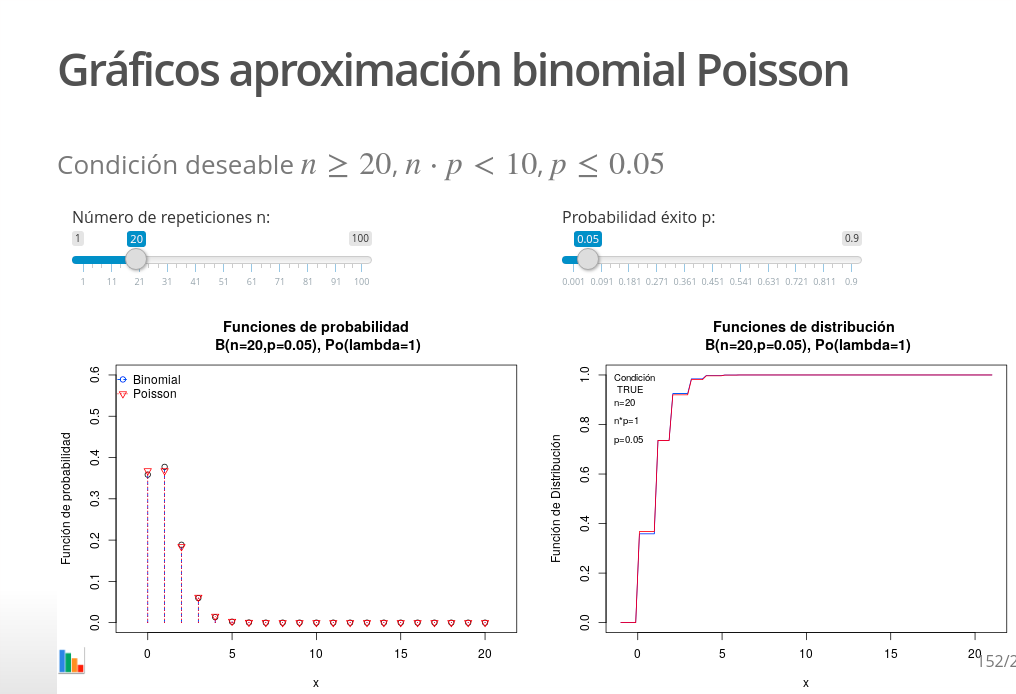
\includegraphics{Images/noshinyImages/interactiva_poisson1.png}}

\hypertarget{ejemplo-polambda}{%
\subsection{\texorpdfstring{Ejemplo \(Po(\lambda)\)}{Ejemplo Po(\textbackslash{}lambda)}}\label{ejemplo-polambda}}

\textbf{Ejemplo}: Trampa insectos.

La conocida \href{https://es.wikipedia.org/wiki/Insecticida_el\%C3\%A9ctrico}{lámpara antiinsectos o insecticida eléctrico} atrae a los insectos voladores con una luz ultravioleta y los mata por electrocución.

Consideremos la v.a. \(X\) que cuenta número de insectos caídos en la trampa en una hora. Supongamos que el número promedio de insectos que captura la trampa en una hora es \(E(X)=20\) y que podemos admitir que \(X\) sigue una ley de probabilidad \(Po(\lambda=20)\).

Nos piden

\begin{enumerate}
\def\labelenumi{\arabic{enumi}.}
\tightlist
\item
  Comentar de forma breve si se cumplen intuitivamente las condiciones para tener una distribución Poisson.
\item
  Escribir de forma explicita la función de probabilidad y de distribución de \(X\).
\item
  Calculad la probabilidad de que en una hora caigan en la trampa exactamente 21 insectos.
\item
  Calculad la probabilidad de que en una hora caigan en la trampa al menos 6 insectos.
\item
  ¿Cuál es el valor esperando, la varianza y la desviación típica de \(X\)?
\end{enumerate}

\hypertarget{ejemplo-polambda-1}{%
\subsection{\texorpdfstring{Ejemplo \(Po(\lambda)\)}{Ejemplo Po(\textbackslash{}lambda)}}\label{ejemplo-polambda-1}}

\textbf{Solución 1.} Comentar de forma breve si se cumplen intuitivamente las condiciones para tener una distribución Poisson.

\begin{enumerate}
\def\labelenumi{\arabic{enumi}.}
\tightlist
\item
  El número promedio de eventos en el intervalo \((0,1]\), una hora es
  \(\lambda=20>0\).
\item
  Es posible dividir el intervalo de tiempo de una hora en un
  gran número de subintervalos (denotemos por \(n\) al número de intervalos) de forma que:

  \begin{itemize}
  \tightlist
  \item
    La probabilidad de que se produzcan dos o más electrocuciones un subintervalo es despreciable. No es posible que dos mosquitos se electrocuten al mismo tiempo.
  \item
    El número de ocurrencias, electrocuciones de insectos, en un intervalo es independiente del número de electrocuciones en otro intervalo.
  \item
    La probabilidad de que un evento ocurra en un subintervalo es \(p_n\cdot n=\lambda\) o lo que es lo mismo \(p_n=\frac{\lambda}{n}\)· Podemos dividir los 20 insectos promedio entre los \(n\) intervalos (trozo de hora) de forma que \(p_n=\frac{\lambda}{n}\).
  \item
    Por ejemplo si \(n=60\) tenemos que \(p_n=\frac{20}{60}=\frac{1}{3}\). La probabilidad de que en un minuto la trampa chisporrotee es \(\frac{1}{3}\).
  \end{itemize}
\end{enumerate}

\hypertarget{ejemplo-polambda-2}{%
\subsection{\texorpdfstring{Ejemplo \(Po(\lambda)\)}{Ejemplo Po(\textbackslash{}lambda)}}\label{ejemplo-polambda-2}}

\textbf{Solución 2.} Escribid de forma explicita la función de probabilidad y de distribución de \(X\).

La distribución de probabilidad de un \(Po(\lambda)\) es

\[
P_X(x)=P(X=x)=\left\{\begin{array}{ll}  \frac{\lambda^x}{x!}e^{-\lambda} & \mbox{ si } x=0,1,\ldots\\ 0  & \mbox{ en otro caso.}\end{array}\right.
\]

Para un a \(Po(\lambda=20)\)

\[
P_X(x)=P(X=x)=\left\{\begin{array}{ll}\frac{20^x}{x!}e^{-20} & \mbox{ si } x=0,1,\ldots\\ 0  & \mbox{ en otro caso.}\end{array}\right.
\]

\hypertarget{ejemplo-polambda-3}{%
\subsection{\texorpdfstring{Ejemplo \(Po(\lambda)\)}{Ejemplo Po(\textbackslash{}lambda)}}\label{ejemplo-polambda-3}}

La función de distribución es

\[
F_X(x)=P(X\leq X)=
\left\{\begin{array}{ll} 
0 & \mbox{si } x<0\\
\displaystyle\sum_{i=0}^{k} P(X=i)=\sum_{i=0}^{k}\frac{\lambda^i}{i!}\cdot e^{-\lambda} & \mbox{si  }
\left\{\begin{array}{l}
k\leq x< k+1\\k=0,1,2,\ldots
\end{array}
\right.
\end{array}
\right.
\]

En nuestro caso
\[
F_X(x)=P(X\leq X)=
\left\{\begin{array}{ll} 
0 & \mbox{si } x<0\\
\displaystyle\sum_{i=0}^{k} P(X=i)=\sum_{i=0}^{k}\frac{20^i}{i!}\cdot e^{-20} & \mbox{si  }
\left\{\begin{array}{l}
k\leq x< k+1\\k=0,1,2,\ldots
\end{array}
\right.
\end{array}
\right.
\]

\hypertarget{ejemplo-polambda-4}{%
\subsection{\texorpdfstring{Ejemplo \(Po(\lambda)\)}{Ejemplo Po(\textbackslash{}lambda)}}\label{ejemplo-polambda-4}}

\textbf{Solución 3.} Calculad la probabilidad de que en una hora caigan en la trampa exactamente 21 insectos.

Nos piden

\[
P(X=21)=\frac{20^{21}}{21!}=0.0846051.
\]

Con R como calculadora y con la función de la distribución de R

\begin{Shaded}
\begin{Highlighting}[]
\DecValTok{20}\OperatorTok{^}\DecValTok{21}\OperatorTok{/}\KeywordTok{factorial}\NormalTok{(}\DecValTok{21}\NormalTok{)}\OperatorTok{*}\KeywordTok{exp}\NormalTok{(}\OperatorTok{-}\DecValTok{20}\NormalTok{)}
\end{Highlighting}
\end{Shaded}

\begin{verbatim}
## [1] 0.08460506
\end{verbatim}

\begin{Shaded}
\begin{Highlighting}[]
\KeywordTok{dpois}\NormalTok{(}\DecValTok{21}\NormalTok{,}\DataTypeTok{lambda =} \DecValTok{20}\NormalTok{)}
\end{Highlighting}
\end{Shaded}

\begin{verbatim}
## [1] 0.08460506
\end{verbatim}

\hypertarget{ejemplo-polambda-5}{%
\subsection{\texorpdfstring{Ejemplo \(Po(\lambda)\)}{Ejemplo Po(\textbackslash{}lambda)}}\label{ejemplo-polambda-5}}

\textbf{Solución 4.} Calculad la probabilidad de que en una hora caigan en la trampa al menos 6 insectos.

Nos piden
\[
\begin{eqnarray*}
 P(X\geq 6)&=&1- P(X<6)=1-P(X\leq 5)=1-F_X(5)=1-\displaystyle\sum_{x=0}^{5} \frac{20^{x}}{x!}\cdot e^{-20}\\
 &=&
 1-\left(\frac{20^{0}}{0!}\cdot e^{-20}+\frac{20^{1}}{1!}\cdot e^{-20}+\frac{20^{2}}{2!}\cdot e^{-20}+\frac{20^{3}}{3!}\cdot e^{-20}+\frac{20^{4}}{4!}\cdot e^{-20}+\frac{20^{5}}{5!}\cdot e^{-20}\right)\\
 &=&
 1-e^{-20}\cdot \left(1+20+\frac{400}{4}+\frac{8000}{6}+\frac{160000}{24}+\frac{3200000}{120}\right)\\
 &=&
 1-e^{-20} \cdot \left(\frac{1 \cdot 120+20\cdot 120+400\cdot 30+8000\cdot 20+160000\cdot 24+3200000\cdot 1}{120}\right)\\
 &=& 1-e^{-20}\cdot\left(\frac{4186520}{120}\right)=1-0.0066126.
\end{eqnarray*}
\]

\hypertarget{ejemplo-polambda-6}{%
\subsection{\texorpdfstring{Ejemplo \(Po(\lambda)\)}{Ejemplo Po(\textbackslash{}lambda)}}\label{ejemplo-polambda-6}}

\textbf{Solución 5.} ¿Cuál es el valor esperado, la varianza y la desviación típica de \(X\)?

El valor esperado del número de insectos caídos en la trampa en una hora es

\[E(X)=\lambda=20\]

Su varianza es
\[Var(X)=\lambda=20\]

y su desviación típica vale
\[\sqrt{Var(X)}=+\sqrt{\lambda}=+\sqrt{20}.\]

\hypertarget{cuxe1lculos-con-r-4}{%
\subsection{Cálculos con R}\label{cuxe1lculos-con-r-4}}

Sea \(X\) un una v.a. \(Po(\lambda=3)\). Entonces \(P_X(0)=P(X=0), P_X(1)=P(X=1)\):

\begin{Shaded}
\begin{Highlighting}[]
\KeywordTok{dpois}\NormalTok{(}\DecValTok{0}\NormalTok{,}\DataTypeTok{lambda =} \DecValTok{3}\NormalTok{)}
\end{Highlighting}
\end{Shaded}

\begin{verbatim}
## [1] 0.04978707
\end{verbatim}

\begin{Shaded}
\begin{Highlighting}[]
\KeywordTok{dpois}\NormalTok{(}\DecValTok{1}\NormalTok{,}\DataTypeTok{lambda =} \DecValTok{3}\NormalTok{)}
\end{Highlighting}
\end{Shaded}

\begin{verbatim}
## [1] 0.1493612
\end{verbatim}

\hypertarget{cuxe1lculos-con-r-5}{%
\subsection{Cálculos con R}\label{cuxe1lculos-con-r-5}}

\(F_X(0)=P(X\leq 0), F_X(1)=P(X\leq 1)\):

\begin{Shaded}
\begin{Highlighting}[]
\KeywordTok{ppois}\NormalTok{(}\DecValTok{0}\NormalTok{,}\DataTypeTok{lambda =} \DecValTok{3}\NormalTok{)}
\end{Highlighting}
\end{Shaded}

\begin{verbatim}
## [1] 0.04978707
\end{verbatim}

\begin{Shaded}
\begin{Highlighting}[]
\KeywordTok{ppois}\NormalTok{(}\DecValTok{1}\NormalTok{,}\DataTypeTok{lambda =} \DecValTok{3}\NormalTok{)}
\end{Highlighting}
\end{Shaded}

\begin{verbatim}
## [1] 0.1991483
\end{verbatim}

\begin{Shaded}
\begin{Highlighting}[]
\KeywordTok{dpois}\NormalTok{(}\DecValTok{0}\NormalTok{,}\DataTypeTok{lambda =} \DecValTok{3}\NormalTok{)}\OperatorTok{+}\KeywordTok{dpois}\NormalTok{(}\DecValTok{1}\NormalTok{,}\DataTypeTok{lambda =} \DecValTok{3}\NormalTok{) }\CommentTok{### es igual a ppois(1,lambda=3)}
\end{Highlighting}
\end{Shaded}

\begin{verbatim}
## [1] 0.1991483
\end{verbatim}

\hypertarget{cuxe1lculos-con-r-6}{%
\subsection{Cálculos con R}\label{cuxe1lculos-con-r-6}}

Por ejemplo podemos comprobar que \(F_X(10)=\sum_{x=0}^{10} P_X(x)\)

\begin{Shaded}
\begin{Highlighting}[]
\KeywordTok{dpois}\NormalTok{(}\DecValTok{0}\OperatorTok{:}\DecValTok{10}\NormalTok{,}\DecValTok{3}\NormalTok{)}
\end{Highlighting}
\end{Shaded}

\begin{verbatim}
##  [1] 0.0497870684 0.1493612051 0.2240418077 0.2240418077 0.1680313557
##  [6] 0.1008188134 0.0504094067 0.0216040315 0.0081015118 0.0027005039
## [11] 0.0008101512
\end{verbatim}

\begin{Shaded}
\begin{Highlighting}[]
\KeywordTok{sum}\NormalTok{(}\KeywordTok{dpois}\NormalTok{(}\DecValTok{0}\OperatorTok{:}\DecValTok{10}\NormalTok{,}\DecValTok{3}\NormalTok{))}
\end{Highlighting}
\end{Shaded}

\begin{verbatim}
## [1] 0.9997077
\end{verbatim}

\begin{Shaded}
\begin{Highlighting}[]
\KeywordTok{ppois}\NormalTok{(}\DecValTok{10}\NormalTok{,}\DecValTok{3}\NormalTok{)}
\end{Highlighting}
\end{Shaded}

\begin{verbatim}
## [1] 0.9997077
\end{verbatim}

\hypertarget{cuxe1lculos-distribuciuxf3n-poisson-con-r}{%
\subsection{Cálculos distribución Poisson con R}\label{cuxe1lculos-distribuciuxf3n-poisson-con-r}}

Y también generar secuencias de observaciones aleatorias de una población \(Po(3)\)

\begin{Shaded}
\begin{Highlighting}[]
\KeywordTok{rpois}\NormalTok{(}\DataTypeTok{n=}\DecValTok{100}\NormalTok{,}\DataTypeTok{lambda =} \DecValTok{3}\NormalTok{)}
\end{Highlighting}
\end{Shaded}

\begin{verbatim}
##   [1] 2 5 3 3 2 2 5 2 4 4 2 3 2 2 2 2 2 3 3 5 3 3 2 4 2 3 2 1 1 3 4 6 2 5 3 4 1
##  [38] 1 6 3 4 1 4 3 4 3 0 2 1 4 3 0 2 4 2 3 5 2 1 3 3 4 2 5 0 3 1 1 4 6 4 5 0 4
##  [75] 0 3 3 3 4 1 2 6 2 2 2 2 1 2 5 2 5 3 7 3 5 2 3 2 1 3
\end{verbatim}

\hypertarget{cuxe1lculos-con-r-7}{%
\subsection{Cálculos con R}\label{cuxe1lculos-con-r-7}}

En el ejercicio de la trampa para insectos teníamos que \(X\) es una \(Po(20)\). Responded con R a la preguntas 3 y 4 de este ejercicio

\textbf{Pregunta 3.} Calculad la probabilidad de que en una hora caigan en la trampa exactamente 21 insectos.

La respuesta a la pregunta 3 es calcular \(P(X=21)\)

\begin{Shaded}
\begin{Highlighting}[]
\KeywordTok{dpois}\NormalTok{(}\DecValTok{21}\NormalTok{,}\DataTypeTok{lambda=}\DecValTok{20}\NormalTok{)}\CommentTok{## P(X=21)}
\end{Highlighting}
\end{Shaded}

\begin{verbatim}
## [1] 0.08460506
\end{verbatim}

\hypertarget{cuxe1lculos-con-r-8}{%
\subsection{Cálculos con R}\label{cuxe1lculos-con-r-8}}

\textbf{Pregunta 4.} Calculad la probabilidad de que en una hora caigan en la trampa al menos 6 insectos.

La pregunta 4 nos pide calcular \(P(X\geq 6)=1-P(X<6)=1-P(X\leq 5)\)

\begin{Shaded}
\begin{Highlighting}[]
\KeywordTok{ppois}\NormalTok{(}\DecValTok{5}\NormalTok{,}\DataTypeTok{lambda=}\DecValTok{20}\NormalTok{)}
\end{Highlighting}
\end{Shaded}

\begin{verbatim}
## [1] 7.190884e-05
\end{verbatim}

\begin{Shaded}
\begin{Highlighting}[]
\DecValTok{1}\OperatorTok{-}\KeywordTok{ppois}\NormalTok{(}\DecValTok{5}\NormalTok{,}\DataTypeTok{lambda=}\DecValTok{20}\NormalTok{) }\CommentTok{## es 1-P(X<=5)=P(X>=6)}
\end{Highlighting}
\end{Shaded}

\begin{verbatim}
## [1] 0.9999281
\end{verbatim}

\begin{Shaded}
\begin{Highlighting}[]
\KeywordTok{ppois}\NormalTok{(}\DecValTok{5}\NormalTok{,}\DataTypeTok{lambda=}\DecValTok{20}\NormalTok{,}\DataTypeTok{lower.tail =}\OtherTok{FALSE}\NormalTok{ ) }\CommentTok{## acumula hacia arriba P(X>5)=P(X>=6)=P(X=6)+P(X=7)+...}
\end{Highlighting}
\end{Shaded}

\begin{verbatim}
## [1] 0.9999281
\end{verbatim}

\hypertarget{gruxe1ficos-de-la-distribuciuxf3n-poisson-con-r}{%
\subsection{Gráficos de la distribución Poisson con R}\label{gruxe1ficos-de-la-distribuciuxf3n-poisson-con-r}}

\begin{Shaded}
\begin{Highlighting}[]
\NormalTok{lambda=}\DecValTok{20}
\KeywordTok{par}\NormalTok{(}\DataTypeTok{mfrow=}\KeywordTok{c}\NormalTok{(}\DecValTok{1}\NormalTok{,}\DecValTok{2}\NormalTok{))}
\NormalTok{n=}\KeywordTok{qpois}\NormalTok{(}\FloatTok{0.99}\NormalTok{,}\DataTypeTok{lambda=}\NormalTok{lambda)}
\NormalTok{aux=}\KeywordTok{rep}\NormalTok{(}\DecValTok{0}\NormalTok{,(n}\OperatorTok{+}\DecValTok{1}\NormalTok{)}\OperatorTok{*}\DecValTok{2}\NormalTok{)}
\NormalTok{aux[}\KeywordTok{seq}\NormalTok{(}\DecValTok{2}\NormalTok{,(n}\OperatorTok{+}\DecValTok{1}\NormalTok{)}\OperatorTok{*}\DecValTok{2}\NormalTok{,}\DecValTok{2}\NormalTok{)]=}\KeywordTok{dpois}\NormalTok{(}\KeywordTok{c}\NormalTok{(}\DecValTok{0}\OperatorTok{:}\NormalTok{n),}\DataTypeTok{lambda=}\NormalTok{lambda)}
\NormalTok{ymax=}\KeywordTok{max}\NormalTok{(}\KeywordTok{ppois}\NormalTok{(}\DecValTok{0}\OperatorTok{:}\NormalTok{n,}\DataTypeTok{lambda=}\NormalTok{lambda))}
\KeywordTok{plot}\NormalTok{(}\DataTypeTok{x=}\KeywordTok{c}\NormalTok{(}\DecValTok{0}\OperatorTok{:}\NormalTok{n),}\DataTypeTok{y=}\KeywordTok{dpois}\NormalTok{(}\KeywordTok{c}\NormalTok{(}\DecValTok{0}\OperatorTok{:}\NormalTok{n),}\DataTypeTok{lambda=}\NormalTok{lambda),}
     \DataTypeTok{ylim=}\KeywordTok{c}\NormalTok{(}\DecValTok{0}\NormalTok{,ymax),}\DataTypeTok{xlim=}\KeywordTok{c}\NormalTok{(}\OperatorTok{-}\DecValTok{1}\NormalTok{,n}\OperatorTok{+}\DecValTok{1}\NormalTok{),}\DataTypeTok{xlab=}\StringTok{"x"}\NormalTok{,}\DataTypeTok{ylab=}\StringTok{"Función de probabilidad"}\NormalTok{,}
     \DataTypeTok{main=}\KeywordTok{paste0}\NormalTok{(}\KeywordTok{c}\NormalTok{(}\StringTok{"Función de probabilidad}\CharTok{\textbackslash{}n}\StringTok{  Po(lambda="}\NormalTok{,lambda,}\StringTok{")"}\NormalTok{),}\DataTypeTok{collapse =} \StringTok{""}\NormalTok{))}
\KeywordTok{lines}\NormalTok{(}\DataTypeTok{x=}\KeywordTok{rep}\NormalTok{(}\DecValTok{0}\OperatorTok{:}\NormalTok{n,}\DataTypeTok{each=}\DecValTok{2}\NormalTok{),}\DataTypeTok{y=}\NormalTok{aux,}\DataTypeTok{pch=}\DecValTok{21}\NormalTok{, }\DataTypeTok{type =} \StringTok{"h"}\NormalTok{, }\DataTypeTok{lty =} \DecValTok{2}\NormalTok{,}\DataTypeTok{col=}\StringTok{"blue"}\NormalTok{)}
\KeywordTok{curve}\NormalTok{(}\KeywordTok{ppois}\NormalTok{(x,}\DataTypeTok{lambda=}\NormalTok{lambda),}
      \DataTypeTok{xlim=}\KeywordTok{c}\NormalTok{(}\OperatorTok{-}\DecValTok{1}\NormalTok{,n}\OperatorTok{+}\DecValTok{1}\NormalTok{),}\DataTypeTok{col=}\StringTok{"blue"}\NormalTok{,}\DataTypeTok{ylab=}\StringTok{"Función de Distribución",}
\StringTok{      main=paste0(c("}\NormalTok{Función de distribución \textbackslash{}n }\KeywordTok{Po}\NormalTok{(}\DataTypeTok{lambda=}\StringTok{",lambda,"}\NormalTok{)}\StringTok{"),collapse = ""))}
\StringTok{par(mfrow=c(1,1))}
\end{Highlighting}
\end{Shaded}

\hypertarget{gruxe1ficos-de-la-distribuciuxf3n-poisson-con-r-1}{%
\subsection{Gráficos de la distribución Poisson con R}\label{gruxe1ficos-de-la-distribuciuxf3n-poisson-con-r-1}}

\begin{center}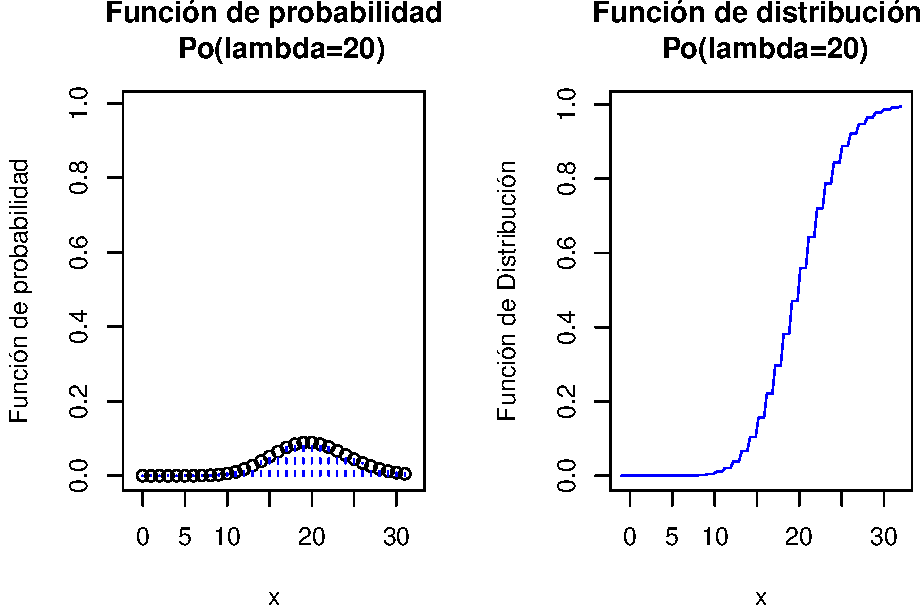
\includegraphics{curso-probabilidad-udemy_files/figure-latex/graficosPOISON-1} \end{center}

\hypertarget{gruxe1ficos-interactivos-con-r}{%
\subsection{Gráficos interactivos con R}\label{gruxe1ficos-interactivos-con-r}}

Para ejecutar el siguiente gráfico interactivo, solamente tienes que cargar el paquete \texttt{shiny} en tu ordenador y luego copiar/pegar las siguientes instrucciones. De este modo podrás observar los cambios en las distribuciones variando los parámetros.

\begin{Shaded}
\begin{Highlighting}[]
\KeywordTok{sliderInput}\NormalTok{(}\StringTok{"lambda"}\NormalTok{, }\DataTypeTok{label =} \StringTok{"Promedio de eventos lambda"}\NormalTok{,}
              \DataTypeTok{min =} \DecValTok{1}\NormalTok{, }\DataTypeTok{max =} \DecValTok{100}\NormalTok{, }\DataTypeTok{value =}\DecValTok{20}\NormalTok{ , }\DataTypeTok{step =} \DecValTok{1}\NormalTok{)}
\KeywordTok{renderPlot}\NormalTok{(\{}
\NormalTok{  lambda=input}\OperatorTok{$}\NormalTok{lambda}
  \KeywordTok{par}\NormalTok{(}\DataTypeTok{mfrow=}\KeywordTok{c}\NormalTok{(}\DecValTok{1}\NormalTok{,}\DecValTok{2}\NormalTok{))}
\NormalTok{  n=}\KeywordTok{qpois}\NormalTok{(}\FloatTok{0.99}\NormalTok{,}\DataTypeTok{lambda=}\NormalTok{lambda)}
  \CommentTok{#n}
\NormalTok{  aux=}\KeywordTok{rep}\NormalTok{(}\DecValTok{0}\NormalTok{,(n}\OperatorTok{+}\DecValTok{1}\NormalTok{)}\OperatorTok{*}\DecValTok{2}\NormalTok{)}
\NormalTok{  aux[}\KeywordTok{seq}\NormalTok{(}\DecValTok{2}\NormalTok{,(n}\OperatorTok{+}\DecValTok{1}\NormalTok{)}\OperatorTok{*}\DecValTok{2}\NormalTok{,}\DecValTok{2}\NormalTok{)]=}\KeywordTok{dpois}\NormalTok{(}\KeywordTok{c}\NormalTok{(}\DecValTok{0}\OperatorTok{:}\NormalTok{n),}\DataTypeTok{lambda=}\NormalTok{lambda)}
\NormalTok{  ymax=}\FloatTok{0.45}
  \KeywordTok{plot}\NormalTok{(}\DataTypeTok{x=}\KeywordTok{c}\NormalTok{(}\DecValTok{0}\OperatorTok{:}\NormalTok{n),}\DataTypeTok{y=}\KeywordTok{dpois}\NormalTok{(}\KeywordTok{c}\NormalTok{(}\DecValTok{0}\OperatorTok{:}\NormalTok{n),}\DataTypeTok{lambda=}\NormalTok{lambda),}
       \DataTypeTok{ylim=}\KeywordTok{c}\NormalTok{(}\DecValTok{0}\NormalTok{,ymax),}\DataTypeTok{xlim=}\KeywordTok{c}\NormalTok{(}\OperatorTok{-}\DecValTok{1}\NormalTok{,n}\OperatorTok{+}\DecValTok{1}\NormalTok{),}\DataTypeTok{xlab=}\StringTok{"x"}\NormalTok{,}\DataTypeTok{ylab=}\StringTok{"Función de probabilidad"}\NormalTok{,}
       \DataTypeTok{main=}\KeywordTok{paste0}\NormalTok{(}\KeywordTok{c}\NormalTok{(}\StringTok{"Función de probabilidad}\CharTok{\textbackslash{}n}\StringTok{  Po(lambda="}\NormalTok{,lambda,}\StringTok{")"}\NormalTok{),}\DataTypeTok{collapse =} \StringTok{""}\NormalTok{))}
  \KeywordTok{lines}\NormalTok{(}\DataTypeTok{x=}\KeywordTok{rep}\NormalTok{(}\DecValTok{0}\OperatorTok{:}\NormalTok{n,}\DataTypeTok{each=}\DecValTok{2}\NormalTok{),}\DataTypeTok{y=}\NormalTok{aux,}\DataTypeTok{pch=}\DecValTok{21}\NormalTok{, }\DataTypeTok{type =} \StringTok{"h"}\NormalTok{, }\DataTypeTok{lty =} \DecValTok{2}\NormalTok{,}\DataTypeTok{col=}\StringTok{"blue"}\NormalTok{)}
  \KeywordTok{curve}\NormalTok{(}\KeywordTok{ppois}\NormalTok{(x,}\DataTypeTok{lambda=}\NormalTok{lambda),}
        \DataTypeTok{xlim=}\KeywordTok{c}\NormalTok{(}\OperatorTok{-}\DecValTok{1}\NormalTok{,n}\OperatorTok{+}\DecValTok{1}\NormalTok{),}\DataTypeTok{col=}\StringTok{"blue"}\NormalTok{,}\DataTypeTok{ylab=}\StringTok{"Función de Distribución",}
\StringTok{         main=paste0(c("}\NormalTok{Función de distribución \textbackslash{}n }\KeywordTok{Po}\NormalTok{(}\DataTypeTok{lambda=}\StringTok{",lambda,"}\NormalTok{)}\StringTok{"),collapse = ""))}
\StringTok{  par(mfrow=c(1,1))}
\StringTok{\})}
\end{Highlighting}
\end{Shaded}

\href{https://joanby.shinyapps.io/DistribucionesNotables/}{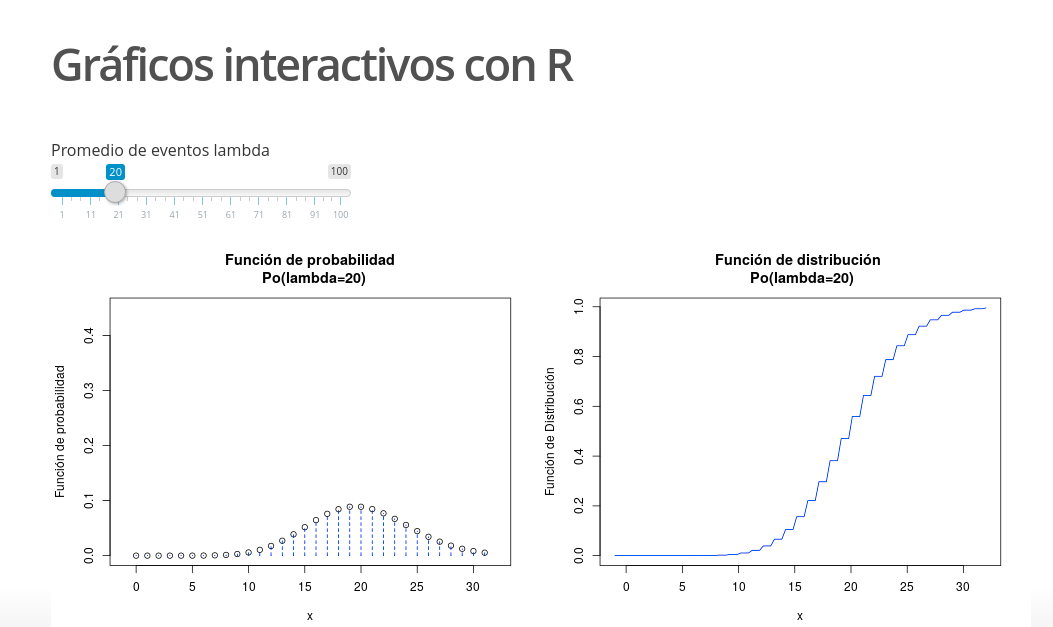
\includegraphics{Images/noshinyImages/interactiva_poisson2.png}}

\hypertarget{cuxe1lculos-con-python-6}{%
\subsection{Cálculos con python}\label{cuxe1lculos-con-python-6}}

Sea \(X\) un una v.a. \(Po(\lambda=3)\). Entonces

\(P_X(0)=P(X=0), P_X(1)=P(X=1)\) en este orden son

\begin{Shaded}
\begin{Highlighting}[]
\ImportTok{from}\NormalTok{ scipy.stats }\ImportTok{import}\NormalTok{ poisson}
\NormalTok{poisson.pmf(}\DecValTok{0}\NormalTok{,mu }\OperatorTok{=} \DecValTok{3}\NormalTok{)}
\end{Highlighting}
\end{Shaded}

\begin{verbatim}
## 0.049787068367863944
\end{verbatim}

\begin{Shaded}
\begin{Highlighting}[]
\NormalTok{poisson.pmf(}\DecValTok{1}\NormalTok{,mu }\OperatorTok{=} \DecValTok{3}\NormalTok{)}
\end{Highlighting}
\end{Shaded}

\begin{verbatim}
## 0.14936120510359185
\end{verbatim}

\hypertarget{cuxe1lculos-con-python-7}{%
\subsection{Cálculos con python}\label{cuxe1lculos-con-python-7}}

Sea \(X\) un una v.a. \(Po(\lambda=3)\). Entonces

\(F_X(0)=P(X\leq 0), F_X(1)=P(X\leq 1)\) en este orden son

\begin{Shaded}
\begin{Highlighting}[]
\NormalTok{poisson.cdf(}\DecValTok{0}\NormalTok{,mu }\OperatorTok{=} \DecValTok{3}\NormalTok{)}
\end{Highlighting}
\end{Shaded}

\begin{verbatim}
## 0.049787068367863951
\end{verbatim}

\begin{Shaded}
\begin{Highlighting}[]
\NormalTok{poisson.cdf(}\DecValTok{1}\NormalTok{,mu }\OperatorTok{=} \DecValTok{3}\NormalTok{)}
\end{Highlighting}
\end{Shaded}

\begin{verbatim}
## 0.19914827347145581
\end{verbatim}

\begin{Shaded}
\begin{Highlighting}[]
\NormalTok{poisson.pmf(}\DecValTok{0}\NormalTok{,mu }\OperatorTok{=} \DecValTok{3}\NormalTok{)}\OperatorTok{+}\NormalTok{poisson.pmf(}\DecValTok{1}\NormalTok{,mu}\OperatorTok{=} \DecValTok{3}\NormalTok{) }\CommentTok{### es igual a poisson.cdf(1,lambda=3)}
\end{Highlighting}
\end{Shaded}

\begin{verbatim}
## 0.19914827347145581
\end{verbatim}

\hypertarget{cuxe1lculos-con-python-8}{%
\subsection{Cálculos con python}\label{cuxe1lculos-con-python-8}}

Por ejemplo podemos comprobar que \(F_X(10)=\displaystyle\sum_{0}^{10} P_X(x)\)

\begin{Shaded}
\begin{Highlighting}[]
\BuiltInTok{range}\NormalTok{(}\DecValTok{0}\NormalTok{,}\DecValTok{10}\NormalTok{)}
\end{Highlighting}
\end{Shaded}

\begin{verbatim}
## [0, 1, 2, 3, 4, 5, 6, 7, 8, 9]
\end{verbatim}

\begin{Shaded}
\begin{Highlighting}[]
\NormalTok{poisson.pmf(}\BuiltInTok{range}\NormalTok{(}\DecValTok{0}\NormalTok{,}\DecValTok{10}\NormalTok{),mu}\OperatorTok{=}\DecValTok{3}\NormalTok{)}
\end{Highlighting}
\end{Shaded}

\begin{verbatim}
## array([ 0.04978707,  0.14936121,  0.22404181,  0.22404181,  0.16803136,
##         0.10081881,  0.05040941,  0.02160403,  0.00810151,  0.0027005 ])
\end{verbatim}

\begin{Shaded}
\begin{Highlighting}[]
\BuiltInTok{sum}\NormalTok{(poisson.pmf(}\BuiltInTok{range}\NormalTok{(}\DecValTok{0}\NormalTok{,}\DecValTok{10}\NormalTok{),mu}\OperatorTok{=}\DecValTok{3}\NormalTok{))}
\end{Highlighting}
\end{Shaded}

\begin{verbatim}
## 0.99889751186988462
\end{verbatim}

\begin{Shaded}
\begin{Highlighting}[]
\NormalTok{poisson.cdf(}\DecValTok{10}\NormalTok{,mu}\OperatorTok{=}\DecValTok{3}\NormalTok{)}
\end{Highlighting}
\end{Shaded}

\begin{verbatim}
## 0.99970766304935266
\end{verbatim}

\hypertarget{cuxe1lculos-con-python-9}{%
\subsection{Cálculos con python}\label{cuxe1lculos-con-python-9}}

En el ejercicio de la trampa para insectos teníamos que \(X\) es una \(Po(20)\). Responded con python a la preguntas 3 y 4 de este ejercicio

\textbf{Pregunta 3.} Calculad la probabilidad de que en una hora caigan en la trampa exactamente 21 insectos.

La respuesta a la pregunta 3 es calcular \(P(X=21)\)

\begin{Shaded}
\begin{Highlighting}[]
\NormalTok{poisson.pmf(}\DecValTok{21}\NormalTok{,mu}\OperatorTok{=}\DecValTok{20}\NormalTok{)}
\CommentTok{## P(X=21)}
\end{Highlighting}
\end{Shaded}

\begin{verbatim}
## 0.084605064182937909
\end{verbatim}

\hypertarget{cuxe1lculos-con-r-9}{%
\subsection{Cálculos con R}\label{cuxe1lculos-con-r-9}}

\textbf{Pregunta 4.} Calculad la probabilidad de que en una hora caigan en la trampa al menos 6 insectos.

La pregunta 4 nos pide calcular \(P(X\geq 6)=1-P(X\leq 5)\)

\begin{Shaded}
\begin{Highlighting}[]
\DecValTok{1}\OperatorTok{-}\NormalTok{poisson.cdf(}\DecValTok{5}\NormalTok{,mu}\OperatorTok{=}\DecValTok{20}\NormalTok{) }
\CommentTok{## es 1-P(X<=5)=P(X>=6)}
\end{Highlighting}
\end{Shaded}

\begin{verbatim}
## 0.99992809115947157
\end{verbatim}

\hypertarget{cuxe1lculos-con-python-10}{%
\subsection{Cálculos con python}\label{cuxe1lculos-con-python-10}}

Como ya hemos visto con \texttt{scipy.stats} podemos pedir los momentos de una variable aleatoria
\(Po(3)\)

\begin{Shaded}
\begin{Highlighting}[]
\NormalTok{poisson.stats(mu}\OperatorTok{=}\DecValTok{3}\NormalTok{, moments}\OperatorTok{=}\StringTok{'mv'}\NormalTok{)}
\end{Highlighting}
\end{Shaded}

\begin{verbatim}
## (array(3.0), array(3.0))
\end{verbatim}

Y también generar secuencias de observaciones aleatorias de una población \(Po(3)\)

\begin{Shaded}
\begin{Highlighting}[]
\NormalTok{poisson.rvs(mu}\OperatorTok{=}\DecValTok{3}\NormalTok{,size}\OperatorTok{=}\DecValTok{40}\NormalTok{)}
\end{Highlighting}
\end{Shaded}

\begin{verbatim}
## array([3, 1, 4, 5, 3, 0, 4, 3, 1, 1, 7, 2, 2, 3, 2, 4, 6, 3, 1, 3, 4, 1, 1,
##        1, 2, 4, 2, 2, 3, 3, 4, 3, 7, 3, 2, 4, 4, 2, 1, 1])
\end{verbatim}

\hypertarget{gruxe1ficos-con-python-2}{%
\subsection{Gráficos con python}\label{gruxe1ficos-con-python-2}}

\begin{Shaded}
\begin{Highlighting}[]
\ImportTok{from}\NormalTok{ scipy.stats }\ImportTok{import}\NormalTok{ poisson}
\NormalTok{mu }\OperatorTok{=} \DecValTok{10} \CommentTok{## mu = lambda}
\NormalTok{x }\OperatorTok{=}\NormalTok{ np.arange(poisson.ppf(}\FloatTok{0.01}\NormalTok{, mu),poisson.ppf(}\FloatTok{0.99}\NormalTok{, mu))}
\NormalTok{fig }\OperatorTok{=}\NormalTok{plt.figure(figsize}\OperatorTok{=}\NormalTok{(}\DecValTok{5}\NormalTok{, }\FloatTok{2.7}\NormalTok{))}
\NormalTok{ax }\OperatorTok{=}\NormalTok{ fig.add_subplot(}\DecValTok{1}\NormalTok{,}\DecValTok{2}\NormalTok{,}\DecValTok{1}\NormalTok{)}
\NormalTok{ax.plot(x, poisson.pmf(x, mu), }\StringTok{'bo'}\NormalTok{, ms}\OperatorTok{=}\DecValTok{5}\NormalTok{, label}\OperatorTok{=}\StringTok{'poisson pmf'}\NormalTok{)}
\NormalTok{ax.vlines(x, }\DecValTok{0}\NormalTok{, poisson.pmf(x, mu), colors}\OperatorTok{=}\StringTok{'b'}\NormalTok{, lw}\OperatorTok{=}\DecValTok{2}\NormalTok{, alpha}\OperatorTok{=}\FloatTok{0.5}\NormalTok{)}
\ControlFlowTok{for}\NormalTok{ tick }\KeywordTok{in}\NormalTok{ ax.xaxis.get_major_ticks():}
\NormalTok{  tick.label.set_fontsize(}\DecValTok{5}\NormalTok{)}
\ControlFlowTok{for}\NormalTok{ tick }\KeywordTok{in}\NormalTok{ ax.yaxis.get_major_ticks():}
\NormalTok{  tick.label.set_fontsize(}\DecValTok{5}\NormalTok{) }
\NormalTok{ax }\OperatorTok{=}\NormalTok{ fig.add_subplot(}\DecValTok{1}\NormalTok{,}\DecValTok{2}\NormalTok{,}\DecValTok{2}\NormalTok{)}
\NormalTok{ax.plot(x, poisson.cdf(x, mu), }\StringTok{'bo'}\NormalTok{, ms}\OperatorTok{=}\DecValTok{5}\NormalTok{, label}\OperatorTok{=}\StringTok{'poisson cdf'}\NormalTok{)}
\NormalTok{ax.vlines(x, }\DecValTok{0}\NormalTok{, poisson.cdf(x, mu), colors}\OperatorTok{=}\StringTok{'b'}\NormalTok{, lw}\OperatorTok{=}\DecValTok{2}\NormalTok{, alpha}\OperatorTok{=}\FloatTok{0.5}\NormalTok{)}
\ControlFlowTok{for}\NormalTok{ tick }\KeywordTok{in}\NormalTok{ ax.xaxis.get_major_ticks():}
\NormalTok{  tick.label.set_fontsize(}\DecValTok{5}\NormalTok{)}
\ControlFlowTok{for}\NormalTok{ tick }\KeywordTok{in}\NormalTok{ ax.yaxis.get_major_ticks():}
\NormalTok{  tick.label.set_fontsize(}\DecValTok{5}\NormalTok{)}
\NormalTok{fig.suptitle(}\StringTok{'Distribucion de Poisson'}\NormalTok{)}
\NormalTok{plt.show()}
\end{Highlighting}
\end{Shaded}

\hypertarget{gruxe1ficos-con-python-3}{%
\subsection{Gráficos con python}\label{gruxe1ficos-con-python-3}}

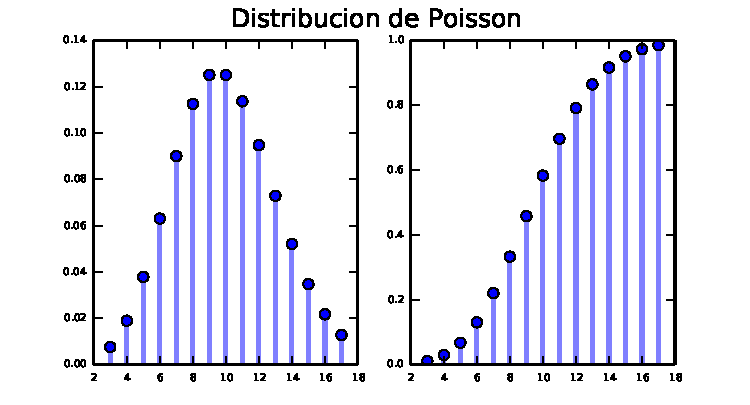
\includegraphics{curso-probabilidad-udemy_files/figure-latex/py_poiss2-1.pdf}

\hypertarget{gruxe1ficos-interactivos-proceso-polambdacdot-t}{%
\subsection{\texorpdfstring{Gráficos interactivos proceso \(Po(\lambda\cdot t\))}{Gráficos interactivos proceso Po(\textbackslash{}lambda\textbackslash{}cdot t)}}\label{gruxe1ficos-interactivos-proceso-polambdacdot-t}}

Para ejecutar el siguiente gráfico interactivo, solamente tienes que cargar el paquete \texttt{shiny} en tu ordenador y luego copiar/pegar las siguientes instrucciones. De este modo podrás observar los cambios en las distribuciones variando los parámetros.

\begin{Shaded}
\begin{Highlighting}[]
\KeywordTok{fluidPage}\NormalTok{(}
  \KeywordTok{fluidRow}\NormalTok{(}
      \KeywordTok{column}\NormalTok{(}\DecValTok{6}\NormalTok{,}
           \KeywordTok{sliderInput}\NormalTok{(}\StringTok{"lambdapp"}\NormalTok{, }\DataTypeTok{label=}\StringTok{"Promedio eventos por unidad de tiempo"}\NormalTok{, }\DataTypeTok{min =} \FloatTok{0.1}\NormalTok{, }\DataTypeTok{max =} \DecValTok{50}\NormalTok{, }\DataTypeTok{value =}\DecValTok{10}\NormalTok{ , }\DataTypeTok{step =} \FloatTok{0.01}\NormalTok{)),}
    \KeywordTok{column}\NormalTok{(}\DecValTok{6}\NormalTok{,}\KeywordTok{sliderInput}\NormalTok{(}\StringTok{"t"}\NormalTok{, }\DataTypeTok{label =} \StringTok{"Intervalo de tiempo (0,t]"}\NormalTok{, }\DataTypeTok{min =} \DecValTok{1}\NormalTok{, }\DataTypeTok{max =} \DecValTok{120}\NormalTok{, }\DataTypeTok{value =}\DecValTok{1}\NormalTok{ , }\DataTypeTok{step =} \FloatTok{0.5}\NormalTok{))}
\NormalTok{   )}
\NormalTok{)}


\KeywordTok{renderPlot}\NormalTok{(\{}
\NormalTok{  lambda1=input}\OperatorTok{$}\NormalTok{lambdapp}
\NormalTok{  t=input}\OperatorTok{$}\NormalTok{t}
\NormalTok{  lambda=lambda1}\OperatorTok{*}\NormalTok{t }\CommentTok{## es lambda* t}
  \KeywordTok{par}\NormalTok{(}\DataTypeTok{mfrow=}\KeywordTok{c}\NormalTok{(}\DecValTok{1}\NormalTok{,}\DecValTok{2}\NormalTok{))}
\NormalTok{  n=}\KeywordTok{qpois}\NormalTok{(}\FloatTok{0.99}\NormalTok{,}\DataTypeTok{lambda=}\NormalTok{lambda)}
  \CommentTok{#n}
\NormalTok{  aux=}\KeywordTok{rep}\NormalTok{(}\DecValTok{0}\NormalTok{,(n}\OperatorTok{+}\DecValTok{1}\NormalTok{)}\OperatorTok{*}\DecValTok{2}\NormalTok{)}
\NormalTok{  aux[}\KeywordTok{seq}\NormalTok{(}\DecValTok{2}\NormalTok{,(n}\OperatorTok{+}\DecValTok{1}\NormalTok{)}\OperatorTok{*}\DecValTok{2}\NormalTok{,}\DecValTok{2}\NormalTok{)]=}\KeywordTok{dpois}\NormalTok{(}\KeywordTok{c}\NormalTok{(}\DecValTok{0}\OperatorTok{:}\NormalTok{n),}\DataTypeTok{lambda=}\NormalTok{lambda)}
\NormalTok{  ymax=}\KeywordTok{ppois}\NormalTok{(}\KeywordTok{which.max}\NormalTok{(}\KeywordTok{ppois}\NormalTok{(}\DecValTok{0}\OperatorTok{:}\NormalTok{n,lambda))}\OperatorTok{-}\DecValTok{1}\NormalTok{,lambda)}\OperatorTok{*}\FloatTok{0.7}
  \KeywordTok{plot}\NormalTok{(}\DataTypeTok{x=}\KeywordTok{c}\NormalTok{(}\DecValTok{0}\OperatorTok{:}\NormalTok{n),}\DataTypeTok{y=}\KeywordTok{dpois}\NormalTok{(}\KeywordTok{c}\NormalTok{(}\DecValTok{0}\OperatorTok{:}\NormalTok{n),}\DataTypeTok{lambda=}\NormalTok{lambda),}
       \DataTypeTok{ylim=}\KeywordTok{c}\NormalTok{(}\DecValTok{0}\NormalTok{,ymax),}\DataTypeTok{xlim=}\KeywordTok{c}\NormalTok{(}\OperatorTok{-}\DecValTok{1}\NormalTok{,n}\OperatorTok{+}\DecValTok{1}\NormalTok{),}\DataTypeTok{xlab=}\StringTok{"x"}\NormalTok{,}\DataTypeTok{ylab=}\StringTok{"Función de probabilidad"}\NormalTok{,}
       \DataTypeTok{main=}\KeywordTok{paste0}\NormalTok{(}\KeywordTok{c}\NormalTok{(}\StringTok{"Función de probabilidad}\CharTok{\textbackslash{}n}\StringTok{  Po(lambda="}\NormalTok{,lambda,}\StringTok{")"}\NormalTok{),}\DataTypeTok{collapse =} \StringTok{""}\NormalTok{))}
  \KeywordTok{lines}\NormalTok{(}\DataTypeTok{x=}\KeywordTok{rep}\NormalTok{(}\DecValTok{0}\OperatorTok{:}\NormalTok{n,}\DataTypeTok{each=}\DecValTok{2}\NormalTok{),}\DataTypeTok{y=}\NormalTok{aux,}\DataTypeTok{pch=}\DecValTok{21}\NormalTok{, }\DataTypeTok{type =} \StringTok{"h"}\NormalTok{, }\DataTypeTok{lty =} \DecValTok{2}\NormalTok{,}\DataTypeTok{col=}\StringTok{"blue"}\NormalTok{)}
  \KeywordTok{curve}\NormalTok{(}\KeywordTok{ppois}\NormalTok{(x,}\DataTypeTok{lambda=}\NormalTok{lambda),}
        \DataTypeTok{xlim=}\KeywordTok{c}\NormalTok{(}\OperatorTok{-}\DecValTok{1}\NormalTok{,n}\OperatorTok{+}\DecValTok{1}\NormalTok{),}\DataTypeTok{col=}\StringTok{"blue"}\NormalTok{,}\DataTypeTok{ylab=}\StringTok{"Función de Distribución",}
\StringTok{         main=paste0(c("}\NormalTok{Función de distribución \textbackslash{}n }\KeywordTok{Po}\NormalTok{(}\DataTypeTok{lambda=}\StringTok{",lambda,"}\NormalTok{)}\StringTok{"),collapse = ""))}
\StringTok{  par(mfrow=c(1,1))}
\StringTok{  \})}
\end{Highlighting}
\end{Shaded}

\begin{figure}
\centering
\includegraphics{https://joanby.shinyapps.io/DistribucionesNotables/}
\caption{\href{Images/noshinyImages/interactivos_proceso_poisson1.png}{}}
\end{figure}

\hypertarget{ejemplo-proceso-poisson}{%
\subsection{Ejemplo proceso Poisson}\label{ejemplo-proceso-poisson}}

\textbf{Número de impactos de insectos en la visera de un casco}

Un colega de trabajo, al que llamaremos JG, es muy aficionado a los grandes premios de velocidad tanto en coches como en motos.

Como es tan aficionado está obsesionado con muchas de las más extravagantes estadísticas de estos deportes.
En particular le propusimos que estudiara el número de insectos que chocan contra la visera de un casco de un motorista GP o de un conductor o de fórmula 1 .

La idea es que el número de insectos está igualmente repartido por todo el circuito y de de promedio impactan \(\lambda>0\) insectos por minuto. También es razonable suponer que:

\begin{itemize}
\tightlist
\item
  podemos dividir la superficie de la visera en cuadrados suficiente mente pequeños de forma que la probabilidad de que caigan dos insectos en la misma zona es prácticamente 0.
\item
  un insecto impacte en un cuadrado cualquier de la visera es independiente de cualquier otro cuadrado.
\item
  si hemos dividido la visera en \(n\) cuadrados la probabilidad \(p_n\) de impacto de un cuadrado \(p_n=\frac{\lambda}{n}\)
\end{itemize}

Así que bajo estas condiciones si denotamos por \(X_t=\) el número de insectos que ha impactado en la visera en el intervalo \((0,t]\) (en \(t\) minutos) podemos afirmar que \(X_t\) es un proceso poisson \(Po(\lambda\cdot t)\).

\hypertarget{ejemplo-proceso-poisson-1}{%
\subsection{Ejemplo proceso Poisson}\label{ejemplo-proceso-poisson-1}}

Supongamos que nos dicen que \(\lambda=3\) insectos por minuto. Entonces el proceso de poisson \(X_t\) seguirá un ley \(Po(3\cdot t).\)

Ahora estamos en condiciones de preguntar al proceso de Poisson.

¿Cuál es la probabilidad de que en 10 minutos impacten más de 25 insectos?

En este caso \(t=10\) \(X_{10}\)= número de insectos que impactan en 10 minutos, el intervalo \([0,10)\) que sigue una \(P(3\cdot 10=30)\). Por lo tanto

\[P(X>25)=1-P(X\leq 25)\]

lo resolvemos con R

\begin{Shaded}
\begin{Highlighting}[]
\DecValTok{1}\OperatorTok{-}\KeywordTok{dpois}\NormalTok{(}\DecValTok{25}\NormalTok{,}\DataTypeTok{lambda=}\DecValTok{3}\NormalTok{)}
\end{Highlighting}
\end{Shaded}

\begin{verbatim}
## [1] 1
\end{verbatim}

\hypertarget{ejemplo-proceso-poisson-2}{%
\subsection{Ejemplo proceso Poisson}\label{ejemplo-proceso-poisson-2}}

Otra pregunta interesante es que tengamos que esperar más de 2 minutos para observar el primer impacto

\[P(X_2=0)=\frac{(3\cdot 2)^0}{0!}\cdot e^{-3\cdot 2}= e^{-6}=0.002479.\]

Con R

\begin{Shaded}
\begin{Highlighting}[]
\DecValTok{6}\OperatorTok{^}\DecValTok{0}\OperatorTok{/}\KeywordTok{factorial}\NormalTok{(}\DecValTok{0}\NormalTok{)}\OperatorTok{*}\KeywordTok{exp}\NormalTok{(}\OperatorTok{-}\DecValTok{6}\NormalTok{)}
\end{Highlighting}
\end{Shaded}

\begin{verbatim}
## [1] 0.002478752
\end{verbatim}

\begin{Shaded}
\begin{Highlighting}[]
\KeywordTok{ppois}\NormalTok{(}\DecValTok{0}\NormalTok{,}\DataTypeTok{lambda=}\DecValTok{3}\OperatorTok{*}\DecValTok{2}\NormalTok{)}
\end{Highlighting}
\end{Shaded}

\begin{verbatim}
## [1] 0.002478752
\end{verbatim}

\hypertarget{distribuciuxf3n-hipergeomuxe9trica}{%
\section{Distribución hipergeométrica}\label{distribuciuxf3n-hipergeomuxe9trica}}

Supongamos que disponemos de una urna de de sorteos que contiene \(m\) bolas blancas y \(n\) bolas de otro color, digamos que rojas.

En total en esta urna hay \(m+n\) bolas \(m\) blancas y \(n\) rojas. Si extraemos dos bolas de la urna lo podemos hacer de dos formas:

\begin{itemize}
\tightlist
\item
  Extraer una anotar su color y reponerla. Sacar otra y anotar su color. Hemos extraído la bola con reposición.
\item
  Extraer simultáneamente dos bolas (sin reposición) y contar el número de bolas blancas.
\end{itemize}

Si \(X\) es la v.a. que cuenta el número de bolas blancas extraídas

\begin{itemize}
\tightlist
\item
  en el primer caso \(X\) es una \(B(n=2,p=\frac{m}{m+n})\) ya que consiste en repetir dos veces el mismo experimento bernoulli.
\item
  en el segundo caso \(X\) sigue una distribución hipergeométrica que estudiaremos en esta sección.
\end{itemize}

 Distribución hipergeométrica

Sean \(n\), \(m\) y \(k\) tres número enteros positivos y tales que \(k<m+n\).

Consideremos una urna que contiene \(m+n\) bolas de las que \(m\) son blancas y las restantes \(n\) no (son no blancas).

El número total de bolas es \(m+n\). Extraemos de forma aleatoria \(k\) bolas de la urna sin reemplazarlas.

Si \(X\) la v.a. que cuenta el número de bolas blancas extraídas.

Su dominio es

\[D_X=\left\{x\in\mathbf{N}\mid \max\{0,k-n\}\leq  x \leq \min\{m,k\}\right\}\]

Para explicarlo veamos varios supuestos

\begin{itemize}
\tightlist
\item
  \(H(m=5,n=2,k=3)\). Tenemos \(m=5\) bolas blancas \(n=2\) no blancas y saco \(k=3\) bolas sin reposición.

  \begin{itemize}
  \tightlist
  \item
    En este caso el mínimo de bolas blancas es \(1=k-n=3-2\); ya que solo hay dos no blancas.
  \item
    Mientras que el máximo si es \(k=3\); ya que tenemos más que suficientes bolas blancas.
  \end{itemize}
\end{itemize}

\[D_X=\left\{x\in\mathbf{N}\mid \max\{0,k-n\}\leq  x \leq \min\{m,k\}\right\}\]

\begin{itemize}
\tightlist
\item
  \(H(m=2,n=5,k=3)\). Tenemos \(m=2\) bolas blancas, \(n=5\) no blancas y saco \(k=3\) bolas sin reposición.

  \begin{itemize}
  \tightlist
  \item
    En este caso el mínimo de bolas blancas es \(0\); puedo sacar 3 no blancas
  \item
    Mientras que el máximo si es \(m=2\); ya que aunque saquemos \(k=3\) al llegar a 2 ya hemos extraído todas las bolas blancas de la urna.
  \end{itemize}
\item
  \(H(m=10,n=10,k=3)\). Tenemos \(m=10\) bolas blancas, \(n=10\) no blancas y saco \(k=3\) bolas sin reposición.

  \begin{itemize}
  \tightlist
  \item
    En este caso podemos obtener desde \(0\) blancas hasta \(k=3\) blancas.
  \end{itemize}
\end{itemize}

Su función de probabilidad es:

\[
P_{X}(x)=\left\{
\begin{array}{ll}
\frac{\binom{m}{x}\cdot \binom{n}{k-x}}{\binom{m+n}{k}} & \mbox{ si }
\max\{0,k-n\}\leq x \leq \min\{m,k\} \mbox { para  } x\in \mathbf{N}\\
0  & \mbox{en otro caso}\end{array}\right.
\]

\hypertarget{distribuciuxf3n-hipergeomuxe9trica-1}{%
\subsection{Distribución hipergeométrica}\label{distribuciuxf3n-hipergeomuxe9trica-1}}

Una v.a. \textbf{hipergeométrica con los parámetros anteriores} la
denotaremos por
\[H(m,n,k).\]

 \textbf{Observación: otras parametrizaciones}

En ocasiones se parametriza una v.a. hipergeométrica mediante \(N=m+n\) número total de bolas,
\(k\)=número de extracciones y \(p=\) probabilidad de una bola blanca.

Así podemos \textbf{parametrizar alternativamente} la distribución hipergeométrica así

\[H(N,k,p)\mbox{ donde } p=\frac{m}{N}.\]

\hypertarget{resumen-hipergeomuxe9trica-hmnk.}{%
\subsection{\texorpdfstring{Resumen hipergeométrica \(H(m,n,k)\).}{Resumen hipergeométrica H(m,n,k).}}\label{resumen-hipergeomuxe9trica-hmnk.}}

\begin{longtable}[]{@{}rl@{}}
\toprule
\begin{minipage}[b]{0.47\columnwidth}\raggedleft
\(X=\)número de bolas blancas en \(k\) extracciones sin reposición de una urna con \(m\) bolas blancas y \(n\) negras.\strut
\end{minipage} & \begin{minipage}[b]{0.47\columnwidth}\raggedright
\(H(m,n,k)\)\strut
\end{minipage}\tabularnewline
\midrule
\endhead
\begin{minipage}[t]{0.47\columnwidth}\raggedleft
\(D_X\)=\strut
\end{minipage} & \begin{minipage}[t]{0.47\columnwidth}\raggedright
\(\left\{x\in\mathbf{N}\mid \max\{0,k-n\}\leq x \leq \min\{m,k\}\right\}\)\strut
\end{minipage}\tabularnewline
\begin{minipage}[t]{0.47\columnwidth}\raggedleft
\(P_X(x)=P(X=x)=\)\strut
\end{minipage} & \begin{minipage}[t]{0.47\columnwidth}\raggedright
\(\left\{ \begin{array}{ll} \frac{\binom{m}{x}\cdot \binom{n}{k-x}}{\binom{m+n}{k}} & \mbox{ si } \max\{0,k-n\}\leq x \leq \min\{m,k\} \mbox { para } x\in \mathbf{N}\\ 0 & \mbox{en otro caso}\end{array}\right.\)\strut
\end{minipage}\tabularnewline
\begin{minipage}[t]{0.47\columnwidth}\raggedleft
\(F_X(x)=P(X\leq x)\)\strut
\end{minipage} & \begin{minipage}[t]{0.47\columnwidth}\raggedright
Hay que sumarla. Utilizad funciones de R o de python.\strut
\end{minipage}\tabularnewline
\begin{minipage}[t]{0.47\columnwidth}\raggedleft
\(E(X)=\frac{k\cdot m}{m+n}\)\strut
\end{minipage} & \begin{minipage}[t]{0.47\columnwidth}\raggedright
\(Var(X)=k\cdot\frac{m}{m+n}\cdot\left(1-\frac{m}{m+n}\right) \cdot\frac{m+n-k}{m+n-1}\)\strut
\end{minipage}\tabularnewline
\bottomrule
\end{longtable}

\hypertarget{ejemplo-cluxe1sico-urna-m15-blancas-n10-rojas-y-k3-extracciones-sin-reposiciuxf3n.}{%
\subsection{\texorpdfstring{Ejemplo clásico urna \(m=15\) blancas, \(n=10\) rojas y \(k=3\) extracciones sin reposición.}{Ejemplo clásico urna m=15 blancas, n=10 rojas y k=3 extracciones sin reposición.}}\label{ejemplo-cluxe1sico-urna-m15-blancas-n10-rojas-y-k3-extracciones-sin-reposiciuxf3n.}}

\textbf{Urna con bolas blancas y rojas}

Tenemos una urna con 10 bolas rojas, 15 bolas blancas. Extraemos al azar tres bolas de la urna sin reposición. Sea \(X\)=número de bolas \textbf{blancas} extraídas. Bajo esta condiciones la v.a. \(X\) sigue una ley de distribución \(H(m=15,n=10,k=3)\).

La función de probabilidad es

\[
P_X(x)=P(X=x)=\left\{
\begin{array}{ll}
\frac{\binom{m}{x}\cdot \binom{n}{k-x}}{\binom{m+n}{k}} & \mbox{ si }
\max\{0,k-n\}\leq x \leq \min\{m,k\} \mbox { para  } x\in \mathbf{N}\\
0  & \mbox{en otro caso}\end{array}\right.
\]

Sustituyendo los parámetros obtenemos

\[
P_X(x)=P(X=x)=\left\{
\begin{array}{ll}
\frac{\binom{15}{x}\cdot \binom{10}{3-x}}{\binom{25}{3}} & \mbox{ si }
0\leq x \leq 3 \mbox { para  } x\in \mathbf{N}\\
0  & \mbox{en otro caso}\end{array}\right.
\]

\hypertarget{ejemplo-cluxe1sico-urna-m15-blancas-n10-rojas-y-k3-extracciones-sin-reposiciuxf3n.-1}{%
\subsection{\texorpdfstring{Ejemplo clásico urna \(m=15\) blancas, \(n=10\) rojas y \(k=3\) extracciones sin reposición.}{Ejemplo clásico urna m=15 blancas, n=10 rojas y k=3 extracciones sin reposición.}}\label{ejemplo-cluxe1sico-urna-m15-blancas-n10-rojas-y-k3-extracciones-sin-reposiciuxf3n.-1}}

La probabilidad de sacar 2 blancas será

\[
P(X=2)=\frac{\binom{15}{2}\cdot \binom{10}{3-2}}{\binom{25}{3}}
\]

\begin{Shaded}
\begin{Highlighting}[]
\KeywordTok{c}\NormalTok{(}\KeywordTok{choose}\NormalTok{(}\DecValTok{15}\NormalTok{,}\DecValTok{2}\NormalTok{), }\KeywordTok{choose}\NormalTok{(}\DecValTok{10}\NormalTok{,}\DecValTok{1}\NormalTok{), }\KeywordTok{choose}\NormalTok{(}\DecValTok{25}\NormalTok{,}\DecValTok{3}\NormalTok{))}
\end{Highlighting}
\end{Shaded}

\begin{verbatim}
## [1]  105   10 2300
\end{verbatim}

\(P(X=2)=\frac{105\cdot10 }{2300}=0.4565217.\)

\hypertarget{ejemplo-cluxe1sico-urna-m15-blancas-n10-rojas-y-k3-extracciones-sin-reposiciuxf3n.-2}{%
\subsection{\texorpdfstring{Ejemplo clásico urna \(m=15\) blancas, \(n=10\) rojas y \(k=3\) extracciones sin reposición.}{Ejemplo clásico urna m=15 blancas, n=10 rojas y k=3 extracciones sin reposición.}}\label{ejemplo-cluxe1sico-urna-m15-blancas-n10-rojas-y-k3-extracciones-sin-reposiciuxf3n.-2}}

La probabilidad de que saquemos más de 1 bola blanca es

\[
\begin{eqnarray*}
P(X> 1)&=& 1-P(X\leq 1)=1-(P(X=0)+P(X=1))\\
&=&
1-\left(\frac{\binom{15}{0}\cdot \binom{10}{3}}{\binom{25}{3}}+
\frac{\binom{15}{1}\cdot \binom{10}{2}}{\binom{25}{3}}\right)\\
&=&
1-\left(
\frac{1\cdot120 }{2300}+\frac{15\cdot45 }{2300}
\right)=1-\frac{120+15\cdot 45}{2300}=0.6543478
\end{eqnarray*}
\]

\hypertarget{ejemplo-cluxe1sico-urna-m15-blancas-n10-rojas-y-k3-extracciones-sin-reposiciuxf3n.-3}{%
\subsection{\texorpdfstring{Ejemplo clásico urna \(m=15\) blancas, \(n=10\) rojas y \(k=3\) extracciones sin reposición.}{Ejemplo clásico urna m=15 blancas, n=10 rojas y k=3 extracciones sin reposición.}}\label{ejemplo-cluxe1sico-urna-m15-blancas-n10-rojas-y-k3-extracciones-sin-reposiciuxf3n.-3}}

El número esperado de bolas blancas extraídas para una v.a. \(X\) \(H(m=15,n=10,k=3)\) es

\[E(X)=\frac{k\cdot m}{m+n}=\frac{3\cdot 15}{15+10}=\frac{45}{35}=1.285714.\]

\[
\begin{eqnarray*}
Var(X)&=&k\cdot\frac{m}{m+n}\cdot\left(1-\frac{m}{m+n}\right) \cdot\frac{m+n-k}{m+n-1}\\
&=&3\cdot\frac{15}{15+10}\cdot\left(1-\frac{15}{15+10}\right) \cdot\frac{15+10-3}{15+10-1}\\
&=&
3\cdot\frac{15}{25}\cdot\left(1-\frac{15}{25}\right) \cdot\frac{22}{24}= 
3\cdot\frac{15}{25}\cdot\frac{25-15}{25} \cdot\frac{22}{24}\\
&=&
3\cdot\frac{15}{25}\cdot\frac{10}{25}\cdot\frac{22}{24}=0.66.
\end{eqnarray*}
\]

Y por lo tanto su desviación típica es

\[
+\sqrt{Var(X)}=+\sqrt{0.66}=0.812404.
\]

\hypertarget{cuxe1lculos-con-r-10}{%
\subsection{Cálculos con R}\label{cuxe1lculos-con-r-10}}

Sea \(X\) una va.a \(H(m,n,k)\) Las funciones de R son \(P(X=x)=\)\texttt{dhyper(x,m,n,k)} y \(P(X\leq q)=\)\texttt{phyper(q,m,n,k)}, la generación de aleatorios de una hipergeométrica es \texttt{rhyper(nn,m,n,k)} donde \texttt{nn} es el número de observaciones aleatorias deseado.

Si \(X\) es una \(H(m=15,n=10,k=3)\), \(P(X=2)\) y que \(P(X>1)=1-P(X\leq 1)\) son\ldots{}

\hypertarget{cuxe1lculos-con-r-11}{%
\subsection{Cálculos con R}\label{cuxe1lculos-con-r-11}}

\begin{Shaded}
\begin{Highlighting}[]
\KeywordTok{dhyper}\NormalTok{(}\DataTypeTok{x=}\DecValTok{2}\NormalTok{,}\DataTypeTok{m=}\DecValTok{15}\NormalTok{,}\DecValTok{10}\NormalTok{,}\DataTypeTok{k=}\DecValTok{3}\NormalTok{)}
\end{Highlighting}
\end{Shaded}

\begin{verbatim}
## [1] 0.4565217
\end{verbatim}

\begin{Shaded}
\begin{Highlighting}[]
\KeywordTok{phyper}\NormalTok{(}\DataTypeTok{q=}\DecValTok{1}\NormalTok{,}\DataTypeTok{m=}\DecValTok{15}\NormalTok{,}\DataTypeTok{n=}\DecValTok{10}\NormalTok{,}\DataTypeTok{k=}\DecValTok{3}\NormalTok{)}\CommentTok{## sí, le han puesto q ya veremos el porqué}
\end{Highlighting}
\end{Shaded}

\begin{verbatim}
## [1] 0.3456522
\end{verbatim}

\begin{Shaded}
\begin{Highlighting}[]
\DecValTok{1}\OperatorTok{-}\KeywordTok{phyper}\NormalTok{(}\DataTypeTok{q=}\DecValTok{1}\NormalTok{,}\DataTypeTok{m=}\DecValTok{15}\NormalTok{,}\DataTypeTok{n=}\DecValTok{10}\NormalTok{,}\DataTypeTok{k=}\DecValTok{3}\NormalTok{)}
\end{Highlighting}
\end{Shaded}

\begin{verbatim}
## [1] 0.6543478
\end{verbatim}

\hypertarget{cuxe1lculos-con-r-12}{%
\subsection{Cálculos con R}\label{cuxe1lculos-con-r-12}}

Una muestra aleatoria de este experimento de tamaño 200 sería\ldots{}

\begin{Shaded}
\begin{Highlighting}[]
\KeywordTok{rhyper}\NormalTok{(}\DataTypeTok{nn=}\DecValTok{200}\NormalTok{,}\DataTypeTok{m=}\DecValTok{15}\NormalTok{,}\DataTypeTok{n=}\DecValTok{10}\NormalTok{,}\DataTypeTok{k=}\DecValTok{3}\NormalTok{)}
\end{Highlighting}
\end{Shaded}

\begin{verbatim}
##   [1] 2 3 1 3 1 2 2 3 2 2 1 2 1 2 2 3 3 1 1 1 1 0 2 3 2 1 3 2 2 2 2 3 2 3 3 2 0
##  [38] 1 2 1 3 2 2 3 2 3 2 2 3 2 3 1 2 2 2 2 3 2 2 1 3 2 2 3 1 2 2 2 2 2 3 0 2 0
##  [75] 3 2 2 2 1 2 2 3 1 1 1 2 2 2 2 1 1 3 2 2 3 2 2 1 1 1 3 3 2 2 2 1 3 2 2 2 1
## [112] 1 2 3 2 2 1 2 2 2 2 2 2 3 1 2 3 3 1 1 2 2 1 1 3 2 1 1 2 2 3 1 1 1 2 1 1 3
## [149] 1 2 2 3 3 2 3 1 2 1 2 2 2 1 2 3 1 3 3 3 2 2 1 3 3 1 1 2 2 2 2 2 3 2 1 2 1
## [186] 1 1 1 2 1 1 2 2 2 2 3 3 1 0 2
\end{verbatim}

\hypertarget{gruxe1ficas-con-r}{%
\subsection{Gráficas con R}\label{gruxe1ficas-con-r}}

\begin{center}\includegraphics{curso-probabilidad-udemy_files/figure-latex/unnamed-chunk-70-1} \end{center}

\hypertarget{gruxe1ficos-interactivos-hmnk}{%
\subsection{\texorpdfstring{Gráficos interactivos \(H(m,n,k)\)}{Gráficos interactivos H(m,n,k)}}\label{gruxe1ficos-interactivos-hmnk}}

Para ejecutar el siguiente gráfico interactivo, solamente tienes que cargar el paquete \texttt{shiny} en tu ordenador y luego copiar/pegar las siguientes instrucciones. De este modo podrás observar los cambios en las distribuciones variando los parámetros.

\begin{Shaded}
\begin{Highlighting}[]
\KeywordTok{fluidPage}\NormalTok{(}
\KeywordTok{fluidRow}\NormalTok{(}
  \KeywordTok{column}\NormalTok{(}\DecValTok{4}\NormalTok{,}
         \KeywordTok{sliderInput}\NormalTok{(}\StringTok{"mh"}\NormalTok{, }\DataTypeTok{label =} \StringTok{"Número de bolas blancas m"}\NormalTok{,}
              \DataTypeTok{min =} \DecValTok{1}\NormalTok{, }\DataTypeTok{max =} \DecValTok{50}\NormalTok{, }\DataTypeTok{value =}\DecValTok{15}\NormalTok{, }\DataTypeTok{step =} \DecValTok{1}\NormalTok{)),}
  \KeywordTok{column}\NormalTok{(}\DecValTok{4}\NormalTok{,}
         \KeywordTok{sliderInput}\NormalTok{(}\StringTok{"nh"}\NormalTok{, }\DataTypeTok{label =} \StringTok{"Número de bolas rojas n"}\NormalTok{,}
              \DataTypeTok{min =} \DecValTok{1}\NormalTok{, }\DataTypeTok{max =} \DecValTok{50}\NormalTok{, }\DataTypeTok{value =}\DecValTok{10}\NormalTok{ , }\DataTypeTok{step =} \DecValTok{1}\NormalTok{)),}
  \KeywordTok{column}\NormalTok{(}\DecValTok{4}\NormalTok{,}
          \KeywordTok{sliderInput}\NormalTok{(}\StringTok{"kh"}\NormalTok{, }\DataTypeTok{label =} \StringTok{"Número bolas extraídas k"}\NormalTok{,}
                     \DataTypeTok{min =} \DecValTok{1}\NormalTok{, }\DataTypeTok{max=}\DecValTok{25}\NormalTok{, }\DataTypeTok{value =} \DecValTok{3}\NormalTok{, }\DataTypeTok{step =} \DecValTok{1}\NormalTok{)}
\NormalTok{         )}
\NormalTok{  )}
\NormalTok{)}

\KeywordTok{renderPlot}\NormalTok{(\{}
\NormalTok{  m=input}\OperatorTok{$}\NormalTok{mh}
\NormalTok{  n=input}\OperatorTok{$}\NormalTok{nh}
\NormalTok{  k=input}\OperatorTok{$}\NormalTok{kh}
  \CommentTok{#n=10}
  \CommentTok{#k=3}
  \CommentTok{#m=15}
  \KeywordTok{par}\NormalTok{(}\DataTypeTok{mfrow=}\KeywordTok{c}\NormalTok{(}\DecValTok{1}\NormalTok{,}\DecValTok{2}\NormalTok{))}
\NormalTok{  a=}\KeywordTok{max}\NormalTok{(}\KeywordTok{c}\NormalTok{(}\DecValTok{0}\NormalTok{,k}\OperatorTok{-}\NormalTok{n))}
\NormalTok{  b=}\KeywordTok{min}\NormalTok{(}\KeywordTok{c}\NormalTok{(m,k))}
\NormalTok{  l=b}\OperatorTok{-}\NormalTok{a}\OperatorTok{+}\DecValTok{1}
\NormalTok{  aux=}\KeywordTok{rep}\NormalTok{(}\DecValTok{0}\NormalTok{,}\DataTypeTok{times=}\DecValTok{2}\OperatorTok{*}\NormalTok{l)}
\NormalTok{  aux[}\KeywordTok{seq}\NormalTok{(}\DecValTok{2}\NormalTok{,}\DecValTok{2}\OperatorTok{*}\NormalTok{l,}\DecValTok{2}\NormalTok{)]=}\KeywordTok{dhyper}\NormalTok{(}\KeywordTok{c}\NormalTok{(a}\OperatorTok{:}\NormalTok{b),}\DataTypeTok{m=}\NormalTok{m,}\DataTypeTok{n=}\NormalTok{n,}\DataTypeTok{k=}\NormalTok{k)}
\NormalTok{  x=a}\OperatorTok{:}\NormalTok{b}
  \KeywordTok{plot}\NormalTok{(x,}\DataTypeTok{y=}\KeywordTok{dhyper}\NormalTok{(x,}\DataTypeTok{m=}\NormalTok{m,}\DataTypeTok{n=}\NormalTok{n,}\DataTypeTok{k=}\NormalTok{k),}
       \DataTypeTok{ylim=}\KeywordTok{c}\NormalTok{(}\DecValTok{0}\NormalTok{,}\FloatTok{0.6}\NormalTok{),}\DataTypeTok{xlim=}\KeywordTok{c}\NormalTok{(a}\DecValTok{-1}\NormalTok{,b}\OperatorTok{+}\DecValTok{1}\NormalTok{),}\DataTypeTok{xlab=}\StringTok{"x"}\NormalTok{,}
       \DataTypeTok{main=}\KeywordTok{paste0}\NormalTok{(}\StringTok{"Función de probabilidad}\CharTok{\textbackslash{}n}\StringTok{ H(m="}\NormalTok{,m,}\StringTok{", n="}\NormalTok{,n,}\StringTok{", k="}\NormalTok{,k,}\StringTok{")"}\NormalTok{))}
  \KeywordTok{lines}\NormalTok{(}\DataTypeTok{x=}\KeywordTok{rep}\NormalTok{(a}\OperatorTok{:}\NormalTok{b,}\DataTypeTok{each=}\DecValTok{2}\NormalTok{),}\DataTypeTok{y=}\NormalTok{aux, }\DataTypeTok{type =} \StringTok{"h"}\NormalTok{, }\DataTypeTok{lty =} \DecValTok{2}\NormalTok{,}\DataTypeTok{col=}\StringTok{"blue"}\NormalTok{)}
  \KeywordTok{curve}\NormalTok{(}\KeywordTok{phyper}\NormalTok{(x,}\DataTypeTok{m=}\NormalTok{m,}\DataTypeTok{n=}\NormalTok{n,}\DataTypeTok{k=}\NormalTok{k),}
        \DataTypeTok{xlim=}\KeywordTok{c}\NormalTok{(a}\DecValTok{-1}\NormalTok{,b}\OperatorTok{+}\DecValTok{1}\NormalTok{),}\DataTypeTok{col=}\StringTok{"blue"}\NormalTok{,}
        \DataTypeTok{main=}\KeywordTok{paste0}\NormalTok{(}\StringTok{"Función de distribución\textbackslash{}n H(m="}\NormalTok{,m,}\StringTok{", n="}\NormalTok{,n,}\StringTok{", k="}\NormalTok{,k,}\StringTok{")"}\NormalTok{))}
  \KeywordTok{par}\NormalTok{(}\DataTypeTok{mfrow=}\KeywordTok{c}\NormalTok{(}\DecValTok{1}\NormalTok{,}\DecValTok{1}\NormalTok{))}
\NormalTok{\})}
\end{Highlighting}
\end{Shaded}

\href{https://joanby.shinyapps.io/DistribucionesNotables/}{\includegraphics{Images/noshinyImages/interactivos_hiper_geom1.png}}

\hypertarget{comparaciuxf3n-hmnk-y-bleftkfracmnmright.}{%
\subsection{\texorpdfstring{Comparación \(H(m,n,k)\) y \(B\left(k,\frac{m}{n+m}\right)\).}{Comparación H(m,n,k) y B\textbackslash{}left(k,\textbackslash{}frac\{m\}\{n+m\}\textbackslash{}right).}}\label{comparaciuxf3n-hmnk-y-bleftkfracmnmright.}}

Para ejecutar el siguiente gráfico interactivo, solamente tienes que cargar el paquete \texttt{shiny} en tu ordenador y luego copiar/pegar las siguientes instrucciones. De este modo podrás observar los cambios en las distribuciones variando los parámetros.

\begin{Shaded}
\begin{Highlighting}[]
\KeywordTok{fluidPage}\NormalTok{(}
\KeywordTok{fluidRow}\NormalTok{(}
  \KeywordTok{column}\NormalTok{(}\DecValTok{4}\NormalTok{,}
         \KeywordTok{sliderInput}\NormalTok{(}\StringTok{"mh2"}\NormalTok{, }\DataTypeTok{label =} \StringTok{"Número de bolas blancas m"}\NormalTok{,}
              \DataTypeTok{min =} \DecValTok{1}\NormalTok{, }\DataTypeTok{max =} \DecValTok{50}\NormalTok{, }\DataTypeTok{value =}\DecValTok{15}\NormalTok{, }\DataTypeTok{step =} \DecValTok{1}\NormalTok{)),}
  \KeywordTok{column}\NormalTok{(}\DecValTok{4}\NormalTok{,}
         \KeywordTok{sliderInput}\NormalTok{(}\StringTok{"nh2"}\NormalTok{, }\DataTypeTok{label =} \StringTok{"Número de bolas rojas n"}\NormalTok{,}
              \DataTypeTok{min =} \DecValTok{1}\NormalTok{, }\DataTypeTok{max =} \DecValTok{50}\NormalTok{, }\DataTypeTok{value =}\DecValTok{10}\NormalTok{ , }\DataTypeTok{step =} \DecValTok{1}\NormalTok{)),}
  \KeywordTok{column}\NormalTok{(}\DecValTok{4}\NormalTok{,}
          \KeywordTok{sliderInput}\NormalTok{(}\StringTok{"kh2"}\NormalTok{, }\DataTypeTok{label =} \StringTok{"Número bolas extraídas k"}\NormalTok{,}
                     \DataTypeTok{min =} \DecValTok{1}\NormalTok{, }\DataTypeTok{max=}\DecValTok{25}\NormalTok{, }\DataTypeTok{value =} \DecValTok{3}\NormalTok{, }\DataTypeTok{step =} \DecValTok{1}\NormalTok{)}
\NormalTok{         )}
\NormalTok{  )}
\NormalTok{)}

\KeywordTok{renderPlot}\NormalTok{(\{}
\NormalTok{  m=input}\OperatorTok{$}\NormalTok{mh2}
\NormalTok{  n=input}\OperatorTok{$}\NormalTok{nh2}
\NormalTok{  k=input}\OperatorTok{$}\NormalTok{kh2}
  \CommentTok{#n=10}
  \CommentTok{#k=3}
  \CommentTok{#m=15}
\NormalTok{  pr=}\KeywordTok{round}\NormalTok{(m}\OperatorTok{/}\NormalTok{(n}\OperatorTok{+}\NormalTok{m),}\DecValTok{4}\NormalTok{)}
\NormalTok{  a=}\KeywordTok{max}\NormalTok{(}\KeywordTok{c}\NormalTok{(}\DecValTok{0}\NormalTok{,k}\OperatorTok{-}\NormalTok{n))}
\NormalTok{  b=}\KeywordTok{min}\NormalTok{(}\KeywordTok{c}\NormalTok{(m,k))}
\NormalTok{  l=b}\OperatorTok{-}\NormalTok{a}\OperatorTok{+}\DecValTok{1}
\NormalTok{  aux=}\KeywordTok{rep}\NormalTok{(}\DecValTok{0}\NormalTok{,}\DataTypeTok{times=}\DecValTok{2}\OperatorTok{*}\NormalTok{l)}
\NormalTok{  auxB=}\KeywordTok{rep}\NormalTok{(}\DecValTok{0}\NormalTok{,}\DataTypeTok{times=}\DecValTok{2}\OperatorTok{*}\NormalTok{(k}\OperatorTok{+}\DecValTok{1}\NormalTok{))}
\NormalTok{  aux[}\KeywordTok{seq}\NormalTok{(}\DecValTok{2}\NormalTok{,}\DecValTok{2}\OperatorTok{*}\NormalTok{l,}\DecValTok{2}\NormalTok{)]=}\KeywordTok{dhyper}\NormalTok{(}\KeywordTok{c}\NormalTok{(a}\OperatorTok{:}\NormalTok{b),}\DataTypeTok{m=}\NormalTok{m,}\DataTypeTok{n=}\NormalTok{n,}\DataTypeTok{k=}\NormalTok{k)}
\NormalTok{  x=a}\OperatorTok{:}\NormalTok{b}
\NormalTok{  auxB[}\KeywordTok{seq}\NormalTok{(}\DecValTok{2}\NormalTok{,}\DecValTok{2}\OperatorTok{*}\NormalTok{(k}\OperatorTok{+}\DecValTok{1}\NormalTok{),}\DecValTok{2}\NormalTok{)]=}\KeywordTok{dbinom}\NormalTok{(}\DecValTok{0}\OperatorTok{:}\NormalTok{k,k,pr)}
  \KeywordTok{par}\NormalTok{(}\DataTypeTok{mfrow=}\KeywordTok{c}\NormalTok{(}\DecValTok{1}\NormalTok{,}\DecValTok{2}\NormalTok{))}
  \KeywordTok{plot}\NormalTok{(}\DataTypeTok{x=}\KeywordTok{c}\NormalTok{(}\DecValTok{0}\OperatorTok{:}\NormalTok{k),}\DataTypeTok{y=}\KeywordTok{dbinom}\NormalTok{(}\KeywordTok{c}\NormalTok{(}\DecValTok{0}\OperatorTok{:}\NormalTok{k),}\DataTypeTok{size=}\NormalTok{k,}\DataTypeTok{prob=}\NormalTok{pr),}
       \DataTypeTok{ylim=}\KeywordTok{c}\NormalTok{(}\DecValTok{0}\NormalTok{,}\FloatTok{0.6}\NormalTok{),}\DataTypeTok{xlim=}\KeywordTok{c}\NormalTok{(}\OperatorTok{-}\DecValTok{1}\NormalTok{,k}\OperatorTok{+}\DecValTok{1}\NormalTok{),}\DataTypeTok{xlab=}\StringTok{"x"}\NormalTok{,}\DataTypeTok{ylab=}\StringTok{"Función de probabilidad"}\NormalTok{,}
       \DataTypeTok{main=}\KeywordTok{paste0}\NormalTok{(}\StringTok{"Funciones de probabilidad}\CharTok{\textbackslash{}n}\StringTok{ B(n="}\NormalTok{,n,}\StringTok{"p="}\NormalTok{,pr,}\StringTok{")  H(m="}\NormalTok{,m,}\StringTok{"n="}\NormalTok{, n,}\StringTok{"k="}\NormalTok{,k,}\StringTok{")"}\NormalTok{))}
  \KeywordTok{lines}\NormalTok{(}\DataTypeTok{x=}\KeywordTok{rep}\NormalTok{(}\DecValTok{0}\OperatorTok{:}\NormalTok{k,}\DataTypeTok{each=}\DecValTok{2}\NormalTok{),}\DataTypeTok{y=}\NormalTok{aux,}\DataTypeTok{pch=}\DecValTok{21}\NormalTok{, }\DataTypeTok{type =} \StringTok{"h"}\NormalTok{, }\DataTypeTok{lty =} \DecValTok{2}\NormalTok{,}\DataTypeTok{col=}\StringTok{"blue"}\NormalTok{)}
  \CommentTok{#aux=rep(0,(n+1)*2)}
  \CommentTok{#aux[seq(2,(n+1)*2,2)]=dpois(c(0:n),n*pr)}
  \KeywordTok{points}\NormalTok{(}\DataTypeTok{x=}\KeywordTok{c}\NormalTok{(a}\OperatorTok{:}\NormalTok{b),}\DataTypeTok{y=}\KeywordTok{dhyper}\NormalTok{(}\KeywordTok{c}\NormalTok{(a}\OperatorTok{:}\NormalTok{b),}\DataTypeTok{m=}\NormalTok{m,}\DataTypeTok{n=}\NormalTok{n,}\DataTypeTok{k=}\NormalTok{k),}
         \DataTypeTok{ylim=}\KeywordTok{c}\NormalTok{(}\DecValTok{0}\NormalTok{,}\FloatTok{0.6}\NormalTok{),}\DataTypeTok{xlim=}\KeywordTok{c}\NormalTok{(}\OperatorTok{-}\DecValTok{1}\NormalTok{,k}\OperatorTok{+}\DecValTok{1}\NormalTok{),}\DataTypeTok{xlab=}\StringTok{"x"}\NormalTok{,}\DataTypeTok{pch=}\DecValTok{25}\NormalTok{,}\DataTypeTok{col=}\StringTok{"red"}\NormalTok{)}
  \KeywordTok{lines}\NormalTok{(}\DataTypeTok{x=}\KeywordTok{rep}\NormalTok{(}\DecValTok{0}\OperatorTok{:}\NormalTok{(l}\DecValTok{-1}\NormalTok{),}\DataTypeTok{each=}\DecValTok{2}\NormalTok{),}\DataTypeTok{y=}\NormalTok{aux, }\DataTypeTok{type =} \StringTok{"h"}\NormalTok{, }\DataTypeTok{lty =} \DecValTok{3}\NormalTok{,}\DataTypeTok{col=}\StringTok{"red"}\NormalTok{)}
  \KeywordTok{legend}\NormalTok{(}\StringTok{"topleft"}\NormalTok{,}\DataTypeTok{legend=}\KeywordTok{c}\NormalTok{(}\StringTok{"Binomial"}\NormalTok{,}\StringTok{"Hipergeométrica"}\NormalTok{),}\DataTypeTok{col=}\KeywordTok{c}\NormalTok{(}\StringTok{"blue"}\NormalTok{,}\StringTok{"red"}\NormalTok{),}\DataTypeTok{pch=}\KeywordTok{c}\NormalTok{(}\DecValTok{21}\NormalTok{,}\DecValTok{25}\NormalTok{),}\DataTypeTok{lty=}\KeywordTok{c}\NormalTok{(}\DecValTok{2}\NormalTok{,}\DecValTok{3}\NormalTok{))}
  \KeywordTok{curve}\NormalTok{(}\KeywordTok{pbinom}\NormalTok{(x,}\DataTypeTok{size=}\NormalTok{k,}\DataTypeTok{p=}\NormalTok{pr),}
        \DataTypeTok{xlim=}\KeywordTok{c}\NormalTok{(}\OperatorTok{-}\DecValTok{1}\NormalTok{,k}\OperatorTok{+}\DecValTok{1}\NormalTok{), }\DataTypeTok{col=}\StringTok{"blue"}\NormalTok{, }\DataTypeTok{ylab=}\StringTok{"Función de Distribución",}
\StringTok{         main=paste0("}\NormalTok{Funciones de distribución\textbackslash{}n }\KeywordTok{B}\NormalTok{(}\StringTok{",k,"}\NormalTok{,}\StringTok{",pr,"}\NormalTok{) }\KeywordTok{H}\NormalTok{(}\DataTypeTok{m=}\StringTok{",m,"}\DataTypeTok{n=}\StringTok{", n,"}\DataTypeTok{k=}\StringTok{",k,"}\NormalTok{)}\StringTok{"))}
\StringTok{  curve(phyper(x,m=m,n=n,k=k),}
\StringTok{        xlim=c(-1,k+1),col="}\NormalTok{red}\StringTok{",add=TRUE)}
\StringTok{  #if(all(c(n>=20,n*pr<10,pr<= 0.05)))\{aux_l="}\NormalTok{Condición VERDADERA}\StringTok{"\} else \{aux_l="}\NormalTok{Condición FALSA}\StringTok{"\}}
\StringTok{  #legend("}\NormalTok{topleft}\StringTok{",legend=c(aux_l,paste0("}\DataTypeTok{n=}\StringTok{",n),paste0("}\NormalTok{n}\OperatorTok{*}\DataTypeTok{p=}\StringTok{",n*pr),paste0("}\DataTypeTok{p=}\StringTok{",pr)),bg="}\NormalTok{transparent}\StringTok{",cex=0.5)}
\StringTok{  par(mfrow=c(1,1))}
\StringTok{\})}
\end{Highlighting}
\end{Shaded}

\href{https://joanby.shinyapps.io/DistribucionesNotables/}{\includegraphics{Images/noshinyImages/interactivos_hipergeom_binom1.png}}

\hypertarget{cuxe1lculos-con-python-11}{%
\subsection{Cálculos con python}\label{cuxe1lculos-con-python-11}}

Sea \(X\) una \(H(m,n,k)\), las funciones de \texttt{scipy.stats} cambian los parámetros

\begin{itemize}
\tightlist
\item
  \(M\) es el número total de bolas. Con nuestra parametrización \(M=m+n\).
\item
  \(n\) es el número de bolas blancas. Con nuestra parametrización \(n=m\).
\item
  \(N\) es el número de extracciones. Con nuestra parametrización \(N=k\).
\end{itemize}

\begin{Shaded}
\begin{Highlighting}[]
\ImportTok{from}\NormalTok{ scipy.stats }\ImportTok{import}\NormalTok{ hypergeom}
\end{Highlighting}
\end{Shaded}

\hypertarget{cuxe1lculos-con-python-12}{%
\subsection{Cálculos con python}\label{cuxe1lculos-con-python-12}}

\begin{Shaded}
\begin{Highlighting}[]
\NormalTok{hypergeom.pmf(}\DecValTok{1}\NormalTok{,M}\OperatorTok{=}\DecValTok{15}\OperatorTok{+}\DecValTok{10}\NormalTok{,n}\OperatorTok{=}\DecValTok{15}\NormalTok{,N}\OperatorTok{=}\DecValTok{3}\NormalTok{)}
\end{Highlighting}
\end{Shaded}

\begin{verbatim}
## 0.29347826086956635
\end{verbatim}

\begin{Shaded}
\begin{Highlighting}[]
\NormalTok{hypergeom.cdf(}\DecValTok{1}\NormalTok{,M}\OperatorTok{=}\DecValTok{15}\OperatorTok{+}\DecValTok{10}\NormalTok{,n}\OperatorTok{=}\DecValTok{15}\NormalTok{,N}\OperatorTok{=}\DecValTok{3}\NormalTok{)}
\end{Highlighting}
\end{Shaded}

\begin{verbatim}
## 0.34565217391304481
\end{verbatim}

\begin{Shaded}
\begin{Highlighting}[]
\DecValTok{1}\OperatorTok{-}\NormalTok{hypergeom.cdf(}\DecValTok{1}\NormalTok{,M}\OperatorTok{=}\DecValTok{15}\OperatorTok{+}\DecValTok{10}\NormalTok{,n}\OperatorTok{=}\DecValTok{15}\NormalTok{,N}\OperatorTok{=}\DecValTok{3}\NormalTok{)}
\end{Highlighting}
\end{Shaded}

\begin{verbatim}
## 0.65434782608695519
\end{verbatim}

\hypertarget{cuxe1lculos-con-python-13}{%
\subsection{Cálculos con python}\label{cuxe1lculos-con-python-13}}

Una muestra aleatoria de este experimento sería\ldots{}

\begin{Shaded}
\begin{Highlighting}[]
\NormalTok{hypergeom.rvs(M}\OperatorTok{=}\DecValTok{15}\OperatorTok{+}\DecValTok{10}\NormalTok{,n}\OperatorTok{=}\DecValTok{15}\NormalTok{,N}\OperatorTok{=}\DecValTok{3}\NormalTok{,size}\OperatorTok{=}\DecValTok{100}\NormalTok{)}
\end{Highlighting}
\end{Shaded}

\begin{verbatim}
## array([1, 1, 1, 1, 1, 2, 2, 2, 1, 1, 1, 3, 2, 2, 2, 2, 1, 2, 2, 2, 1, 3, 0,
##        3, 2, 2, 2, 2, 2, 2, 1, 3, 3, 2, 1, 1, 1, 2, 3, 1, 2, 3, 1, 2, 2, 2,
##        2, 3, 2, 1, 2, 2, 3, 2, 1, 1, 1, 2, 1, 1, 3, 1, 2, 1, 2, 3, 2, 2, 3,
##        1, 2, 3, 1, 2, 2, 2, 2, 3, 2, 2, 2, 3, 1, 2, 1, 2, 1, 2, 1, 1, 2, 3,
##        1, 2, 1, 2, 1, 2, 1, 1])
\end{verbatim}

\hypertarget{gruxe1ficos-con-python-4}{%
\subsection{Gráficos con python}\label{gruxe1ficos-con-python-4}}

\begin{Shaded}
\begin{Highlighting}[]
\ImportTok{from}\NormalTok{ scipy.stats }\ImportTok{import}\NormalTok{ hypergeom}
\NormalTok{[M, n, N] }\OperatorTok{=}\NormalTok{ [}\DecValTok{20}\NormalTok{, }\DecValTok{7}\NormalTok{, }\DecValTok{12}\NormalTok{] }\CommentTok{##20 elementos, 7 del tipo, extraemos 12}
\NormalTok{x }\OperatorTok{=}\NormalTok{ np.arange(}\BuiltInTok{max}\NormalTok{(}\DecValTok{0}\NormalTok{, N}\OperatorTok{-}\NormalTok{M}\OperatorTok{+}\NormalTok{n),}\BuiltInTok{min}\NormalTok{(n, N))}
\NormalTok{fig }\OperatorTok{=}\NormalTok{plt.figure(figsize}\OperatorTok{=}\NormalTok{(}\DecValTok{5}\NormalTok{, }\FloatTok{2.7}\NormalTok{))}
 \OperatorTok{=}\NormalTok{ax }\OperatorTok{=}\NormalTok{ fig.add_subplot(}\DecValTok{1}\NormalTok{,}\DecValTok{2}\NormalTok{,}\DecValTok{1}\NormalTok{)}
 \OperatorTok{=}\NormalTok{ax.plot(x, hypergeom.pmf(x, M, n, N), }\StringTok{'bo'}\NormalTok{, ms}\OperatorTok{=}\DecValTok{5}\NormalTok{, label}\OperatorTok{=}\StringTok{'hypergeom pmf'}\NormalTok{)}
 \OperatorTok{=}\NormalTok{ax.vlines(x, }\DecValTok{0}\NormalTok{, hypergeom.pmf(x, M, n, N), colors}\OperatorTok{=}\StringTok{'b'}\NormalTok{, lw}\OperatorTok{=}\DecValTok{2}\NormalTok{, alpha}\OperatorTok{=}\FloatTok{0.5}\NormalTok{)}
 \OperatorTok{=}\NormalTok{ax.set_ylim([}\DecValTok{0}\NormalTok{, }\BuiltInTok{max}\NormalTok{(hypergeom.pmf(x, M, n, N))}\OperatorTok{*}\FloatTok{1.1}\NormalTok{])}
\ControlFlowTok{for}\NormalTok{ tick }\KeywordTok{in}\NormalTok{ ax.xaxis.get_major_ticks():}
   \OperatorTok{=}\NormalTok{tick.label.set_fontsize(}\DecValTok{5}\NormalTok{)}
\ControlFlowTok{for}\NormalTok{ tick }\KeywordTok{in}\NormalTok{ ax.yaxis.get_major_ticks():}
  \OperatorTok{=}\NormalTok{tick.label.set_fontsize(}\DecValTok{5}\NormalTok{) }
\NormalTok{ax }\OperatorTok{=}\NormalTok{ fig.add_subplot(}\DecValTok{1}\NormalTok{,}\DecValTok{2}\NormalTok{,}\DecValTok{2}\NormalTok{)}
 \OperatorTok{=}\NormalTok{ax.plot(x, hypergeom.cdf(x, M, n, N), }\StringTok{'bo'}\NormalTok{, ms}\OperatorTok{=}\DecValTok{5}\NormalTok{, label}\OperatorTok{=}\StringTok{'hypergeom cdf'}\NormalTok{)}
 \OperatorTok{=}\NormalTok{ax.vlines(x, }\DecValTok{0}\NormalTok{, hypergeom.cdf(x, M, n, N), colors}\OperatorTok{=}\StringTok{'b'}\NormalTok{, lw}\OperatorTok{=}\DecValTok{2}\NormalTok{, alpha}\OperatorTok{=}\FloatTok{0.5}\NormalTok{)}
\ControlFlowTok{for}\NormalTok{ tick }\KeywordTok{in}\NormalTok{ ax.xaxis.get_major_ticks():}
   \OperatorTok{=}\NormalTok{tick.label.set_fontsize(}\DecValTok{5}\NormalTok{)}
\ControlFlowTok{for}\NormalTok{ tick }\KeywordTok{in}\NormalTok{ ax.yaxis.get_major_ticks():}
   \OperatorTok{=}\NormalTok{tick.label.set_fontsize(}\DecValTok{5}\NormalTok{)}
 \OperatorTok{=}\NormalTok{fig.suptitle(}\StringTok{'Distribucion Hipergeometrica'}\NormalTok{)}
 \OperatorTok{=}\NormalTok{plt.show()}
\end{Highlighting}
\end{Shaded}

\hypertarget{gruxe1ficos-con-python-5}{%
\subsection{Gráficos con python}\label{gruxe1ficos-con-python-5}}

\includegraphics{curso-probabilidad-udemy_files/figure-latex/py_hyper2-1.pdf}

\hypertarget{distribuciuxf3n-uniforme}{%
\section{Distribución uniforme}\label{distribuciuxf3n-uniforme}}

\hypertarget{distribuciuxf3n-uniforme-1}{%
\subsection{Distribución uniforme}\label{distribuciuxf3n-uniforme-1}}

Una v.a. continua \(X\) diremos que tiene una distribución uniforme sobre el intervalo real \((a,b)\) ,con \(a<b\), si su función de densidad es

\[
f_X(x)=\left\{\begin{array}{ll}
\frac1{b-a} & \mbox{si } a<x<b\\ 0  & \mbox{en cualquier otro caso}
\end{array}
\right. 
\]

\hypertarget{distribuciuxf3n-uniforme-2}{%
\subsection{Distribución uniforme}\label{distribuciuxf3n-uniforme-2}}

\textbf{Ejercicio}

Comprobar que el área comprendida entre \(f_X\) y la horizontal
vale 1.

\[
\begin{eqnarray*}
\displaystyle\int_{-\infty}^{+\infty} f_x(x)\cdot dx=\int_{a}^{b} \frac{1}{b-a} \cdot dx=\left.\frac{x}{b-a}\right]_{x=a}^{x=b}=\frac{b}{b-a}-\frac{a}{b-a}=
\frac{b-a}{b-a}=1.
\end{eqnarray*}
\]

\hypertarget{funciuxf3n-de-distribuciuxf3n-uniforme.}{%
\subsection{Función de distribución uniforme.}\label{funciuxf3n-de-distribuciuxf3n-uniforme.}}

Su función de distribución es

\[
F_X(x)=\left\{\begin{array}{ll} 0  & \mbox{si } x\leq a\\
\frac{x-a}{b-a} & \mbox{si } a<x<b\\ 1  & \mbox{si } b\leq x
\end{array}
\right. 
\]

\hypertarget{funciuxf3n-de-distribuciuxf3n-uniforme-cuxe1lculo.}{%
\subsection{Función de distribución uniforme: cálculo.}\label{funciuxf3n-de-distribuciuxf3n-uniforme-cuxe1lculo.}}

Efectivamente:

\begin{itemize}
\tightlist
\item
  Si \(x\leq a\) entonces
  \[F_X(x)=\displaystyle\int_{-\infty}^{x} f(t)\cdot dt= \displaystyle\int_{-\infty}^{x} 0\cdot dt.\]
\item
  Si \(a<x<b\) entonces
\end{itemize}

\[
\begin{eqnarray*}
F_X(x)&=&\int_{-\infty}^{x} f(t)\cdot dt= \int_{-\infty}^{a} 0\cdot dt+\int_{-a}^{x} \frac1{b-a} \cdot dt\\
&=& 0 +\left.\frac{t}{b-a}\right]_{t=a}^{t=x}= \frac{x}{b-a}-\frac{a}{b-a}=\frac{x-a}{b-a}.
\end{eqnarray*}
\]

\hypertarget{funciuxf3n-de-distribuciuxf3n-uniforme-cuxe1lculo.-1}{%
\subsection{Función de distribución uniforme: cálculo.}\label{funciuxf3n-de-distribuciuxf3n-uniforme-cuxe1lculo.-1}}

\begin{itemize}
\tightlist
\item
  Por último si \(x\geq b\) entonces
\end{itemize}

\[
\begin{eqnarray*}
F_X(x)&=&\displaystyle\int_{-\infty}^{x} f(t) dt=\int_{a}^{b} \frac{1}{b-a} dt=
  \left.  \frac{t}{b-a} \right]_{t=a}^{t=b}
\\&=& \frac{b}{b-a}-\frac{a}{b-a}=\frac{b-a}{b-a}=1.
\end{eqnarray*}
\]

Si \(X\) es una v.a. uniforme en el intervalo \((a,b)\) lo denotaremos por \(U(a,b)\).

\hypertarget{esperanza-y-varianza-para-una-v.a.-x-uab}{%
\subsection{\texorpdfstring{Esperanza y varianza para una v.a. \(X\) \(U(a,b)\)}{Esperanza y varianza para una v.a. X U(a,b)}}\label{esperanza-y-varianza-para-una-v.a.-x-uab}}

Calculemos la esperanza de \(X\)

\[
\begin{eqnarray*}
E(X)&=&\displaystyle\int_{-\infty}^{+\infty} x\cdot f_X(x) dx =\int_{a}^{b} x \cdot \frac{1}{b-a} dx =
\left.\frac{x^2}{2\cdot (b-a)}\right]_{x=a}^{x=b}\\
&=&\frac{b^2}{2\cdot (b-a)}-\frac{a^2}{2\cdot (b-a)}\\
&=&
\frac{b^2-a^2}{2\cdot (b-a)}=\frac{(b+a)\cdot (b-a)}{2\cdot (b-a)}\\
&=&
\frac{b+a}{2}.
\end{eqnarray*}
\]

\hypertarget{esperanza-y-varianza-para-una-v.a.-x-uab-1}{%
\subsection{\texorpdfstring{Esperanza y varianza para una v.a. \(X\) \(U(a,b)\)}{Esperanza y varianza para una v.a. X U(a,b)}}\label{esperanza-y-varianza-para-una-v.a.-x-uab-1}}

Calculemos la esperanza de \(X^2\)

\[
\begin{eqnarray*}
E(X^2)&=&\displaystyle\int_{-\infty}^{+\infty} x^2 f_X(x) dx=\int_{a}^{b} x^2 \frac1{b-a}
dx =\left.\frac{x^3}{3\cdot (b-a)}\right]_{x=a}^{x=b} \\
&=&\frac{b^3-a^3}{3\cdot (b-a)}=\frac{b^2+ab+a^2}{3}.
\end{eqnarray*}
\]

\textbf{Ejercicio}

\begin{itemize}
\item
  Demostrad que la igualdad \(b^3-a^3=(b-a)\cdot (b^2+ab+a^2)\) es cierta.
\item
  Utilizadla para el cálculo final del valor de \(E(X^2)\).
\end{itemize}

\hypertarget{esperanza-y-varianza-para-una-v.a.-x-uab.}{%
\subsection{\texorpdfstring{Esperanza y varianza para una v.a. \(X\) \(U(a,b)\).}{Esperanza y varianza para una v.a. X U(a,b).}}\label{esperanza-y-varianza-para-una-v.a.-x-uab.}}

Calculemos \(Var(X)\).

\[
\begin{eqnarray*}
Var(X)&=&\displaystyle E(X^2)-(E(X))^2=\frac{b^2+ab+a^2}3-\left(\frac{b+a}2\right)^2\\&=&
\frac{b^2+ab+a^2}{3}-\frac{b^2+2ab+a^2}{4}\\
&=&
\frac{4\cdot (b^2+ab+a^2)-3\cdot (b^2+2ab+a^2)}{4\cdot 3}
\\
&=&
\frac{b^2-2ab+a^2}{12}=
\frac{(b-a)^2}{12}.
\end{eqnarray*}
\]

\hypertarget{gruxe1ficas-u01}{%
\subsection{\texorpdfstring{Gráficas \(U(0,1)\)}{Gráficas U(0,1)}}\label{gruxe1ficas-u01}}

El código de la gráficas de una \(U(0,1)\)

\begin{Shaded}
\begin{Highlighting}[]
\KeywordTok{par}\NormalTok{(}\DataTypeTok{mfrow=}\KeywordTok{c}\NormalTok{(}\DecValTok{1}\NormalTok{,}\DecValTok{2}\NormalTok{))}
\NormalTok{a=}\DecValTok{0}\NormalTok{;b=}\DecValTok{1}
\KeywordTok{curve}\NormalTok{(}\KeywordTok{dunif}\NormalTok{(x,a,b),}\DataTypeTok{xlim=}\KeywordTok{c}\NormalTok{(a}\FloatTok{-0.25}\NormalTok{,b}\FloatTok{+0.25}\NormalTok{),}\DataTypeTok{ylim=}\KeywordTok{c}\NormalTok{(}\DecValTok{0}\NormalTok{,}\KeywordTok{max}\NormalTok{(}\DecValTok{1}\OperatorTok{/}\NormalTok{(b}\OperatorTok{-}\NormalTok{a)}\OperatorTok{+}\FloatTok{0.05}\NormalTok{,}\FloatTok{0.1}\NormalTok{)),}
      \DataTypeTok{col=}\StringTok{"blue"}\NormalTok{,}\DataTypeTok{main=}\KeywordTok{paste0}\NormalTok{(}\StringTok{"Función densidad  U("}\NormalTok{,a,}\StringTok{","}\NormalTok{,b,}\StringTok{")"}\NormalTok{),}
      \DataTypeTok{ylab=}\KeywordTok{paste0}\NormalTok{(}\StringTok{"dunif(x,"}\NormalTok{,a,}\StringTok{", "}\NormalTok{,b,}\StringTok{")"}\NormalTok{)}
\NormalTok{      )}
\KeywordTok{curve}\NormalTok{(}\KeywordTok{punif}\NormalTok{(x,a,b),}\DataTypeTok{xlim=}\KeywordTok{c}\NormalTok{(a}\DecValTok{-1}\NormalTok{,b}\OperatorTok{+}\DecValTok{1}\NormalTok{),}\DataTypeTok{ylim=}\KeywordTok{c}\NormalTok{(}\DecValTok{0}\NormalTok{,}\FloatTok{1.1}\NormalTok{),}
      \DataTypeTok{col=}\StringTok{"blue"}\NormalTok{,}\DataTypeTok{main=}\KeywordTok{paste0}\NormalTok{(}\StringTok{"Función de distribución U("}\NormalTok{,a,}\StringTok{","}\NormalTok{,b,}\StringTok{")"}\NormalTok{),}
      \DataTypeTok{ylab=}\KeywordTok{paste0}\NormalTok{(}\StringTok{"punif(x,"}\NormalTok{,a,}\StringTok{", "}\NormalTok{,b,}\StringTok{")"}\NormalTok{,}\DataTypeTok{cex.axis=}\FloatTok{0.8}\NormalTok{)}
\NormalTok{      )}
\KeywordTok{par}\NormalTok{(}\DataTypeTok{mfrow=}\KeywordTok{c}\NormalTok{(}\DecValTok{1}\NormalTok{,}\DecValTok{1}\NormalTok{))}
\end{Highlighting}
\end{Shaded}

\hypertarget{gruxe1ficas-u01-1}{%
\subsection{\texorpdfstring{Gráficas \(U(0,1)\)}{Gráficas U(0,1)}}\label{gruxe1ficas-u01-1}}

\begin{center}\includegraphics{curso-probabilidad-udemy_files/figure-latex/grafica_unif10_vista-1} \end{center}

\hypertarget{gruxe1ficas-interactivas-uab}{%
\subsection{\texorpdfstring{Gráficas interactivas \(U(a,b)\)}{Gráficas interactivas U(a,b)}}\label{gruxe1ficas-interactivas-uab}}

Para ejecutar el siguiente gráfico interactivo, solamente tienes que cargar el paquete \texttt{shiny} en tu ordenador y luego copiar/pegar las siguientes instrucciones. De este modo podrás observar los cambios en las distribuciones variando los parámetros.

\begin{Shaded}
\begin{Highlighting}[]
\KeywordTok{fluidPage}\NormalTok{(}
\KeywordTok{fluidRow}\NormalTok{(}
  \KeywordTok{column}\NormalTok{(}\DecValTok{4}\NormalTok{,}
         \KeywordTok{sliderInput}\NormalTok{(}\StringTok{"a1"}\NormalTok{, }\DataTypeTok{label =} \StringTok{"Parámetro a"}\NormalTok{,}
              \DataTypeTok{min =} \DecValTok{-5}\NormalTok{, }\DataTypeTok{max =} \DecValTok{9}\NormalTok{, }\DataTypeTok{value =}\DecValTok{0}\NormalTok{ , }\DataTypeTok{step =} \FloatTok{0.1}\NormalTok{)}
\NormalTok{         ),}
  \KeywordTok{column}\NormalTok{(}\DecValTok{4}\NormalTok{,}
          \KeywordTok{sliderInput}\NormalTok{(}\StringTok{"b1"}\NormalTok{, }\DataTypeTok{label =} \StringTok{"Parámetro b"}\NormalTok{,}
                     \DataTypeTok{min =} \DecValTok{10}\NormalTok{, }\DataTypeTok{max =} \DecValTok{15}\NormalTok{, }\DataTypeTok{value =} \DecValTok{5}\NormalTok{, }\DataTypeTok{step =} \FloatTok{0.1}\NormalTok{)}
\NormalTok{         ),}
  \KeywordTok{column}\NormalTok{(}\DecValTok{4}\NormalTok{,}
         \KeywordTok{sliderInput}\NormalTok{(}\StringTok{"x1"}\NormalTok{, }\DataTypeTok{label=}\StringTok{"x"}\NormalTok{, }\DataTypeTok{value=}\DecValTok{9}\NormalTok{, }\DataTypeTok{min =} \DecValTok{-5}\NormalTok{, }\DataTypeTok{max =} \DecValTok{15}\NormalTok{, }\DataTypeTok{step =} \FloatTok{0.1}\NormalTok{)}
\NormalTok{         )}
  
\NormalTok{)}
\NormalTok{)}

\KeywordTok{renderPlot}\NormalTok{(\{}
\NormalTok{  a=input}\OperatorTok{$}\NormalTok{a1}
\NormalTok{  b=input}\OperatorTok{$}\NormalTok{b1}
\NormalTok{  x=input}\OperatorTok{$}\NormalTok{x1}
  \KeywordTok{par}\NormalTok{(}\DataTypeTok{mfrow=}\KeywordTok{c}\NormalTok{(}\DecValTok{1}\NormalTok{,}\DecValTok{2}\NormalTok{))}
  \CommentTok{#a=0;b=1;x=0.25}
\NormalTok{  xx=}\KeywordTok{c}\NormalTok{(}\KeywordTok{seq}\NormalTok{(}\KeywordTok{min}\NormalTok{(a,x),}\KeywordTok{min}\NormalTok{(b,x),}\DataTypeTok{by=}\FloatTok{0.001}\NormalTok{))}
  \KeywordTok{curve}\NormalTok{(}\KeywordTok{dunif}\NormalTok{(x,a,b),}\DataTypeTok{xlim=}\KeywordTok{c}\NormalTok{(a}\FloatTok{-0.25}\NormalTok{,b}\FloatTok{+0.25}\NormalTok{),}\DataTypeTok{ylim=}\KeywordTok{c}\NormalTok{(}\DecValTok{0}\NormalTok{,}\KeywordTok{max}\NormalTok{(}\DecValTok{1}\OperatorTok{/}\NormalTok{(b}\OperatorTok{-}\NormalTok{a)}\OperatorTok{+}\FloatTok{0.05}\NormalTok{,}\FloatTok{0.1}\NormalTok{)),}\DataTypeTok{col=}\StringTok{"blue"}\NormalTok{,}\DataTypeTok{main=}\KeywordTok{paste0}\NormalTok{(}\StringTok{"Función densidad U("}\NormalTok{,a,}\StringTok{","}\NormalTok{,b,}\StringTok{")"}\NormalTok{),}
  \DataTypeTok{ylab=}\KeywordTok{paste0}\NormalTok{(}\StringTok{"dunif(x,"}\NormalTok{,a,}\StringTok{", "}\NormalTok{,b,}\StringTok{")"}\NormalTok{),}\DataTypeTok{xaxt=}\StringTok{"n"}\NormalTok{)}
  \KeywordTok{axis}\NormalTok{(}\DataTypeTok{side=}\DecValTok{1}\NormalTok{, }\DataTypeTok{at=}\KeywordTok{c}\NormalTok{(a,x,b), }\DataTypeTok{labels =} \OtherTok{TRUE}\NormalTok{)}
  \KeywordTok{polygon}\NormalTok{(}\DataTypeTok{x=}\KeywordTok{c}\NormalTok{(a,xx,}\KeywordTok{min}\NormalTok{(x,b)),}\DataTypeTok{y=}\KeywordTok{c}\NormalTok{(}\DecValTok{0}\NormalTok{,}\KeywordTok{dunif}\NormalTok{(xx,a,b),}\DecValTok{0}\NormalTok{),}
          \DataTypeTok{density=}\DecValTok{20}\NormalTok{,}\DataTypeTok{col=}\StringTok{"skyblue"}\NormalTok{)}
  \KeywordTok{curve}\NormalTok{(}\KeywordTok{punif}\NormalTok{(x,a,b),}\DataTypeTok{xlim=}\KeywordTok{c}\NormalTok{(a}\DecValTok{-1}\NormalTok{,b}\OperatorTok{+}\DecValTok{1}\NormalTok{),}\DataTypeTok{ylim=}\KeywordTok{c}\NormalTok{(}\DecValTok{0}\NormalTok{,}\FloatTok{1.1}\NormalTok{),}\DataTypeTok{col=}\StringTok{"blue"}\NormalTok{,}\DataTypeTok{main=}\KeywordTok{paste0}\NormalTok{(}\StringTok{"Función de distribución U("}\NormalTok{,a,}\StringTok{","}\NormalTok{,b,}\StringTok{")"}\NormalTok{),}
  \DataTypeTok{ylab=}\KeywordTok{paste0}\NormalTok{(}\StringTok{"punif(x,"}\NormalTok{,a,}\StringTok{", "}\NormalTok{,b,}\StringTok{")"}\NormalTok{),}\DataTypeTok{xaxt=}\StringTok{"n"}\NormalTok{,}\DataTypeTok{yaxt=}\StringTok{"n"}\NormalTok{)}
  \KeywordTok{segments}\NormalTok{(}\DataTypeTok{x0=}\NormalTok{x,}\DataTypeTok{y0=}\DecValTok{0}\NormalTok{,}\DataTypeTok{x1=}\NormalTok{x,}\DataTypeTok{y1=}\KeywordTok{punif}\NormalTok{(x,a,b),}\DataTypeTok{col=}\StringTok{"red"}\NormalTok{,}\DataTypeTok{lty=}\DecValTok{2}\NormalTok{)}
  \KeywordTok{segments}\NormalTok{(}\DataTypeTok{x0=}\NormalTok{a}\FloatTok{-1.01}\NormalTok{,}\DataTypeTok{y0=}\KeywordTok{punif}\NormalTok{(x,a,b),}\DataTypeTok{x1=}\NormalTok{x,}\DataTypeTok{y1=}\KeywordTok{punif}\NormalTok{(x,a,b),}\DataTypeTok{col=}\StringTok{"red"}\NormalTok{,}\DataTypeTok{lty=}\DecValTok{2}\NormalTok{)}
  \KeywordTok{axis}\NormalTok{(}\DataTypeTok{side=}\DecValTok{2}\NormalTok{, }\DataTypeTok{at=}\KeywordTok{c}\NormalTok{(}\DecValTok{0}\NormalTok{,}\KeywordTok{round}\NormalTok{(}\KeywordTok{punif}\NormalTok{(x,a,b),}\DecValTok{1}\NormalTok{),}\DecValTok{2}\NormalTok{), }\DataTypeTok{labels =} \OtherTok{TRUE}\NormalTok{)}
  \KeywordTok{axis}\NormalTok{(}\DataTypeTok{side=}\DecValTok{1}\NormalTok{, }\DataTypeTok{at=}\KeywordTok{c}\NormalTok{(a,x,b), }\DataTypeTok{labels =} \OtherTok{TRUE}\NormalTok{)}
  \KeywordTok{par}\NormalTok{(}\DataTypeTok{mfrow=}\KeywordTok{c}\NormalTok{(}\DecValTok{1}\NormalTok{,}\DecValTok{1}\NormalTok{))}
\NormalTok{\})}
\end{Highlighting}
\end{Shaded}

\href{https://joanby.shinyapps.io/DistribucionesNotables/}{\includegraphics{Images/noshinyImages/interactiva_uniforme1.png}}

\hypertarget{cambio-lineal-v.a.-uniforme.}{%
\subsection{Cambio lineal v.a. uniforme.}\label{cambio-lineal-v.a.-uniforme.}}

Si \(X\) sigue una distribución \(U(a,b)\) entonces \(Z=\frac{X-a}{b-a}\) sigue una distribución \(U(0,1)\).

\textbf{Propiedad: Cambio lineal distribución uniforme}

Sea \(X\) una v.a \(U(a,b)\)

Si \(scale\not=0\) y \(loc\) son dos constantes reales entonces

\begin{itemize}
\tightlist
\item
  si \(scale>0\) \(T=scale\cdot X+loc\) sigue una ley \(U(scale\cdot a +loc,scale\cdot b +loc)\)\\
\item
  si \(scale<0\) \(T=scale\cdot X+loc\) sigue una ley \(U(scale\cdot b +loc,scale\cdot a +loc)\)
\end{itemize}

\hypertarget{cambio-lineal-v.a.-uniforme.-1}{%
\subsection{Cambio lineal v.a. uniforme.}\label{cambio-lineal-v.a.-uniforme.-1}}

Supongamos que \(X\) sigue una ley \(U(a,b)\), que \(scale>0\) y que \(T=\frac{X-loc}{scale}\)

Así tenemos que

\[
F_X(x)=P(X\leq x)=\left\{\begin{array}{ll} 0 & \mbox{ si } x\leq a\\\frac{x-a}{b-a} & \mbox{ si } a\leq x\leq b \\1 & \mbox{ si } b\leq x\end{array}\right.
\]

\hypertarget{cambio-lineal-v.a.-uniforme.-2}{%
\subsection{Cambio lineal v.a. uniforme.}\label{cambio-lineal-v.a.-uniforme.-2}}

Si \(T\) es una \(U(scale\cdot a +loc,scale\cdot b +loc)\) su función de distribución será

\[
\begin{eqnarray*}
F_T(t)&=&P(T\leq t)= P(scale\cdot X+ loc\leq t)= P\left(X\leq \frac{t-loc}{scale}\right)=F_X\left(\frac{t-loc}{scale}\right)\\
&=&
\left\{\begin{array}{ll} 0 & \mbox{ si } \frac{t-loc}{scale}\leq a\\\frac{\frac{t-loc}{scale}-a}{b-a} & \mbox{ si } a\leq \frac{t-loc}{scale}\leq b\\1 & \mbox{ si } b\leq \frac{t-loc}{scale}\end{array}\right.=
\left\{\begin{array}{ll} 0 & \mbox{ si }  t\leq scale\cdot a +loc \\
\frac{t-(scale\cdot a+loc)}{scale\cdot (b-a)} & \mbox{ si } scale\cdot a+loc \leq t\leq scale\cdot b+loc \\
1 & \mbox{ si } scale\cdot b+loc\leq t \end{array}\right.\\
& = &
\left\{\begin{array}{ll} 0 & \mbox{ si }  t\leq scale\cdot a +loc \\
\frac{t-(scale\cdot a+loc)}{scale\cdot b+loc-(scale\cdot a+loc)} & \mbox{ si } scale\cdot a+loc \leq t\leq scale\cdot b+loc \\
1 & \mbox{ si } scale\cdot b+loc\leq t\end{array}\right.
\end{eqnarray*}
\]

que es la función de distribución de una v.a. \(U(scale\cdot a+loc,scale\cdot b+loc)\), como queríamos demostrar.

\hypertarget{cambio-lineal-v.a.-uniforme.-3}{%
\subsection{Cambio lineal v.a. uniforme.}\label{cambio-lineal-v.a.-uniforme.-3}}

\textbf{Ejercicio}

Sea \(X\) una variable \(U(0,1)\) y sea \(T=scale\cdot X+loc\):

\begin{itemize}
\item
  Si \(T\) es \(U(-5,5)\) ¿qué valores toman \(scale\) y \(loc\)?
\item
  Si \(T\) \(loc=-10\) y \(scale=10\) ¿qué distribución de probabilidad sigue \(T\) ?
\item
  Si \(T\) \(loc=0\) y \(scale=-1\) ¿qué distribución probabilidad sigue \(T\) ?
\end{itemize}

\hypertarget{resumen-v.a-con-distribuciuxf3n-uniforme-uab}{%
\subsection{\texorpdfstring{Resumen v.a con distribución uniforme, \(U(a,b)\)}{Resumen v.a con distribución uniforme, U(a,b)}}\label{resumen-v.a-con-distribuciuxf3n-uniforme-uab}}

\begin{longtable}[]{@{}rl@{}}
\toprule
\begin{minipage}[b]{0.43\columnwidth}\raggedleft
Distribución uniforme\strut
\end{minipage} & \begin{minipage}[b]{0.51\columnwidth}\raggedright
\(U(a,b)\)\strut
\end{minipage}\tabularnewline
\midrule
\endhead
\begin{minipage}[t]{0.43\columnwidth}\raggedleft
Dominio\strut
\end{minipage} & \begin{minipage}[t]{0.51\columnwidth}\raggedright
\(D_X=(a,b)\)\strut
\end{minipage}\tabularnewline
\begin{minipage}[t]{0.43\columnwidth}\raggedleft
\(f_{X}(x)\)\strut
\end{minipage} & \begin{minipage}[t]{0.51\columnwidth}\raggedright
\(\left\{\begin{array}{ll}\frac1{b-a} & \mbox{si } a<x<b\\ 0 & \mbox{en cualquier otro caso}\end{array} \right.\)\strut
\end{minipage}\tabularnewline
\begin{minipage}[t]{0.43\columnwidth}\raggedleft
\(F_X(x)=P(X\leq X)=\)\strut
\end{minipage} & \begin{minipage}[t]{0.51\columnwidth}\raggedright
\(\left\{\begin{array}{ll} 0 & \mbox{ si } x\leq a\\\frac{x-a}{b-a} & \mbox{ si } a\leq x\leq b\\1 & \mbox{ si } b\leq x\end{array}\right.\)\strut
\end{minipage}\tabularnewline
\begin{minipage}[t]{0.43\columnwidth}\raggedleft
\(E(X)=\)\strut
\end{minipage} & \begin{minipage}[t]{0.51\columnwidth}\raggedright
\(\frac{a+b}2\)\strut
\end{minipage}\tabularnewline
\begin{minipage}[t]{0.43\columnwidth}\raggedleft
\(Var(X)=\)\strut
\end{minipage} & \begin{minipage}[t]{0.51\columnwidth}\raggedright
\(\frac{(b-a)^2}{12}\)\strut
\end{minipage}\tabularnewline
\bottomrule
\end{longtable}

\hypertarget{cuxe1lculos-con-r-13}{%
\subsection{Cálculos con R}\label{cuxe1lculos-con-r-13}}

Sea \(X\) una \(v.a.\) y \(U(-1,1)\). Como es habitual , aunque ahora la variable es continua, las funciones de densidad y de distribución son

\begin{Shaded}
\begin{Highlighting}[]
\KeywordTok{dunif}\NormalTok{(}\DataTypeTok{x=}\FloatTok{0.5}\NormalTok{, }\DataTypeTok{min=}\OperatorTok{-}\DecValTok{1}\NormalTok{,}\DataTypeTok{max=}\DecValTok{1}\NormalTok{)}
\end{Highlighting}
\end{Shaded}

\begin{verbatim}
## [1] 0.5
\end{verbatim}

\begin{Shaded}
\begin{Highlighting}[]
\KeywordTok{punif}\NormalTok{(}\DataTypeTok{q=}\FloatTok{0.5}\NormalTok{,}\DataTypeTok{min=}\OperatorTok{-}\DecValTok{1}\NormalTok{,}\DataTypeTok{max=}\DecValTok{1}\NormalTok{)}
\end{Highlighting}
\end{Shaded}

\begin{verbatim}
## [1] 0.75
\end{verbatim}

\begin{Shaded}
\begin{Highlighting}[]
\KeywordTok{runif}\NormalTok{(}\DataTypeTok{n=}\DecValTok{5}\NormalTok{,}\DataTypeTok{min=}\OperatorTok{-}\DecValTok{1}\NormalTok{,}\DataTypeTok{max=}\DecValTok{1}\NormalTok{)}\CommentTok{## generación de números aleatorios uniforme U(min.max)}
\end{Highlighting}
\end{Shaded}

\begin{verbatim}
## [1] -0.5502232 -0.4271506 -0.0515360  0.8052209  0.8983523
\end{verbatim}

\hypertarget{cuxe1lculos-con-r-14}{%
\subsection{Cálculos con R}\label{cuxe1lculos-con-r-14}}

Por defecto \texttt{dunif(x,min=0,max=1)}

\begin{Shaded}
\begin{Highlighting}[]
\KeywordTok{dunif}\NormalTok{(}\DataTypeTok{x=}\FloatTok{0.5}\NormalTok{)}
\end{Highlighting}
\end{Shaded}

\begin{verbatim}
## [1] 1
\end{verbatim}

\begin{Shaded}
\begin{Highlighting}[]
\KeywordTok{punif}\NormalTok{(}\DataTypeTok{q=}\FloatTok{0.5}\NormalTok{)}
\end{Highlighting}
\end{Shaded}

\begin{verbatim}
## [1] 0.5
\end{verbatim}

\begin{Shaded}
\begin{Highlighting}[]
\KeywordTok{runif}\NormalTok{(}\DataTypeTok{n=}\DecValTok{5}\NormalTok{)}
\end{Highlighting}
\end{Shaded}

\begin{verbatim}
## [1] 0.382302539 0.009313886 0.351767001 0.294007361 0.071581515
\end{verbatim}

\hypertarget{cuxe1lculos-con-python-14}{%
\subsection{Cálculos con python}\label{cuxe1lculos-con-python-14}}

Sea \(X\) una \(v.a.\) \(U(-1,1)\) \(a=-1\) y \(b=1\) así que \(loc=-1\) y \(scale=b-a=1-(-1)=2.\)

\begin{Shaded}
\begin{Highlighting}[]
\ImportTok{from}\NormalTok{ scipy.stats }\ImportTok{import}\NormalTok{ uniform}
\NormalTok{uniform.pdf(}\FloatTok{0.5}\NormalTok{,loc}\OperatorTok{=-}\DecValTok{1}\NormalTok{,scale}\OperatorTok{=}\DecValTok{2}\NormalTok{)}
\end{Highlighting}
\end{Shaded}

\begin{verbatim}
## 0.5
\end{verbatim}

\begin{Shaded}
\begin{Highlighting}[]
\NormalTok{uniform.ppf(}\FloatTok{0.5}\NormalTok{,loc}\OperatorTok{=-}\DecValTok{1}\NormalTok{,scale}\OperatorTok{=}\DecValTok{2}\NormalTok{)}
\end{Highlighting}
\end{Shaded}

\begin{verbatim}
## 0.0
\end{verbatim}

\hypertarget{cuxe1lculos-con-python-15}{%
\subsection{Cálculos con python}\label{cuxe1lculos-con-python-15}}

Generación de aletorios uniforme

\begin{Shaded}
\begin{Highlighting}[]
\NormalTok{uniform.rvs(size}\OperatorTok{=}\DecValTok{30}\NormalTok{,loc}\OperatorTok{=-}\DecValTok{1}\NormalTok{,scale}\OperatorTok{=}\DecValTok{2}\NormalTok{)}
\end{Highlighting}
\end{Shaded}

\begin{verbatim}
## array([-0.06892478,  0.10852301, -0.60353723,  0.72776893, -0.96287089,
##        -0.55090719,  0.57023925,  0.88400436, -0.2159862 , -0.61681232,
##         0.24766306,  0.19949435, -0.21958089,  0.63869635,  0.59512474,
##         0.38638292,  0.7542134 , -0.94583306, -0.90956437, -0.53260175,
##         0.50854048,  0.27495585,  0.41714807, -0.21990505, -0.54071428,
##         0.02947818, -0.88166157,  0.00174031,  0.57361862, -0.93703097])
\end{verbatim}

\hypertarget{cuxe1lculos-con-python-16}{%
\subsection{Cálculos con python}\label{cuxe1lculos-con-python-16}}

Los valores de los parámetros con por defecto \texttt{loc=0,\ scale=1}

\begin{Shaded}
\begin{Highlighting}[]
\NormalTok{uniform.pdf(}\FloatTok{0.5}\NormalTok{)}
\end{Highlighting}
\end{Shaded}

\begin{verbatim}
## 1.0
\end{verbatim}

\begin{Shaded}
\begin{Highlighting}[]
\NormalTok{uniform.ppf(}\FloatTok{0.5}\NormalTok{)}
\end{Highlighting}
\end{Shaded}

\begin{verbatim}
## 0.5
\end{verbatim}

\begin{Shaded}
\begin{Highlighting}[]
\NormalTok{uniform.rvs(size}\OperatorTok{=}\DecValTok{5}\NormalTok{)}
\end{Highlighting}
\end{Shaded}

\begin{verbatim}
## array([ 0.9175065 ,  0.24312127,  0.45752168,  0.55136941,  0.28286238])
\end{verbatim}

\hypertarget{cuantiles-de-variables-aleatorias}{%
\section{Cuantiles de variables aleatorias}\label{cuantiles-de-variables-aleatorias}}

\hypertarget{cuantiles}{%
\subsection{Cuantiles}\label{cuantiles}}

\textbf{Cuantiles}

Si \(X\) es una v.a. con dominio \(D_X\) y \(0<q<1\) llamaremos cuantil de orden \(q\) al menor valor perteneciente al dominio \(x_q\in D_X\) tal que

\[P(X\leq x_q)\geq q.\]

En \texttt{R}, cada distribución \(X\) tiene la función \texttt{qX(p,...)} que devuelve precisamente el cuantil \(x_p\) tal que \(P(X\leq x_p)\geq p.\)

\hypertarget{cuantiles-1}{%
\subsection{Cuantiles}\label{cuantiles-1}}

Por ejemplo si \(X\) es una B(5,0.5)

\begin{Shaded}
\begin{Highlighting}[]
\KeywordTok{pbinom}\NormalTok{(}\DecValTok{0}\OperatorTok{:}\DecValTok{5}\NormalTok{,}\DecValTok{5}\NormalTok{,}\FloatTok{0.5}\NormalTok{)}
\end{Highlighting}
\end{Shaded}

\begin{verbatim}
## [1] 0.03125 0.18750 0.50000 0.81250 0.96875 1.00000
\end{verbatim}

\begin{Shaded}
\begin{Highlighting}[]
\KeywordTok{qbinom}\NormalTok{(}\KeywordTok{c}\NormalTok{(}\FloatTok{0.25}\NormalTok{,}\FloatTok{0.5}\NormalTok{,}\FloatTok{0.75}\NormalTok{),}\DecValTok{5}\NormalTok{,}\FloatTok{0.5}\NormalTok{)}
\end{Highlighting}
\end{Shaded}

\begin{verbatim}
## [1] 2 2 3
\end{verbatim}

\begin{Shaded}
\begin{Highlighting}[]
\KeywordTok{qbinom}\NormalTok{(}\KeywordTok{c}\NormalTok{(}\FloatTok{0.3}\NormalTok{,}\FloatTok{0.6}\NormalTok{,}\FloatTok{0.8}\NormalTok{),}\DecValTok{5}\NormalTok{,}\FloatTok{0.5}\NormalTok{)}
\end{Highlighting}
\end{Shaded}

\begin{verbatim}
## [1] 2 3 3
\end{verbatim}

\hypertarget{cuantiles-2}{%
\subsection{Cuantiles}\label{cuantiles-2}}

Como \(X\) sigue una \(B(5,0.5)\), recordemos que \(D_X=\{0,1,2,\ldots,n=5\}.\) y que su función de distribución es

\[
\small{
F_x(x)=P(X\leq x)=
\left\{
\begin{array}{ll}
0 & x< 0 \\
0.03125 & \mbox{ si } 0 \leq x< 1 \\
0.18750 & \mbox{ si } 1 \leq x< 2 \\
0.50000 & \mbox{ si } 2 \leq x< 3 \\
0.81250 & \mbox{ si } 3 \leq x< 4 \\
0.96875 & \mbox{ si } 4 \leq x< 5 \\
1.00000 & \mbox{ si }  5\leq x \\
\end{array}
\right.}
\]

\hypertarget{cuantiles-3}{%
\subsection{Cuantiles}\label{cuantiles-3}}

El cuantil \(q=0.3\) es el primer valor \(x\in D_X\) tal que \(F_X(x)=P(X\leq x_{0.3})\geq 0.3.\) así que el primer valor es \(x_{0.3}=2\) ya que \(F_X(2)=P(X\leq 2)=0.5 \geq 0.3\).

\textbf{Ejercicio}

Calcular los cuantiles de \(0.6\) y \(0.8\) de una \(B(5,0.5).\)

En general podemos considerar que \(F^{-1}\) es la función que nos da los cuantiles (es decir si \(F^{-1}(p)\) da más de una valor tomaremos como antiimagen el valor más pequeño que esté dentro del dominio \(D_X\)).

\hypertarget{cuantiles-4}{%
\subsection{Cuantiles}\label{cuantiles-4}}

\textbf{Dado parchís}

\(Sea\) \(X\) la variable aleatoria uniforme discreta que nos da el número de puntos obtenidos en el lanzamiento de una dado de parchís (seis caras y numeradas del 1 al 6).

Su dominio es \(D_X=\{1,2,3,4,5,6\}\) su función de probabilidad es

\[
P_X(x)=P(X=x)=
\left\{
\begin{array}{ll}
 \frac{1}{6} & \mbox{ si } x=1,2,3,4,5,6. \\
0 & \mbox{ en otro caso }.
\end{array}
\right.
\]

Y su función de distribución

\[
F_X(x)= P(X\leq x)=
\left\{
\begin{array}{ll}
0 & \mbox{ si } x<1. \\
\frac{k}{6} & \mbox{ si } k\leq x< l+1 \mbox{ para } x= 1,2,3,4,6. \\
 1 & \mbox{si  } x \geq 6.
\end{array}
\right.
\]

\hypertarget{cuantiles-5}{%
\subsection{Cuantiles}\label{cuantiles-5}}

Si lo queremos simular en \texttt{R} tenemos la función

\begin{Shaded}
\begin{Highlighting}[]
\NormalTok{ddado=}\ControlFlowTok{function}\NormalTok{(x,}\DataTypeTok{n=}\DecValTok{6}\NormalTok{) \{}
  \KeywordTok{sapply}\NormalTok{(x,}\DataTypeTok{FUN=}\ControlFlowTok{function}\NormalTok{(x) \{}
    \ControlFlowTok{if}\NormalTok{( x }\OperatorTok\StringTok{ }\KeywordTok{c}\NormalTok{(}\DecValTok{1}\OperatorTok{:}\NormalTok{n))\{}\KeywordTok{return}\NormalTok{(}\DecValTok{1}\OperatorTok{/}\NormalTok{n)\} }\ControlFlowTok{else}\NormalTok{ \{}\KeywordTok{return}\NormalTok{(}\DecValTok{0}\NormalTok{)\}\})}
\NormalTok{  \}}
\KeywordTok{ddado}\NormalTok{(}\FloatTok{1.5}\NormalTok{,}\DataTypeTok{n=}\DecValTok{6}\NormalTok{)}
\end{Highlighting}
\end{Shaded}

\begin{verbatim}
## [1] 0
\end{verbatim}

\begin{Shaded}
\begin{Highlighting}[]
\KeywordTok{ddado}\NormalTok{(}\DecValTok{1}\OperatorTok{:}\DecValTok{10}\NormalTok{,}\DataTypeTok{n=}\DecValTok{6}\NormalTok{)}
\end{Highlighting}
\end{Shaded}

\begin{verbatim}
##  [1] 0.1666667 0.1666667 0.1666667 0.1666667 0.1666667 0.1666667 0.0000000
##  [8] 0.0000000 0.0000000 0.0000000
\end{verbatim}

\hypertarget{cuantiles-6}{%
\subsection{Cuantiles}\label{cuantiles-6}}

Ahora calculemos \(F_X(X)=P(X\leq x)\) con una función de R

\begin{Shaded}
\begin{Highlighting}[]
\NormalTok{pdado=}\ControlFlowTok{function}\NormalTok{(x,}\DataTypeTok{n=}\DecValTok{6}\NormalTok{) }
\NormalTok{  \{}
  \KeywordTok{sapply}\NormalTok{(x,}\DataTypeTok{FUN=}\ControlFlowTok{function}\NormalTok{(y)\{ }\ControlFlowTok{if}\NormalTok{ (y}\OperatorTok{<}\DecValTok{1}\NormalTok{)\{ }\KeywordTok{return}\NormalTok{(}\DecValTok{0}\NormalTok{)\}}\ControlFlowTok{else}\NormalTok{\{}\ControlFlowTok{if}\NormalTok{(y}\OperatorTok{>=}\NormalTok{n)\{}\KeywordTok{return}\NormalTok{(}\DecValTok{1}\NormalTok{)\} }\ControlFlowTok{else}
\NormalTok{  \{}\KeywordTok{return}\NormalTok{(}\KeywordTok{sum}\NormalTok{(}\KeywordTok{ddado}\NormalTok{(}\KeywordTok{c}\NormalTok{(}\DecValTok{1}\OperatorTok{:}\NormalTok{(}\KeywordTok{floor}\NormalTok{(y))),}\DataTypeTok{n=}\NormalTok{n)))\}\}\})}
\NormalTok{  \}}
\KeywordTok{pdado}\NormalTok{(}\DecValTok{0}\OperatorTok{:}\DecValTok{11}\NormalTok{,}\DecValTok{6}\NormalTok{)}
\end{Highlighting}
\end{Shaded}

\begin{verbatim}
##  [1] 0.0000000 0.1666667 0.3333333 0.5000000 0.6666667 0.8333333 1.0000000
##  [8] 1.0000000 1.0000000 1.0000000 1.0000000 1.0000000
\end{verbatim}

\hypertarget{cuantiles-7}{%
\subsection{Cuantiles}\label{cuantiles-7}}

Construyamos la función de cuantiles para esta variable: dado \(0\leq p \leq 1\), será el mínimo de la antiimagen de \(p\) mediante la función de distribución \(F_X^{-1}(p)\)

\begin{Shaded}
\begin{Highlighting}[]
\NormalTok{qdado=}\ControlFlowTok{function}\NormalTok{(p,}\DataTypeTok{n=}\DecValTok{6}\NormalTok{)\{}
\KeywordTok{sapply}\NormalTok{(p,}\DataTypeTok{FUN=}\ControlFlowTok{function}\NormalTok{(}\DataTypeTok{pp=}\NormalTok{p,}\DataTypeTok{nn=}\NormalTok{n) }
\NormalTok{  \{}
  \ControlFlowTok{if}\NormalTok{(pp}\OperatorTok{<}\DecValTok{0} \OperatorTok{|}\StringTok{ }\NormalTok{pp}\OperatorTok{>}\DecValTok{1}\NormalTok{) \{}\KeywordTok{return}\NormalTok{(}\OtherTok{NA}\NormalTok{)\}}
  \ControlFlowTok{else}\NormalTok{ \{}
\NormalTok{  aux=pp}\OperatorTok{>=}\KeywordTok{pdado}\NormalTok{(}\DecValTok{1}\OperatorTok{:}\NormalTok{n,nn)}
\NormalTok{  aux}
  \KeywordTok{ifelse}\NormalTok{(}\KeywordTok{all}\NormalTok{(}\OperatorTok{!}\NormalTok{aux),}\KeywordTok{return}\NormalTok{(}\DecValTok{1}\NormalTok{),}\KeywordTok{return}\NormalTok{(}\KeywordTok{max}\NormalTok{(}\KeywordTok{which}\NormalTok{(pp}\OperatorTok{>=}\KeywordTok{pdado}\NormalTok{(}\DecValTok{1}\OperatorTok{:}\NormalTok{n,nn)))))\}\}}
\NormalTok{)}
\NormalTok{\}}
\end{Highlighting}
\end{Shaded}

\hypertarget{cuantiles-8}{%
\subsection{Cuantiles}\label{cuantiles-8}}

Efectivamente los cuantiles del dado \(X\) son

\begin{Shaded}
\begin{Highlighting}[]
\KeywordTok{qdado}\NormalTok{(}\FloatTok{1.5}\NormalTok{)}
\end{Highlighting}
\end{Shaded}

\begin{verbatim}
## [1] NA
\end{verbatim}

\begin{Shaded}
\begin{Highlighting}[]
\KeywordTok{qdado}\NormalTok{(}\OperatorTok{-}\DecValTok{1}\NormalTok{)}
\end{Highlighting}
\end{Shaded}

\begin{verbatim}
## [1] NA
\end{verbatim}

\begin{Shaded}
\begin{Highlighting}[]
\KeywordTok{qdado}\NormalTok{(}\KeywordTok{c}\NormalTok{(}\FloatTok{0.1}\NormalTok{,}\FloatTok{0.5}\NormalTok{,}\FloatTok{0.6}\NormalTok{,}\DecValTok{1}\NormalTok{,}\FloatTok{1.01}\NormalTok{,}\DecValTok{2}\NormalTok{))}
\end{Highlighting}
\end{Shaded}

\begin{verbatim}
## [1]  1  3  3  6 NA NA
\end{verbatim}

\hypertarget{cuantiles-9}{%
\subsection{Cuantiles}\label{cuantiles-9}}

Por ejemplo si \(X\) es una \(B(n=10,p=0.3)\)

\begin{Shaded}
\begin{Highlighting}[]
\KeywordTok{set.seed}\NormalTok{(}\DecValTok{2222}\NormalTok{)}
\NormalTok{(}\DataTypeTok{q=}\KeywordTok{runif}\NormalTok{(}\DecValTok{10}\NormalTok{,}\DecValTok{0}\NormalTok{,}\DecValTok{1}\NormalTok{))}
\end{Highlighting}
\end{Shaded}

\begin{verbatim}
##  [1] 0.36765818 0.18187591 0.82617679 0.58497444 0.95886983 0.10179894
##  [7] 0.75688767 0.24369144 0.67806543 0.06275295
\end{verbatim}

\begin{Shaded}
\begin{Highlighting}[]
\KeywordTok{qbinom}\NormalTok{(q,}\DecValTok{10}\NormalTok{,}\FloatTok{0.3}\NormalTok{)}
\end{Highlighting}
\end{Shaded}

\begin{verbatim}
##  [1] 2 2 4 3 6 1 4 2 4 1
\end{verbatim}

\begin{Shaded}
\begin{Highlighting}[]
\KeywordTok{set.seed}\NormalTok{(}\DecValTok{2222}\NormalTok{)}
\KeywordTok{rbinom}\NormalTok{(}\DecValTok{10}\NormalTok{,}\DecValTok{10}\NormalTok{,}\FloatTok{0.3}\NormalTok{)}
\end{Highlighting}
\end{Shaded}

\begin{verbatim}
##  [1] 2 2 4 3 6 1 4 2 4 1
\end{verbatim}

\hypertarget{cuantiles-10}{%
\subsection{Cuantiles}\label{cuantiles-10}}

Por ejemplo si \(X\) es una \(BN(n=3,p=0.1)\)

\begin{Shaded}
\begin{Highlighting}[]
\KeywordTok{set.seed}\NormalTok{(}\DecValTok{2222}\NormalTok{)}
\NormalTok{(}\DataTypeTok{q=}\KeywordTok{runif}\NormalTok{(}\DecValTok{10}\NormalTok{,}\DecValTok{0}\NormalTok{,}\DecValTok{1}\NormalTok{))}
\end{Highlighting}
\end{Shaded}

\begin{verbatim}
##  [1] 0.36765818 0.18187591 0.82617679 0.58497444 0.95886983 0.10179894
##  [7] 0.75688767 0.24369144 0.67806543 0.06275295
\end{verbatim}

\begin{Shaded}
\begin{Highlighting}[]
\KeywordTok{qnbinom}\NormalTok{(q,}\DecValTok{3}\NormalTok{,}\FloatTok{0.1}\NormalTok{)}
\end{Highlighting}
\end{Shaded}

\begin{verbatim}
##  [1] 19 12 41 27 61  9 36 15 32  7
\end{verbatim}

\begin{Shaded}
\begin{Highlighting}[]
\KeywordTok{set.seed}\NormalTok{(}\DecValTok{2222}\NormalTok{)}
\KeywordTok{rnbinom}\NormalTok{(}\DecValTok{10}\NormalTok{,}\DecValTok{3}\NormalTok{,}\FloatTok{0.1}\NormalTok{)}
\end{Highlighting}
\end{Shaded}

\begin{verbatim}
##  [1] 18  9  6 46 66 49 24 44 19 26
\end{verbatim}

\hypertarget{un-ejemplo-gruxe1ficas-cuantiles-bnp-y-polambda.}{%
\subsection{\texorpdfstring{Un ejemplo gráficas cuantiles \(B(n,p)\) y \(Po(\lambda)\).}{Un ejemplo gráficas cuantiles B(n,p) y Po(\textbackslash{}lambda).}}\label{un-ejemplo-gruxe1ficas-cuantiles-bnp-y-polambda.}}

Para ejecutar el siguiente gráfico interactivo, solamente tienes que cargar el paquete \texttt{shiny} en tu ordenador y luego copiar/pegar las siguientes instrucciones. De este modo podrás observar los cambios en las distribuciones variando los parámetros.

\begin{Shaded}
\begin{Highlighting}[]
\KeywordTok{fluidPage}\NormalTok{(}
\KeywordTok{fluidRow}\NormalTok{(}
  \KeywordTok{column}\NormalTok{(}\DecValTok{3}\NormalTok{,}
         \KeywordTok{sliderInput}\NormalTok{(}\StringTok{"nq"}\NormalTok{, }\DataTypeTok{label =} \StringTok{"Par. n B(n,p)"}\NormalTok{,}
              \DataTypeTok{min =} \DecValTok{1}\NormalTok{, }\DataTypeTok{max =} \DecValTok{20}\NormalTok{, }\DataTypeTok{value =}\DecValTok{10}\NormalTok{ , }\DataTypeTok{step =} \DecValTok{1}\NormalTok{)}
\NormalTok{         ),}
  \KeywordTok{column}\NormalTok{(}\DecValTok{3}\NormalTok{,}
          \KeywordTok{sliderInput}\NormalTok{(}\StringTok{"pq"}\NormalTok{, }\DataTypeTok{label =} \StringTok{"Par. p B(n,p)"}\NormalTok{,}
                     \DataTypeTok{min =} \FloatTok{0.01}\NormalTok{, }\DataTypeTok{max =} \FloatTok{0.99}\NormalTok{, }\DataTypeTok{value =} \FloatTok{0.5}\NormalTok{, }\DataTypeTok{step =} \FloatTok{0.1}\NormalTok{)}
\NormalTok{         ),}
  \KeywordTok{column}\NormalTok{(}\DecValTok{3}\NormalTok{,}
         \KeywordTok{sliderInput}\NormalTok{(}\StringTok{"qq"}\NormalTok{, }\DataTypeTok{label=}\StringTok{" Cuantil q"}\NormalTok{, }\DataTypeTok{value=}\FloatTok{0.75}\NormalTok{, }\DataTypeTok{min =} \FloatTok{0.01}\NormalTok{, }\DataTypeTok{max =} \FloatTok{0.99}\NormalTok{, }\DataTypeTok{step =} \FloatTok{0.01}\NormalTok{)}
\NormalTok{         ),}
  \KeywordTok{column}\NormalTok{(}\DecValTok{3}\NormalTok{,}
         \KeywordTok{sliderInput}\NormalTok{(}\StringTok{"lq"}\NormalTok{, }\DataTypeTok{label=}\StringTok{"Par. lambda Po(lambda)"}\NormalTok{, }\DataTypeTok{value=}\DecValTok{5}\NormalTok{, }\DataTypeTok{min =} \DecValTok{1}\NormalTok{, }\DataTypeTok{max =} \DecValTok{20}\NormalTok{, }\DataTypeTok{step =} \DecValTok{1}\NormalTok{)}
\NormalTok{         )}
\NormalTok{  )}
\NormalTok{)}

  
\KeywordTok{renderPlot}\NormalTok{(\{}
\NormalTok{  n=input}\OperatorTok{$}\NormalTok{nq}
\NormalTok{  p=input}\OperatorTok{$}\NormalTok{pq}
\NormalTok{  q=input}\OperatorTok{$}\NormalTok{qq}
\NormalTok{  lambda=input}\OperatorTok{$}\NormalTok{lq}
  \KeywordTok{par}\NormalTok{(}\DataTypeTok{mfrow=}\KeywordTok{c}\NormalTok{(}\DecValTok{1}\NormalTok{,}\DecValTok{2}\NormalTok{))}
  \CommentTok{#n=10;p=0.5;q=0.75;lambda=5}
  \CommentTok{#xx=c(seq(min(a,x),min(b,x),by=0.001))}
\NormalTok{  probsB=}\KeywordTok{pbinom}\NormalTok{(}\DecValTok{0}\OperatorTok{:}\NormalTok{n,n,p)}
  \KeywordTok{curve}\NormalTok{(}\KeywordTok{pbinom}\NormalTok{(x,n,p),}\DataTypeTok{xlim=}\KeywordTok{c}\NormalTok{(}\DecValTok{0}\FloatTok{-0.25}\NormalTok{,n}\FloatTok{+0.25}\NormalTok{),}\DataTypeTok{ylim=}\KeywordTok{c}\NormalTok{(}\DecValTok{0}\NormalTok{,}\KeywordTok{max}\NormalTok{(probsB}\FloatTok{+0.05}\NormalTok{,}\FloatTok{0.1}\NormalTok{)),}
        \DataTypeTok{col=}\StringTok{"blue"}\NormalTok{,}\DataTypeTok{main=}\KeywordTok{paste0}\NormalTok{(}\StringTok{"Función distribución\textbackslash{}n B(n="}\NormalTok{,n,}\StringTok{", p="}\NormalTok{,p,}\StringTok{")"}\NormalTok{),}
        \DataTypeTok{ylab=}\KeywordTok{paste0}\NormalTok{(}\StringTok{"dbinom(x,"}\NormalTok{,n,}\StringTok{", "}\NormalTok{,p,}\StringTok{")"}\NormalTok{),}\DataTypeTok{yaxt=}\StringTok{"n"}\NormalTok{)}
  \KeywordTok{segments}\NormalTok{(}\DataTypeTok{x0 =} \KeywordTok{qbinom}\NormalTok{(q,n,p),}\DataTypeTok{y0 =} \DecValTok{0}\NormalTok{,}\DataTypeTok{x1 =} \KeywordTok{qbinom}\NormalTok{(q,n,p),}\DataTypeTok{y1 =}\NormalTok{ q,}\DataTypeTok{lty=}\DecValTok{2}\NormalTok{,}\DataTypeTok{col=}\StringTok{"red"}\NormalTok{)}
  \KeywordTok{segments}\NormalTok{(}\DataTypeTok{x0 =} \KeywordTok{qbinom}\NormalTok{(q,n,p),}\DataTypeTok{y0 =}\NormalTok{ q,}\DataTypeTok{x1 =} \FloatTok{-0.25}\NormalTok{,}\DataTypeTok{y1 =}\NormalTok{ q,}\DataTypeTok{lty=}\DecValTok{2}\NormalTok{,}\DataTypeTok{col=}\StringTok{"red"}\NormalTok{)}
\NormalTok{  ytick=}\KeywordTok{c}\NormalTok{(}\FloatTok{0.0}\NormalTok{,q,}\DecValTok{1}\NormalTok{)}
  \KeywordTok{axis}\NormalTok{(}\DataTypeTok{side=}\DecValTok{2}\NormalTok{, }\DataTypeTok{at=}\NormalTok{ytick, }\DataTypeTok{labels =} \OtherTok{TRUE}\NormalTok{)}
  \KeywordTok{axis}\NormalTok{(}\DataTypeTok{side=}\DecValTok{1}\NormalTok{, }\DataTypeTok{at=}\KeywordTok{qbinom}\NormalTok{(q,n,p), }\DataTypeTok{labels =} \OtherTok{TRUE}\NormalTok{)}
  \KeywordTok{curve}\NormalTok{(}\KeywordTok{ppois}\NormalTok{(x,lambda),}\DataTypeTok{xlim=}\KeywordTok{c}\NormalTok{(}\DecValTok{0}\FloatTok{-0.25}\NormalTok{,}\FloatTok{2.5}\OperatorTok{*}\NormalTok{lambda),}\DataTypeTok{ylim=}\KeywordTok{c}\NormalTok{(}\DecValTok{0}\NormalTok{,}\DecValTok{1}\FloatTok{+0.1}\NormalTok{),}
        \DataTypeTok{col=}\StringTok{"blue"}\NormalTok{,}\DataTypeTok{main=}\KeywordTok{paste0}\NormalTok{(}\StringTok{"Función distribución }\CharTok{\textbackslash{}n}\StringTok{ Po(lambda="}\NormalTok{,lambda,}\StringTok{")"}\NormalTok{),}
        \DataTypeTok{ylab=}\KeywordTok{paste0}\NormalTok{(}\StringTok{"dpois(x, lambda"}\NormalTok{,lambda,}\StringTok{")"}\NormalTok{),}\DataTypeTok{yaxt=}\StringTok{"n"}\NormalTok{)}
  \KeywordTok{segments}\NormalTok{(}\DataTypeTok{x0 =} \KeywordTok{qpois}\NormalTok{(q,lambda),}\DataTypeTok{y0 =} \DecValTok{0}\NormalTok{,}\DataTypeTok{x1 =} \KeywordTok{qpois}\NormalTok{(q,lambda),}\DataTypeTok{y1 =}\NormalTok{ q,}\DataTypeTok{lty=}\DecValTok{2}\NormalTok{,}\DataTypeTok{col=}\StringTok{"red"}\NormalTok{)}
  \KeywordTok{segments}\NormalTok{(}\DataTypeTok{x0 =} \KeywordTok{qpois}\NormalTok{(q,lambda),}\DataTypeTok{y0 =}\NormalTok{ q,}\DataTypeTok{x1 =} \FloatTok{-0.25}\NormalTok{,}\DataTypeTok{y1 =}\NormalTok{ q,}\DataTypeTok{lty=}\DecValTok{2}\NormalTok{,}\DataTypeTok{col=}\StringTok{"red"}\NormalTok{)}
\NormalTok{  ytick=}\KeywordTok{c}\NormalTok{(}\FloatTok{0.0}\NormalTok{,q,}\DecValTok{1}\NormalTok{)}
  \KeywordTok{axis}\NormalTok{(}\DataTypeTok{side=}\DecValTok{2}\NormalTok{, }\DataTypeTok{at=}\NormalTok{ytick, }\DataTypeTok{labels =} \OtherTok{TRUE}\NormalTok{)}
  \KeywordTok{axis}\NormalTok{(}\DataTypeTok{side=}\DecValTok{1}\NormalTok{, }\DataTypeTok{at=}\KeywordTok{qpois}\NormalTok{(q,lambda), }\DataTypeTok{labels =} \OtherTok{TRUE}\NormalTok{)}
  \KeywordTok{par}\NormalTok{(}\DataTypeTok{mfrow=}\KeywordTok{c}\NormalTok{(}\DecValTok{1}\NormalTok{,}\DecValTok{1}\NormalTok{))}
\NormalTok{\})}
\end{Highlighting}
\end{Shaded}

\href{https://joanby.shinyapps.io/DistribucionesNotables/}{\includegraphics{Images/noshinyImages/interactiva_cuantiles1.png}}

\hypertarget{generador-de-nuxfameros-aleatorios-muxe9todo-de-la-transformada-inversa}{%
\subsection{Generador de números aleatorios método de la transformada inversa}\label{generador-de-nuxfameros-aleatorios-muxe9todo-de-la-transformada-inversa}}

Una de las utilidades de la distribución uniforme \(U(0,1)\) es que si sabemos generar números aletorios de una uniforme podemos generar números aleatorios de cualquier variable aleatoria

 Propiedad. La transformada inversa
Sea \(Z\) una v.a. \(U(0,1)\) y sea \(X\) una v.a con función de distribución \(F_X\) y que sea estrictamente creciente de forma que exista la función \(F^{-1}\). Consideremos la v.a. \(Y=F_X^{-1}(U)\) entonces \(Y\) tiene la misma distribución que \(X\).

Notemos que \(F^{-1}(p)\), bajo estas condiciones, es la función que nos da los cuantiles de \(X\) para cada \(0\leq p\leq 1\).

\hypertarget{generador-de-nuxfameros-aleatorios-muxe9todo-de-la-transformada-inversa-1}{%
\subsection{Generador de números aleatorios método de la transformada inversa}\label{generador-de-nuxfameros-aleatorios-muxe9todo-de-la-transformada-inversa-1}}

\textbf{Demostración}

Bajo esta condiciones \(F^{-1}(y)\) nos da un solo valor y como además es creciente tenemos que

\[
P(Y\leq y )=P\left(F_X^{-1}(U)\leq y\right)=P(U\leq F_X(y))=F_Z(F_X(y))=F_X(y).
\]

Luego \(X\) es \(Y\) tienen la misma función de distribución.

 \textbf{Observación: generación de observaciones de una v.a. discreta}:

Este método se pueden generar observaciones de una v.a. \textbf{discreta} a partir de observaciones aleatorias de una v.a. \(U(0,1)\). El método es similar a la propiedad anterior pero tomando como \(F^{-1}\) la función que nos da los cuantiles de la v.a. discreta.

\hypertarget{distribuciuxf3n-exponencial}{%
\section{Distribución exponencial}\label{distribuciuxf3n-exponencial}}

\hypertarget{distribuciuxf3n-del-tiempo-entre-dos-eventos-poisson}{%
\subsection{Distribución del tiempo entre dos eventos Poisson}\label{distribuciuxf3n-del-tiempo-entre-dos-eventos-poisson}}

Supongamos que tenemos un proceso Poisson con parámetro \(\lambda\) en una unidad de tiempo.

Sea \(t\) una cantidad de tiempo en u.t. entonces \(N_{t}=\) número de eventos en el intervalo de tiempo \((0,t]\) es una \(Po(\lambda\cdot t)\). Consideremos la v.a. \(T=\) tiempo transcurrido entre dos eventos Poisson consecutivos.

Sea \(t>0\), entonces

\[
\begin{eqnarray*}
P(T>t)&=&P(\mbox{Cero eventos en el intervalo}(0,t])\\
&=&P(N_{t}=0)=
         \frac{(\lambda t)^0}{0!} e^{-\lambda
         t}=e^{-\lambda t}.
\end{eqnarray*}
\]

\hypertarget{distribuciuxf3n-del-tiempo-entre-dos-eventos-poisson-1}{%
\subsection{Distribución del tiempo entre dos eventos Poisson}\label{distribuciuxf3n-del-tiempo-entre-dos-eventos-poisson-1}}

Tomando complementarios, la función de distribución de \(T\) será

\[
F_{T}(t)= P(T\leq t)=1-P(X>t)=\left\{\begin{array}{ll} 0 &\mbox{ si } t\leq 0\\
  1-e^{-\lambda t}& \mbox{ si } t>0\end{array}\right.
\]

Entonces, derivando respecto de \(t\) en la expresión anterior

\[
f_{T}(t)=\left\{\begin{array}{ll}\lambda \cdot e^{-\lambda t} & \mbox{ si }  t>0\\
0 & \mbox{ si } t\leq 0 \end{array}\right.
\]

La exponencial se denota por \(Exp(\lambda)\)

\hypertarget{propiedad-de-la-falta-de-memoria-2}{%
\subsection{Propiedad de la falta de memoria}\label{propiedad-de-la-falta-de-memoria-2}}

Sea \(X\) una v.a. \(Exp(\lambda)\) entonces

\[P(X>s+t\big|X>s)=P(X>t)\mbox{  para todo } s,t\in \mathbb{R}\]

\textbf{Demostración}

Si \(X\) es una v.a. \(Exp(\lambda)\) tenemos que \(P(X>x)=1-P(X\leq x)=1-(1-e^{-\lambda\cdot x})=e^{-\lambda\cdot x}\) para todo \(x>0\)

\(P(X>s+t\big|X>s)=\frac{P(\{X>s+t\}\cap \{X>s\})}{P(X>s)}=\frac{P(X>s+t)}{P(X>s)}=\frac{e^{-\lambda\cdot (s+t)}}{e^{-\lambda\cdot s}}= \frac{e^{-\lambda\cdot s}\cdot e^{-\lambda\cdot t} }{e^{-\lambda\cdot s}}=e^{-\lambda\cdot t}=P(X>t).\)

\hypertarget{ejemplo-distribuciuxf3n-exponencial}{%
\subsection{Ejemplo distribución exponencial}\label{ejemplo-distribuciuxf3n-exponencial}}

\textbf{El clásico problema del peluquero.}

Una pequeña peluquería es regentada por un único peluquero. El peluquero está esperando al próximo cliente mientras lee el periódico.

Supongamos que \(N_T=\) número de clientes que llegan en el intervalo \([0,t)\) es una \(Po(\lambda\cdot t)\) entonces la variable \(T=\) tiempo entre dos clientes consecutivos sigue una ley \(Exp(\lambda)\).

Supongamos que \(t\) se mide en horas y que \(\lambda=4\) es el promedio de clientes por hora.

En este ejemplo la propiedad de la pérdida de memoria significa que
si el peluquero lleva ya esperando más de \(s>0.25\) un cuarto de hora la probabilidad de que espere \(t=1/6\) de hora más (10 minutos) no cambia sigue siendo \(P(T>0.25+1/6|T>0.25)=P(T>1/6).\)

\hypertarget{ejemplo-distribuciuxf3n-exponencial-1}{%
\subsection{Ejemplo distribución exponencial}\label{ejemplo-distribuciuxf3n-exponencial-1}}

El tiempo esperado (en horas) hasta el siguiente cliente es

\[
E(X)=\frac{1}{\lambda}=\frac{1}{4}=0.25.
\]

y la varianza es

\[
Var(X)=\frac{1}{\lambda^2}=\frac{1}{4^2}=0.0625.
\]

Por último ¿Cuál es la probabilidad de que nuestro peluquero esté sin clientes (leyendo el periódico) más de 30 minutos (0.5 horas)?

\[
P(X>0.5)=1-P(X\leq 0.5)=1-(1-e^{-4\cdot 0.5 })=e^{-2})=0.1353353.
\]

\hypertarget{ejemplo-distribuciuxf3n-exponencial-2}{%
\subsection{Ejemplo distribución exponencial}\label{ejemplo-distribuciuxf3n-exponencial-2}}

Si queremos hacer los cálculos con R,

\begin{Shaded}
\begin{Highlighting}[]
\KeywordTok{pexp}\NormalTok{(}\FloatTok{0.5}\NormalTok{,}\DataTypeTok{rate=}\DecValTok{3}\NormalTok{)}
\end{Highlighting}
\end{Shaded}

\begin{verbatim}
## [1] 0.7768698
\end{verbatim}

\begin{Shaded}
\begin{Highlighting}[]
\DecValTok{1}\OperatorTok{-}\KeywordTok{pexp}\NormalTok{(}\FloatTok{0.5}\NormalTok{,}\DataTypeTok{rate=}\DecValTok{3}\NormalTok{)}
\end{Highlighting}
\end{Shaded}

\begin{verbatim}
## [1] 0.2231302
\end{verbatim}

\begin{Shaded}
\begin{Highlighting}[]
\KeywordTok{pexp}\NormalTok{(}\FloatTok{0.5}\NormalTok{,}\DataTypeTok{rate=}\DecValTok{3}\NormalTok{,}\DataTypeTok{lower.tail =} \OtherTok{FALSE}\NormalTok{)}
\end{Highlighting}
\end{Shaded}

\begin{verbatim}
## [1] 0.2231302
\end{verbatim}

\hypertarget{cuxe1lculos-con-r-15}{%
\subsection{Cálculos con R}\label{cuxe1lculos-con-r-15}}

La función de densidad, de distribución y la generación aleatoria de valores de una exponencial, se pueden obtener en R con:

\begin{Shaded}
\begin{Highlighting}[]
\KeywordTok{dexp}\NormalTok{(}\FloatTok{0.001}\NormalTok{,}\DataTypeTok{rate=}\DecValTok{3}\NormalTok{)}\CommentTok{### alerta no es una probailidad es una densidad y puede ser >1}
\end{Highlighting}
\end{Shaded}

\begin{verbatim}
## [1] 2.991013
\end{verbatim}

\begin{Shaded}
\begin{Highlighting}[]
\KeywordTok{pexp}\NormalTok{(}\FloatTok{0.5}\NormalTok{,}\DataTypeTok{rate=}\DecValTok{3}\NormalTok{) }\CommentTok{##P(X<0.5)}
\end{Highlighting}
\end{Shaded}

\begin{verbatim}
## [1] 0.7768698
\end{verbatim}

\begin{Shaded}
\begin{Highlighting}[]
\KeywordTok{rexp}\NormalTok{(}\DecValTok{10}\NormalTok{,}\DecValTok{3}\NormalTok{)}\CommentTok{### diez tiempos de una exponencial}
\end{Highlighting}
\end{Shaded}

\begin{verbatim}
##  [1] 0.5069426 0.4497573 0.2876943 0.5514840 1.0552252 0.3168070 0.2488148
##  [8] 0.2377065 0.2974863 0.2121646
\end{verbatim}

\hypertarget{cuxe1lculos-con-python-17}{%
\subsection{Cálculos con python}\label{cuxe1lculos-con-python-17}}

Y en python con:

\begin{Shaded}
\begin{Highlighting}[]
\ImportTok{from}\NormalTok{ scipy.stats }\ImportTok{import}\NormalTok{ expon}
\NormalTok{expon.pdf(}\FloatTok{0.0001}\NormalTok{,scale}\OperatorTok{=} \FloatTok{1.}\OperatorTok{/}\DecValTok{3}\NormalTok{)}
\end{Highlighting}
\end{Shaded}

\begin{verbatim}
## 2.9991001349865014
\end{verbatim}

\begin{Shaded}
\begin{Highlighting}[]
\NormalTok{expon.cdf(}\FloatTok{0.5}\NormalTok{,scale}\OperatorTok{=} \FloatTok{1.}\OperatorTok{/}\DecValTok{3}\NormalTok{) }
\end{Highlighting}
\end{Shaded}

\begin{verbatim}
## 0.77686983985157021
\end{verbatim}

\begin{Shaded}
\begin{Highlighting}[]
\NormalTok{expon.rvs(scale}\OperatorTok{=}\FloatTok{1.}\OperatorTok{/}\DecValTok{3}\NormalTok{,size}\OperatorTok{=}\DecValTok{10}\NormalTok{)}
\end{Highlighting}
\end{Shaded}

\begin{verbatim}
## array([ 0.94227941,  0.20849382,  0.17459281,  0.40755705,  0.13976544,
##         0.03365725,  2.00492217,  0.53567969,  0.36381077,  0.45713493])
\end{verbatim}

\hypertarget{resumen-v.a-con-distribuciuxf3n-exponencial-explambda}{%
\subsection{\texorpdfstring{Resumen v.a con distribución exponencial, \(Exp(\lambda)\)}{Resumen v.a con distribución exponencial, Exp(\textbackslash{}lambda)}}\label{resumen-v.a-con-distribuciuxf3n-exponencial-explambda}}

\begin{longtable}[]{@{}rl@{}}
\toprule
\begin{minipage}[b]{0.47\columnwidth}\raggedleft
\(X\)\strut
\end{minipage} & \begin{minipage}[b]{0.47\columnwidth}\raggedright
\(Exp(\lambda)\)\strut
\end{minipage}\tabularnewline
\midrule
\endhead
\begin{minipage}[t]{0.47\columnwidth}\raggedleft
\(D_X=\)\strut
\end{minipage} & \begin{minipage}[t]{0.47\columnwidth}\raggedright
\((0,+\infty)\)\strut
\end{minipage}\tabularnewline
\begin{minipage}[t]{0.47\columnwidth}\raggedleft
\(f_{X}(x)=\)\strut
\end{minipage} & \begin{minipage}[t]{0.47\columnwidth}\raggedright
\(\left\{\begin{array}{ll} \lambda e^{-\lambda x} & \mbox{ si } x>0\\ 0 & \mbox{ si } x\leq 0 \end{array}\right.\)\strut
\end{minipage}\tabularnewline
\begin{minipage}[t]{0.47\columnwidth}\raggedleft
\(F_X(x)=P(X\leq X)=\)\strut
\end{minipage} & \begin{minipage}[t]{0.47\columnwidth}\raggedright
\(\left\{\begin{array}{ll} 0 &\mbox{si } x\leq 0\\ 1-e^{-\lambda x}& \mbox{si } x>0\end{array}\right.\)\strut
\end{minipage}\tabularnewline
\begin{minipage}[t]{0.47\columnwidth}\raggedleft
\(E(X)=\frac{1}{\lambda}\)\strut
\end{minipage} & \begin{minipage}[t]{0.47\columnwidth}\raggedright
\(Var(X)=\frac{1}{\lambda^2}\)\strut
\end{minipage}\tabularnewline
\bottomrule
\end{longtable}

\hypertarget{gruxe1ficas-densidad-y-distribuciuxf3n-explambda10}{%
\subsection{\texorpdfstring{Gráficas densidad y distribución \(Exp(\lambda=10)\)}{Gráficas densidad y distribución Exp(\textbackslash{}lambda=10)}}\label{gruxe1ficas-densidad-y-distribuciuxf3n-explambda10}}

\begin{Shaded}
\begin{Highlighting}[]
\NormalTok{lambda=}\DecValTok{10}
\KeywordTok{par}\NormalTok{(}\DataTypeTok{mfrow=}\KeywordTok{c}\NormalTok{(}\DecValTok{1}\NormalTok{,}\DecValTok{2}\NormalTok{))}
\KeywordTok{curve}\NormalTok{(}\KeywordTok{dexp}\NormalTok{(x,}\DataTypeTok{rate=}\NormalTok{lambda),}\DataTypeTok{xlim=}\KeywordTok{c}\NormalTok{(}\OperatorTok{-}\FloatTok{0.05}\NormalTok{,}\KeywordTok{round}\NormalTok{(}\KeywordTok{qexp}\NormalTok{(}\FloatTok{0.99}\NormalTok{,}\DataTypeTok{rate=}\NormalTok{lambda,}\DecValTok{2}\NormalTok{),}\DecValTok{2}\NormalTok{)}\OperatorTok{+}\FloatTok{0.25}\NormalTok{),}
      \DataTypeTok{ylim=}\KeywordTok{c}\NormalTok{(}\DecValTok{0}\NormalTok{,}\KeywordTok{dexp}\NormalTok{(}\DecValTok{0}\NormalTok{,lambda)}\OperatorTok{+}\FloatTok{0.1}\NormalTok{),}\DataTypeTok{col=}\StringTok{"blue"}\NormalTok{,}
      \DataTypeTok{main=}\KeywordTok{paste0}\NormalTok{(}\StringTok{"Función densidad Exp("}\NormalTok{,lambda,}\StringTok{")"}\NormalTok{),}
      \DataTypeTok{ylab=}\KeywordTok{paste0}\NormalTok{(}\StringTok{"dexp(x,rate="}\NormalTok{,lambda,}\StringTok{")"}\NormalTok{))}
\KeywordTok{curve}\NormalTok{(}\KeywordTok{pexp}\NormalTok{(x,}\DataTypeTok{rate=}\NormalTok{lambda),}\DataTypeTok{xlim=}\KeywordTok{c}\NormalTok{(}\OperatorTok{-}\FloatTok{0.05}\NormalTok{,}\KeywordTok{qexp}\NormalTok{(}\FloatTok{0.999}\NormalTok{,}\DecValTok{10}\NormalTok{)),}\DataTypeTok{ylim=}\KeywordTok{c}\NormalTok{(}\DecValTok{0}\NormalTok{,}\FloatTok{1.1}\NormalTok{),}\DataTypeTok{col=}\StringTok{"blue"}\NormalTok{,}
      \DataTypeTok{main=}\KeywordTok{paste0}\NormalTok{(}\StringTok{"Función de distribución Exp("}\NormalTok{,lambda,}\StringTok{")"}\NormalTok{),}
      \DataTypeTok{ylab=}\KeywordTok{paste0}\NormalTok{(}\StringTok{"pexp(x,rate="}\NormalTok{,lambda,}\StringTok{")"}\NormalTok{))}
\KeywordTok{par}\NormalTok{(}\DataTypeTok{mfrow=}\KeywordTok{c}\NormalTok{(}\DecValTok{1}\NormalTok{,}\DecValTok{1}\NormalTok{))}
\end{Highlighting}
\end{Shaded}

\hypertarget{gruxe1ficas-densidad-y-distribuciuxf3n-explambda10-1}{%
\subsection{\texorpdfstring{Gráficas densidad y distribución \(Exp(\lambda=10)\)}{Gráficas densidad y distribución Exp(\textbackslash{}lambda=10)}}\label{gruxe1ficas-densidad-y-distribuciuxf3n-explambda10-1}}

\begin{center}\includegraphics{curso-probabilidad-udemy_files/figure-latex/unnamed-chunk-89-1} \end{center}

\hypertarget{gruxe1ficas-densidad-y-distribuciuxf3n-explambda10-2}{%
\subsection{\texorpdfstring{Gráficas densidad y distribución \(Exp(\lambda=10)\)}{Gráficas densidad y distribución Exp(\textbackslash{}lambda=10)}}\label{gruxe1ficas-densidad-y-distribuciuxf3n-explambda10-2}}

\textbf{Ejercicio}

Consultad en el manual de python \href{https://docs.scipy.org/doc/scipy/reference/generated/scipy.stats.expon.html}{scipy.stats}.

Dibujad la función de densidad y de distribución de una \(Exp(10).\)

\hypertarget{gruxe1ficas-interactivas-de-una-x-explambda.}{%
\subsection{\texorpdfstring{Gráficas interactivas de una \(X\) \(Exp(\lambda)\).}{Gráficas interactivas de una X Exp(\textbackslash{}lambda).}}\label{gruxe1ficas-interactivas-de-una-x-explambda.}}

Para ejecutar el siguiente gráfico interactivo, solamente tienes que cargar el paquete \texttt{shiny} en tu ordenador y luego copiar/pegar las siguientes instrucciones. De este modo podrás observar los cambios en las distribuciones variando los parámetros.

\begin{Shaded}
\begin{Highlighting}[]
\KeywordTok{fluidPage}\NormalTok{(}
\KeywordTok{fluidRow}\NormalTok{(}
  \KeywordTok{column}\NormalTok{(}\DecValTok{4}\NormalTok{,}
         \KeywordTok{sliderInput}\NormalTok{(}\StringTok{"le"}\NormalTok{, }\DataTypeTok{label =} \StringTok{"lambda"}\NormalTok{,}
              \DataTypeTok{min =} \FloatTok{0.1}\NormalTok{, }\DataTypeTok{max =} \DecValTok{3}\NormalTok{, }\DataTypeTok{value =}\DecValTok{1}\NormalTok{ , }\DataTypeTok{step =} \FloatTok{0.1}\NormalTok{)}
\NormalTok{         ),}
  \KeywordTok{column}\NormalTok{(}\DecValTok{4}\NormalTok{,}
          \KeywordTok{sliderInput}\NormalTok{(}\StringTok{"xe"}\NormalTok{, }\DataTypeTok{label =} \StringTok{"X=x"}\NormalTok{,}
                     \DataTypeTok{min =} \DecValTok{0}\NormalTok{, }\DataTypeTok{max =} \DecValTok{5}\NormalTok{, }\DataTypeTok{value =} \DecValTok{5}\NormalTok{, }\DataTypeTok{step =} \FloatTok{0.1}\NormalTok{)}
\NormalTok{         ),}
  \KeywordTok{column}\NormalTok{(}\DecValTok{4}\NormalTok{,}
          \KeywordTok{sliderInput}\NormalTok{(}\StringTok{"pe"}\NormalTok{, }\DataTypeTok{label =} \StringTok{"Cuantil p"}\NormalTok{,}
                     \DataTypeTok{min =} \FloatTok{0.01}\NormalTok{, }\DataTypeTok{max =} \DecValTok{1}\NormalTok{, }\DataTypeTok{value =} \FloatTok{0.75}\NormalTok{, }\DataTypeTok{step =} \FloatTok{0.01}\NormalTok{)}
\NormalTok{         )}
\NormalTok{)}
\NormalTok{)}

\KeywordTok{renderPlot}\NormalTok{(\{}
\NormalTok{  lambda=input}\OperatorTok{$}\NormalTok{le}
\NormalTok{  p=input}\OperatorTok{$}\NormalTok{pe}
\NormalTok{  x=input}\OperatorTok{$}\NormalTok{xe}
  \CommentTok{#lambda=10;p=0.75;x=0.4}
\NormalTok{  xx=}\KeywordTok{seq}\NormalTok{(}\DecValTok{0}\NormalTok{,x,}\DataTypeTok{by=}\FloatTok{0.001}\NormalTok{)}
  \KeywordTok{par}\NormalTok{(}\DataTypeTok{mfrow=}\KeywordTok{c}\NormalTok{(}\DecValTok{1}\NormalTok{,}\DecValTok{2}\NormalTok{))}
  \KeywordTok{curve}\NormalTok{(}\KeywordTok{dexp}\NormalTok{(x,}\DataTypeTok{rate=}\NormalTok{lambda),}\DataTypeTok{xlim=}\KeywordTok{c}\NormalTok{(}\OperatorTok{-}\FloatTok{0.05}\NormalTok{,}\KeywordTok{round}\NormalTok{(}\KeywordTok{qexp}\NormalTok{(}\FloatTok{0.999}\NormalTok{,}\DataTypeTok{rate=}\NormalTok{lambda),}\DecValTok{2}\NormalTok{)),}
        \DataTypeTok{ylim=}\KeywordTok{c}\NormalTok{(}\DecValTok{0}\NormalTok{,}\KeywordTok{dexp}\NormalTok{(}\DecValTok{0}\NormalTok{,lambda)}\OperatorTok{+}\FloatTok{0.1}\NormalTok{),}\DataTypeTok{col=}\StringTok{"blue"}\NormalTok{,}\DataTypeTok{main=}\KeywordTok{paste0}\NormalTok{(}\StringTok{"Función densidad Exp("}\NormalTok{,lambda,}\StringTok{")"}\NormalTok{),}
  \DataTypeTok{ylab=}\KeywordTok{paste0}\NormalTok{(}\StringTok{"dexp(x,"}\NormalTok{,lambda,}\StringTok{")"}\NormalTok{),}\DataTypeTok{xaxt=}\StringTok{"n"}\NormalTok{)}
  \KeywordTok{axis}\NormalTok{(}\DataTypeTok{side=}\DecValTok{1}\NormalTok{, }\DataTypeTok{at=}\KeywordTok{c}\NormalTok{(}\DecValTok{0}\NormalTok{,x,}\KeywordTok{round}\NormalTok{(}\KeywordTok{qexp}\NormalTok{(}\FloatTok{0.999}\NormalTok{,}\DataTypeTok{rate=}\NormalTok{lambda),}\DecValTok{2}\NormalTok{)),}\DataTypeTok{cex.axis=}\FloatTok{0.8}\NormalTok{)}
  \KeywordTok{polygon}\NormalTok{(}\DataTypeTok{x=}\KeywordTok{c}\NormalTok{(}\DecValTok{0}\NormalTok{,xx,}\KeywordTok{max}\NormalTok{(x,xx)),}\DataTypeTok{y=}\KeywordTok{c}\NormalTok{(}\DecValTok{0}\NormalTok{,}\KeywordTok{dexp}\NormalTok{(xx, }\DataTypeTok{rate=}\NormalTok{lambda),}\DecValTok{0}\NormalTok{),}
          \DataTypeTok{density=}\DecValTok{20}\NormalTok{,}\DataTypeTok{col=}\StringTok{"skyblue"}\NormalTok{)}
  \KeywordTok{curve}\NormalTok{(}\KeywordTok{pexp}\NormalTok{(x,}\DataTypeTok{rate=}\NormalTok{lambda),}\DataTypeTok{xlim=}\KeywordTok{c}\NormalTok{(}\FloatTok{0.01}\NormalTok{,}\KeywordTok{qexp}\NormalTok{(}\FloatTok{0.999}\NormalTok{,}\DataTypeTok{rate=}\NormalTok{lambda)}\OperatorTok{+}\FloatTok{0.1}\NormalTok{),}\DataTypeTok{ylim=}\KeywordTok{c}\NormalTok{(}\DecValTok{0}\NormalTok{,}\FloatTok{1.1}\NormalTok{),}\DataTypeTok{col=}\StringTok{"blue"}\NormalTok{,}
        \DataTypeTok{main=}\KeywordTok{paste0}\NormalTok{(}\StringTok{"Función de distribución Exp("}\NormalTok{,lambda,}\StringTok{")"}\NormalTok{),}
        \DataTypeTok{ylab=}\KeywordTok{paste0}\NormalTok{(}\StringTok{"pexp(x,"}\NormalTok{,lambda,}\StringTok{")"}\NormalTok{),}\DataTypeTok{xaxt=}\StringTok{"n"}\NormalTok{,}\DataTypeTok{yaxt=}\StringTok{"n"}\NormalTok{)}
  \KeywordTok{segments}\NormalTok{(}\DataTypeTok{x0=}\KeywordTok{qexp}\NormalTok{(p,lambda),}\DataTypeTok{x1=}\KeywordTok{qexp}\NormalTok{(p,lambda),}\DataTypeTok{y0=}\DecValTok{0}\NormalTok{,}\DataTypeTok{y1=}\NormalTok{p,}\DataTypeTok{col=}\StringTok{"red"}\NormalTok{,}\DataTypeTok{lty=}\DecValTok{2}\NormalTok{)}
  \KeywordTok{segments}\NormalTok{(}\DataTypeTok{x0=}\DecValTok{0}\FloatTok{-0.05}\NormalTok{,}\DataTypeTok{y0=}\NormalTok{p,}\DataTypeTok{x1=}\KeywordTok{qexp}\NormalTok{(p,lambda),}\DataTypeTok{y1=}\NormalTok{p,}\DataTypeTok{col=}\StringTok{"red"}\NormalTok{,}\DataTypeTok{lty=}\DecValTok{2}\NormalTok{)}
  \KeywordTok{axis}\NormalTok{(}\DataTypeTok{side=}\DecValTok{2}\NormalTok{, }\DataTypeTok{at=}\KeywordTok{seq}\NormalTok{(}\DecValTok{0}\NormalTok{,}\DecValTok{1}\NormalTok{,}\FloatTok{0.1}\NormalTok{), }\DataTypeTok{labels =} \OtherTok{TRUE}\NormalTok{)}
  \KeywordTok{axis}\NormalTok{(}\DataTypeTok{side=}\DecValTok{1}\NormalTok{, }\DataTypeTok{at=}\KeywordTok{seq}\NormalTok{(}\DecValTok{0}\NormalTok{,}\KeywordTok{round}\NormalTok{(}\KeywordTok{qexp}\NormalTok{(}\FloatTok{0.999}\NormalTok{,}\DataTypeTok{rate=}\NormalTok{lambda),}\DecValTok{2}\NormalTok{),}\DataTypeTok{by=}\FloatTok{0.1}\NormalTok{), }\DataTypeTok{labels =} \OtherTok{TRUE}\NormalTok{)}
  \KeywordTok{par}\NormalTok{(}\DataTypeTok{mfrow=}\KeywordTok{c}\NormalTok{(}\DecValTok{1}\NormalTok{,}\DecValTok{1}\NormalTok{))}
\NormalTok{\})}
\end{Highlighting}
\end{Shaded}

\href{https://joanby.shinyapps.io/DistribucionesNotables/}{\includegraphics{Images/noshinyImages/interactiva_exponencial1.png}}

\hypertarget{ejercicio-las-bombillas-que-no-envejecen.}{%
\subsection{Ejercicio: las bombillas que no envejecen.}\label{ejercicio-las-bombillas-que-no-envejecen.}}

\textbf{Ejercicio}

Supongamos que compramos una bombilla led que promete un \textbf{valor esperado} de duración de 10000 (1.14 años) horas de funcionamiento continuo. Además nos aseguran que si \(X\) es el número de horas de funcionamiento continuo de una bombilla led sigue una ley exponencial

\begin{itemize}
\tightlist
\item
  Si \(X\) es \(Exp(\lambda)\) ¿cuál es el valor del parámetro \(\lambda\)?.
\item
  ¿Cuál es la probabilidad de que una bombilla led ilumine más de 2 años?
\item
  Supongamos que ya tengo una bombilla led funcionando 1 año ¿Cuál es la probabilidad de que dure dos años más?
\item
  ¿Cuál es la varianza de la duración en horas de este tipo de bombillas?
\end{itemize}

\hypertarget{distribuciuxf3n-normal-o-gaussiana}{%
\section{Distribución normal o Gaussiana}\label{distribuciuxf3n-normal-o-gaussiana}}

\hypertarget{distribuciuxf3n-normal-o-gaussiana-1}{%
\subsection{Distribución normal o Gaussiana}\label{distribuciuxf3n-normal-o-gaussiana-1}}

Una de las más variables aleatorias continua más populares son las llamadas distribuciones normales o de \href{https://es.wikipedia.org/wiki/Distribuci\%C3\%B3n_normal}{Gaussiana} .

 Distribución normal o de Gauss
Diremos que una v.a. \(X\) sigue una ley normal de parámetros
\(\mu\) y \(\sigma^2\) y lo denotaremos por \(N(\mu,\sigma)\)
si tiene por función de densidad

\[
f_{X}(x)=\frac1{\sqrt{2\cdot\pi\cdot\sigma^2}}
e^{-\frac{1}{2}\cdot\left(\frac{x-\mu}{\sigma}\right)^2}
\]

para todo \(x\in \mathbb{R}.\)

\hypertarget{distribuciuxf3n-normal-o-gaussiana-2}{%
\subsection{Distribución normal o Gaussiana}\label{distribuciuxf3n-normal-o-gaussiana-2}}

La gráfica de esta función es la conocida campana de Gauss.

La v.a. normal con \(\mu=0\) y \(\sigma=1\) recibe el nombre de
normal estándar y se suele denotar por la letra \(Z\) normal \(N(0,1)\).

\hypertarget{distribuciuxf3n-normal-o-gaussiana-3}{%
\subsection{Distribución normal o Gaussiana}\label{distribuciuxf3n-normal-o-gaussiana-3}}

\begin{Shaded}
\begin{Highlighting}[]
\KeywordTok{curve}\NormalTok{(}\KeywordTok{dnorm}\NormalTok{(x),}\DataTypeTok{main=}\StringTok{"Función de densidad de una normal estándar"}\NormalTok{,}\DataTypeTok{xlim=}\KeywordTok{c}\NormalTok{(}\OperatorTok{-}\FloatTok{3.9}\NormalTok{,}\FloatTok{3.9}\NormalTok{))}
\end{Highlighting}
\end{Shaded}

\begin{center}\includegraphics{curso-probabilidad-udemy_files/figure-latex/normaldensidad1-1} \end{center}

\hypertarget{propiedades-de-la-densidad-normal}{%
\subsection{Propiedades de la densidad normal}\label{propiedades-de-la-densidad-normal}}

 Propiedades de la densidad normal

Sea \(X\) una v.a. \(N(\mu,\sigma)\) y sea \(f_{X}\) su función de densidad. Entonces:

\begin{enumerate}
\def\labelenumi{\arabic{enumi}.}
\tightlist
\item
  Evidentemente \(f_{X}\) verifica todas las propiedades de las funciones de densidad.
\item
  \(f_{X}(\mu-x)=f_{X}(\mu+x)\) es simétrica respecto de la recta \(x=\mu\)
\item
  \(f_{X}\) alcanza el máximo en \(x=\mu\)
\item
  Si \(F_{X}\) la función de distribución de \(X\) entonces \(F_{X}(\mu+x)=1-F_{X}(\mu-x)\).
\item
  En particular si \(Z\) es una \(N(0,1)\) entonces \(F_{Z}(-x)=1-F_{Z}(x)\)
\item
  \(Z=\frac{X-\mu}{\sigma}\) es una v.a. \(N(0,1)\) y \(X=\sigma\cdot Z+\mu\) es una \(N(\mu,\sigma)\) donde \(Z\) es la normal estándar.
\end{enumerate}

\hypertarget{funciuxf3n-de-distribuciuxf3n-n01}{%
\subsection{Función de distribución N(0,1)}\label{funciuxf3n-de-distribuciuxf3n-n01}}

Su función de distribución es, como sabemos :

\[
F(x)=\displaystyle\int_{-\infty}^{x} {1\over{\sqrt{2\cdot \pi\cdot\sigma^2}}}
e^{-{1\over 2}{\left({t-\mu}\over{\sigma}\right)}^2} dt.
\]

Que no tiene ninguna expresión algebraica ``decente''. Es por esta razón, y por comodidad, que esta función está tabulada o hay que calcular con un programa.

Cuando una variable tiene distribución normal con parámetros \(\mu\) y \(\sigma\) la denotamos con \(X\) sigue un ley de distribución \(N(\mu,\sigma).\)

\hypertarget{resumen-v.a-con-distribuciuxf3n-normal-nmusigma}{%
\subsection{\texorpdfstring{Resumen v.a con distribución normal, \(N(\mu,\sigma)\)}{Resumen v.a con distribución normal, N(\textbackslash{}mu,\textbackslash{}sigma)}}\label{resumen-v.a-con-distribuciuxf3n-normal-nmusigma}}

\begin{longtable}[]{@{}rl@{}}
\toprule
\begin{minipage}[b]{0.38\columnwidth}\raggedleft
\(X\)\strut
\end{minipage} & \begin{minipage}[b]{0.56\columnwidth}\raggedright
\(N(\mu,\sigma)\)\strut
\end{minipage}\tabularnewline
\midrule
\endhead
\begin{minipage}[t]{0.38\columnwidth}\raggedleft
\(D_X=\)\strut
\end{minipage} & \begin{minipage}[t]{0.56\columnwidth}\raggedright
\(\mathbb{R}=(-\infty,+\infty)\)\strut
\end{minipage}\tabularnewline
\begin{minipage}[t]{0.38\columnwidth}\raggedleft
\(f_{X}(x)\)\strut
\end{minipage} & \begin{minipage}[t]{0.56\columnwidth}\raggedright
\(=\frac{1}{\sqrt{2\pi\cdot\sigma^2}}\cdot e^{\frac{-(x-\mu)^2}{2\cdot \sigma^2}}\mbox{ para todo }x\in \mathbb{R}.\)\strut
\end{minipage}\tabularnewline
\begin{minipage}[t]{0.38\columnwidth}\raggedleft
\(F_X(x)=P(X\leq X)=\)\strut
\end{minipage} & \begin{minipage}[t]{0.56\columnwidth}\raggedright
\texttt{pnorm(x,mean=mu,sd=sigma)}. Utilizad funciones de R o python\strut
\end{minipage}\tabularnewline
\begin{minipage}[t]{0.38\columnwidth}\raggedleft
\(E(X)=\mu.\)\strut
\end{minipage} & \begin{minipage}[t]{0.56\columnwidth}\raggedright
\(Var(X)=\sigma^2.\)\strut
\end{minipage}\tabularnewline
\bottomrule
\end{longtable}

\hypertarget{cuxe1lculos-con-r-16}{%
\subsection{Cálculos con R}\label{cuxe1lculos-con-r-16}}

De forma la forma habitual los parámetros son \texttt{mean} y \texttt{sd} la media \(\mu\) y la desviación estándar \(\sigma\). Por ejemplo para una \(X\sim N(\mu=1,\sigma=2)\) la función de densidad \(f_X(2)\) se puede calcular como

\begin{Shaded}
\begin{Highlighting}[]
\KeywordTok{dnorm}\NormalTok{(}\DecValTok{2}\NormalTok{,}\DataTypeTok{mean=}\DecValTok{1}\NormalTok{,}\DataTypeTok{sd=}\DecValTok{2}\NormalTok{)}
\end{Highlighting}
\end{Shaded}

\begin{verbatim}
## [1] 0.1760327
\end{verbatim}

y la función de distribución \(F_X(2) = P(X\leq 2)\) como

\begin{Shaded}
\begin{Highlighting}[]
\KeywordTok{pnorm}\NormalTok{(}\DecValTok{2}\NormalTok{,}\DataTypeTok{mean=}\DecValTok{1}\NormalTok{,}\DataTypeTok{sd=}\DecValTok{2}\NormalTok{) }
\end{Highlighting}
\end{Shaded}

\begin{verbatim}
## [1] 0.6914625
\end{verbatim}

\hypertarget{cuxe1lculos-con-r-17}{%
\subsection{Cálculos con R}\label{cuxe1lculos-con-r-17}}

El cuantil \(x_{0.95}\) es el valor que cumple \(P(X\leq x_{0.95})=0.95\) como

\begin{Shaded}
\begin{Highlighting}[]
\KeywordTok{qnorm}\NormalTok{(}\FloatTok{0.95}\NormalTok{,}\DataTypeTok{mean=}\DecValTok{1}\NormalTok{,}\DataTypeTok{sd=}\DecValTok{2}\NormalTok{)}
\end{Highlighting}
\end{Shaded}

\begin{verbatim}
## [1] 4.289707
\end{verbatim}

Y la generación aleatoria de valores según \(X\) como

\begin{Shaded}
\begin{Highlighting}[]
\KeywordTok{rnorm}\NormalTok{(}\DataTypeTok{n=}\DecValTok{5}\NormalTok{,}\DataTypeTok{mean=}\DecValTok{1}\NormalTok{,}\DataTypeTok{sd=}\DecValTok{2}\NormalTok{)}
\end{Highlighting}
\end{Shaded}

\begin{verbatim}
## [1]  2.19858942  0.03274072 -0.59125322 -0.88202614  1.95160505
\end{verbatim}

\hypertarget{cuxe1lculos-con-python-18}{%
\subsection{Cálculos con python}\label{cuxe1lculos-con-python-18}}

De forma la forma habitual importaremos \texttt{norm} de \texttt{scipy.stas} los parámetros son \texttt{loc} y \texttt{scale} la media \(\mu\) y la desviación estándar \(\sigma\).

\begin{Shaded}
\begin{Highlighting}[]
\ImportTok{from}\NormalTok{ scipy.stats }\ImportTok{import}\NormalTok{ norm}
\end{Highlighting}
\end{Shaded}

Por ejemplo para una \(X\sim N(\mu=1,\sigma=2)\), la función de densidad \(f_X(2)\):

\begin{Shaded}
\begin{Highlighting}[]
\NormalTok{norm.pdf(}\DecValTok{2}\NormalTok{,loc}\OperatorTok{=}\DecValTok{1}\NormalTok{,scale}\OperatorTok{=}\DecValTok{2}\NormalTok{)}
\end{Highlighting}
\end{Shaded}

\begin{verbatim}
## 0.17603266338214976
\end{verbatim}

y la función de distribución \(F_X(2) = P(X\leq 2)\):

\begin{Shaded}
\begin{Highlighting}[]
\NormalTok{norm.cdf(}\DecValTok{2}\NormalTok{,loc}\OperatorTok{=}\DecValTok{1}\NormalTok{,scale}\OperatorTok{=}\DecValTok{2}\NormalTok{)}
\end{Highlighting}
\end{Shaded}

\begin{verbatim}
## 0.69146246127401312
\end{verbatim}

\hypertarget{cuxe1lculos-con-python-19}{%
\subsection{Cálculos con python}\label{cuxe1lculos-con-python-19}}

El cuantil \(x_{0.95}\) es el valor que cumple \(P(X\leq x_{0.95})=0.95\) como

\begin{Shaded}
\begin{Highlighting}[]
\NormalTok{norm.ppf(}\FloatTok{0.95}\NormalTok{,loc}\OperatorTok{=}\DecValTok{1}\NormalTok{,scale}\OperatorTok{=}\DecValTok{2}\NormalTok{)}
\end{Highlighting}
\end{Shaded}

\begin{verbatim}
## 4.2897072539029448
\end{verbatim}

Y la generación aleatoria de valores según \(X\) como

\begin{Shaded}
\begin{Highlighting}[]
\NormalTok{norm.rvs(loc}\OperatorTok{=}\DecValTok{1}\NormalTok{,scale}\OperatorTok{=}\DecValTok{2}\NormalTok{,size}\OperatorTok{=}\DecValTok{5}\NormalTok{)}
\end{Highlighting}
\end{Shaded}

\begin{verbatim}
## array([ 1.24069904, -0.62633625,  3.4442615 ,  2.41941598,  0.5639469 ])
\end{verbatim}

\hypertarget{cuxe1lculos-python}{%
\subsection{Cálculos python}\label{cuxe1lculos-python}}

\textbf{Ejercicio}

Consultad \href{https://docs.scipy.org/doc/scipy/reference/generated/scipy.stats.norm.html}{SciPy.org} para dibujar las funciones de densidad y de distribución con python.

\hypertarget{propiedades-de-la-distribuciuxf3n-normal.}{%
\subsection{Propiedades de la distribución normal.}\label{propiedades-de-la-distribuciuxf3n-normal.}}

La función de densidad de la
distribución normal tiene las siguientes propiedades:

\begin{itemize}
\tightlist
\item
  La función \(f_X\) es continua.
\item
  \(\int_{-\infty}^{+\infty} \frac{1}{\sqrt{2\cdot\pi\cdot \sigma^2}}\cdot e^{-\frac{1}{2}\cdot \left(\frac{x-\mu}{\sigma}\right)^2} dx =1.\) (propiedad de todas las densidades).
\item
  \(f(\mu+x)=f(\mu-x)\).
\item
  \(F(\mu-x)=1-F(\mu+x)\).
\end{itemize}

\hypertarget{propiedades-de-la-distribuciuxf3n-normal.-1}{%
\subsection{Propiedades de la distribución normal.}\label{propiedades-de-la-distribuciuxf3n-normal.-1}}

\begin{center}\includegraphics{curso-probabilidad-udemy_files/figure-latex/unnamed-chunk-95-1} \end{center}

\hypertarget{propiedades-de-la-distribuciuxf3n-normal}{%
\subsection{Propiedades de la distribución normal}\label{propiedades-de-la-distribuciuxf3n-normal}}

\begin{itemize}
\tightlist
\item
  \(\lim\limits_{x\to+\infty}f(x)=\lim\limits_{x\to-\infty}f(x)=0\) es decir tiene asíntota horizontal a derecha e izquierda.
\item
  \(f\) es estrictamente creciente si \(x<\mu\) y decreciente si \(x>\mu\).
\item
  Alcanza el máximo en \(x=\mu\) y en este punto vale \(f(\mu)=\frac1{\sqrt{2\pi}\sigma}\)
\item
  Tiene dos puntos de inflexión en \(x=\mu+\sigma\) y en \(x=\mu-\sigma\).
\end{itemize}

\hypertarget{propiedades-de-la-distribuciuxf3n-normal.-2}{%
\subsection{Propiedades de la distribución normal.}\label{propiedades-de-la-distribuciuxf3n-normal.-2}}

\begin{center}\includegraphics{curso-probabilidad-udemy_files/figure-latex/unnamed-chunk-96-1} \end{center}

\hypertarget{gruxe1ficas-interactivas-paruxe1metros-normal}{%
\subsection{Gráficas interactivas parámetros normal}\label{gruxe1ficas-interactivas-paruxe1metros-normal}}

Para ejecutar el siguiente gráfico interactivo, solamente tienes que cargar el paquete \texttt{shiny} en tu ordenador y luego copiar/pegar las siguientes instrucciones. De este modo podrás observar los cambios en las distribuciones variando los parámetros.

\begin{Shaded}
\begin{Highlighting}[]
\KeywordTok{fluidPage}\NormalTok{(}
\KeywordTok{fluidRow}\NormalTok{(}
  \KeywordTok{column}\NormalTok{(}\DecValTok{3}\NormalTok{,}
         \KeywordTok{sliderInput}\NormalTok{(}\StringTok{"m1"}\NormalTok{, }\DataTypeTok{label =} \StringTok{"mu1"}\NormalTok{,}
              \DataTypeTok{min =} \DecValTok{-10}\NormalTok{, }\DataTypeTok{max =} \DecValTok{10}\NormalTok{, }\DataTypeTok{value =}\DecValTok{0}\NormalTok{ , }\DataTypeTok{step =} \FloatTok{0.05}\NormalTok{)}
\NormalTok{         ),}
  \KeywordTok{column}\NormalTok{(}\DecValTok{3}\NormalTok{,}
          \KeywordTok{sliderInput}\NormalTok{(}\StringTok{"s1"}\NormalTok{, }\DataTypeTok{label =} \StringTok{"sigma1"}\NormalTok{,}
                     \DataTypeTok{min =}\FloatTok{0.1}\NormalTok{, }\DataTypeTok{max =} \DecValTok{5}\NormalTok{, }\DataTypeTok{value =} \DecValTok{1}\NormalTok{, }\DataTypeTok{step =} \FloatTok{0.1}\NormalTok{)}
\NormalTok{         ),}
  \KeywordTok{column}\NormalTok{(}\DecValTok{3}\NormalTok{,}
         \KeywordTok{sliderInput}\NormalTok{(}\StringTok{"m2"}\NormalTok{, }\DataTypeTok{label=}\StringTok{"mu2"}\NormalTok{, }\DataTypeTok{value=}\DecValTok{4}\NormalTok{, }\DataTypeTok{min =} \DecValTok{-10}\NormalTok{, }\DataTypeTok{max =} \DecValTok{10}\NormalTok{, }\DataTypeTok{step =} \FloatTok{0.05}\NormalTok{)}
\NormalTok{         ),}
  \KeywordTok{column}\NormalTok{(}\DecValTok{3}\NormalTok{,}
          \KeywordTok{sliderInput}\NormalTok{(}\StringTok{"s2"}\NormalTok{, }\DataTypeTok{label =} \StringTok{"sigma2"}\NormalTok{,}
                     \DataTypeTok{min =}\FloatTok{0.1}\NormalTok{, }\DataTypeTok{max =} \DecValTok{5}\NormalTok{, }\DataTypeTok{value =} \DecValTok{1}\NormalTok{, }\DataTypeTok{step =} \FloatTok{0.1}\NormalTok{)}
\NormalTok{         )}
  
\NormalTok{)}
\NormalTok{)}

\KeywordTok{renderPlot}\NormalTok{(\{}
\NormalTok{  m1=input}\OperatorTok{$}\NormalTok{m1}
\NormalTok{  m2=input}\OperatorTok{$}\NormalTok{m2}
\NormalTok{  s1=input}\OperatorTok{$}\NormalTok{s1}
\NormalTok{  s2=input}\OperatorTok{$}\NormalTok{s2}
\NormalTok{  mins2=}\KeywordTok{min}\NormalTok{(}\KeywordTok{c}\NormalTok{(s1}\OperatorTok{^}\DecValTok{2}\NormalTok{,s2}\OperatorTok{^}\DecValTok{2}\NormalTok{))}
\NormalTok{m=}\KeywordTok{min}\NormalTok{(}\KeywordTok{c}\NormalTok{(}\KeywordTok{qnorm}\NormalTok{(}\FloatTok{0.01}\NormalTok{,m1,s1),}\KeywordTok{qnorm}\NormalTok{(}\FloatTok{0.01}\NormalTok{,m2,s2)))}
\NormalTok{M=}\KeywordTok{max}\NormalTok{(}\KeywordTok{c}\NormalTok{(}\KeywordTok{qnorm}\NormalTok{(}\FloatTok{0.99}\NormalTok{,m1,s1),}\KeywordTok{qnorm}\NormalTok{(}\FloatTok{0.99}\NormalTok{,m2,s2)))}

\KeywordTok{curve}\NormalTok{(}\KeywordTok{dnorm}\NormalTok{(x,m1,s1),}\DataTypeTok{xlim=}\KeywordTok{c}\NormalTok{(m,M),}\DataTypeTok{ylim=}\KeywordTok{c}\NormalTok{(}\DecValTok{0}\NormalTok{,}\DecValTok{1}\OperatorTok{/}\KeywordTok{sqrt}\NormalTok{(}\DecValTok{2}\OperatorTok{*}\NormalTok{pi}\OperatorTok{*}\NormalTok{mins2)),}\DataTypeTok{col=}\StringTok{"red"}\NormalTok{,}\DataTypeTok{lty=}\DecValTok{1}\NormalTok{)}
\KeywordTok{legend}\NormalTok{(}\StringTok{"toplef"}\NormalTok{,}\DataTypeTok{legend=}\KeywordTok{c}\NormalTok{(}\KeywordTok{expression}\NormalTok{(}\KeywordTok{N}\NormalTok{(mu[}\DecValTok{1}\NormalTok{],sigma[}\DecValTok{1}\NormalTok{])),}\KeywordTok{expression}\NormalTok{(}\KeywordTok{N}\NormalTok{(mu[}\DecValTok{2}\NormalTok{],sigma[}\DecValTok{2}\NormalTok{]))),}\DataTypeTok{col=}\KeywordTok{c}\NormalTok{(}\StringTok{"red"}\NormalTok{,}\StringTok{"blue"}\NormalTok{),}\DataTypeTok{lty=}\KeywordTok{c}\NormalTok{(}\DecValTok{1}\NormalTok{,}\DecValTok{2}\NormalTok{))}
\KeywordTok{curve}\NormalTok{(}\KeywordTok{dnorm}\NormalTok{(x,m2,s2),}\DataTypeTok{add=}\OtherTok{TRUE}\NormalTok{,}\DataTypeTok{col=}\StringTok{"blue"}\NormalTok{,}\DataTypeTok{lty=}\DecValTok{2}\NormalTok{)}
\NormalTok{\})}
\end{Highlighting}
\end{Shaded}

\href{https://joanby.shinyapps.io/DistribucionesNotables/}{\includegraphics{Images/noshinyImages/interactiva_normal1.png}}

\hypertarget{transformaciones-lineales-de-variables-aleatorias-normales}{%
\subsection{Transformaciones lineales de variables aleatorias normales}\label{transformaciones-lineales-de-variables-aleatorias-normales}}

 Propiedad: transformación lineal la distribución normal

Sea \(X\) una variable \(N(\mu,\sigma)\) entonces la variable \(Y=a X+b\) con
\(a\not=0,b\in\cal{R}\) tiene distribución \(N(a\mu+b, |a| \sigma)\)

En particular si \(X\) sigue una \(N(\mu,\sigma)\), tomando \(a=\frac1{\sigma}\) y \(b= \frac{-\mu}{\sigma}\) obtenemos la tipificación o estandarización de la v.a.

\[Z={{X-\mu}\over {\sigma}}\]
se distribuye \(N(0,1)\), es decir \(E(X)=0\) y \(Var(X)=1\).

\hypertarget{transformaciones-lineales-de-variables-aleatorias-normales-1}{%
\subsection{Transformaciones lineales de variables aleatorias normales}\label{transformaciones-lineales-de-variables-aleatorias-normales-1}}

Esta propiedad es muy útil, ya que utilizándola sólo necesitaremos tabular la
\(N(0,1)\).

Si \(Z\) sigue una distribución \(N(0,1)\) diremos que \(Z\) sigue una distribución normal estándar.

Por lo tanto podemos calcular cualquier distribución normal desde la distribución normal estándar:

\[
F_X(x)=F_Z \left(\frac{x-\mu}{\sigma}\right).
\]

\hypertarget{propiedades-de-la-distribuciuxf3n-normal-estuxe1ndar}{%
\subsection{Propiedades de la distribución normal estándar}\label{propiedades-de-la-distribuciuxf3n-normal-estuxe1ndar}}

Sea \(Z\) una \(N(0,1)\).

Como en este caso \(\mu=0\) y \(\sigma=1\) tenemos que algunas de las propiedades anteriores se simplifican incluso más:

\begin{itemize}
\tightlist
\item
  De \(f_X(\mu-x)=f_X(\mu+x)\) obtenemos \(f_Z(-x)=f_Z(x)\)
\item
  De \(F_X(\mu-x)=1-F_X(\mu+x)\) obtenemos \(F_Z(-x)=1-F(x).\)
\item
  Dado \(\delta>0\),
  \[
  P(-\delta\leq Z \leq \delta)=F_{Z}(\delta)-F_{Z}(-\delta)=F_Z(\delta)-(1-F_Z(\delta))=
  2\cdot F_Z(\delta)-1.
  \]
\end{itemize}

\hypertarget{cuxe1lculos-con-la-distribuciuxf3n-normal}{%
\subsection{Cálculos con la distribución normal}\label{cuxe1lculos-con-la-distribuciuxf3n-normal}}

\textbf{Ejercicio Cálculos con la distribución normal estándar}

Sea \(Z\) una distribución \(N(0,1)\), calcular las siguientes probabilidades en función de \(F_Z\).

\begin{itemize}
\tightlist
\item
  \(P(-4\leq Z \leq 4).\)
\item
  \(P(-2\leq Z \leq 2).\)
\item
  \(P(Z\leq -2).\)
\item
  \(P( Z \leq 2).\)
\item
  \(P( Z \geq 2).\)
\item
  \(P( Z > 2).\)
\item
  \(P( Z = 2).\)
\item
  \(P( Z \geq -2).\)
\end{itemize}

\hypertarget{cuxe1lculos-con-la-distribuciuxf3n-normal-1}{%
\subsection{Cálculos con la distribución normal}\label{cuxe1lculos-con-la-distribuciuxf3n-normal-1}}

Resolvamos el ejercicio

\begin{itemize}
\tightlist
\item
  \(P(-4\leq Z \leq 4)=F_{Z}(4)-F_{Z}(-4)=2\cdot F_Z(4)-1\)
\item
  \(P(-2\leq Z \leq 2)=F_{Z}(2)-F_{Z}(-2)=2\cdot F_Z(2)-1\)
\item
  \(P(Z\leq -2)=F_Z(-2)=1-F_Z(2)\)
\item
  \(P( Z \leq 2)=F_{Z}(2)\)
\item
  \(P( Z \geq 2)=1-P(Z<2)=1-F_{Z}(2)\)
\item
  \(P( Z > 2)=1-P(Z\leq 2)=1-F_{Z}(2)\)
\item
  \(P( Z = 2)=0\) ya que es una distribución continua.
\item
  \(P( Z \geq -2)=1-P(Z< -2)=1-F_{Z}(-2)=1-(1-F_Z(2))=F_Z(2).\)
\end{itemize}

\hypertarget{relaciuxf3n-entre-una-normal-y-la-normal-estuxe1ndar.}{%
\subsection{Relación entre una normal y la normal estándar.}\label{relaciuxf3n-entre-una-normal-y-la-normal-estuxe1ndar.}}

\textbf{Propiedad}

Si \(X\) es una normal \(N(\mu,\sigma)\) y \(Z\) es su variable tipificada, es decir, \(Z=\frac{X-\mu}{\sigma}\) es una \(N(0,1)\) entonces:

\[
P(X\leq x)=P\left(\frac{X-\mu}{\sigma}\leq \frac{x-\mu}{\sigma}\right)=F_{Z}\left(\frac{x-\mu}{\sigma}\right).
\]

\hypertarget{relaciuxf3n-entre-una-distribuciuxf3n-normal-y-la-normal-estuxe1ndar.}{%
\subsection{Relación entre una distribución normal y la normal estándar.}\label{relaciuxf3n-entre-una-distribuciuxf3n-normal-y-la-normal-estuxe1ndar.}}

\textbf{Propiedad}

\begin{itemize}
\tightlist
\item
  Cuando tengamos un intervalo
\end{itemize}

\[
\begin{eqnarray*}
P(a<X<b)&=&P\left(\frac{a-\mu}{\sigma}<\frac{X-\mu}{\sigma}<\frac{b-\mu}{\sigma}\right)= \\
&=& P\left(\frac{a-\mu}{\sigma}<Z<\frac{b-\mu}{\sigma}\right)\\
&=&F_{Z}\left(\frac{b-\mu}{\sigma}\right)-
F_{Z}\left(\frac{a-\mu}{\sigma}\right)
\end{eqnarray*}
\]

\begin{itemize}
\tightlist
\item
  Si \(\delta>0\) \(P\left(\mu-\delta\leq X \leq\mu+\delta\right)=2\cdot F_Z\left(\frac{\delta}{\sigma}\right)-1\)
\end{itemize}

\hypertarget{ejemplo-cuxe1lculo-probabilidades-normal}{%
\subsection{Ejemplo cálculo probabilidades normal}\label{ejemplo-cuxe1lculo-probabilidades-normal}}

\textbf{Ejercicio}

Sea \(X\) una normal com media \(2\) y varianza \(4\). Calcular

\begin{itemize}
\tightlist
\item
  \(P(1< X< 2).\)
\item
  \(P(X>3).\)
\end{itemize}

\hypertarget{ejemplo-cuxe1lculo-probabilidades-normal-1}{%
\subsection{Ejemplo cálculo probabilidades normal}\label{ejemplo-cuxe1lculo-probabilidades-normal-1}}

\textbf{Solución}

El cálculo de la primera pregunta es

\[
\begin{eqnarray*}
P(1< X< 2)&=& P\left(\frac{1-2}{2}<\frac{X-2}{2}<\frac{2-2}{2}\right)= P\left(\frac{-1}{2}<Z<0\right)\\
&=& F_{Z}(0)-F_{Z}(-0.5)=\frac12-1+F_{Z}(0.5)=-\frac12+F_Z(0.5).
\end{eqnarray*}
\]

La segunda cuestión se resuelve así

\[
P(X>3)=P\left(\frac{X-2}2>\frac{3-2}{2}\right)=P(Z>0.5)=1-F_{Z}(0.5).
\]

\hypertarget{ejemplo-normal-con-r-y-python}{%
\subsection{Ejemplo normal con R y python}\label{ejemplo-normal-con-r-y-python}}

\textbf{Ejercicio}

Sea \(X\) una normal com media \(2\) y varianza \(4\). Calcular con R y con python las probabilidades

\begin{itemize}
\tightlist
\item
  \(P(1< X< 2).\)
\item
  \(P(X>3).\)
\end{itemize}

\hypertarget{ejemplo-normal-con-r-y-python-1}{%
\subsection{Ejemplo normal con R y python}\label{ejemplo-normal-con-r-y-python-1}}

\textbf{Solución con R}

\begin{Shaded}
\begin{Highlighting}[]
\KeywordTok{pnorm}\NormalTok{(}\DecValTok{2}\NormalTok{,}\DataTypeTok{mean=}\DecValTok{2}\NormalTok{,}\DataTypeTok{sd=}\DecValTok{4}\NormalTok{)}\OperatorTok{-}\KeywordTok{pnorm}\NormalTok{(}\DecValTok{1}\NormalTok{,}\DataTypeTok{mean=}\DecValTok{2}\NormalTok{,}\DataTypeTok{sd=}\DecValTok{4}\NormalTok{)}\CommentTok{#P(1< X< 2)}
\end{Highlighting}
\end{Shaded}

\begin{verbatim}
## [1] 0.09870633
\end{verbatim}

\begin{Shaded}
\begin{Highlighting}[]
\KeywordTok{pnorm}\NormalTok{(}\DecValTok{3}\NormalTok{,}\DataTypeTok{mean=}\DecValTok{2}\NormalTok{,}\DataTypeTok{sd=}\DecValTok{4}\NormalTok{,}\DataTypeTok{lower.tail =}\OtherTok{FALSE}\NormalTok{)}\CommentTok{#P(X>3)}
\end{Highlighting}
\end{Shaded}

\begin{verbatim}
## [1] 0.4012937
\end{verbatim}

\begin{Shaded}
\begin{Highlighting}[]
\DecValTok{1}\OperatorTok{-}\KeywordTok{pnorm}\NormalTok{(}\DecValTok{3}\NormalTok{,}\DataTypeTok{mean=}\DecValTok{2}\NormalTok{,}\DataTypeTok{sd=}\DecValTok{4}\NormalTok{,}\DataTypeTok{lower.tail=}\OtherTok{TRUE}\NormalTok{)}\CommentTok{#P(X>3) = 1-P(X<=3)}
\end{Highlighting}
\end{Shaded}

\begin{verbatim}
## [1] 0.4012937
\end{verbatim}

\textbf{Solución con Python}

\begin{Shaded}
\begin{Highlighting}[]
\NormalTok{norm.cdf(}\DecValTok{2}\NormalTok{,loc}\OperatorTok{=}\DecValTok{2}\NormalTok{,scale}\OperatorTok{=}\DecValTok{4}\NormalTok{)}\OperatorTok{-}\NormalTok{norm.cdf(}\DecValTok{1}\NormalTok{,loc}\OperatorTok{=}\DecValTok{2}\NormalTok{,scale}\OperatorTok{=}\DecValTok{4}\NormalTok{)}\CommentTok{#P(1< X< 2)}
\end{Highlighting}
\end{Shaded}

\begin{verbatim}
## 0.098706325682923701
\end{verbatim}

\begin{Shaded}
\begin{Highlighting}[]
\DecValTok{1}\OperatorTok{-}\NormalTok{norm.cdf(}\DecValTok{3}\NormalTok{,loc}\OperatorTok{=}\DecValTok{2}\NormalTok{,scale}\OperatorTok{=}\DecValTok{4}\NormalTok{)}\CommentTok{#P(X>3) = 1-P(X<=3)}
\end{Highlighting}
\end{Shaded}

\begin{verbatim}
## 0.4012936743170763
\end{verbatim}

\begin{Shaded}
\begin{Highlighting}[]
\NormalTok{norm.stats(loc}\OperatorTok{=}\DecValTok{2}\NormalTok{,scale}\OperatorTok{=}\DecValTok{4}\NormalTok{,moments}\OperatorTok{=}\StringTok{"mv"}\NormalTok{)}\CommentTok{#E(X), Var(X)}
\end{Highlighting}
\end{Shaded}

\begin{verbatim}
## (array(2.0), array(16.0))
\end{verbatim}

\hypertarget{la-distribuciuxf3n-normal-aproxima-otras-distribuciones}{%
\subsection{La distribución normal aproxima otras distribuciones}\label{la-distribuciuxf3n-normal-aproxima-otras-distribuciones}}

En los temas que siguen veremos como, bajo determinadas condiciones:

\begin{itemize}
\tightlist
\item
  La distribución normal puede aproximar la distribución binomial
\item
  La distribución normal puede aproximar la distribución Poisson
\item
  La distribución normal es la distribución límite de la media aritmética.
\end{itemize}

\bibliography{book.bib,packages.bib}


\end{document}
